\documentclass[a4paper,11pt]{article}
\usepackage[utf8x]{inputenc}
\usepackage{soul}
\usepackage[spanish,es-tabla]{babel}
\usepackage{lipsum}
\usepackage{graphicx}
\usepackage{color}
\usepackage{xcolor}
\usepackage{soul}
\usepackage{amsmath}
\usepackage{amssymb}
\usepackage{float}
\usepackage{latexsym,amsmath,amssymb,amsfonts,cancel,stmaryrd,amsthm}%amsthm permite cargar estilo de teorema
\usepackage[left=2cm,right=1.5cm,top=1.5cm, bottom=1.5cm]{geometry}
%\usepackage{hyperref}
\usepackage[hyperindex=true,breaklinks=true,colorlinks=true,linkcolor=black]{hyperref}%Crea hipervínculo al índice
\usepackage{tabularx}
\usepackage{multicol}
\usepackage{caption}
\usepackage{subcaption}
\usepackage{setspace}%para reducir espacios entre las lineas de la tabla de algun parrafo o lista
%\usepackage{dirtytalk}
\usepackage{enumitem} % para items con letras
\setlength{\parindent}{4em}
\setlength{\parskip}{1em}
\setlength{\headheight}{0.6mm}
\usepackage{ragged2e}





%%%%%%%%%%%%%%%%%%%%%%%%% definir parametros de los diagramas
\usepackage{tikz}
\usepackage{lscape}
\usetikzlibrary{positioning}
\usetikzlibrary{shapes,arrows,arrows,positioning,fit}
\usetikzlibrary{shapes,arrows}
% Define block styles
\tikzstyle{block} = [rectangle, draw, fill=white!20, 
text width=6em, text centered, rounded corners, minimum height=2em ]
\tikzstyle{line} = [draw, -latex']
%%%%%%%%%%%%%%%%%%%%%%%%%%



\definecolor{lightgray}{gray}{0.85}
\let\olditemize\itemize %para reducir espacio entre los items de itemize
\def\itemize{\olditemize\itemsep=0pt }

\usepackage{fancyhdr}
\fancyhead{} 
\pagestyle{fancy}
\fancyhf{
%\cfoot{\thepage}
\rfoot[]{\thepage}
%\renewcommand{\baselinestretch}{-1.2}
%\lfoot{\footnotesize Asesoría Actuarial}
%\lfoot{\footnotesize Valuación Actuarial del Fondo de Jubilaciones y Pensiones del IPS}
%\rfoot{\footnotesize Valuación Actuarial del Fondo de Jubilaciones y Pensiones} % texto izquierda de la cabecera
}

%\fancyhead[LO]{\nouppercase{\leftmark}} % En las páginas impares, parte izquierda del encabezado, aparecerá el nombre de capítulo
%\fancyhead[RE]{\nouppercase{\rightmark}} % En las páginas pares, parte derecha del encabezado, aparecerá el nombre de sección
\rhead{\nouppercase{\leftmark}}
\renewcommand{\headrulewidth}{0.5 pt} % Ancho de la línea horizontal bajo el encabezado, colocar 0 para que no aparezca
\newcommand{\G}{\cancel{G}}

\begin{document}
\renewcommand{\listtablename}{\bf{Lista de Tablas}}
\renewcommand{\tablename}{\bf{Tabla}}% CAMBIA EL NOMBRE DE LOS CUADROS A TABLAS.
\renewcommand{\figurename}{\bf{Figura}}


\newpage
\thispagestyle{empty}
\begin{center}%\addcontentsline{toc}{section}{\textbf{RESUMEN}}
\LARGE\bf {Estudios y Proyecciones Actuariales}\\
\LARGE\bf {del}\\
\LARGE\bf {Fondo de Jubilaciones y Pensiones}\\
\LARGE\bf {del Instituto de Previsión Social}\\
\LARGE\bf {2021 - 2100}\\
%\Large\bf {(Informe Extenso)}\\
\vspace{3cm}


\begin{figure}[h!]
\begin{center}
	\label{fig:logoIPS}
		
\includegraphics[scale=1]{logoIPS.eps}
		\end{center}
\end{figure}


\vspace{2cm}
\LARGE\bf {Asesoría Actuarial}\\
\LARGE\bf {Año 2021}\\
\vspace{2cm}
\end{center}

%INDICE + LISTA DE TABLAS
\newpage
\tableofcontents
%\newpage
%\listoftables




\newpage
\section{Introducción}

El presente trabajo constituye el Estudio Actuarial del Fondo de Jubilaciones y Pensiones del Instituto de Previsión Social (IPS) de acuerdo con lo establecido en el Art. 26 del Dto. Ley Nº 1860/50, aprobado por Ley Nº 375/56, modificado por el Art. 2º de la Ley Nº 98/92.

El propósito del Estudio Actuarial de un sistema de previsión social es dar un diagnóstico sobre el estatus actual de los elementos de un sistema previsional, así como de sus expectativas a futuro. Las proyecciones elaboradas constituyen una herramienta indispensable para la toma de decisiones, buscando mantener la sostenibilidad a mediano y largo plazo de un Sistema de Jubilaciones y Pensiones como el administrado por el Instituto de Previsión Social.

Un Estudio Actuarial requiere de un modelo matemático “multi-enfoque” (demográfico, económico y financiero a la vez), por lo que para la realización del presente trabajo se han considerado aspectos fundamentales, expuestos en capítulos para una mejor comprensión de su contenido. 

En el Capítulo 1 se realiza una descripción del contexto actual del Paraguay, dividido en secciones que se refieren al contexto demográfico, laboral y económico. En el Capítulo 2, se consideran las perspectivas para el Paraguay, para un periodo de 79 años, tomando como año base 2020 y la proyección hasta el año 2100.  Las secciones hacen referencia a la proyección demográfica y a la proyección del escenario laboral.

En el Capítulo 3, se expone la situación actual del IPS, estableciendo el marco legal, su ámbito de aplicación, cómo se obtienen los recursos financieros para la financiación de los servicios, tanto de jubilación como de salud, las prestaciones de jubilaciones y pensiones que se otorgan, así como los requisitos para acceder a ellos.

En lo que respecta a información sobre la envergadura del IPS, se presentan indicadores tales como: la cantidad total de beneficios pagados en jubilaciones y pensiones (stock), los nuevos beneficios pagados en jubilaciones y pensiones y la distribución de años de aportes. Otro aspecto importante que trata este capítulo se refiere al Fondo de Jubilaciones y Pensiones, donde se realiza un análisis de los ingresos y los gastos reales de la Institución.

En el Capítulo 4, se expone la metodología utilizada para las proyecciones, donde se describen los módulos generales o macros de: población, económico y de remuneraciones (salarios) del mercado laboral objetivo; así como los módulos específicos del sistema, las proyecciones de jubilaciones, pensiones e invalidez, y el Fondo de Jubilaciones y Pensiones.  Este capítulo concluye con la sección donde se hace referencia a las principales fuentes de datos.

En el Capítulo 5 se presentan los resultados de las proyecciones realizadas, primeramente, lo referente a Cobertura, los nuevos beneficios pagados (altas) según el tipo de beneficio y la relación aportantes/beneficios.  En la sección “Resultados Financieros” se exponen las proyecciones de ingresos, egresos, así como la evolución del Fondo de Jubilaciones y Pensiones. Y en la última sección de este Capítulo se presenta el Balance Actuarial, que representa la diferencia entre el Valor Presente de las Obligaciones Futuras y la suma del Valor Presente de las Contribuciones Futuras y el Activo que respalda dichas obligaciones.

Tanto para el análisis de la evolución del superávit/déficit corriente como del Fondo de Reservas y el Balance Actuarial se tomaron en cuenta varios escenarios, incluyendo el escenario base donde no se considera el aporte estatal y se paga el Beneficio Adicional Anual regularmente.

El documento finaliza con dos capítulos, uno dedicado a las conclusiones del estudio y el último dedicado a una serie de recomendaciones y comentarios de diversos aspectos, que van desde fallas técnicas y lagunas legales, hasta ajustes que se deberían implementar en busca de mayor equidad para los asegurados y en favor de la sostenibilidad del Sistema Previsional.


%Resulta importante recalcar que los resultados de este informe presentan variaciones con respecto al Informe Actuarial anterior  (IPS, 2015) debido a cambios y actualizaciones ocurridos en los datos utilizados como insumos, como ser en la cantidad de personas (población total menor) y las proyecciones de la Esperanza de Vida publicadas por la DGEEC, así como también debido a modificaciones metodológicas en la EPH a partir del año 2016.  Al mismo tiempo se contemplaron los cambios propios del IPS observados en las probabilidades de altas por tipo de beneficio calculados con los valores observados en el año 2017, inferiores en comparación a los obtenidos en el año 2014, a pesar de conservar las mismas definiciones utilizadas en el Informe precedente. 

\newpage
\section{Marco Legal}

En este capítulo se presenta la descripción de las características
relevantes del Sistema Previsional Nacional, los antecedentes históricos
y el marco legal del Fondo de Jubilaciones y Pensiones administrado por
el Instituto de Previsión Social, en sus aspectos más resaltantes:
ámbito de aplicación, recursos, fuentes de financiamiento, prestaciones
que otorga y el análisis de las reglamentaciones vigentes en relación a
los aumentos que han sufrido los haberes jubilatorios respecto al
Salario Mínimo Le gal vigente.

\subsection{La previsión social en Paraguay}

En el Paraguay el origen histórico del Sistema de Jubilaciones y
Pensiones se remonta al año 1909 a través de la Ley de Organización
Administrativa de la Administración Central, donde se contemplaba una
cobertura a los funcionarios públicos permanentes de la Administración
Central, agentes de policía y militares, cuyas remuneraciones figuraban
en el Presupuesto General de Gastos de la Nación. Posteriormente este
régimen se convirtió en la Caja de Jubilaciones y Pensiones del
Ministerio de Hacienda, qu e agrupa a los empleados públicos (Magisterio
Nacional; Personal Militar de las Fuerzas Armadas de la Nación; Personal
Policial; Miembros del Poder Legislativo de la Nación; Magistrados y
funcionarios del Poder Judicial; y funcionarios de la Universidad
Nacional de Asunción) y algunas pensiones graciables (Veteranos de la
Guerra del Chaco).

En el año 1924 se crea la Caja de Jubilaciones y Pensiones de Empleados
Ferroviarios, sin embargo, no existía protección para el grueso de la
población trabajadora. Los trabajadores asalariados o contratados del
sector privado fueron incluidos dentro de l Régimen de Jubilaciones y
Pensiones en el año 1943, con la creación del Instituto de Previsión
Social (IPS). Esta institución se encarga no sólo de las Jubilaciones y
Pensiones, sino también ofrece un Seguro de Salud, así como las
prestaciones de un S eguro de Riesgos Profesionales (accidente de
trabajo y enfermedades profesionales).

Con el transcurso del tiempo fueron creándose nuevas Cajas de
Jubilaciones y Pensiones para diferentes gremios e instituciones, tales
como: la Caja de Jubilaciones y Pensiones de Empleados Bancarios (1951);
la Caja de la Administración Nacional de Elect ricidad (1968); la Caja
de Jubilaciones y Pensiones del personal de la Municipalidad de Asunción
(1978) y El Fondo de Jubilaciones y Pensiones para miembros del Poder
Legislativo de la Nación (1980).

Actualmente la Seguridad Social se encuentra estructurada en ocho Cajas
reguladoras que proveen prestaciones a sus respectivos colectivos:

\begin {enumerate}

\item Instituto de Previsión Social – IPS. 

\item Caja Paraguaya de Jubilaciones y Pensiones del Personal de la Itaipú Binacional.

\item El Fondo de Jubilaciones y Pensiones para miembros del Poder Legislativo de la Nación. 

\item La Caja de Seguros Sociales de Empleados y Obreros Ferroviarios. 

\item La Caja de Jubilaciones y Pensiones de Empleados de Bancos y Afines.

\item La Caja de Jubilaciones y Pensiones del Personal Municipal.

\item La Caja de Jubilaciones y Pensiones del Personal de la Administración Nacional de Electricidad (ANDE). 

\item El Fondo de Jubilaciones y Pensiones del Ministerio de Hacienda. 

\end{enumerate}

Todas las Cajas de Jubilaciones y Pensiones son financiadas a través de
contribuciones obligatorias sobre la nómina salarial que se fija como
porcentaje del mismo. Una parte la paga el asegurado, otra el empleador
y en algunos casos existe un aporte est atal.

También poseen diferencias muy grandes unas con otras en lo que respecta
a las prestaciones otorgadas y sistemas de administración. En lo
referente a su funcionamiento, algunas poseen elevadas pérdidas
operativas, las cuales en algunos casos son cubiert as con recursos
fiscales, constituyendo una carga para la sociedad en su conjunto.

Sólo el IPS brinda una cobertura integral, incluyendo prestaciones de
Salud y Riesgos Laborales. El resto de las Cajas se limita a otorgar
exclusivamente Jubilaciones y Pensiones.

El Sector Privado tiene escasa participación en el régimen de
Jubilaciones y Pensiones, ya que su incursión en esta área es
relativamente reciente, la adhesión es optativa, carece de una
legislación y supervisión adecuada. El sistema de capitalización i
ndividual y la figura jurídica de Mutuales son las características de
los principales Administradores de Fondos Privados en el mercado
paraguayo y representan una alternativa ante la ausencia de cobertura
para los trabajadores autónomos o independientes , personal gerencial y
empresarios.

Por Ley N° 4933/13 se autoriza la incorporación voluntaria de los
trabajadores independientes, empleadores, ama de casa y trabajadores
domésticos al seguro social por medio de la caja de jubilaciones,
empero, no se autoriza la incorporación de estos suj etos al sistema de
salud.

La Ley Nº 5741/16 establece la incorporación al Seguro Social del
Instituto de Previsión Social a los propietarios y/o responsables de las
Microempresas definidas en el artículo 4° de la Ley N°4457/12 ``para las
Micro, Pequeñas y Medianas Empresas (MIPYM ES)'', en forma obligatoria.
Esta Ley aún no fue reglamentada por lo que a la fecha este colectivo no
se halla inscripto en el Seguro Social administrado por el Instituto de
Previsión Social.

La Ley establece como autoridad de aplicación de la citada Ley al
Ministerio de Industria y Comercio, el que trabajará coordinadamente con
el Instituto de Previsión Social y el Ministerio de Trabajo, Empleo y
Seguridad Social en la reglamentación, mecan ismos de promoción e
incorporación gradual de las MIPYMES al Seguro Social del Instituto de
Previsión Social.

\subsection{Contexto legal}

En el año 1943 se crea el Instituto de Previsión Social, un organismo
autónomo con personería jurídica y patrimonio propio, que se rige por
las leyes vigentes y los reglamentos que dicta la propia institución. La
Dirección y Administración del Instituto están a cargo de un Consejo de
Administración, el cual está integrado por: un presidente y cinco
miembros que representan al Ministerio de Trabajo, Empleo y Seguridad
Social, al Ministerio de Salud Pública y Bienestar Social, a los
Empleadores, a los T rabajadores Asegurados y a los Jubilados y
Pensionados del Instituto, designados y supervisados por el Estado. Cada
uno de los representantes designados tendrá su respectivo suplente.

Posteriormente, en 1950 mediante el Decreto 1860/50 se establece la
naturaleza, objetivos, funciones, perfil jurídico y financiero del
mismo, configurándose como un organismo autónomo. En el año 1956 por la
Ley 375/56 se aprueba el citado Decreto y se e stablece las competencias
del Seguro Social, el cual debe cubrir los riesgos de Enfermedad no
Profesional, Maternidad, Accidentes del trabajo y Enfermedades
profesionales, Invalidez, Vejez y Muerte de los trabajadores asalariados
de la República del Par aguay.

En la Constitución de 1992 se consagra la obligatoriedad de la Seguridad
Social para los trabajadores dependientes y sus familias, y se promueve
la extensión de la misma a todos los sectores de la población. Asimismo,
se establece que los Sistemas de Se guridad Social pueden ser de
carácter público, privado o mixto, encontrándose en todos los casos bajo
supervisión estatal.

Si bien mediante la Ley 5115/13 se crea el Ministerio de Trabajo, Empleo
y Seguridad Social, al que corresponde la tutela de los derechos de los
trabajadores y las trabajadoras en materia de trabajo, empleo y
seguridad social, y una de sus competencias es la de ``propiciar la
elaboración, de programas y regímenes integrados de Seguridad Social del
sector público y del sector privado'', hasta el momento no existe un
marco regulatorio del Sistema de Seguridad Social en general ni del
Sistema de Jubilacion es y Pensiones en particular.

\subsection{Ámbito de aplicación del IPS}

De acuerdo con el Artículo 2º del Decreto Ley N° 1860/50, aprobado por
Ley N° 375/56, la cobertura de Jubilaciones y Pensiones del IPS está
dirigida a los trabajadores asalariados que presten servicios o ejecuten
una obra en virtud de un contrato de tra bajo, verbal o escrito,
cualquiera sea su edad y el monto de la remuneración que perciban.
También quedan incluidos en el régimen los aprendices y el personal de
los entes descentralizados del Estado o empresas mixtas.

Posteriormente se incorporaron al IPS otros colectivos, pero únicamente
al Seguro de Salud, como ser los docentes públicos (1958), los docentes
privados y el servicio doméstico (1965), los profesores universitarios
públicos y privados (1992), los docent es jubilados del Magisterio
Público (1999) y funcionarios activos y jubilados del Ministerio Público
- Fiscalía General del Estado - (2008), los Docentes Universitarios
Jubilados (2009), los Artistas y Cultores del Arte Independientes
(2010), los Propie tarios y/o Responsables de las Microempresas
definidas en el artículo 4° de la Ley N°4457/12 (2016). Faltando aún la
implementación para los dos últimos colectivos.

Hasta el año 2010 no se podía computar los aportes realizados a
diferentes Cajas Previsionales, lo que dificultaba completar el
requisito de años de aportes ante la ausencia de Jubilaciones
Proporcionales. Mediante la Ley 3856/09 de ``Intercajas'' se rec onocen
los aportes realizados a distintas Cajas Previsionales en el país, y
corresponde a cada una aportar proporcionalmente para la Jubilación del
Beneficiario.

A partir de la implementación de la Ley 4290/11, con 15 años de aportes
al Sistema Jubilatorio administrado por el IPS y 65 años de edad se
puede acceder a una Jubilación Proporcional, denominada así atendiendo
que el Haber Jubilatorio a percibir se det ermina como una proporción de
la Jubilación Ordinaria (con 25 años de aportes).

La Ley 4370/11 establece el Seguro Social (cobertura de Salud y
Jubilaciones) para los docentes dependientes de Instituciones Educativas
Privadas, con la salvedad que la base imponible es la suma total de las
remuneraciones realmente percibidas y que el Estado subsidiará, en
reconocimiento de los años de servicios un monto equivalente al aporte
jubilatorio no abonado en el período previo a la promulgación de la ley.
La Ley N° 5555/15 y el Decreto N° 5215/16, autorizaron los
procedimientos operativos y de implementación para determinar el ámbito
de aplicación, el cálculo y el pago del beneficio jubilatorio.

La Ley N° 4457/12, de las Micro, Pequeñas y Medianas Empresas, en su
artículo 45 autoriza al empleador el pago de los salarios sobre una base
no inferior al 80\% del Salario Mínimo Legal vigente durante los
primeros tres años desde su formalización, y e stableciendo la
obligatoriedad del Seguro Social del IPS en su artículo 47, se crea una
nueva base imponible del 80\% del Salario Mínimo Legal para las
referidas MIPYMES. Hasta la fecha, esta Ley no ha sido implementada.

La Ley 4933/13, permite la incorporación voluntaria de trabajadores
independientes, empleadores, amas de casa y trabajadores domésticos, al
fondo de Jubilaciones y Pensiones del Instituto de Previsión Social. Los
beneficiados del sistema voluntario son: trabajadores independientes
(quienes desempeñan habitualmente actividades lucrativas por cuenta
propia y no cuentan con personal asalariado a su cargo); los empleadores
(que en su función de empresa, negocio o actividad lícita de cualquier
clase, utili zan mediante un contrato de trabajo escrito o verbal, los
servicios de una o más personas); y amas de casa que realicen tareas
domésticas en su propio domicilio sin percibir remuneración alguna.

También eran beneficiarios del sistema voluntario los propietarios de
Micro, Pequeñas y Medianas Empresas, pero la Ley Nº 5741/16 regula la
incorporación al Seguro Social del Instituto de Previsión Social a los
propietarios y/o responsables de las Micro empresas definidas en el
artículo 4° de la Ley N°4457/12 ``para las Micro, Pequeñas y Medianas
Empresas (MIPYMES)'', en forma obligatoria. Hasta la fecha, esta Ley no
ha sido implementada.

Asimismo, la Ley Nº 5407/15 establece que las personas contratadas para
el trabajo doméstico cualquiera sea la modalidad del mismo, sean
incorporadas al Régimen General (cobertura de Salud y Jubilaciones) del
Seguro Social obligatorio del Instituto de P revisión Social. Esta
disposición se encuentra implementada y vigente desde el mes de
noviembre de 2015.

La Resolución MTESS N° 2660/2019 de fecha 30 de julio de 2019, regula la
inscripción de los trabajadores domésticos de tiempo parcial al Seguro
Social del Instituto de Previsión Social (IPS)\cite{METSS. (2019)}.

Mediante esta, los trabajadores domésticos, que trabajen entre 16 (diez
y seis) y 32 (treinta y dos) horas semanales podrán acogerse a los
beneficios del seguro social.

Los aportes asignados al seguro social correspondientes al servicio
doméstico en la modalidad de tiempo parcial serán distribuidos de la
siguiente manera:

\begin {itemize}

\item La cuota mensual del 9\% a cargo del trabajador calculado sobre la remuneración realmente percibida.

\item La cuota mensual del 14\% a cargo del empleador calculado sobre la remuneración realmente abonada.

\item El aporte patronal del 2.5\% calculado sobre la remuneración realmente abonada.

\end{itemize}

Además, los empleadores que tengan asegurados a sus trabajadores
domésticos en el régimen general doméstico podrán trasladarlos al
régimen parcial doméstico.

Para la inscripción al seguro, bajo la modalidad de tiempo parcial, el
empleador deberá presentar ante el IPS el contrato escrito suscrito
entre el mismo y el trabajador. Este es un requisito indispensable en
todos los casos.

De esta forma, los asegurados se pueden clasificar en dos tipos de
regímenes: General, Parcial y Especial. Los trabajadores incluidos en el
Régimen General y Parcial cotizan tanto para los beneficios de
jubilaciones y pensiones como los de salud, mientr as que los de los
Regímenes Especiales sólo acceden al seguro de salud.

\textbf{Régimen General:}

\begin {itemize}

\item Asalariados dependientes del sector privado; 

\item Funcionarios y obreros de entes descentralizados del Estado y de las empresas de economía mixta;

\item Funcionarios, empleados y obreros de la Administración Nacional de Electricidad (ANDE)\footnote{Si bien se los considera del Régimen General por aportar al Seguro de Salud y al Fondo de Jubilaciones y Pensiones, realizan aportes diferenciales, por
que el IPS sólo otorga un porcentaje de las Jubilaciones y la diferencia es complementada por la Caja de la ANDE.}

\item Docentes privados de los niveles básico, medio y superior, formal y no formal;

\item Trabajadores del servicio doméstico

\end{itemize}

\textbf{Regímen Parcial:} Trabajadores domésticos de tiempo parcial

\textbf{Regímenes Especiales:}

\begin{itemize}


\item Magisterio público: comprende a los profesores de la enseñanza básica, media, universitaria, técnica y de idiomas;

 \item Artistas en general sin relación de dependencia\footnote{ Hasta la fecha no ha sido implementado.};
 
 \item Jubilados y pensionados del IPS;
 
 \item Jubilados del magisterio público;
 
 \item Veteranos de la Guerra del Chaco (o su esposa o concubina).
 
\end{itemize}

\subsection{Recursos y Financiamiento}

El principal recurso con que cuenta el IPS son las cotizaciones a cargo
de trabajadores, empleadores, jubilados y pensionados que deben pagar
mensualmente. Los aportes están determinados por ley y sólo pueden
modificarse mediante otra ley.

La ley también establece un aporte del Estado equivalente al 1,5\% de
los salarios sobre los cuales cotizan los empleadores. Sin embargo, este
aporte no se ha hecho efectivo, y el IPS lo registra contablemente como
un activo\footnote{Balance de Comproba
ción de Saldos y Variaciones al 31/12/2017.}

El resto de los recursos se integra con la renta de las inversiones del
Fondo de Jubilaciones y Pensiones, el ingreso por recargos y multas
aplicadas de conformidad con las disposiciones legales, el ingreso por
las prestaciones médicas y servicios urgen tes en hospitales del
Instituto a personas no aseguradas conforme a tarifas establecidas por
el Consejo de Administración del Instituto, los legados y donaciones que
hicieren al Instituto y cualquier otro ingreso que obtenga el Instituto
no especificado en la ley.

La legislación\footnote{Art. 20 de la Ley 1860/50.} establece que
\textit{"Ninguna cotización será inferior a la que corresponda al salario o sueldo mínimos legalmente fijados, aunque se trate de Aprendices que no reciben salario en dinero"},
lo cual se reglamentó a través de la Resolución del Consejo de
Administración Nº 069-017/05 que establece:

\textit{"A los efectos de la presente Resolución, "salario mínimo" se refiere a "salario mínimo legal" mensual para actividades diversas no especificadas de la Capital establecido por la correspondiente Resolución reglamentaria del Ministerio de Justici
a y Trabajo (actualmente Ministerio de Trabajo, Empleo y Seguridad Social) vigente, salvo los siguientes casos que se regirán por la actividad específica prevista en la misma Resolución:}

\begin {itemize}

\item\textit{El salario previsto para trabajo de menores y aprendices, los cuales no serán inferior al 60\% del salario mínimo para actividades diversas no especificadas, regulados en la Ley 213/93 "Código del Trabajo".}

\item\textit{Establecimientos ganaderos, categoría "A" y "B", a los cuales deberá adicionarse el 20\% (veinte por ciento), en concepto de avaluación pecuniaria de las regalías recibidas por el trabajador. Se entenderá que los establecimientos ganaderos 
son de categoría B, salvo prueba en contrario por parte del empleador}.

\item\textit{Chofer cobrador, conforme a la Resolución reglamentaria del Ministerio de Justicia y Trabajo (actualmente Ministerio de Trabajo, Empleo y Seguridad Social), vigente.}

\end{itemize}

\textit{En caso de trabajo a destajo o a jornal, el salario mínimo imponible será el equivalente a 25 (veinte y cinco) jornales mínimos para actividades diversas no especificadas para la Capital, fijado por Resolución del Ministerio de Justicia y Trabaj
o (actualmente Ministerio de Trabajo, Empleo y Seguridad Social).}

\textit{Las Entidades Públicas podrán justificar mediante Nota Institucional los casos especiales que no se adecuen a la presente reglamentación, para cuyo efecto se emitirán planillas complementarias que serán sometidas a consideración del Consejo de A
dministración en cada caso".}

La Resolución C.A. Nº 076-037/05 del 4 de octubre de 2005, modifica y
complementa la resolución C.A. Nº 069-017/05 y establece como base
mínima sobre la cual deben los empleadores aportar por los jornaleros y
trabajadores a destajo, el importe correspon diente al total de 18 (diez
y ocho) jornales mínimos para actividades diversas no especificadas de
la Capital fijado por Resolución del Ministerio de Justicia y Trabajo
(actualmente Ministerio de Trabajo, Empleo y Seguridad Social).

Por otro lado, también se establece que los descuentos o retenciones de
cuotas o cotizaciones que realizan los empleadores a sus empleados no
pueden exceder del 9\% de los sueldos efectivamente pagados. Por lo
tanto, los empleadores tienen a su cargo la integración de las
diferencias para completar las que correspondan a los mínimos
mencionados.

En caso de que los trabajadores perciban un salario mensual inferior al
salario mínimo, establecido para actividades diversas no especificadas
de la Capital, aún en el caso de que sea proporcional al mínimo legal,
la diferencia que surja entre el 9\% (n ueve por ciento) descontado al
trabajador del salario real percibido, y lo restante para alcanzar el
25,5\% (veinte y cinco y medio por ciento) del salario mínimo legal,
para la actividad correspondiente, será integrada por el empleador. Este
mismo crit erio será aplicado aún en los casos en que el porcentaje de
aporte sea distinto.

Es importante mencionar que en Paraguay el aguinaldo se abona en el mes
de diciembre de cada año. El mismo equivale a la doceava parte de las
remuneraciones devengadas durante el año calendario a favor de los
trabajadores y no se realizan aportes al Sis tema de Seguridad Social
sobre el mismo.

El Artículo 7° de la Ley N° 98/92 incorpora la forma de distribuir el
superávit del ejercicio que, en caso de existir, debe realizarse de la
siguiente manera:

\begin {itemize}

\item\textbf{Reservas Técnicas}: Fondo Común de Jubilaciones y Pensiones: 70\% (setenta por ciento).

\item\textbf{Fondo de Previsiones}: Para ajuste de Jubilaciones y Pensiones: 25\% (veinticinco por ciento) y    Para Imprevistos: 5\% (cinco por ciento). 

\end{itemize}

El mismo artículo también establece que el Consejo de Administración
puede disponer del uso de los Fondos de Previsiones para imprevistos,
cuando las necesidades o circunstancias especiales así lo justifiquen.

\subsubsection{Distribución de los Recursos}

El Art. 95 de la Constitución Nacional establece que
\textit{Los recursos financieros de los seguros sociales no serán desviados de sus fines específicos y; estarán disponibles para este objetivo, sin perjuicio de las inversiones lucrativas que puedan a
crecentar su patrimonio} \cite{constitucion}.

Los recursos se distribuyen en tres fondos: Fondo de Jubilaciones y
Pensiones; Fondo de Salud; y Fondo de Administración. La obtención de
los recursos financieros de cada uno de ellos es independiente y
autónoma de los demás, recibiendo solamente los i ngresos especificados
en la ley, no pudiendo transferirse recursos de un fondo a otro, así
como ninguna clase de operaciones que tengan por consecuencia el empleo
de los recursos en forma distinta a la determinada por la Ley.

Los recursos para el Régimen General se encuentran establecidos por ley
(Carta Orgánica del IPS), estableciéndose el pago del 23\% sobre la base
imponible, donde el 9\% es descontado al empleado (aporte) y el 14\% es
pagado por el empleador (contribució n). Lo recaudado se asigna a los
distintos fondos, donde el 12,5\% sobre la base imponible corresponde
para el Fondo de Jubilaciones y Pensiones, el 9\% para las prestaciones
de Salud y el 1,5\% para los gastos de Administración. Lo que representa
del total recaudado en concepto de las contribuciones sociales, el 54,3
\% se asigna al Fondo de Jubilaciones, el 39,2\% al Fondo de Enfermedad
y Maternidad y el 6,5\% al Fondo de Administración.

\subsection{Prestaciones}

\subsubsection{Jubilaciones Ordinarias}

Originalmente la Ley N°375/56 establecía como requisitos para acceder a
la Jubilación Ordinaria 15 años de aportes y 60 años de edad con un
beneficio del 42,5\% del salario promedio de los últimos 3 años,
incrementándose 1,5\% por cada año en exceso de 15. Este cálculo
implicaba que, para una carrera de 30 años, el haber jubilatorio sería
del 65\% del salario indicado.

En 1973, la Ley N° 430/73 generó un cambio sustancial, creando un
régimen complementario, que con un 5\% de aportes adicionales, se
otorgaban prestaciones que sumadas a la Jubilación Ordinaria podían
alcanzar el 100\% del salario promedio de los últimos 36 meses.

La reforma del año 1992, mediante la sanción de la Ley N°98/92, absorbió
al Fondo de Jubilaciones y Pensiones Complementario creado por la Ley
N°430/73, unificando así ambos Fondos.

Actualmente, según la Ley N° 98/92, para acceder a la Jubilación
Ordinaria, se establece como requisitos que el asegurado haya cumplido
60 años de edad y tenga como mínimo 25 años de servicios reconocidos,
correspondiéndole en este caso un haber del 100 \% del promedio de los
salarios de los 36 últimos meses anteriores al último aporte. También se
puede acceder a esta prestación con 55 años cumplidos y 30 años como
mínimo de servicios reconocidos, en cuyo caso le corresponde al
asegurado el 80\% del p romedio de salarios citado anteriormente. Este
porcentaje aumentará a razón del 4\% por cada año que sobrepase los 55
años de edad, en el momento de solicitarlo, hasta los 59 años de edad.

Asimismo, el Art. 6° de la Ley N° 98/92, establece que para el caso del
personal de la ANDE (Administración Nacional de Electricidad), los
requisitos son 750 semanas de aportes y 60 años, abonándose en este caso
el 42,5\% del promedio de salario de los últimos 36 meses, e
incrementándose a razón del 1,5\% por cada 50 semanas que sobrepase el
requisito mínimo, hasta el máximo establecido en la Ley. En este caso
tienen unas alícuotas de aportes obrero-patronal diferentes a la del
Régimen General.

Como la norma original establecía como requisito un mínimo 750 semanas
de cuotas, y la misma se sustituyó al promulgarse la Ley N° 98/92, se
podía dar el caso de asegurados que habiendo reunido dicho requisito se
presentaren posteriormente a la derogaci ón de dicha disposición a
solicitar la Pensión de Vejez. Por este motivo, el IPS mediante
Resolución CA N° 2574/97, estableció el 28 de febrero de 1999 como la
fecha límite hasta la cual podrían expedir la solicitud con dichos
requisitos, independientem ente de la fecha en que se presenten al
Instituto a peticionar dicha Pensión.

Los salarios que conforman la base del cálculo inicial no se actualizan,
sino que se toman en términos nominales, excluyendo el último aporte
realizado al IPS. Una vez iniciado el cobro, los haberes obtienen
ajustes anuales que autoriza el Consejo de Ad ministración, de acuerdo
con el índice del costo de vida medido oficialmente por el Banco Central
del Paraguay a través del Índice de Precios al Consumidor, el que debe
abonarse con efecto retroactivo al mes de
enero\footnote{Segunda parte del Art. 26 d
e la Ley 1860/50, modificado por el Art. 2 de la Ley 98/92}.

\subsubsection{Reconocimiento de Servicios Anteriores (RSA)}

Para que los aportes anteriores a febrero de 1974 sean considerados para
los beneficios de la Ley N° 430/73 (hasta un 100\% del salario
promedio), los mismos deben ser verificados por el IPS correspondiendo
pagar el diferencial de tasa de aporte del 5\% sobre los mismos. Con
esta finalidad, primero deben ser actualizados, determinando luego el
valor de los aportes no pagados (deuda por RSA), que deberá pagarse
mediante los descuentos que se le practiquen del beneficio de la
respectiva jubilación. La L ey N° 2755/05 reabrió un período
complementario para este reconocimiento de servicios. La vigencia del
periodo de admisión de solicitudes concluyó el 18 de octubre de 2007.

La Ley Nº 4290/11 habilitó de manera permanente el derecho a solicitar
Reconocimiento de Servicios Anteriores (RSA) al mes de febrero de 1974,
y estableció que cuando el RSA permita a una persona que ya cuenta con
la edad requerida, completar el requisi to de antigüedad exigido por la
legislación respectiva a fin de lograr una jubilación, esta se concederá
conforme a las siguientes disposiciones:

\begin{enumerate}[label=\alph*.]

\item Asegurado pasivo con solicitud de jubilación anterior a la vigencia de la presente Ley: el beneficio se concederá a partir de la fecha de formulación de la nueva solicitud de reconocimiento de servicios anteriores.

\item Asegurado pasivo sin solicitud de jubilación anterior a la vigencia de la presente Ley: el beneficio se concederá a partir de la fecha de solicitud de la respectiva jubilación.

\item Asegurado activo con solicitud de jubilación anterior a la vigencia de la presente Ley: el beneficio se concederá a partir del primer día del mes siguiente al de su retiro del trabajo.

\end{enumerate}

Los asegurados que antes de la vigencia de esta Ley, estuvieren ya
jubilados conforme a las disposiciones de la Ley Nº 430/73 y de la
Resolución C.A. Nº 2574/97, no podrán solicitar reconocimiento de
servicios anteriores en virtud de esta Ley.

\subsubsection{Continuidad en el seguro}

La Ley N°3404/07 introdujo una modificación importante para aquellos
asegurados que se retiran de su trabajo y no tienen reunidos los
requisitos para obtener una Jubilación Ordinaria. La norma establece que
en estos casos, el afiliado puede solicitar su continuidad en el Seguro
al solo efecto de la Jubilación Extraordinaria, con lo cual debe
realizar mensualmente un aporte obligatorio del 12,5\% del promedio de
los 36 últimos salarios cotizados con anterioridad al cese laboral.
Adicionalmente se estab lece que, si habían transcurrido más de dos años
del desembolso de aquellas cotizaciones, los salarios tomados para el
cálculo debían ser actualizados conforme a las variaciones del IPC y del
SML, ponderados por partes iguales, 50\% cada variable.

La Ley N°4290/11 aclara el alcance de la modalidad de cotización
establecida en la Ley N°3404/07, y de esta manera permite reunir los
requisitos de edad y antigüedad establecidos para todas las modalidades
jubilatorias otorgadas por el Instituto de Prev isión Social, con
excepción de las causadas por Invalidez, por Enfermedad Común e
Invalidez por Accidente del Trabajo o Enfermedad Profesional.

\subsubsection{Jubilación Proporcional}

La Ley Nº 4290/11 permite a los ciudadanos, hacer valer los aportes
realizados antes del año 1974, a efectos de completar la antigüedad
requerida por el Seguro Social. Esta Ley adicionalmente introduce la
Jubilación Proporcional como uno de los benefici os jubilatorios a ser
otorgados por el IPS.

A la Jubilación Proporcional tendrá derecho el asegurado que se
encuentre retirado de la actividad laboral, haya cumplido 65 (sesenta y
cinco) años de edad y tenga 750 (setecientos cincuenta) semanas de
cuotas como mínimo.

\subsubsection{Jubilación por Invalidez}

El Art. 61° de la Ley N° 98/92, establece que para acceder a una
Jubilación de Invalidez, además de la declaración de la invalidez por
parte de una comisión médica del IPS, el asegurado debe tener por lo
menos 150 semanas de cotizaciones y menos de 55 a ños de edad, o entre
150 a 250 semanas de cotizaciones y menos de 60 años, o entre 250 a 400
semanas de cotizaciones y menos de 65 años.

El monto de esta prestación es equivalente al 50\% del salario mensual
promedio de los 36 últimos meses anteriores a la declaratoria de
invalidez, más el 1,5\% de dicho monto, por cada 50 semanas de
cotizaciones que sobrepasen las 150 semanas de aportes , hasta totalizar
el 100\%.

El Fondo de Jubilaciones y Pensiones también financia los beneficios de
la invalidez provenientes de accidentes laborales o enfermedades
profesionales. El haber de esta prestación se determina en función de
una tabla que observa dos variables, la antigü edad del trabajador y el
porcentaje de pérdida de la capacidad del trabajo.

\subsubsection{Pensión por muerte}

Según Ley N° 2263/03, las pensiones se otorgan en el caso de
fallecimiento de:

\begin{enumerate}[label=\alph*.]

\item Asegurados activos con derecho para acceder a una jubilación.

\item Asegurados activos con un mínimo de 750 semanas de aportes sin tener la edad mínima para su jubilación. 

\item Jubilados

\end{enumerate}

El haber de la pensión equivale al 60\% del importe de la jubilación que
percibía o que le hubiera correspondido al causante. Los
derechohabientes son en orden excluyente:

\begin{enumerate}[label=\alph*.]

\item La viuda/concubina o el viudo/concubino con los hijos solteros hasta la mayoría de edad, y los incapacitados (sin límite de edad) y declarados tales por una Junta Médica del Instituto, en cuyo caso la mitad de la pensión corresponde a la viuda/con
cubina o el viudo/concubino, y la otra mitad a los hijos por partes iguales.

\item La viuda/concubina o el viudo/concubino menor de 40 años, le corresponderá una indemnización equivalente a 3 anualidades de la pensión que le hubiera correspondido. 

\item Los hijos huérfanos hasta la mayoría de edad; los hijos incapacitados y declarados tales por un Junta Médica del Instituto, por partes iguales la totalidad de la pensión. 

\item Los padres, siempre que hayan vivido bajo la protección del causante, en partes iguales. De sobrevivir uno de ellos recibirá el total de la pensión.

\end{enumerate}

Las pensiones indicadas en los incisos a) y c), aumentarán
proporcionalmente a medida que los beneficiarios concurrentes dejen de
tener derecho a ellas. La pensión de los hijos incapacitados se pagará
mientras dure la incapacidad de los mismos.

Para que la concubina o el concubino tengan derecho a la pensión deben
haber vivido voluntariamente en relación pública de notoriedad, estable
y singular, como mínimo durante 2 años si tuvieren hijos comunes y 5
años si no los tuvieren, y además estar i nscripta o inscripto en los
registros del IPS.

El derecho de percibir la pensión se adquiere desde la fecha del
fallecimiento del asegurado o de la asegurada, y se extingue si la
persona contrae matrimonio o vuelve a vivir en concubinato, recibiendo
en tales casos por una única vez la suma equivalen te a 2 anualidades de
la pensión.

Cuando el asegurado fallecido tuviere menos de 750 semanas de aportes,
se otorga a sus herederos o beneficiarios, un subsidio en dinero por una
sola vez equivalente a un mes de salario por cada año de antigüedad que
tuviere el asegurado. A dicho efecto se tomará como base el Salario
Mínimo Legal vigente para actividades diversas no especificadas en la
Capital de la República.

Si no existieren heredero o beneficiario, se abonará a quien o quienes
justifiquen haber realizado los gastos fúnebres correspondientes, hasta
un monto equivalente a 75 (setenta y cinco) Jornales Mínimos
establecidos para actividades diversas no especif icadas en la Capital
de la República. Cuando posteriormente apareciera algún heredero o
beneficiario, el monto de los gastos se descontará de la pensión o del
subsidio, en su caso.

\subsubsection{Beneficio adicional}

Las leyes N° 532/94 y Nº 731/95, establecen que los beneficiarios de
jubilaciones y pensiones perciban como beneficio adicional, un décimo
tercer salario (aguinaldo), equivalente a la doceava parte de las
remuneraciones devengadas durante el año calenda rio, el cual se abona
en el mes de noviembre. El Consejo de Administración tiene la potestad
para otorgarlo o no en función a los estudios actuariales que se
realicen y a las posibilidades financieras. En la práctica se ha estado
concediendo en forma re gular.

\subsubsection{Haber mínimo y máximo}

La Ley 4426/11 establece que el haber mínimo jubilatorio y de pensiones
para los asegurados del Instituto de Previsión Social no podrá ser
inferior al 33\% (treinta y tres por ciento) del salario mínimo vigente
para actividades diversas no especificadas , el cual deberá actualizarse
anualmente de acuerdo con el Índice de Precios al Consumidor declarado
por el Banco Central del Paraguay.

Por Resolución CA N° 004 - 001/2020 del 17 de enero de 2020, se autoriza
el incremento del Haber Mínimo Jubilatorio de los Jubilados y
Pensionados del Instituto de Previsión Social y se establecen las reglas
de aplicación. La mencionada Resolución esta blece el aumento del Haber
Jubilatorio del 33\% (treinta y tres por ciento) al 50\% (cincuenta por
ciento) del salario mínimo vigente para actividades diversas no
especificadas, que será incrementado por los efectos de la suba del
salario mínimo vigent e\cite{IPS. (2020)}.

Los beneficiarios de este incremento serán los que actualmente perciben
el Haber Mínimo Jubilatorio del 33\% (treinta y tres por ciento) del
salario mínimo legal y aquellos que se encuentran comprendidos entre el
34\% (treinta y cuatro por ciento) y 49\\
\% (cuarenta y nueve por ciento) del salario mínimo vigente conforme a
la siguiente clasificación de beneficiarios:

\begin{enumerate}[label=\alph*.]

\item Beneficiarios por retiro de vejez.

\item Beneficiarios de Pensiones por muerte.

\item Beneficiarios de Jubilaciones por invalidez de carácter definitivo.

\end{enumerate}

Así mismo, se establece que quedan excluidos de este incrementos son:

\begin{enumerate}[label=\alph*.]

\item Los Beneficiarios del Sistema Intercajas, Ley 3856/09, 

\item Los Beneficiarios de Convenios Internacionales,

\item Los Beneficiarios de la Ley 4370/11 del 13 de julio de 2011 y sus modificatorias. 

\end{enumerate}

Dicha Resolución establece, así mismo, que la pensión por muerte
derivada del fallecimiento de los beneficiarios mencionados arriba,
deberán ajustarse al nuevo Haber Mínimo Jubilatorio.

Esta nueva disposición rige desde Febrero de 2020 y no será de
aplicación retroactiva en ningún caso.

En fecha 16 de febrero de 2021, se autoriza, mediante Resolución CA N°
017 - 001/2021, el incremento del Haber Mínimo Jubilatorio de los
Jubilados y Pensionados del Instituto de Previsión Social y se
establecen las reglas de aplicación. La mencionada Re solución establece
el aumento del Haber Jubilatorio del 50\% (cincuenta por ciento) al 75\%
(setenta y cinco por ciento) del salario mínimo vigente para actividades
diversas no especificadas, que será incrementado por los efectos de la
suba del salario mínimo vigente\cite{IPS. (2021)}.

Este haber se irá incrementando automáticamente en relación al aumento
del Salario Mínimo Vigente.

Los beneficiarios de este nuevo Haber Mínimo Jubilatorio serán los que
se encuentren percibiendo el Haber Mínimo Jubilatorio del 50\%
(cincuenta por ciento) y cuyos haberes sean infereiores al 75\% (setenta
y cinco por ciento) del salario mínimo vigente . El monto de la
prestación mínima para el año 2021 es de Gs. 1.716.993 (calculado en
base al salario mínimo de Gs.2.289.324).

Además, según la mencionada Resolución, quedan excluidos de este
incremento:

\begin{enumerate}[label=\alph*.]

\item Los Beneficiarios por muerte.

\item Los Beneficiarios de Jubilaciones por Invalidez no definidas.

\item Los Beneficiarios del Sistema Intercajas, Ley 3856/09.

\item Los Beneficiarios de Convenios Internacionales.

\item Los Beneficiarios de la Ley 4370/11 del 13 de julio de 2011 y sus modificatorias.

\end{enumerate}

El haber máximo quedó establecido por la Ley 1286/87, en cuyo Art. 6º
indica que el mismo, en el momento de la liquidación inicial, no
sobrepasará el equivalente a 250 (doscientas cincuenta) veces el valor
del salario mínimo diario vigente para activid ades no especificadas en
la capital de la República, el cual equivale aproximadamente a 8
salarios mínimos.

El artículo mencionado, fue modificado por el Art. 3 de la Ley 98/92,
quedando como sigue:
\textit{El máximo de cualquier jubilación mensual en virtud a esta ley en el momento de la liquidación inicial, no sobrepasará el equivalente de 300 (trescientas)
 veces el valor del jornal mínimo vigente para actividades diversas no especificadas en la Capital de la República, equivalente aproximadamente a 10 salarios mínimos}.

\newpage
\section{Metodología, Datos y Supuestos }\subsection{Metodología del Modelo de Proyecciones}

Para la realización del presente trabajo se utilizó como referencia la
metodología integral elaborada por el Servicio Financiero, Actuarial y
Estadístico de la OIT para el análisis de la situación actuarial y
financiera a largo plazo del Régimen de Pens iones. Se ha realizado la
modificación de la versión genérica de las herramientas de modelización
de la OIT, a efectos de adaptarlas a la situación del IPS, estas
herramientas de modelización incluyen el modelo demográfico, un modelo
de salarios y un mo delo de cobertura (OIT, 2002).

Los modelos de altas y evolución tanto de beneficios como beneficiarios
han sido desarrollados íntegramente por la Asesoría Actuarial del IPS en
función de la legislación vigente y la información disponible, de manera
a contar con un modelo de proyeccio nes que represente con mayor
precisión las características particulares del Sistema Jubilatorio del
IPS.

La valuación actuarial se inicia con una proyección del entorno
demográfico y económico del Paraguay, posteriormente se determinan y
utilizan las variables de proyección relacionadas con el Sistema de
Jubilaciones del IPS en combinación con el marco dem ográfico/económico.

Lo que se presenta en las siguientes secciones constituye una síntesis
de la metodología aplicada para obtener todas las proyecciones
actuariales.

\subsection{Fuente de datos}

Para realizar las proyecciones actuariales del Sistema de Jubilaciones y
Pensiones del IPS se requiere información específica para el régimen que
incluya indicadores demográficos, del mercado laboral, estadísticas
económicas y principalmente información acerca de las características de
los asegurados y las prestaciones que se pagan en el IPS.

Las fuentes utilizadas para la elaboración de los indicadores e insumos
necesarios son, en primer lugar, los resultados del último censo de
población, publicados por la DGEEC. En segundo lugar, se aprovechan los
microdatos de la EPH de los años 2008 al 2020, y para los datos
referentes a los indicadores económicos se utilizan las estadísticas
publicadas por el Banco Central del Paraguay. Por último, los insumos
más importantes son los que se obtienen de los Registros Administrativos
(RA) del IPS sobre los trabajadores activos, jubilados y pensionados
para el periodo 2008 al 2020. A continuación, se describe con mayor
detalle las informaciones recabadas de cada una de las fuentes citadas.

\subsubsection{El Censo Nacional de Población}

El Censo de Población, realizado cada 10 años por la DGEEC, representa
una fuente importante de información acerca de indicadores demográficos
relevantes para este informe. En la última publicación, basada en el
censo realizado en el año 2012, se dispon e de las proyecciones de
población nacional por sexo y edades individuales y quinquenales desde
el año 2000 al 2025 y una serie de indicadores demográficos, además de
los resultados de la proyección de población por sexo y grupos de edad,
según áreas ur bana y rural (DGEEC, 2016). Particularmente para este
estudio se utilizan los resultados relativos a la distribución de la
población por edad y sexo, la Tasa de Fertilidad por grupos
quinquenales, la Esperanza de Vida al nacimiento, la Tasa de Migración
Neta y la Tasa de Masculini dad. Estos son los insumos fundamentales
para el modelo de proyección de población.

\subsubsection{La Encuesta Permanente de Hogares }

Importantes indicadores sobre el mercado laboral que no se disponen en
los censos se pueden obtener de la EPH. Esta encuesta es ejecutada cada
año también por la DGEEC con el objeto de ofrecer información sobre los
principales indicadores de empleo del país, correspondiente a un periodo
específico, como una contribución para el análisis y la toma de
decisiones que tienda a la implementación de medidas para el
mejoramiento de las condiciones de vida de la población paraguaya
(DGEEC, 2016).

La EPH constituye la principal fuente de información sobre las
características socio-económicas del país. Se trata de una encuesta
representativa de toda la población, lo que permite realizar inferencias
poblacionales sobre una gran variedad de fenómeno s. Esta es su
principal ventaja sobre la encuesta de empleo y sobre los Registros
Administrativos.

De esta encuesta se obtienen indicadores como la distribución por sexo y
edad de la población económicamente activa, los ocupados y desocupados.
Los microdatos permiten además calcular las ``estadísticas de familia'',
que son indicadores relativos a la po blación en edad de trabajar,
procurando aproximarse a las características de la población asegurada
del IPS (cotizantes activos y jubilados y pensionados). Éstos incluyen
datos acerca de la distribución por sexo y edad simple de la proporción
de asegura dos casados, así como la edad promedio de los esposos/as, el
número promedio de hijos y sus respectivas edades medias.

\subsubsection{Banco Central del Paraguay (BCP)}

A partir de los informes periódicos que publica el BCP es posible
obtener datos sobre indicadores económicos, disponibles en las
publicaciones referentes a las cuentas nacionales. Estas cuentas
constituyen un instrumento completo para conocer y entender el estado de
la situación económica, así como su desenvolvimiento en el tiempo. Las
estadísticas son de enorme utilidad para la toma de decisiones, tanto
del sector público como del sector privado. En el sector público, para
adoptar decisiones de polít ica económica que orienten adecuadamente el
funcionamiento del sistema económico, así como para evaluar los
resultados de la gestión económica; en el sector privado, para definir
políticas empresariales coherentes con el entorno macroeconómico (BCP,
201 7).

Los datos que son obtenidos de las publicaciones del BCP y que se
utilizan como insumos para las proyecciones actuariales se citan a
continuación: evolución del Salario Mínimo Legal, evolución del Índice
de Precios al Consumidor y su variación interanua l, evolución del
Producto Interno Bruto, la tasa de interés de los depósitos en cuentas
de ahorros con plazos mayores a un año (CDA) y finalmente la evolución
de la participación de las remuneraciones en el PIB.

\subsubsection{Registros Administrativos del IPS}

Con seguridad la fuente más importante de datos son los Registros
Administrativos del IPS, éstas proveen los insumos fundamentales para
los cálculos relacionados a las proyecciones de la población cubierta
activa y la población en etapa pasiva o benefic iaria de alguna
prestación de vejez, invalidez o muerte. Seguidamente se describen
algunos detalles al respecto de la compilación, gestión y organización
de los Registros Administrativos que son utilizados como insumo en los
cálculos actuariales.

\begin{enumerate}
    \item[a)] \textbf{Base de datos de Asegurados Activos}
    
 La Dirección de Aporte Obrero Patronal (DAOP) dispone de una base de datos propia con los registros de todos los cotizantes, la cual cuenta con información valiosa que permite reconocerlos, a través de un identificador personal, que proporciona diverso
s datos sobre la empresa y sobre la historia de cotizaciones de los trabajadores. 

Algunos de los datos obtenidos del procesamiento de esta base de datos son: cantidad de cotizantes activos del Fondo de Jubilaciones y Pensiones por edad simple y sexo, salarios promedios, entre otros. Los registros fueron sometidos a procedimientos de 
recodificación, imputación y validación de todos los campos disponibles, puesto que se ha verificado la presencia de datos faltantes, inconsistentes y erróneos. 

Dependiendo de los indicadores referentes a los cotizantes activos que se presentan a lo largo de este informe, se consideran diferentes definiciones para identificar al trabajador cotizante activo. Por ejemplo, para calcular la cobertura del IPS con re
specto a la población económicamente activa, a la población total ocupada o con relación a la población obligada, es necesario recurrir además a los datos de la EPH, cuyo periodo de tiempo hace referencia al último trimestre del año. Para este caso los 
cotizantes activos se definen como aquellos que registran al menos un aporte durante el año. Por lo que como insumo para la proyección de la población cubierta se consideran como cotizantes activos a aquellos que registran al menos un aporte durante tod
o el año, siguiendo las recomendaciones del libro de la OIT sobre los modelos actuariales en Seguridad Social (Plamondon, y otros, 2002).  

 \item[b)] \textbf{Base de datos de Asegurados Jubilados y Pensionados}
         
La Dirección de Jubilaciones también cuenta con un registro de los asegurados en etapa pasiva (Jubilados y Pensionados). De las estadísticas obtenidas de los registros se pueden citar: cantidad total (stock) de beneficios, monto mensual promedio de las 
prestaciones de edad avanzada (Jubilación Ordinaria, Anticipada y Proporcional), invalidez, viudez y orfandad pagados en un mes y año determinado, entre otros. Para este informe se pudo armar la evolución del stock mes a mes para los años xx al xx.

Al mismo tiempo, estos registros permiten obtener información detallada sobre el stock de beneficios a una fecha de corte y sobre la cantidad total de nuevos pagos mes a mes (altas). Los nuevos beneficios considerados para los cálculos actuariales hacen
 referencia a los nuevos pagos otorgados en J y P correspondientes a los meses de enero a diciembre de cada año y en éstas no se incluyen los pagos únicos (indemnizaciones) ni los pagos por complementos al SML.

\end{enumerate}

\subsection{Proyecciones de Población}

A continuación, se describen los pasos realizados para utilizar el
método de las cohortes para las proyecciones de población.

Se parte de los datos sobre la población en el año t según sexo y edad,
la que procede de datos históricos, la tasa de sobrevivencia según sexo
y edad, la migración neta según sexo y edad, la tasa de fertilidad según
edad de la madre y la proporción de niños hombres respecto de los
nacimientos. A partir de estos datos se calcula:

\begin{enumerate}
\item Distribución de la población total del año base en generaciones según edad y sexo (cohortes).
\item Estimación de los nacimientos mediante las tasas de fertilidad por edad de la población femenina.
\item Estimación de la transición año por año de cada cohorte, teniendo en cuenta los fallecimientos (tablas de mortalidad por sexo y año de cohorte) y las migraciones (tasas netas de migración).
\end{enumerate}

Tal como puede apreciarse, el resultado final del modelo corresponde a
la Población en el año t+1 según sexo y edad para todos los años de la
proyección. El Gráfico xx ilustra el procedimiento de la proyección
demográfica.

\newpage

\begin{center}
Diagrama de flujo de la proyección demográfica
\end{center}\begin{figure}[!ht]
  \centering
  \hspace*{-80pt}
  \begin{tikzpicture}[node distance = 4cm, auto]
    % nodes
    \node [block] (tasasob) { Tasa de sobrevivencia};
    \node [block, below of = tasasob] (mig) { Migración neta según edad y sexo};
    \node [block, below of = mig] (tasafer) { Tasa de fertilidad según edad de la madre };
    \node [block, below of = tasafer] (prophom) { Proporción de niños hombres respecto de los nacimientos};
    \node [block, right of = tasasob] (pobt) { Población del año t según edad y sexo};
    \node [block, below of = pobt] (pobt+1) { Población del año t +1 según edad y sexo (edad $>$ 1)};
    \node [block, below of = pobt+1] (nuna) { Números de nacimientos};
    \node [block, below of = nuna] (nunase) { Números de nacimientos según sexo};
    \node [block,  below left=2.3cm and -0.3cm of prophom] (pob0t+1) { Población de 0 años de edad, en el año t+1 según sexo.};
    \node (pobt+1es) [block, right of=nuna, xshift=1cm] {Población del año t +1 según edad y sexo};

    % edges
         \path [line] (pobt) -- (pobt+1);
         \path [line] (pobt+1) -- (nuna);
         \path [line] (nuna) -- (nunase);
         \path [line] (nunase) -- (pob0t+1);
         \path [line] (pobt+1) -- (pobt+1es);
    \draw [line] (pob0t+1) -|  (pobt+1es);
    \path [line] (tasasob) -- (pobt+1);
    \path [line] (mig) -- (pobt+1);
    \path [line] (tasafer) -- (nuna);
    \path [line] (prophom) -- (nunase);
    \draw [line] (tasasob) -| (pob0t+1);
    \draw [line] (mig) -| (pob0t+1);
    \draw [line] (pobt+1es) |- (pobt+1);
    
  \end{tikzpicture}
\end{figure}

\subsection{Proyecciones de la Fuerza de Trabajo}

Tomando como punto de partida los resultados de la proyección
demográfica para cada año, se procede a la estimación de la Fuerza
Laboral y su clasificación entre ocupados y desocupados. El proceso
realizado puede resumirse en los siguientes pasos:

\begin{enumerate}
\item Estimación de la Población en Edad de Trabajar para cada año de la proyección (15 a 69 años), a partir de las proyecciones de población por edad y sexo obtenidas anteriormente.
\item Estimación de la Población Económicamente Activa (PEA), aplicando a las distintas cohortes de la PET las tasas de participación respectivas para cada edad y sexo. Para el caso de los hombres las tasas se mantienen constantes para todo el periodo d
e proyección, para las mujeres se asume un aumento interanual de xx\% para cada edad. Lo que equivale a un aumento total aproximado del xx\% en la tasa desde el inicio hasta el último año de proyección. Esta determinación considera en esencia la posibil
idad de que la participación femenina en el mercado de trabajo presente un aumento relativo en el futuro, aunque sea mínimamente. 
\item Clasificación de la PEA en Ocupada y Desocupada, estimada a partir de la PEA mediante la aplicación de Tasas de Desocupación. Estas tasas de desocupación por sexo y edad simple se basan en lo observado en el año 2020 y se mantienen sin variación a
 lo largo de los xx años de proyecciones.
\end{enumerate}

El principal producto del proceso corresponde al total de la población
ocupada en el año t; esto sin restar importancia a algunos productos
intermedios (aquellos que sirven de base para cálculos posteriores)
tales como la PEA en el año t (su distribució n por sexo y edad) así
como el número de desocupados.

Los insumos del modelo son:

\begin{enumerate}

\item La población por sexo y edad en un año respectivo;

\item una selección de los rangos de edad en los que se considera a una persona en edad de trabajar; por lo general se considera los 15 años y como edad final los 69 años, pero esto puede modificarse en base, por ejemplo, a disposiciones legales;

\item tasa de participación bruta por edad y sexo para el año base, y

\item tasa de desocupación para el año base.

\end{enumerate}

Estos dos últimos insumos serán supuestos basados en datos históricos.

\begin{figure}[!ht]
  \centering
  \hspace*{-105pt}
  \begin{tikzpicture}[node distance = 3cm, auto]
    % nodes
    \node (ppesat) [block, xshift=2cm] { Población proyectada por edad y sexo en el año t};
    \node [block, below left=4.5cm and 2cm of ppesat] (tpge) { Tasa de participación Global por edad };
    \node [block, below of=tpge] (tdat) { Tasa de Desocupación en el año t};
    \node [block, below of = ppesat] (pett) { Población en edad de trabajar en el año t};
    \node [block, below of = pett] (peat) { Población económicamente activa en el año t};
    \node [block, below of = peat] (pdt) { Población desocupada en el año t};
    \node (sept) [block, right of=pett, xshift=2cm] {Selección de edades en las que se puede trabajar};
    \node (pot) [block, right of=peat, xshift=2cm] {Población ocupada en el año t};
   
    % edges
         \path [line] (ppesat) -- (pett);
         \path [line] (pett) -- (peat);
         \path [line] (peat) -- (pdt);
         \path [line] (pett) -- (sept);
         \path [line] (peat) -- (pot);
         \path [line] (tpge) -- (peat);
         \path [line] (tdat) -- (pdt);

  \end{tikzpicture}
\end{figure}

\subsection{Proyecciones Económicas}

Al contar con las proyecciones socio-demográficas se procede a la
proyección económica, la cual brinda diversos productos finales e
intermedios que se convertirán a su vez en insumos para el modelo de
pensiones.

Los pasos realizados para obtener los resultados de la proyección
económica son: \renewcommand{\theenumi}{\arabic{enumi}}

\begin{enumerate}
\item Estimación de la productividad de la mano de obra empleada en el año proyectado.
\item Estimación de la producción real de la economía en dicho año.
\item Proyección del valor del deflactor del PIB.
\item Estimación del PIB nominal en base al PIB real y al deflactor del PIB.
\item Distribución del PIB entre factores productivos; el más importante de todos para el enfoque del modelo corresponde al factor trabajo.
\item Proyección del salario promedio teniendo en cuenta el ingreso total y la cantidad de empleados.
\item Proyección de la tasa de interés nominal.
\end{enumerate}

Los dos resultados finales del modelo corresponden al salario promedio
en determinado año y a la tasa nominal de interés.

Existen resultados intermedios que merecen atención y son utilizados en
los modelos actuariales, estos son el PIB real, el PIB nominal y el
ingreso total dirigido a la mano de obra.

Los insumos que alimentan el modelo son:

\renewcommand{\theenumi}{\roman{enumi}}

\begin{enumerate}
\item número de empleados; 
\item la productividad per cápita en el año inicial;
\item el deflactor del PIB en el año inicial (se considera el valor de la inflación.); 
\item incremento proyectado de la productividad;
\item inflación proyectada;
\item tasa de interés real proyectada, y
\item proyección de la proporción del ingreso dirigido a la mano de obra.
\end{enumerate}

Los puntos del iv) al vii) corresponden a supuestos basados en datos
históricos La figura ilustra el procedimiento de la proyección. \%aqui
va la figura

\begin{figure}[!ht]
  \centering
  \hspace*{-20pt}
  \begin{tikzpicture}[node distance = 2.5cm, auto]
    % nodes
   \node [block] (et) { Empleados en el año t};
   \node [block, below of = et ] (ppct) { Productividad per cápita, t}; 
   \node [block, below of = ppct ] (dpibt) { Deflactor del PIB en t}; 
   \node [block, below of = dpibt ] (pidmot) { Proporción del Ingreso dirigido a la Mano de Obra en t};
   \node [block, below of = pidmot ] (tint) { Tasa de interés nominal, en t};
   \node (pibrt) [block, right of=ppct, xshift=2cm] {PIB Real, t};
   \node (pibnt) [block, right of=dpibt, xshift=2cm] {PIB Nominal en t};
   \node [block,  below left=0.5cm and 2cm of ppct] (ip) { Incremento en productividad entre  t-1 y t};
   \node [block,  left of=ppct, xshift=-5cm] (ppct-1) { Productividad per cápita, t-1};
   \node [block,  left of=pidmot, xshift=-5cm] (cdpib) { Cambio en el deflactor del PIB };
   \node [block, below of = cdpib ] (it) { Inflación, t}; 
   \node [block, below of = it ] (tirt) { Tasa de interés real en t}; 
   \node (itdmot)  [block, right of=pidmot, xshift=2cm ] { Ingreso total dirigido a la mano de obra en t};
   \node (spt) [block, right of=tint, xshift=5cm] {Salario promedio en t};
 
   
    % edges
          \draw [line] (et) -| (spt);
          \draw [line] (itdmot) -| (spt);
          \path [line] (ppct) -- (pibrt);
          \path [line] (pibrt) -- (ppct);
          \path [line] (pibrt) -- (pibnt);
          \path [line] (dpibt) -- (pibnt);
          \path [line] (ppct-1) -- (ppct);
          \draw [line] (ip) |- (ppct);
          \draw [line] (cdpib) -- (dpibt);
          \path [line] (pibnt) -- (itdmot);
          \path [line] (pidmot) -- (itdmot);
          \path [line] (it) -- (cdpib);
          \path [line] (it) -- (tint);
          \draw [line] (tirt) -| (tint);

  \end{tikzpicture}
\end{figure}

\subsection{Proyecciones de Salarios}

Como insumo fundamental para estimar los ingresos por aportes
obrero-patronales, así como también para la determinación de los haberes
jubilatorios, se proyectan los promedios de los salarios de la economía
considerando tres niveles: altos, medios y baj os.

El proceso para la proyección de salarios puede resumirse de la
siguiente manera: \renewcommand{\theenumi}{\arabic{enumi}}

\begin{enumerate}
\item Estimación del salario promedio para un año base, por edad y sexo a partir de los R.A. (salarios declarados por los empleadores al Sistema de Aporte Obrero - Patronal).
\item Proyección del salario del año base, aplicando a los resultados anteriores la tasa de crecimiento de los salarios obtenida en el modelo de "Proyecciones Económicas".
\item Determinación de la desviación estándar, salario máximo y mínimo sujeto al Seguro Social.
\item Procesamiento del módulo de proyección según tipos de nivel salarial.
\end{enumerate}

El producto de este proceso es el salario promedio por grupos de
salarios (altos, medios y bajos) para todo el período de proyección por
edad simple y sexo. Los insumos de esta etapa son:
\renewcommand{\theenumi}{\roman{enumi}}

\begin{enumerate}
\item salarios sujetos a seguro que se obtienen de los R.A. del IPS;
\item población cotizante del Fondo de Jubilaciones por edad y sexo;
\item tasa de crecimiento de los salarios promedios;
\item desviación estándar de los salarios; y 
\item salarios declarados mínimos y máximos.
\end{enumerate}

\subsection{Proyecciones de la Cobertura}

Para la estimación de la población cubierta por el sistema en cada año
del periodo de proyección, los insumos del modelo son:

\begin{enumerate}
\item población ocupada y tasas de participación que se obtienen del modelo ILO-LAB;
\item tasa de cobertura inicial por edad simple y sexo;
\item tasa de incremento interanual global de la cobertura; ésta se mantiene constante durante todo el periodo de proyección y es igual a xx\%.
\end{enumerate}

Se estima la población cotizante para el periodo de proyección
2018-2100, para lo cual se considera la población cotizante en el año
2017, las probabilidades de muerte, invalidez, salidas y retiros para el
total del periodo de proyección.

El resultado corresponde a la población cotizante en el año t+1. En el
Gráfico xx se ilustra el procedimiento de la proyección.

\subsection{Proyecciones de Pensiones}

El modelo consta de archivos de insumos, de archivos de proyección, de
archivos de salida, archivos de base y de contabilidad a largo plazo.

Los datos de los archivos de insumos en su mayoría, se originan o
elaboran en los modelos anteriormente descritos (modelo de población, de
fuerza de trabajo, económico, de salarios, de población cubierta),
mientras que otros datos son directamente ingre sados en esta etapa.

El modelo genera como resultados una estimación para el período de
proyección de:

\begin{enumerate}
\item   Cuantía total de salarios sujetos a seguro y número de cotizantes.
\item   Cuantía total de los gastos en prestaciones y número de jubilados y pensionados.
\item   Situación del ingreso / gasto proyectado.
\end{enumerate}

Se asume como la edad de la viuda igual a 4 años menos que la edad del
jubilados fallecido y en caso de ser una mujer la jubilada fallecida, se
asume como la edad del viudo igual a 4 años más. Esta determinación es
obtenida de la diferencia media en eda des de los esposos hallado en la
EPH.

\begin{landscape}
Esquema del modelo de proyección para pensiones
\begin{figure}[!ht]
  \centering
  \hspace*{-25pt}
  \begin{tikzpicture}[node distance = 2cm, auto, inner sep=1pt]
    % nodes
\node [block] (pdna) {\scriptsize Proyección del número de aportantes};
\node (efd) [block, below left=1cm and -0.5cm of pdna] {\scriptsize Evolución futura de la densidad};
\node [block, below right=1cm and -1.3cm of efd] (phl){\scriptsize Proyección de la historia laboral};
\node [block, left of=efd, xshift=-2cm ] (da) {\scriptsize  Densidad actual};
\node [block,  below of = da ] (hldlpai) {\scriptsize Historia laboral pasada de la población asegurada inicial};
\node [block,  below of = hldlpai ] (cds) {\scriptsize Condiciones de selección};
\node [block,  below of = cds ] (cidjv) {\scriptsize Cantidad inicial de Jubilados por Vejez};
\node [block,  below of = cidjv ] (eppv) {\scriptsize Experiencia pasada en Prestaciones por Vejez};
\node [block,  below of = eppv ] (ciji) {\scriptsize Cantidad inicial de Jubilados por Invalidez};
\node [block,  below of = ciji ] (eppi) {\scriptsize Experiencia pasada en Prestaciones por Invalidez};
\node (tj) [block, right of=eppv, xshift=2cm] {\scriptsize Tasa de Jubilación};
\node (ti) [block, right of=eppi, xshift=2cm] {\scriptsize Tasa de Invalidez};
block2\node [block,  below of = phl ] (pspvb) {\scriptsize Población seleccionada para varios beneficios};
\node [block,  below of = pspvb ] (pnjpv) {\scriptsize Proyección del número de Jubilados por Vejez};
\node (pnji) [block, right of=ciji, xshift=5.5cm] {\scriptsize Proyección del número de Jubilados por Invalidez};
\node (pmtjv) [block, right of=pnjpv, xshift=2cm] {\scriptsize Proyección del monto total de Jubilaciones por Vejez};
\node (pmtji) [block, right of=pnji, xshift=2cm] {\scriptsize Proyección del monto total de Jubilaciones por Invalidez};
\node (pmpjv) [block, right of=pmtjv, xshift=2cm] {\scriptsize Proyección del monto promedio de Jubilaciones por Vejez};
\node (pmpji) [block, right of=pmtji, xshift=2cm] {\scriptsize Proyección del monto promedio de Jubilaciones por Invalidez};
\node (i) [block, right of=pmpjv, xshift=2cm] {\scriptsize Inflacion};
\node (i2) [block, right of=pmpji, xshift=2cm] {\scriptsize Inflacion};
\node (mppjv) [block, right of=pspvb, xshift=11cm] {\scriptsize Monto promedio de los pagos de Jubilaciones por Vejez};
\node [block, below right=0.5cm and -0.8cm of i] (fbjv){\scriptsize \scriptsize Fórmula del beneficio de Jubilación por Invalidez};
\node (mppji) [block, right of=i2, xshift=2cm] {\scriptsize Monto promedio de los pagos por Jubilaciones por Invalidez};
\node [block, below right=1.5cm and 3cm of i2] (fbji){\scriptsize \scriptsize Fórmula del beneficio de Jubilación por Invalidez};
\node (pipa) [block, right of=pdna, xshift=14cm] {\scriptsize Proyección de los ingresos promedios de los asegurados};



%edges
 \path [line] (pdna) -- (phl);
\path [line] (phl) -- (pspvb);
\path [line] (da) -- (efd);
\path [line] (efd) -- (phl);
\path [line] (hldlpai) -- (phl);
\path [line] (cds) -- (pspvb);
\path [line] (cidjv) -- (pnjpv);
\path [line] (eppv) -- (tj);
\path [line] (tj) -- (pnjpv);
\path [line] (ciji) -- (pnji);
\path [line] (eppi) -- (ti);
\path [line] (ti) -- (pnji);
\path [line] (pnjpv) -- (pmtjv);
\path [line] (pnji) -- (pmtji);
\path [line] (pmpjv) -- (pmtjv);
\path [line] (pmpji) -- (pmtji);
\path [line] (i) -- (pmpjv);
\path [line] (i2) -- (pmpji);

\path [line] (phl) -- (mppjv);
\path [line] (mppjv) -- (i);
\path [line] (fbjv) -- (i);
\path [line] (mppji) -- (i2);
\path [line] (fbji) -- (i2);

\draw [line] (pipa) -- (mppjv);
\draw [line] (pipa) -- (fbjv);
\draw [line] (pipa) -| (mppji);
\draw [line] (pipa) -| (fbji);
 
   \end{tikzpicture}
\end{figure}


\newpage
Esquema del modelo de proyección para pensiones(continuacion)
\begin{figure}[!ht]
  \centering
  \hspace*{-25pt}
  \begin{tikzpicture}[node distance = 2.5cm, auto]
    % nodes
\node [block] (cid) {\scriptsize Cantidad inicial de Derechohabientes};
\node [block, below right=1cm and -1.3cm of cid] (tm){\scriptsize Tasa de Mortalidad};
\node [block,  below of = tm ] (pecmm) {\scriptsize Probabilidad de estar casado al momento de la muerte};
\node [block,  below of = pecmm ] (ecamm) {\scriptsize Edad del cónyuge al momento de la muerte};
\node [block,  below of = ecamm ] (nhamm) {\scriptsize Número de hijos al momento de la muerte};
\node [block,  below of = nhamm ] (eh) {\scriptsize Edad de los hijos};
\node (dsm) [block, left of=pecmm, xshift=-3cm] {\scriptsize Datos sobre el matrimonio};
\node (dec) [block, left of=ecamm, xshift=-3cm] {\scriptsize Datos sobre la edad de los cónyuges};
\node (dsnh) [block, left of=nhamm, xshift=-3cm] {\scriptsize Datos sobre el número de hijos};
\node (dseh) [block, left of=eh, xshift=-3cm] {\scriptsize Datos sobre la edad de los hijos};
\node [block, below right=-0.5cm and 1cm of pecmm] (pnpdh){\scriptsize Proyección del número de Pensiones Derechohabiente};
\node (pmpdh) [block, right of=pnpdh, xshift=2cm] {\scriptsize Proyección del monto total de Pensiones Derechohabiente};
\node (pmppdh) [block, right of=pmpdh, xshift=2cm] {\scriptsize Proyección del monto promedio de Pensiones Derechohabiente};
\node (i) [block, right of=pmppdh, xshift=2cm] {\scriptsize Inflacion};
\node (mpppdh) [block, right of=tm, xshift=16cm] {\scriptsize Monto promedio de los pagos por Pensión Derechohabiente};
\node (fdbpdh) [block, right of=nhamm, xshift=16cm] {\scriptsize Fórmula del beneficio de Pensión Derechohabiente};
\node (ref) [, right of=cid, xshift=17.3cm] {};

%edges
\path [line] (dsm) -- (pecmm);
\path [line] (dec) -- (ecamm);
\path [line] (dsnh) -- (nhamm);
\path [line] (dseh) -- (eh);
\draw [line] (cid) -| (pnpdh);
\draw [line] (tm) -| (pnpdh);
\draw [line] (pecmm) -| (pnpdh);
\draw [line] (ecamm) -| (pnpdh);
\draw [line] (nhamm) -| (pnpdh);
\draw [line] (eh) -| (pnpdh);
\draw [line] (pnpdh) -- (pmpdh);
\draw [line] (pmppdh) -- (pmpdh);
\draw [line] (i) -- (pmppdh);

\draw [line] (mpppdh) -- (i);
\draw [line] (fdbpdh) -- (i);
\draw [line] (ref) -- (mpppdh);

 
   \end{tikzpicture}
\end{figure}
\end{landscape}

A continuación, se proveen más detalles de las fases principales que
componen las proyecciones de Jubilaciones y Pensiones.

\renewcommand{\theenumi}{\alph{enumi}} %Letras minúsculas

\begin{enumerate}
\item   \textbf{Prestaciones- Jubilación}

En esta fase se procede a realizar la proyección de trabajadores en etapa pasiva, la que comienza con el momento del retiro y ha sido parametrizado según los requisitos de edad y años de aporte según la legislación vigente.

La Ley 98/92 establece una "Jubilación Ordinaria" con una edad mínima de jubilación de 60 años y con 25 años de aportes y una Jubilación Anticipada con 55 años de edad y 30 o más años de aporte. Bajo este tipo de beneficio también se generan retiros ent
re los 56 y 59 años si el trabajador alcanza el citado requisito de años de aportes. A esta última prestación la denominaremos "Jubilación (Ordinaria) Anticipada" para diferenciarla de la "Jubilación Ordinaria".

La Ley Nº 4290/11 adicionalmente introduce la Jubilación Proporcional como uno de los beneficios jubilatorios a ser otorgados por el IPS. A la Jubilación Proporcional tendrá derecho el asegurado que se encuentre retirado de la actividad laboral, haya cu
mplido 65 (sesenta y cinco) años de edad y tenga 750 (setecientos cincuenta) semanas de cuotas como mínimo.

El último beneficio por vejez considerado concierne a las Leyes 430/74 y 375/56, y corresponde al rezago de las mismas. Se otorga a los que hasta el año 1999 habían cumplido los requisitos de edad y años de aportes.  Y si bien teóricamente no deberían e
xistir más altas de estos casos, en la práctica se siguen dando debido, tal vez, a un conocimiento tardío de dicho beneficio. Estas prestaciones no son contempladas en el módulo de proyecciones de pensiones, puesto que en la actualidad se observan muy p
ocos casos al año.

Una vez determinado el Haber Jubilatorio para el grupo de personas que se acoge al retiro en función al tipo de beneficio, el mismo se proyecta en función del ajuste general que debe ser equivalente a la variación del IPC publicado por el BCP.  Si bien 
dicho ajuste depende de ciertos requisitos, en el caso del IPS una Resolución del Consejo de Administración autoriza el aumento, previa recomendación de la oficina de Asesoría Actuarial. En la práctica se ha realizado todos los años y a efectos de esta 
proyección se aplicará el mismo criterio.

Si el Haber de la prestación es inferior al Haber Mínimo (HM), se abona un "complemento al mínimo", operación que se repite en cada período en que se presente esta situación. Esto es importante, si el HM sigue un patrón diferente al ajuste general puede
 generar que, casos que se encuentran por debajo del mínimo en un momento, luego puedan ser superiores al mismo.

Surge la dificultad de que el HM se paga sobre la suma de todas las prestaciones que percibe un jubilado o pensionado, que puede ser más de uno, en ese caso se paga como complemente la diferencia entre la suma de los haberes percibidos y el valor del HM
. En las proyecciones de pensiones se proyecta la cantidad de beneficios pagados y no la cantidad de beneficiarios, por lo que se omite la corrección de los montos al HM. Pero se verifica que el impacto en las erogaciones es mínimo. 

\textbf{Probabilidad de nuevos beneficios (altas) en Jubilación Ordinaria}

Para la cantidad de nuevos beneficios pagados por JO se obtienen primeramente las probabilidades en esta modalidad para cada sexo y edad particular.

Básicamente se calcula la probabilidad como el total de altas observadas para el sexo y la edad determinados de enero a diciembre del año 2017, dividido por la suma entre la cantidad de activos con al menos una cotización de enero a diciembre del año t=
2017 del mismo sexo, edad y los nuevos pagos observados de enero a diciembre del año 2017 del mismo sexo y edad. 

Considerando que "s" es el sexo del beneficiario, "x" es la edad, "t" el año, NBJO los nuevos beneficios pagados en JO y TA el total de cotizantes activos, la fórmula puede resumirse como: 

$$Prob. JO (s, x, t) = NBJO (s, x, t) / (TA (s, x, t) + NBJO (s, x, t))$$

\textbf{Probabilidad de nuevos beneficios (altas) en Jubilación Proporcional}

$$Prob. JP (s, x, t) = NBJP (s, x, t) / (TA (s, x, t) + NBJP (s, x, t))$$


\item\textbf{Prestaciones - Invalidez}
Para el otorgamiento de las Jubilaciones por Invalidez, se aplican las tasas de invalidez obtenidas por edad y sexo a los afiliados expuestos (cotizantes al Fondo de J y P menores a 61 años). Esta tasa se mantiene constante a lo largo del periodo de pro
yección y para obtener la cantidad de Jubilaciones de Invalidez se multiplican por la cantidad de aportantes proyectada. Para obtener los egresos por esta prestación se calcula el 60\% del salario promedio obtenido de las proyecciones de salarios. No se
 contempla la separación del beneficio en pagos periódicos (Jubilación Permanente) y pagos únicos (Jubilación Temporal).

\textbf{Probabilidad de nuevos beneficios (altas) en Jubilación de Invalidez}

Considerando que "s" es el sexo del beneficiario, "x" es la edad, "t" el año, NBJI los nuevos beneficios pagados en JI y TA el total de cotizantes activos, la fórmula puede resumirse como: 

$$Prob. JI (s, x, t) = NBI (s, x, t) / (TA (s, x, t) + NBI (s, x, t))$$

\item   \textbf{        Prestaciones - Pensiones}
En el caso de Pensiones, tanto las originadas del fallecimiento de un trabajador como derivadas de una Jubilación, se realiza una operación similar al módulo de Invalidez.  Inicialmente se aplican las tasas de mortalidad a los colectivos de afiliados ex
puestos (trabajadores activos), para luego aplicar los filtros por edad y años de aporte. Si se cumplen con los requisitos establecidos en la normativa, se otorgan beneficios en función de una matriz de vínculos familiares (estadísticas de familia), que
 indica la probabilidad de poseer cónyuge y la dispersión de sus edades. Estos valores fueron parametrizados en función a los datos obtenidos de los R.A. del IPS.

Existen dos casos particulares en los cuales se calcula el pago de un monto único en lugar de una renta vitalicia. El primero de estos corresponde a los casos en los que la viuda/o, concubina/o es menor de 40 años, en cuyos casos corresponde una indemni
zación equivalente a 3 anualidades de la pensión que le hubiese correspondido. El segundo caso se produce cuando el afiliado no cuenta con los 15 años de aportes mínimos, correspondiendo el pago de un salario mínimo mensual por cada año de aportes con q
ue cuente el titular. Ninguno de estos casos es considerado en las proyecciones de los gastos en J y P.

\item   \textbf{d)      Fondo de Reserva}
La cantidad de aportantes proyectada combinada con la estructura salarial por edad y sexo determina la masa salarial sobre la cual se aplica la alícuota correspondiente al aporte obrero-patronal del 12,5\%. Es importante mencionar que la masa salarial i
mponible corresponde a 12 salarios por año. 

Los Ingresos Totales se conforman con la recaudación del aporte Obrero-Patronal, el potencial Aporte Estatal del 1,5\% sobre la masa salarial, más la rentabilidad del Fondo de Reserva.  Atendiendo que en la práctica no se recibe el Aporte Estatal, se de
sarrollarán dos escenarios en las proyecciones, uno con y otro sin dicho aporte.

La diferencia entre la recaudación y los egresos por prestaciones determinan el "Superávit o Déficit Corriente", mientras que la diferencia entre los ingresos totales y los egresos en todo concepto determinan el "Superávit o Déficit Contable".  El Fondo
 de Reserva al final de un año es equivalente a dicho fondo al inicio del período, más el superávit corriente, más la rentabilidad obtenida durante el año.

\end{enumerate}

\newpage
\section{Descripción del contexto histórico y actual del Paraguay}

\subsection{Contexto Demográfico}\subsubsection{Población}

El Censo Nacional de Población y Viviendas en la República del Paraguay
se realiza cada 10 años, siendo el Instituto Nacional de Estadística
(INE) la institución encargada de llevarlo a cabo.

Se utilizan como insumos para este estudio, tanto el censo del año 2002
como el último censo realizado en nuestro país en el año 2012 con sus
proyecciones (periodo 2000-2025) de la población nacional por sexo y
edad, según áreas urbana y rural; así como la Encuesta Permanente de
Hogares (EPH) de los años 2013 al 2020.

Según estas proyecciones, la población total del Paraguay al año 2020 se
estima en 7,25 millones, de los cuales 3,65 millones son hombres y 3,60
millones son mujeres. Respecto a la distribución por área de residencia,
4,53 millones son del área urbana y 2,72 millones del área rural.

\begin{table}[H]
\begin{center}
\footnotesize
\caption{\bf{Población total por año, según sexo. Periodo 2000-2025}}
\begin{tabular}{l|rrrrrr}
\begin{tabular}{llll}
\cline{1-4}
\multicolumn{1}{c}{} &
  \multicolumn{3}{|c}{Sexo} \\
\multicolumn{1}{c}{} &
  \multicolumn{1}{|r}{Hombres} &
  \multicolumn{1}{r}{Mujeres} &
  \multicolumn{1}{r}{Total} \\
\cline{1-4}
\multicolumn{1}{l}{Año} &
  \multicolumn{1}{|r}{} &
  \multicolumn{1}{r}{} &
  \multicolumn{1}{r}{} \\
\multicolumn{1}{l}{\hspace{1em}2000} &
  \multicolumn{1}{|r}{2.671.656} &
  \multicolumn{1}{r}{2.612.824} &
  \multicolumn{1}{r}{5.284.480} \\
\multicolumn{1}{l}{\hspace{1em}2001} &
  \multicolumn{1}{|r}{2.722.569} &
  \multicolumn{1}{r}{2.662.432} &
  \multicolumn{1}{r}{5.385.002} \\
\multicolumn{1}{l}{\hspace{1em}2002} &
  \multicolumn{1}{|r}{2.772.953} &
  \multicolumn{1}{r}{2.711.657} &
  \multicolumn{1}{r}{5.484.610} \\
\multicolumn{1}{l}{\hspace{1em}2003} &
  \multicolumn{1}{|r}{2.822.895} &
  \multicolumn{1}{r}{2.760.589} &
  \multicolumn{1}{r}{5.583.484} \\
\multicolumn{1}{l}{\hspace{1em}2004} &
  \multicolumn{1}{|r}{2.872.516} &
  \multicolumn{1}{r}{2.809.356} &
  \multicolumn{1}{r}{5.681.872} \\
\multicolumn{1}{l}{\hspace{1em}2005} &
  \multicolumn{1}{|r}{2.921.813} &
  \multicolumn{1}{r}{2.857.956} &
  \multicolumn{1}{r}{5.779.769} \\
\multicolumn{1}{l}{\hspace{1em}2006} &
  \multicolumn{1}{|r}{2.970.854} &
  \multicolumn{1}{r}{2.906.469} &
  \multicolumn{1}{r}{5.877.323} \\
\multicolumn{1}{l}{\hspace{1em}2007} &
  \multicolumn{1}{|r}{3.019.704} &
  \multicolumn{1}{r}{2.954.962} &
  \multicolumn{1}{r}{5.974.666} \\
\multicolumn{1}{l}{\hspace{1em}2008} &
  \multicolumn{1}{|r}{3.068.356} &
  \multicolumn{1}{r}{3.003.425} &
  \multicolumn{1}{r}{6.071.781} \\
\multicolumn{1}{l}{\hspace{1em}2009} &
  \multicolumn{1}{|r}{3.116.847} &
  \multicolumn{1}{r}{3.051.910} &
  \multicolumn{1}{r}{6.168.757} \\
\multicolumn{1}{l}{\hspace{1em}2010} &
  \multicolumn{1}{|r}{3.165.316} &
  \multicolumn{1}{r}{3.100.561} &
  \multicolumn{1}{r}{6.265.877} \\
\multicolumn{1}{l}{\hspace{1em}2011} &
  \multicolumn{1}{|r}{3.213.839} &
  \multicolumn{1}{r}{3.149.438} &
  \multicolumn{1}{r}{6.363.276} \\
\multicolumn{1}{l}{\hspace{1em}2012} &
  \multicolumn{1}{|r}{3.262.466} &
  \multicolumn{1}{r}{3.198.575} &
  \multicolumn{1}{r}{6.461.041} \\
\multicolumn{1}{l}{\hspace{1em}2013} &
  \multicolumn{1}{|r}{3.311.123} &
  \multicolumn{1}{r}{3.247.904} &
  \multicolumn{1}{r}{6.559.027} \\
\multicolumn{1}{l}{\hspace{1em}2014} &
  \multicolumn{1}{|r}{3.359.806} &
  \multicolumn{1}{r}{3.297.426} &
  \multicolumn{1}{r}{6.657.232} \\
\multicolumn{1}{l}{\hspace{1em}2015} &
  \multicolumn{1}{|r}{3.408.566} &
  \multicolumn{1}{r}{3.347.190} &
  \multicolumn{1}{r}{6.755.756} \\
\multicolumn{1}{l}{\hspace{1em}2016} &
  \multicolumn{1}{|r}{3.457.365} &
  \multicolumn{1}{r}{3.397.170} &
  \multicolumn{1}{r}{6.854.536} \\
\multicolumn{1}{l}{\hspace{1em}2017} &
  \multicolumn{1}{|r}{3.506.242} &
  \multicolumn{1}{r}{3.447.404} &
  \multicolumn{1}{r}{6.953.646} \\
\multicolumn{1}{l}{\hspace{1em}2018} &
  \multicolumn{1}{|r}{3.555.140} &
  \multicolumn{1}{r}{3.497.843} &
  \multicolumn{1}{r}{7.052.983} \\
\multicolumn{1}{l}{\hspace{1em}2019} &
  \multicolumn{1}{|r}{3.604.135} &
  \multicolumn{1}{r}{3.548.568} &
  \multicolumn{1}{r}{7.152.703} \\
\multicolumn{1}{l}{\hspace{1em}2020} &
  \multicolumn{1}{|r}{3.653.156} &
  \multicolumn{1}{r}{3.599.516} &
  \multicolumn{1}{r}{7.252.672} \\
\multicolumn{1}{l}{\hspace{1em}2021} &
  \multicolumn{1}{|r}{3.702.281} &
  \multicolumn{1}{r}{3.650.758} &
  \multicolumn{1}{r}{7.353.038} \\
\multicolumn{1}{l}{\hspace{1em}2022} &
  \multicolumn{1}{|r}{3.751.447} &
  \multicolumn{1}{r}{3.702.248} &
  \multicolumn{1}{r}{7.453.695} \\
\multicolumn{1}{l}{\hspace{1em}2023} &
  \multicolumn{1}{|r}{3.800.735} &
  \multicolumn{1}{r}{3.754.061} &
  \multicolumn{1}{r}{7.554.796} \\
\multicolumn{1}{l}{\hspace{1em}2024} &
  \multicolumn{1}{|r}{3.850.075} &
  \multicolumn{1}{r}{3.806.140} &
  \multicolumn{1}{r}{7.656.215} \\
\multicolumn{1}{l}{\hspace{1em}2025} &
  \multicolumn{1}{|r}{3.899.638} &
  \multicolumn{1}{r}{3.858.624} &
  \multicolumn{1}{r}{7.758.263} \\
\cline{1-4}
\end{tabular}

\end{tabular}
                    \item \footnotesize Fuente : Instituto Nacional de Estadística.
\end{center}
\end{table}

\begin{figure}[H]
\begin{center}
                    \caption{Población total por año, según sexo. Periodo 2000-2025}
                    \includegraphics[scale=0.45]{indicadoresINE_pob_sexo_serie.png}
                                    \item \footnotesize Fuente : Instituto Nacional de Estadística.
                    \end{center}
\end{figure}

En la pirámide poblacional del año 2020 realizada con los datos de las
proyecciones de población, se puede apreciar una base ancha y cúspide
angosta, lo que representa una población mayoritariamente joven con un
55,85\% de personas menores de 30 años.

\textbf{agregar los gráficos de proyección de nacimientos y fallecimientos, el de evolución demográfica y el de proyección de participación según grupos de edad}

\begin{figure}[H]
\begin{center}
                    \caption{Pirámide poblacional. Año 2020}
                    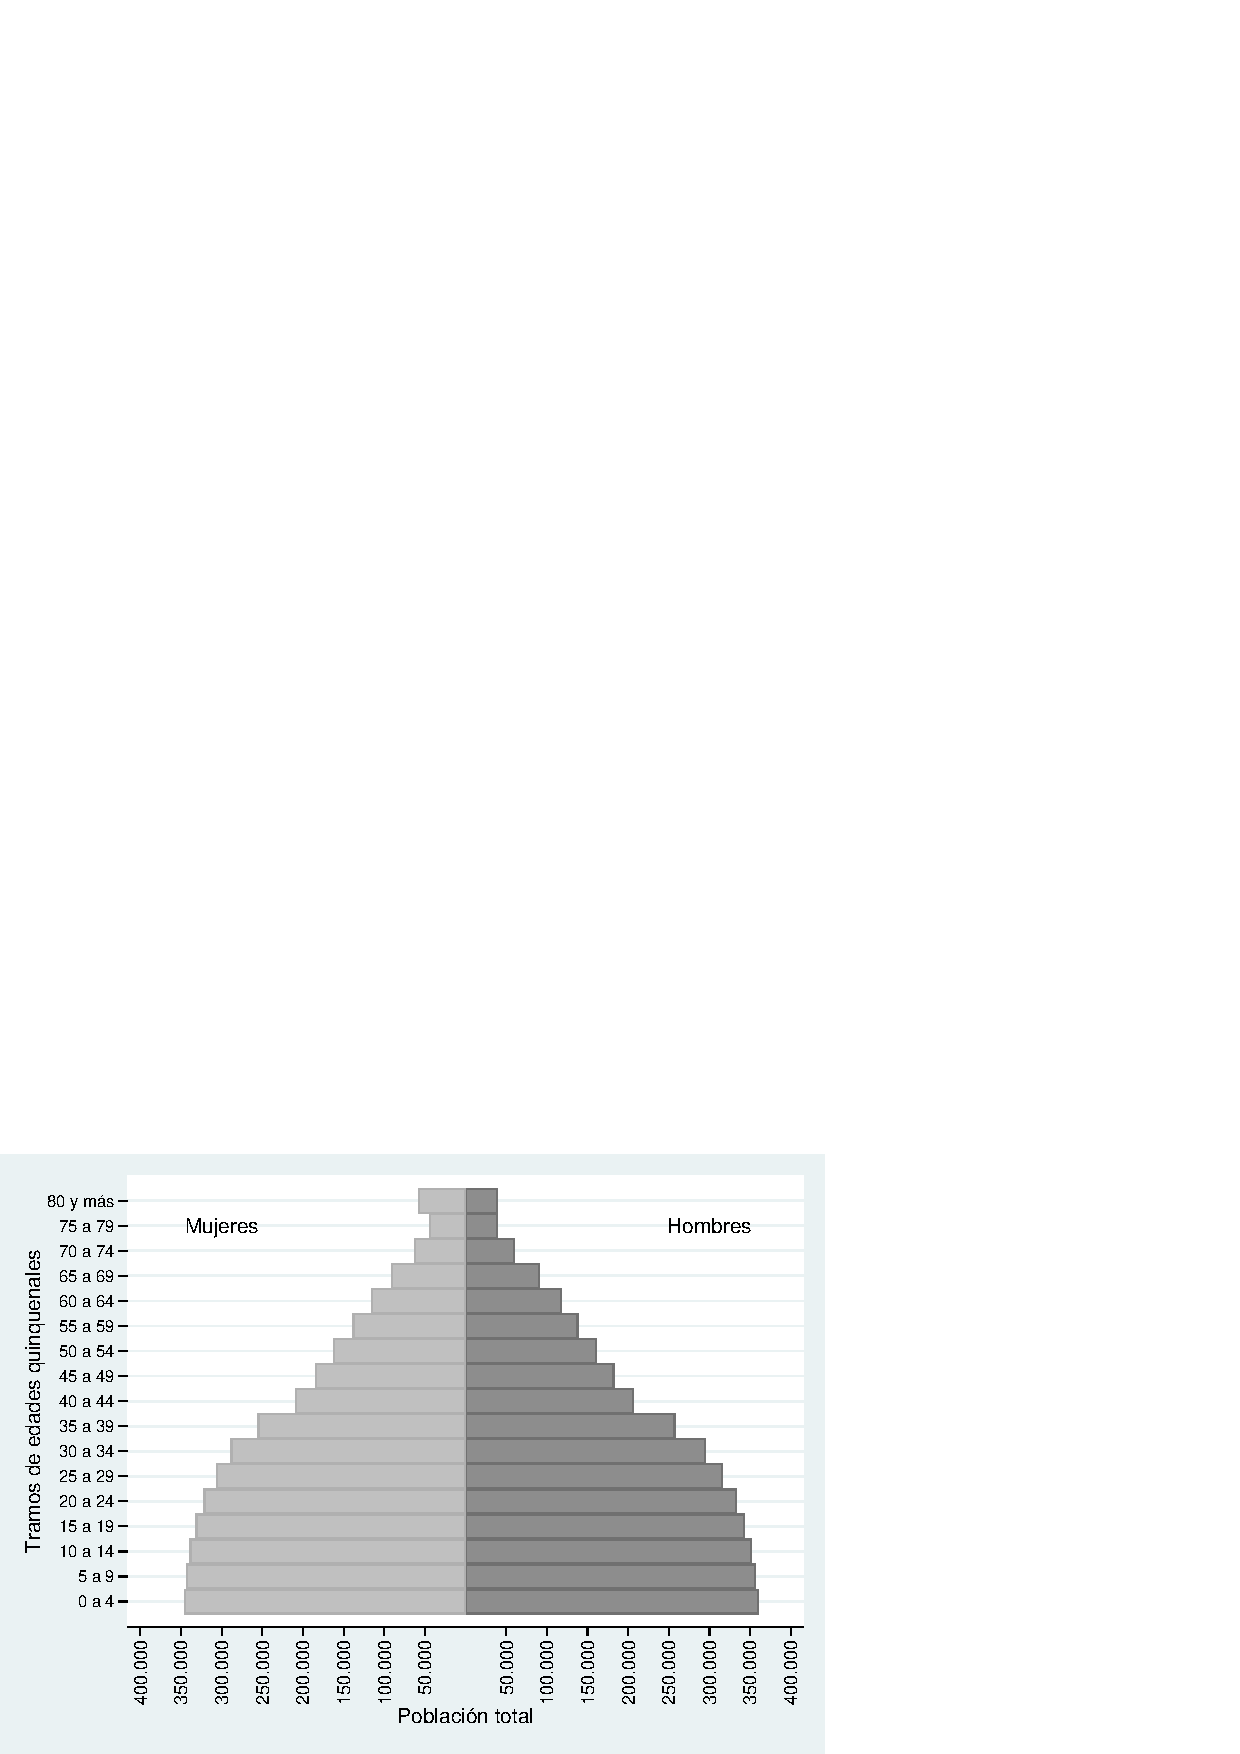
\includegraphics[scale=0.45]{indicadoresINE_pobtot_piramide.png}
                                    \item \footnotesize Fuente : Instituto Nacional de Estadística.
                    \end{center}
\end{figure}

\subsubsection{Esperanza de vida - Mortalidad}

La Esperanza de Vida es el promedio de años que se espera viva una
persona a partir de la edad que tiene, por lo que a la hora de analizar
un Sistema de Jubilaciones y Pensiones se necesita no sólo saber la
esperanza de vida al nacer sino también la esp eranza de vida de la
persona al momento de jubilarse, ya que esto representa cuantos años en
promedio se estarán pagando las jubilaciones.

En la evolución de la Esperanza de Vida al nacer por sexo, se puede
apreciar dos puntos relevantes: primero, en ambos sexos existe un
incremento en la esperanza de vida al nacer; y segundo, las mujeres
siempre tienen una expectativa de vida superior a l a de los hombres a
lo largo del periodo considerado.

Una expectativa de vida superior en las mujeres es una situación similar
a la que se presenta en los países de la región y en los países
desarrollados. El incremento de los años que se espera vivir en promedio
en Paraguay también es una evolución natur al debido a una mejora
continua en la calidad de vida mediante el acceso a los servicios
sanitarios (inmunizaciones, asistencia pediátrica) y servicios públicos
de suministro (agua, electricidad, alcantarillado sanitario).

La esperanza de vida al nacer de un hombre en Paraguay en el 2001 era de
67,6 años, mientras que la de una mujer era de 72,8 años. Para el año
2020 se estima que la esperanza de vida del hombre aumentó en 4,1 años
llegando a 71,7; en tanto que para la m ujer se incrementó en 4,9 años,
alcanzando la edad de 77,7. Esto evidencia una diferencia promedio en la
esperanza de vida de 5,6 años a favor de las mujeres a lo largo del
periodo analizado.

\begin{figure}[H]
\begin{center}
                    \caption{Esperanza de vida al nacer. Periodo 2001-2025}
                    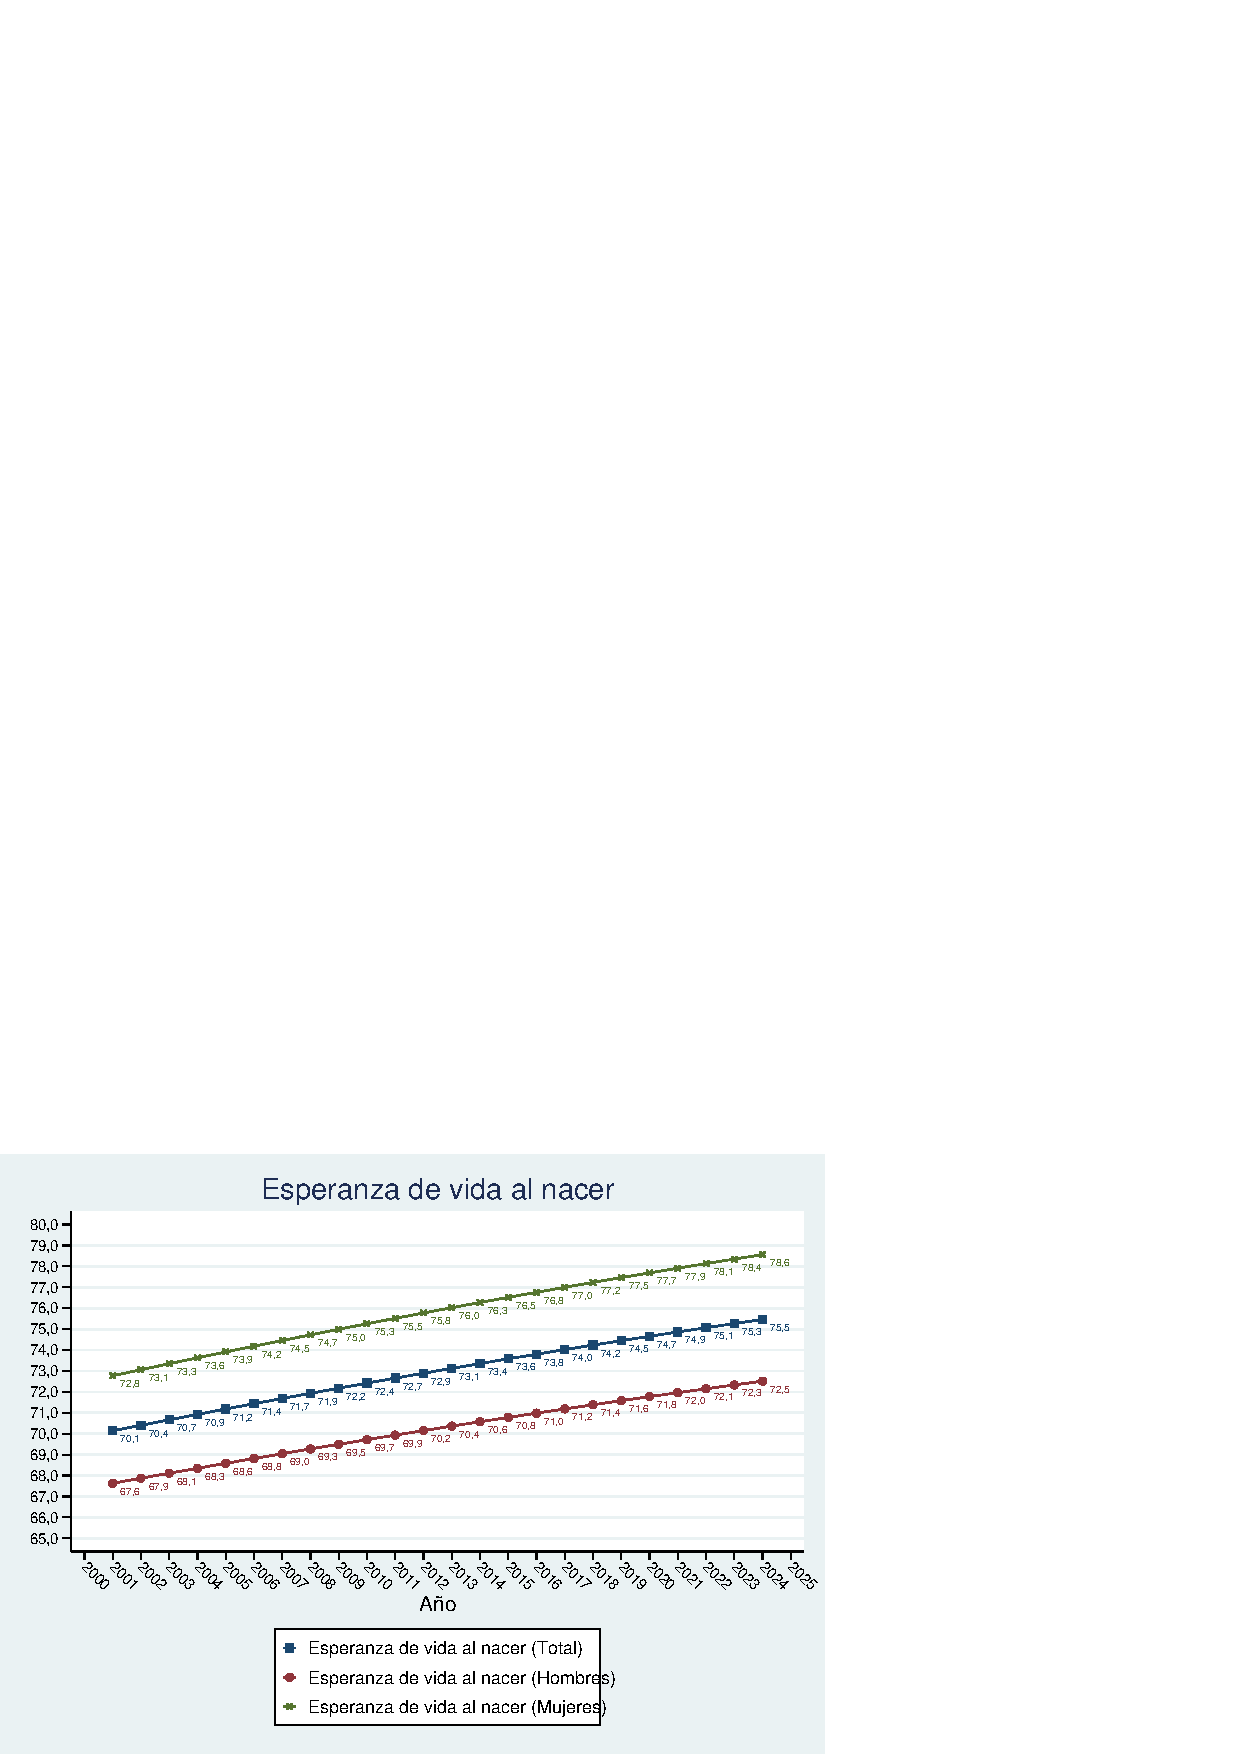
\includegraphics[scale=0.45]{INE_indic_ev0.png}
                                    \item \footnotesize Fuente : Instituto Nacional de Estadística.
                    \end{center}
\end{figure}

El número de muertes para el año 2001 en el Paraguay ascendía a 33.185.
Para el año 2025 se estima un incremento de 32,1\% en dicha cifra,
alcanzado un valor aproximado de 43.836 muertes por año.

\begin{figure}[H]
\begin{center}
                    \caption{Número de muertes por año. Periodo 2001-2025}
                    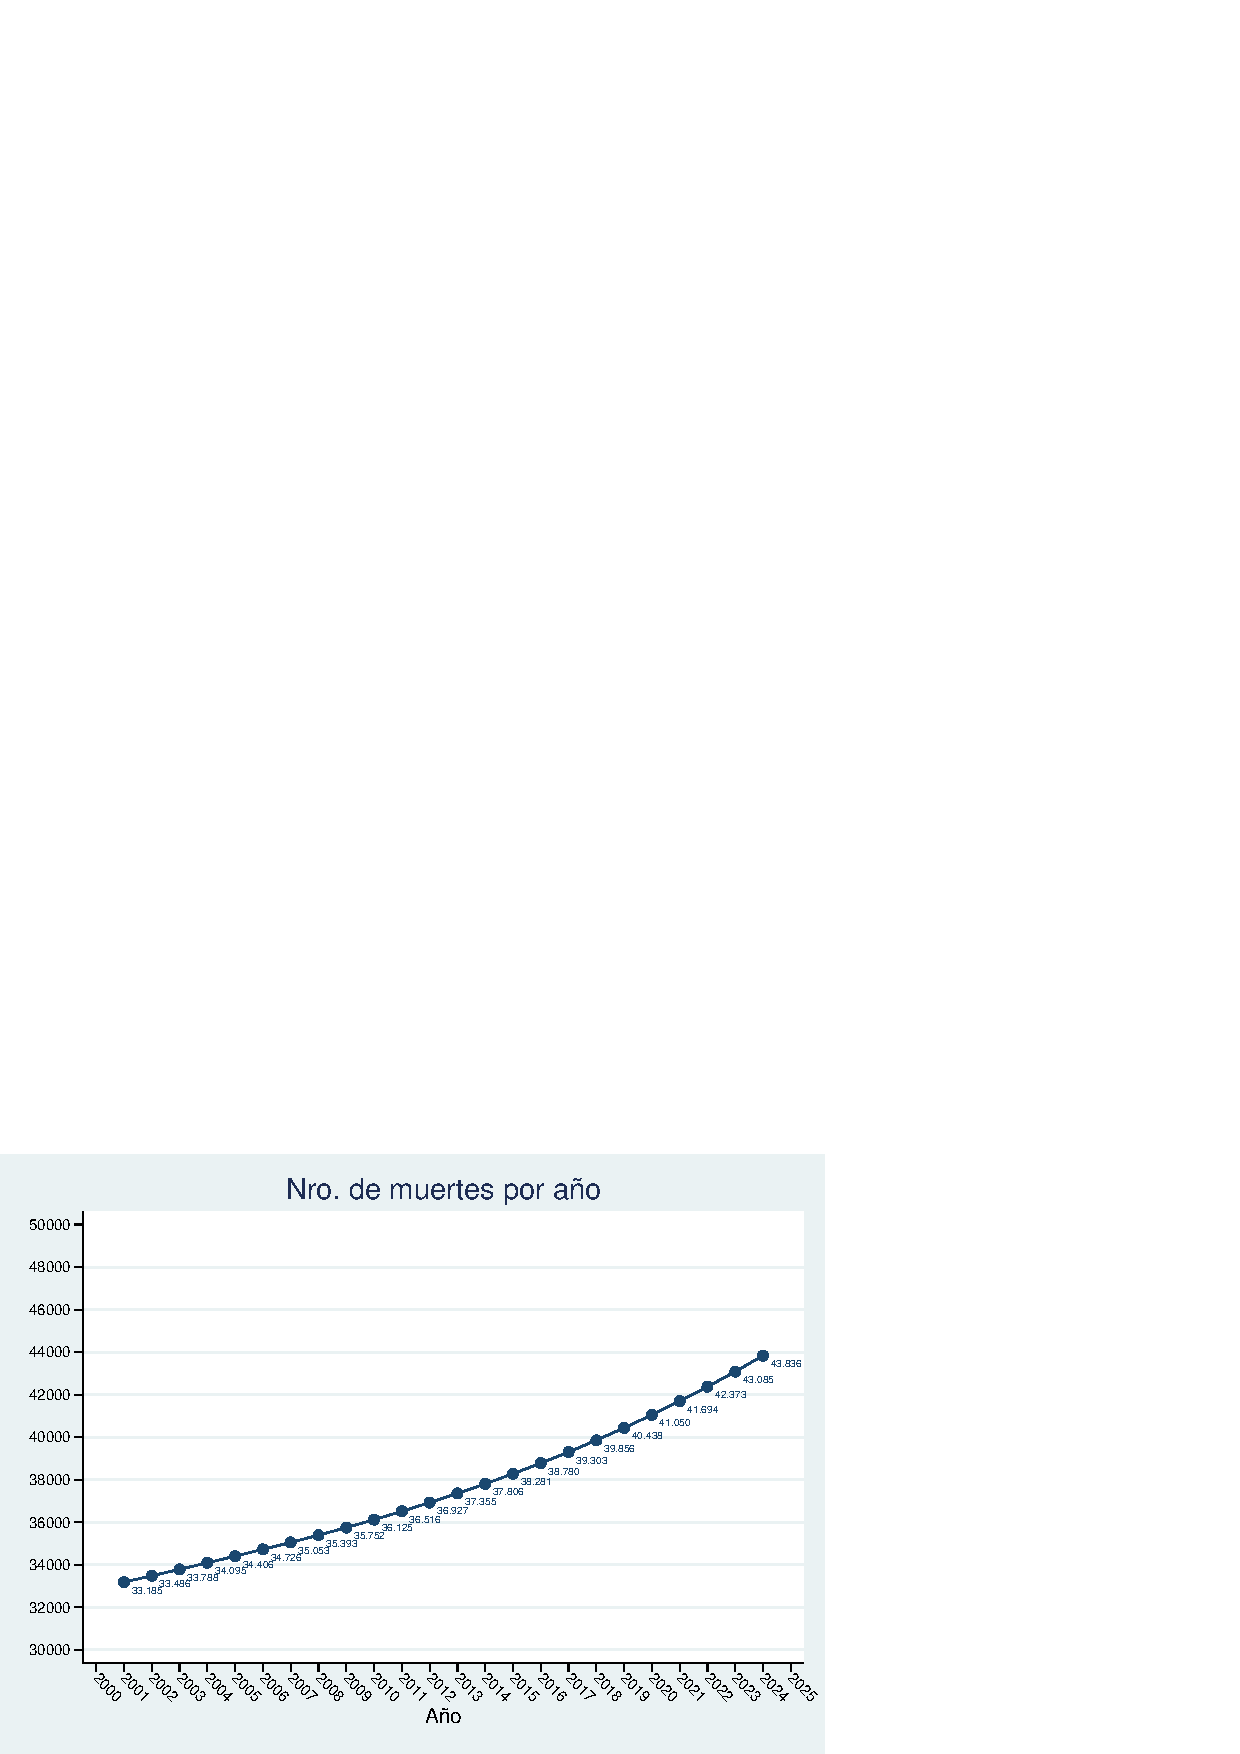
\includegraphics[scale=0.45]{INE_indic_nromuertesanual.png}
                                    \item \footnotesize Fuente : Instituto Nacional de Estadística.
                    \end{center}
\end{figure}

Si bien existe una mejora en la probabilidad de supervivencia para todas
las edades, la principal mejora se da en las edades más jóvenes, lo que
da indicio de que la pirámide poblacional irá ensanchándose, es decir,
la forma de la distribución irá cambi ando lentamente de una forma
piramidal hacia una más rectangular.

En cuanto a la evolución de la esperanza de vida a los 60 años para
hombres y mujeres en el Paraguay, en el año 2000 se pagaba jubilaciones
a una persona de 60 años, en promedio durante 19,4 años si era hombre y
21,9 si era mujer, mientras que para el a ño 2020 se adiciona 1,4 años
para los hombres y 2,3 años a las mujeres para el mismo fin.

\begin{figure}[H]
\begin{center}
                    \caption{Esperanza de vida a los 60 años por sexo, según periodo}
                    \includegraphics[scale=0.45]{INE_indic_ex_periodo_60.png}
                    \item \footnotesize Fuente : Instituto Nacional de Estadística.
                    \end{center}
\end{figure}

\subsubsection{Fecundidad}

De manera sencilla, se puede definir la Tasa Global de Fecundidad
(TGF)\footnote{ De manera formal, CELADE define la Tasa Global de Fecundidad como "el número de hijos que en promedio tendría una mujer de una cohorte hipotética de mujeres que durante su
 vida fértil tuvieran sus hijos de acuerdo a las tasas de fecundidad por edad del período en estudio y no estuvieran expuestas a riesgos de mortalidad desde el nacimiento hasta el término del período fértil" (CELADE, 2017).}
como ``el número de hijos en promedio que tiene una mujer durante toda
su vida
fértil\footnote{ Se considera que la mujer se encuentra en edad reproductiva (edad fértil) entre los 15 y 49 años.}''.

Si bien a la hora de proyectar la población se utilizan tasas de
fecundidad por edad simple, la TGF es un indicador de la tendencia en la
fecundidad y finalmente cómo se espera que evolucione la población.

Al presentar la evolución de la TGF en Paraguay, se puede apreciar una
clara tendencia decreciente, pasando de 3,4 hijos por mujer en el año
2001 a 2,4 hijos por mujer en el año 2020.

El aumento de la esperanza de vida va acompañado de una disminución de
la tasa de fecundidad, factor que también incide en el ensanchamiento de
la pirámide de población.

Según datos del INE, para el año 2025 se estima un total de 145.228
nacimientos en el país.

\begin{figure}[H]
\begin{center}
                    \caption{Número de nacimientos por año. Periodo 2001-2025}
                    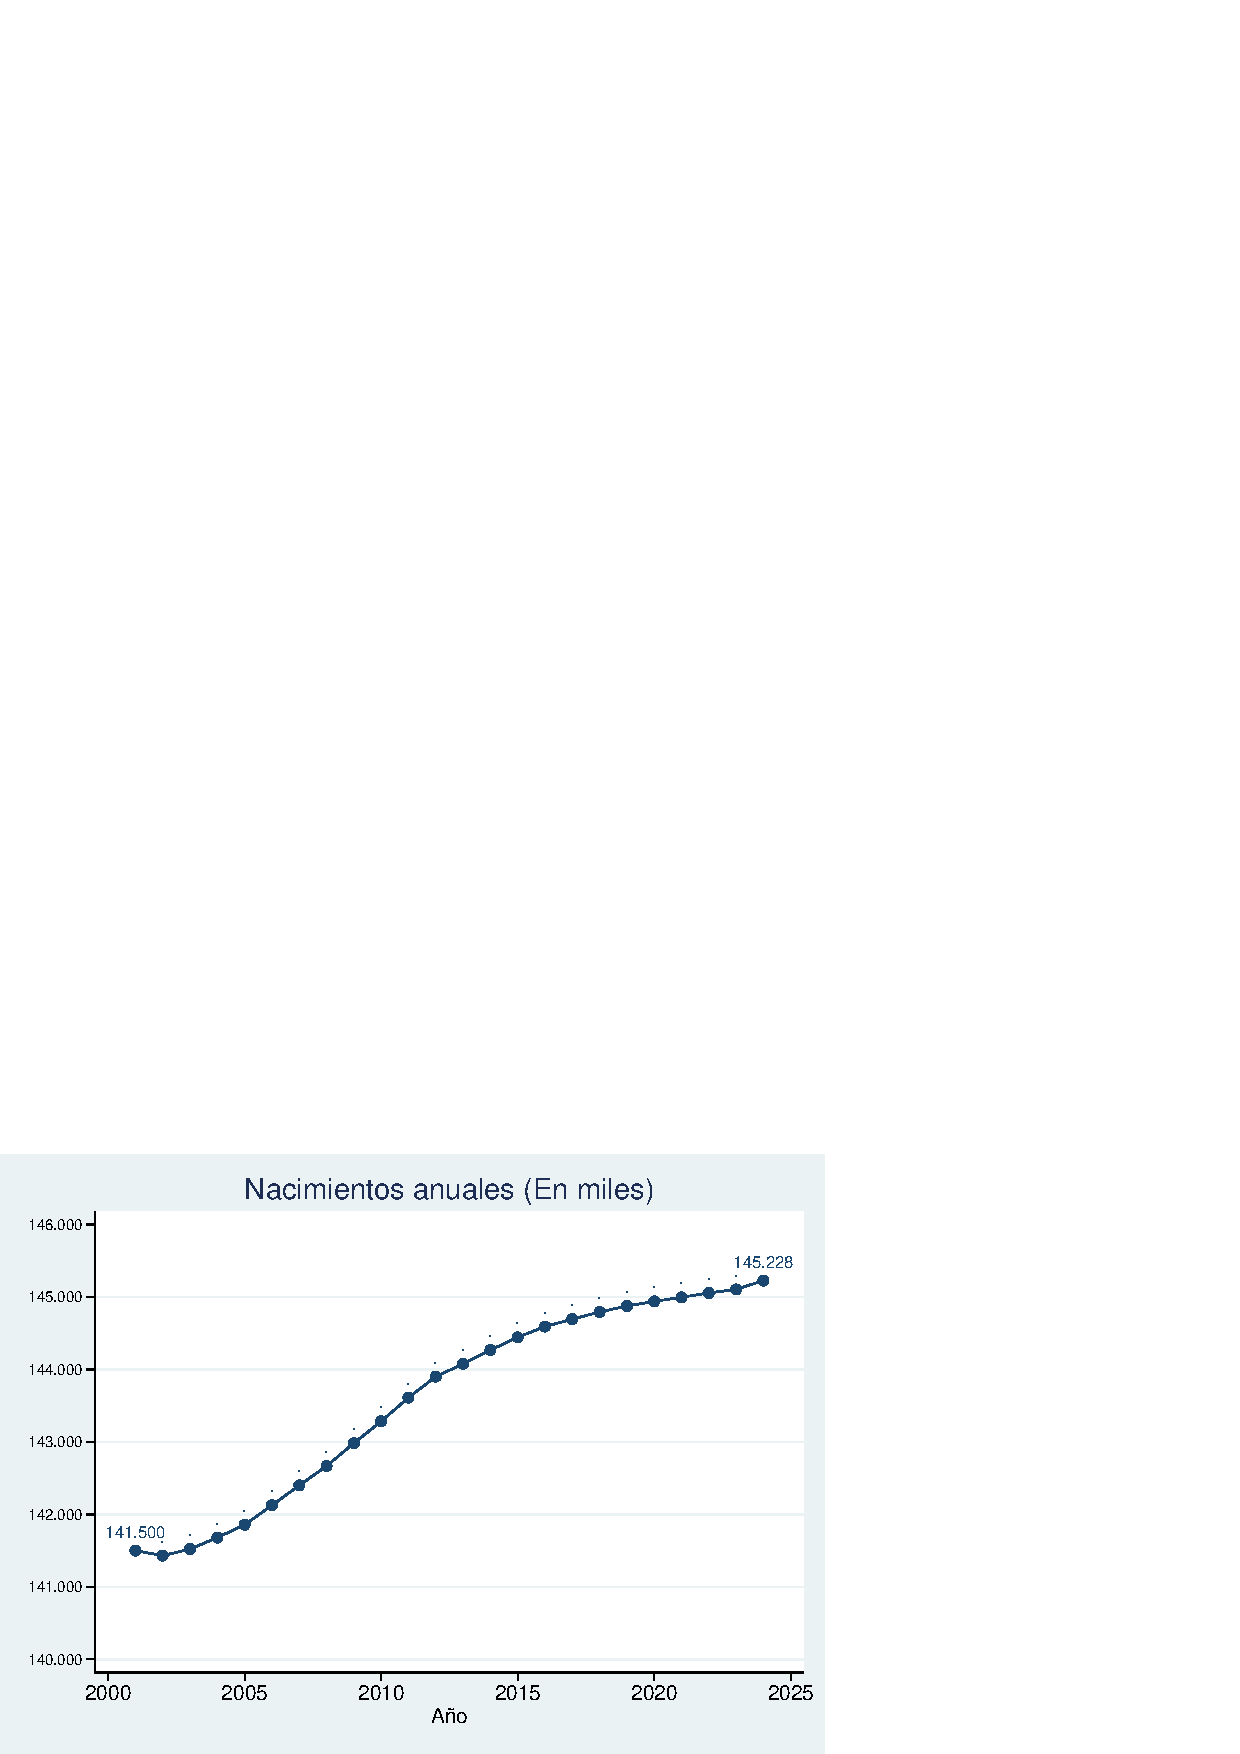
\includegraphics[scale=0.45]{INEnronacanual.png}
                                    \item \footnotesize Fuente : Instituto Nacional de Estadísticas.

                    \end{center}
\end{figure}

\begin{figure}[H]
\begin{center}
                    \caption{Tasa global de fecundidad. Periodo 2001-2025}
                    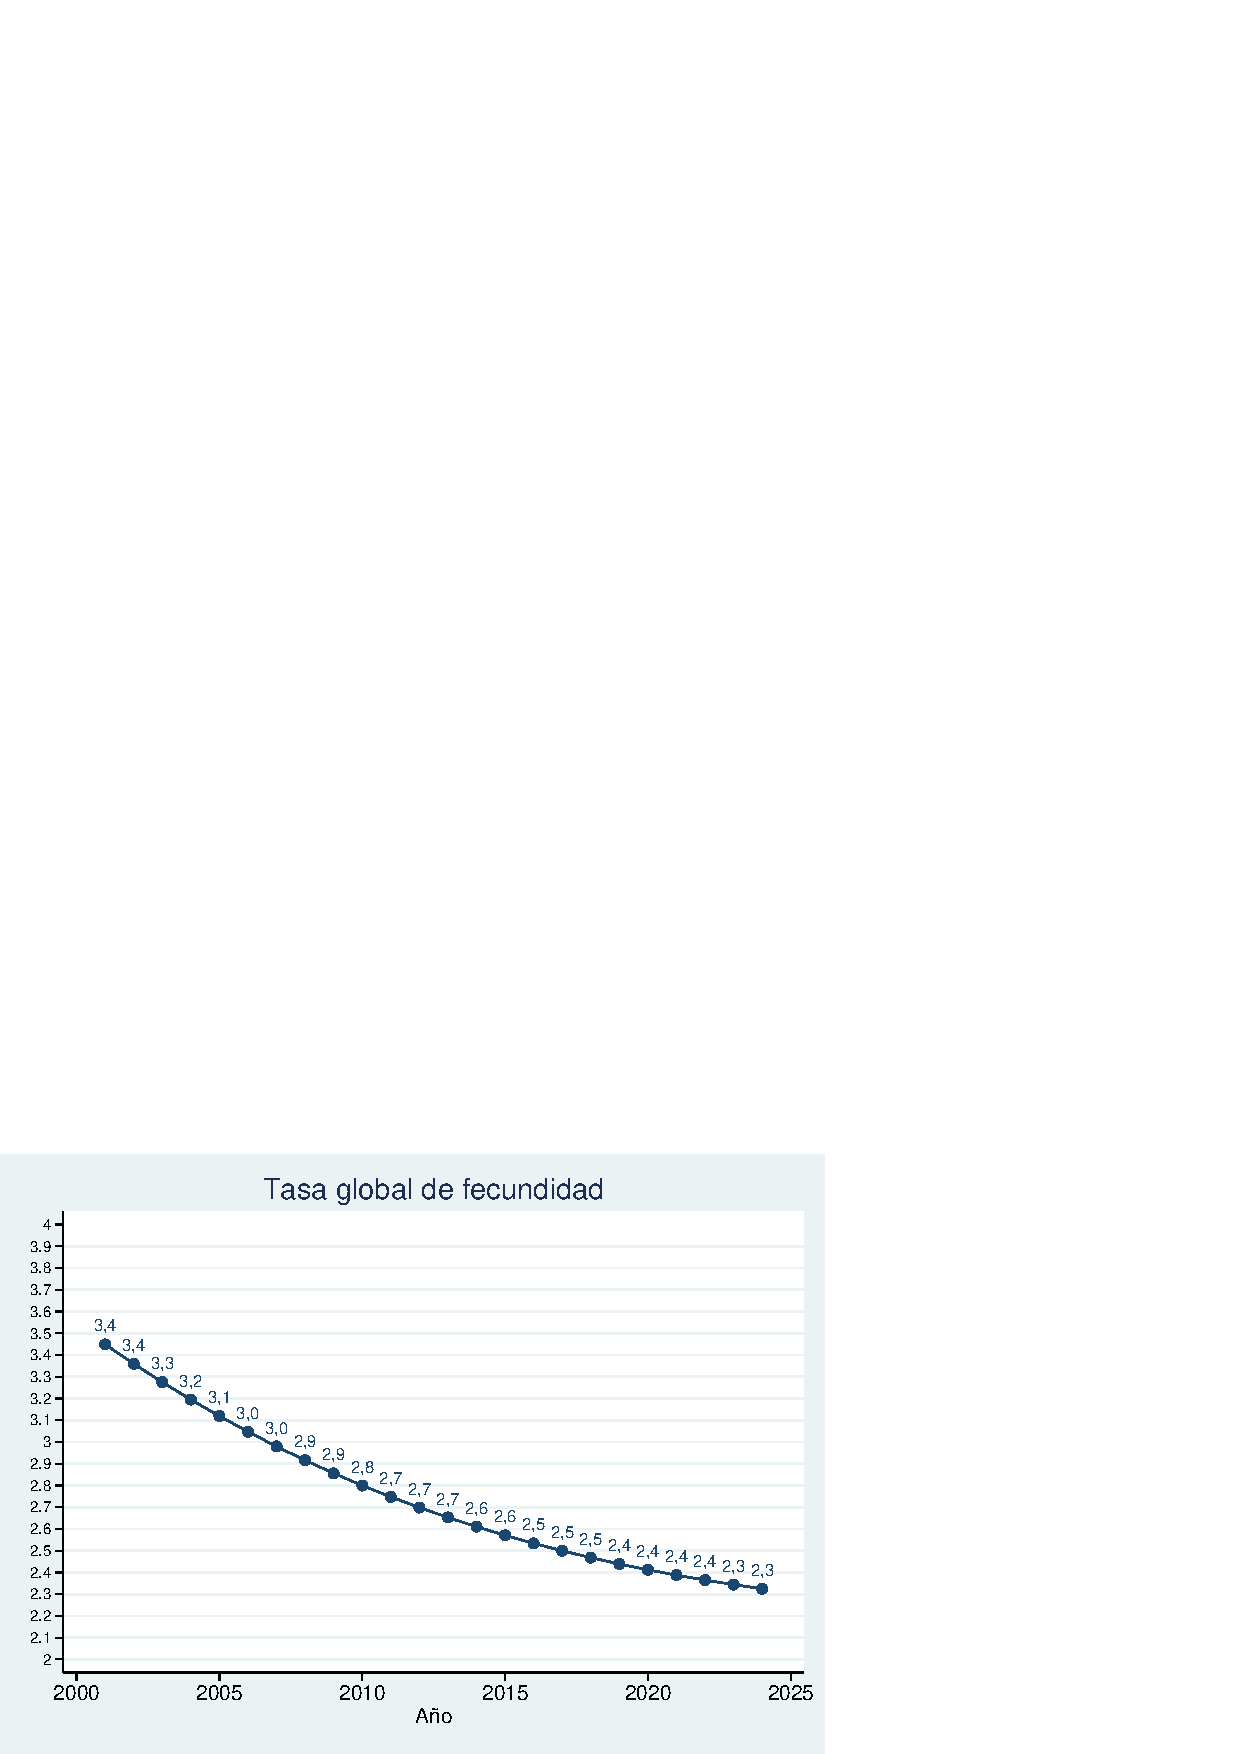
\includegraphics[scale=0.45]{INEtasaglobalfecun.png}
                                    \item \footnotesize Fuente : Instituto Nacional de Estadística.
\end{center}
\end{figure}

\subsubsection{Índice de Masculinidad. Periodo 2000-2025}

El índice de masculinidad, también llamado ``razón de sexo'' es un
índice demográfico que expresa la razón de hombres frente a mujeres en
un determinado territorio, enunciada en tanto por ciento. Se calcula
dividiendo la cantidad total de hombres por la cantidad total de
mujeres.

En el año 2000 había 102,3 hombres por cada 100 mujeres en el Paraguay
\footnote{STP/DGEEC. Paraguay. Proyección de la Población Nacional, Áreas Urbana y Rural por Sexo y Edad, 2000-2025. Revisión 2015.},
estimándose a 101,1 hombres por cada 100 mujeres para el año 2025.

\begin{figure}[H]
\begin{center}
                    \caption{Índice de Masculinidad}
                    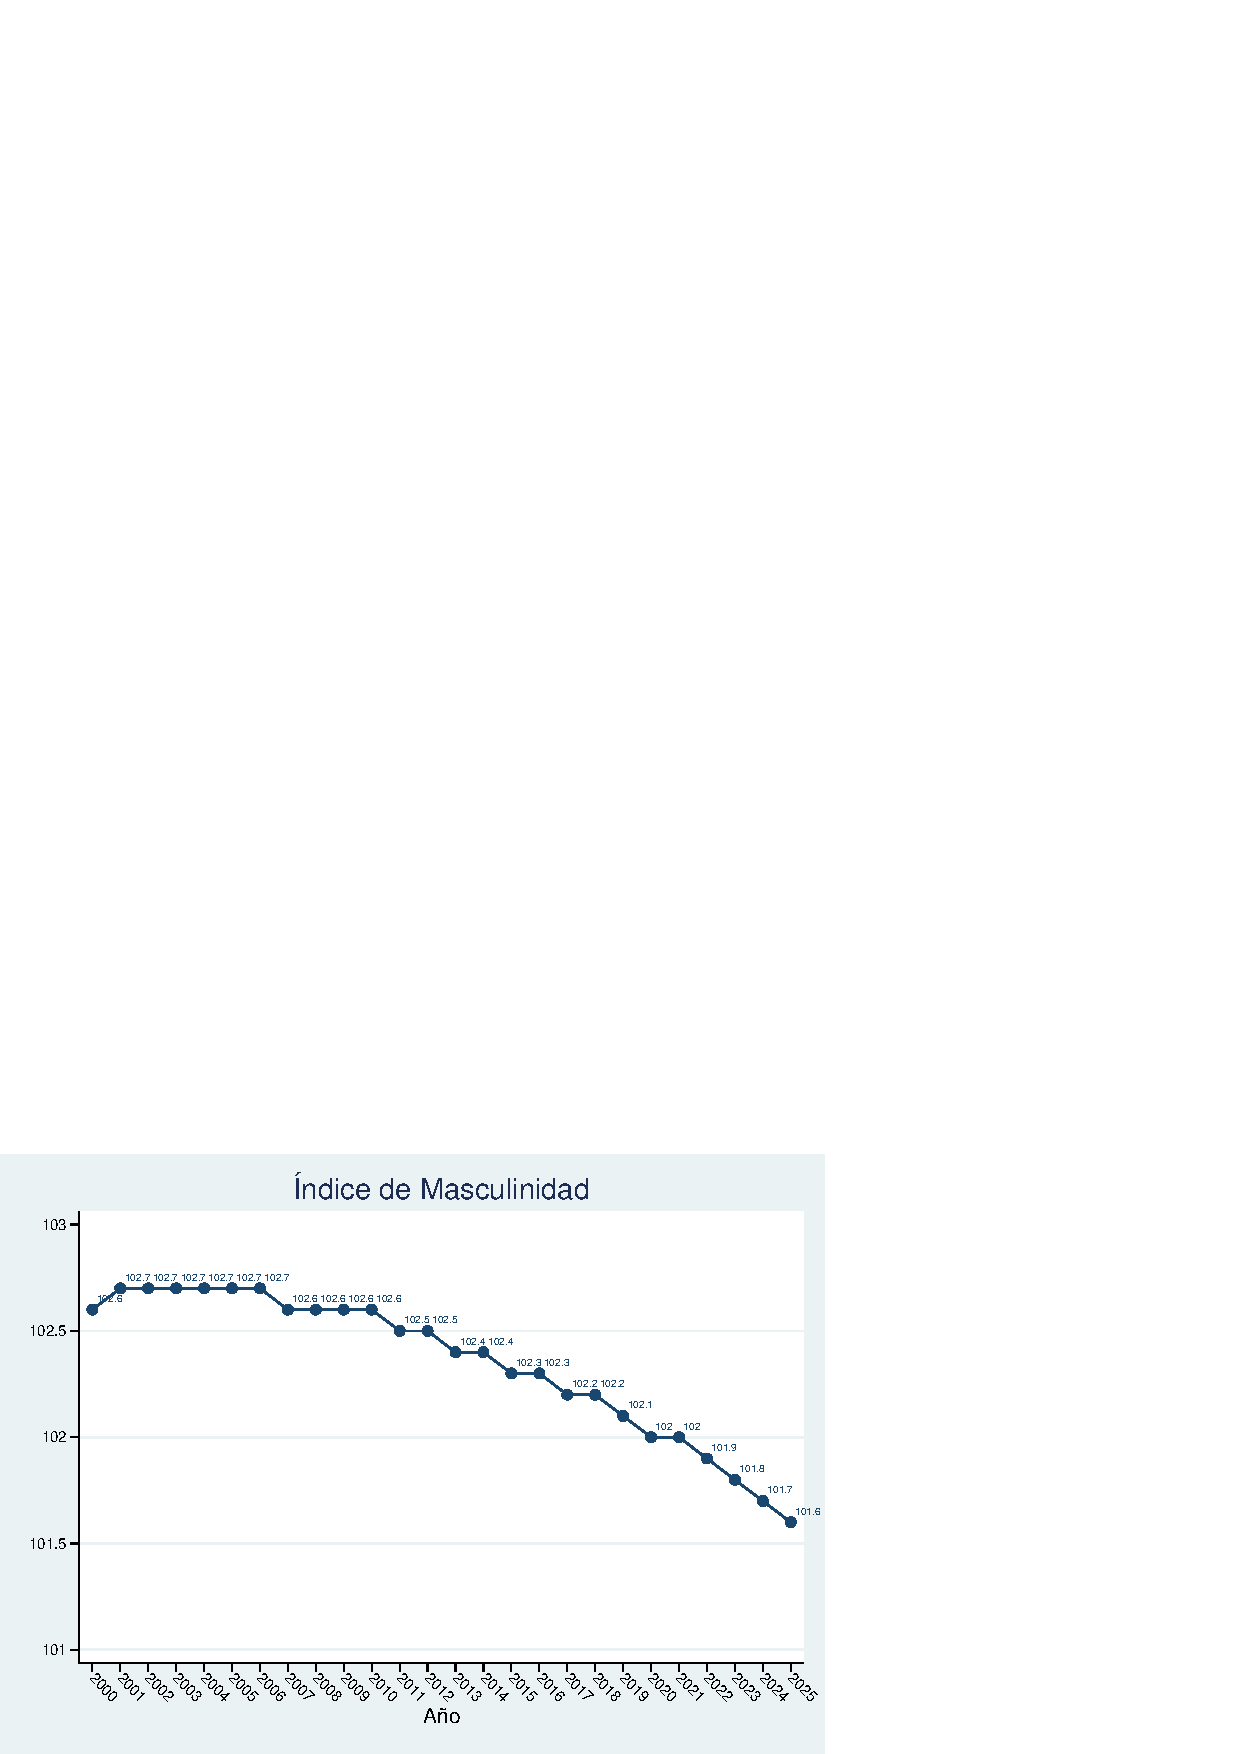
\includegraphics[scale=0.45]{INE_indic_masc.png}
                                    \item \footnotesize Fuente : Instituto Nacional de Estadística.
                    \end{center}
\end{figure}

Esta tasa también es calculada al momento del nacimiento, denominada
Tasa Específica de Masculinidad y es obtenida dividiendo la cantidad de
recién nacidos del sexo masculino con la cantidad de recién nacidos del
sexo femenino.

Al visualizar las tasas global y específica de masculinidad, el interés
recae en la segunda por ser la utilizada como insumo de las proyecciones
actuariales. De los datos históricos y proyectados, se aprecia que la
Tasa Específica de Masculinidad se man tuvo constante en todo el
periodo, promediando un valor muy próximo a 104 hombres por cada 100
mujeres. **** esta evolución no está en el overleaf***

\subsubsection{Migraciones}

El INE ha calculado el saldo neto migratorio recurriendo a varias
fuentes, entre las que se pueden citar los registros oficiales de
entradas y salidas, los censos de población y viviendas nacionales y de
otros países. Como en toda proyección, el saldo m igratorio o migración
neta, es el componente que en principio más influiría en la
incertidumbre respecto al tamaño y estructura futura de la población.

Sin embargo, a menos que se trate de movimientos sustanciales y
persistentes en el tiempo, su efecto no es significativo.

Al observar los datos históricos y la estimación de la migración
internacional neta para el periodo 2001-2025, el Paraguay ha tenido un
saldo negativo en las migraciones netas que fue aumentando hasta el año
2009 donde se observa un cambio en la tendenc ia. A partir del año 2010
ese saldo negativo ha ido disminuyendo y se estima un valor cercano a 0
(cero) para el año 2025.

\begin{figure}[H]
\begin{center}
                    \caption{Migración anual (en miles). Periodo 2001-2025}
                    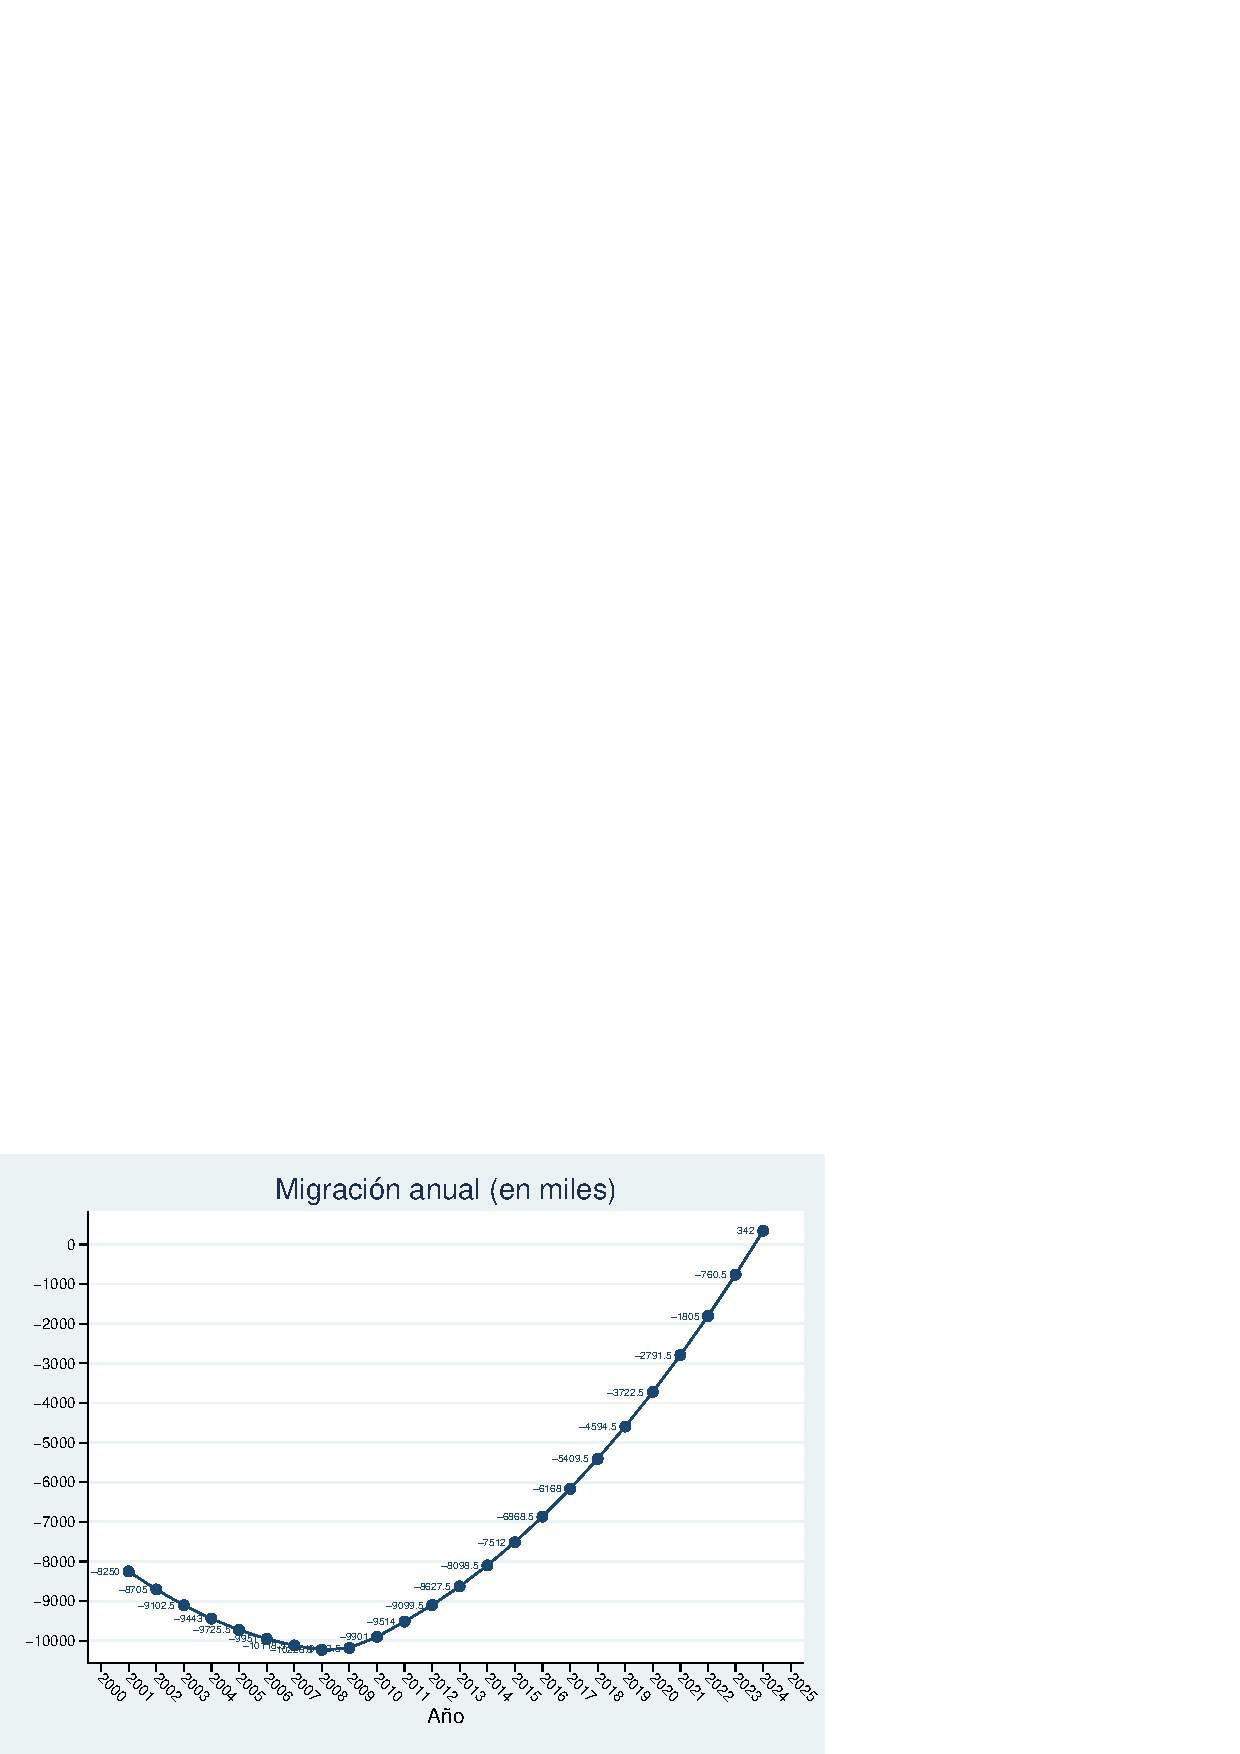
\includegraphics[scale=0.45]{INE_indic_miganaul.png}
                                    \item \footnotesize Fuente : Instituto Nacional de Estadística.
                    \end{center}
\end{figure}

\begin{figure}[H]
\begin{center}
                    \caption{Tasa de migración (por mil). Periodo 2001-2025}
                    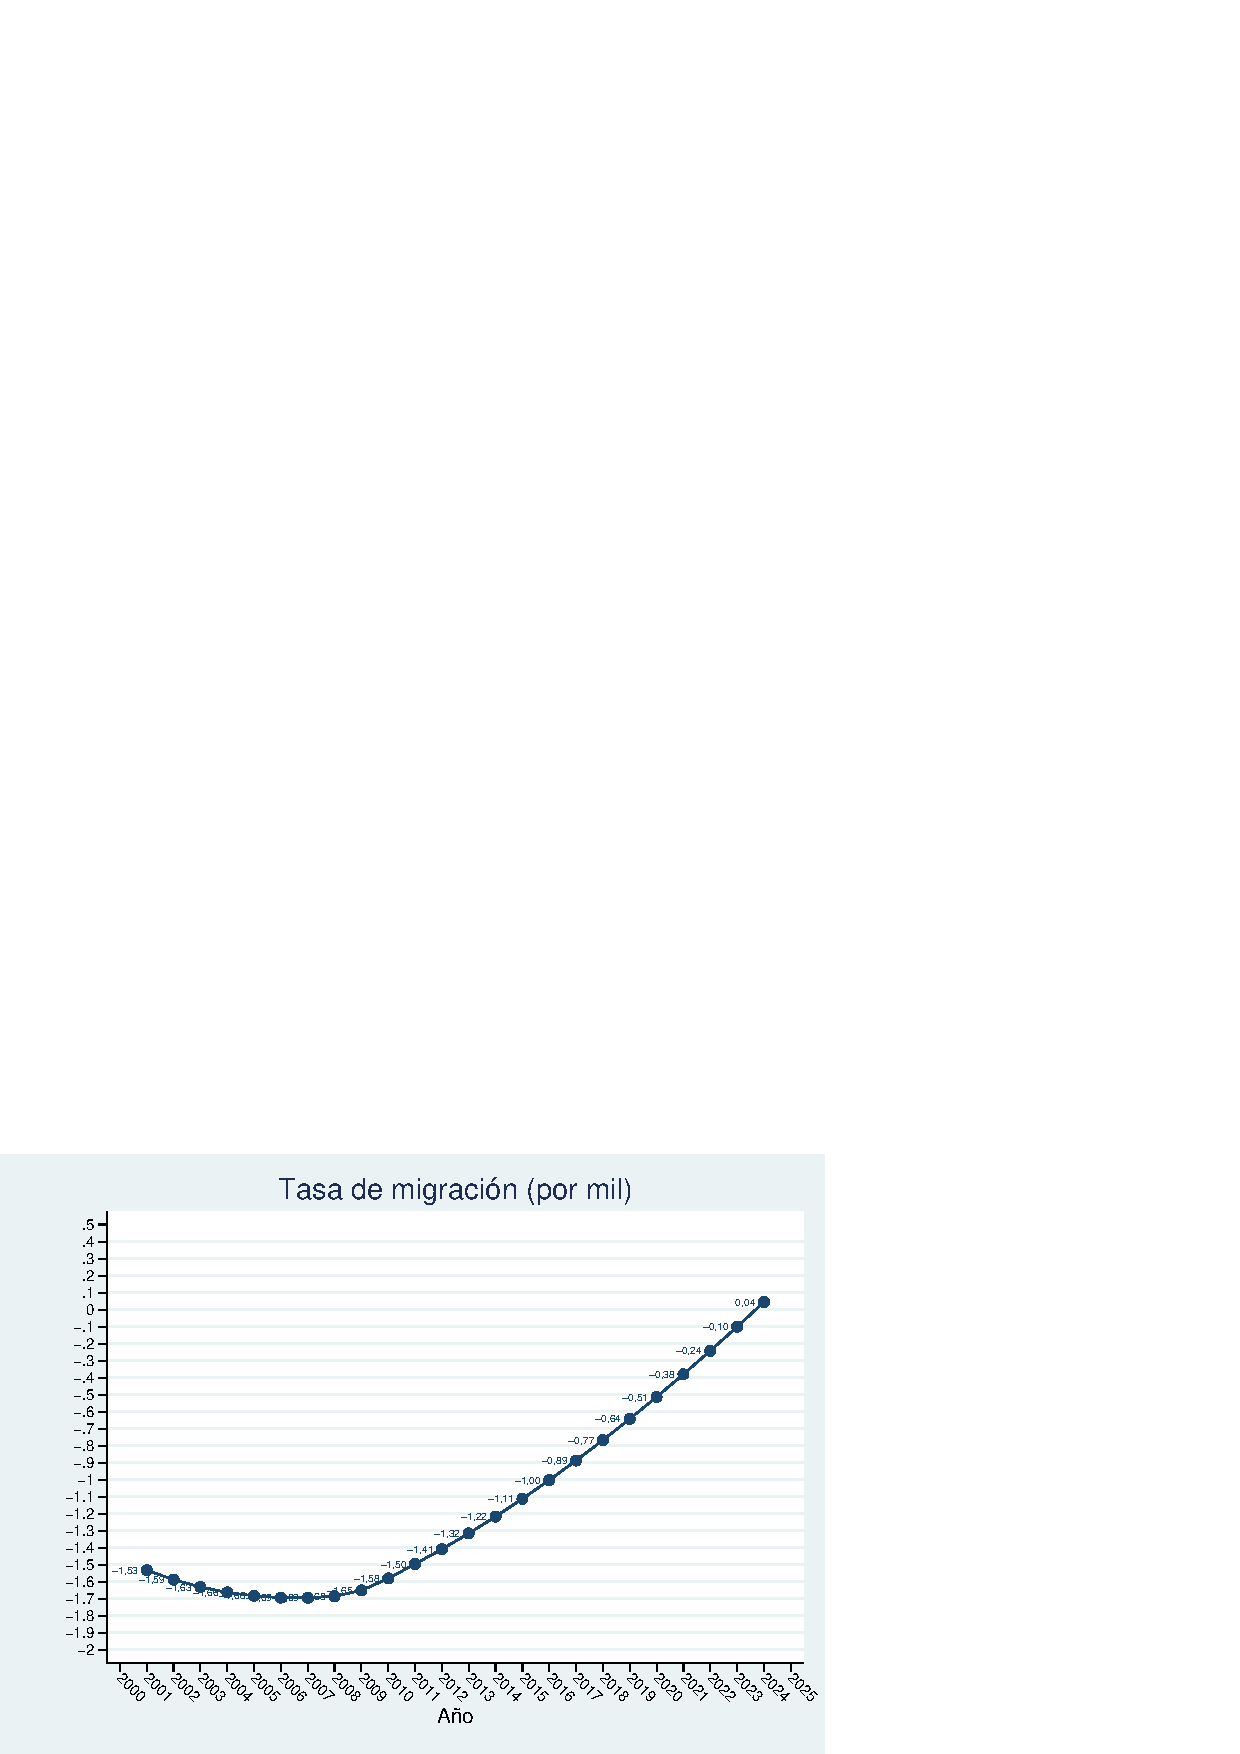
\includegraphics[scale=0.45]{INE_indic_tasamig.png}
                                    \item \footnotesize Fuente : Instituto Nacional de Estadística.
                    \end{center}
\end{figure}

\newpage
\newpage

\subsection{Contexto laboral}\subsubsection{Actividad y Ocupación}

En el Sistema de Jubilaciones y Pensiones administrado por el IPS, la
financiación se encuentra basada en los aportes obrero-patronales de los
asalariados, por lo que conocer el universo de potenciales afiliados es
de vital importancia.

Las estadísticas relacionadas al mercado de trabajo se obtienen de la
EPH. De acuerdo con estos datos, la población paraguaya total en el año
2020 es de 7.167.516 personas, de los cuales 5.094.469 tienen 15 o más
años de edad, que para los fines de este informe será considerada como
la población en edad de trabajar (PET), ésta representa un 71,1\% de la
población total. Una subpoblación de interés es la Población
Económicamente Activa (PEA) también llamada Fuerza de
Trabajo\footnote{Fuerza de trabajo, también conocida como Población Económicamente Activa (PEA) de acuerdo a la 19ª Conferencia Internacional de Estadístic
as del Trabajo - CIET.}, la cual está conformada por las personas
ocupadas y desocupadas. La Fuerza de Trabajo en Paraguay está compuesta
por un total de 3.678.114 de personas, que representan el 72,2\% de la
PET \footnote{Este resultado difiere de las 
publicaciones oficiales del INE por la definición especial considerada para la población en edad de trabajar.}.

La tasa de desocupación o desempleo abierto afectó en el año 2020 al
7,0\% de la PEA, lo que implica que alrededor de 256.678 personas
estaban sin trabajo y buscaron activamente empleo en el periodo de
referencia de la encuesta (últimos 7 días).

La estructura de la población con respecto a estos indicadores del
mercado laboral de las personas con 15 y más años de edad, para el
periodo 2013-2020, se presenta en la Tabla 2.

\begin{table}[H]
\begin{center}
\footnotesize
\caption{\bf{Estructura de la población. Periodo 2013-2020}}
\begin{tabular}{l|rrrrrr}
\begin{tabular}{llllllll}
\cline{1-8}
\multicolumn{1}{c}{} &
  \multicolumn{1}{|r}{PT} &
  \multicolumn{1}{r}{PET} &
  \multicolumn{1}{r}{PEA} &
  \multicolumn{1}{r}{PEI} &
  \multicolumn{1}{r}{PO} &
  \multicolumn{1}{r}{PD} &
  \multicolumn{1}{r}{NR} \\
\cline{1-8}
\multicolumn{1}{l}{Año} &
  \multicolumn{1}{|r}{} &
  \multicolumn{1}{r}{} &
  \multicolumn{1}{r}{} &
  \multicolumn{1}{r}{} &
  \multicolumn{1}{r}{} &
  \multicolumn{1}{r}{} &
  \multicolumn{1}{r}{} \\
\multicolumn{1}{l}{\hspace{1em}2013} &
  \multicolumn{1}{|r}{6.485.377} &
  \multicolumn{1}{r}{4.422.659} &
  \multicolumn{1}{r}{3.156.825} &
  \multicolumn{1}{r}{1.265.630} &
  \multicolumn{1}{r}{2.997.615} &
  \multicolumn{1}{r}{159.210} &
  \multicolumn{1}{r}{204} \\
\multicolumn{1}{l}{\hspace{1em}2014} &
  \multicolumn{1}{|r}{6.581.971} &
  \multicolumn{1}{r}{4.535.155} &
  \multicolumn{1}{r}{3.166.411} &
  \multicolumn{1}{r}{1.368.744} &
  \multicolumn{1}{r}{2.976.862} &
  \multicolumn{1}{r}{189.549} &
  \multicolumn{1}{r}{0} \\
\multicolumn{1}{l}{\hspace{1em}2015} &
  \multicolumn{1}{|r}{6.678.731} &
  \multicolumn{1}{r}{4.657.248} &
  \multicolumn{1}{r}{3.233.111} &
  \multicolumn{1}{r}{1.424.137} &
  \multicolumn{1}{r}{3.061.380} &
  \multicolumn{1}{r}{171.731} &
  \multicolumn{1}{r}{0} \\
\multicolumn{1}{l}{\hspace{1em}2016} &
  \multicolumn{1}{|r}{6.775.786} &
  \multicolumn{1}{r}{4.710.766} &
  \multicolumn{1}{r}{3.322.812} &
  \multicolumn{1}{r}{1.387.177} &
  \multicolumn{1}{r}{3.122.747} &
  \multicolumn{1}{r}{200.065} &
  \multicolumn{1}{r}{777} \\
\multicolumn{1}{l}{\hspace{1em}2017} &
  \multicolumn{1}{|r}{6.873.496} &
  \multicolumn{1}{r}{4.821.570} &
  \multicolumn{1}{r}{3.406.276} &
  \multicolumn{1}{r}{1.415.294} &
  \multicolumn{1}{r}{3.228.636} &
  \multicolumn{1}{r}{177.640} &
  \multicolumn{1}{r}{0} \\
\multicolumn{1}{l}{\hspace{1em}2018} &
  \multicolumn{1}{|r}{6.971.229} &
  \multicolumn{1}{r}{4.897.047} &
  \multicolumn{1}{r}{3.517.575} &
  \multicolumn{1}{r}{1.379.472} &
  \multicolumn{1}{r}{3.317.775} &
  \multicolumn{1}{r}{199.800} &
  \multicolumn{1}{r}{0} \\
\multicolumn{1}{l}{\hspace{1em}2019} &
  \multicolumn{1}{|r}{7.069.327} &
  \multicolumn{1}{r}{4.988.971} &
  \multicolumn{1}{r}{3.626.368} &
  \multicolumn{1}{r}{1.362.603} &
  \multicolumn{1}{r}{3.422.331} &
  \multicolumn{1}{r}{204.037} &
  \multicolumn{1}{r}{0} \\
\multicolumn{1}{l}{\hspace{1em}2020} &
  \multicolumn{1}{|r}{7.167.516} &
  \multicolumn{1}{r}{5.094.469} &
  \multicolumn{1}{r}{3.678.114} &
  \multicolumn{1}{r}{1.416.355} &
  \multicolumn{1}{r}{3.421.436} &
  \multicolumn{1}{r}{256.678} &
  \multicolumn{1}{r}{0} \\
\cline{1-8}
\end{tabular}

\end{tabular}
                    \item \footnotesize Fuente : Encuesta Permanente de Hogares. 
                    \item \footnotesize Nota : PT (Población Total), PET (Población en Edad de Trabajar) PEA (Población Económicamente Activa), PEI (Población Económicamente Inactiva), PO (Población Ocupada), PD (Población Desocupada) NR (No Responde). 
\end{center}
\end{table}

\begin{center}
\end{center}\begin{figure}[!ht]
                    \caption{Estructura del mercado de trabajo. Año 2020}
  \centering
  \hspace*{-80pt}
  \begin{tikzpicture}[node distance = 1cm, auto]
  
          % Place nodes
    \node [block] (p) { \textbf{Población Total} 7.167.516 (100\%)};
    \node [block,  below left=1cm and -0.3cm of p](pet) {\textbf{Población en Edad de Trabajar  (mayor a 14 años)} 5.094.469 (71.07\%)};
    \node [block,  below right=1cm and -0.3cm of p](pm15) {\textbf{Población menor a 15 años} 2.073.047. (28.92\%)};
    \node [block,  below left=1cm and -0.3cm of pet](pea) {\textbf{Población Económicamente Activa (PEA)} 3.678.114 (72.84\%)};
    \node [block,  below right=1cm and -0.3cm of pet](pei) {\textbf{{Población Económicamente} Inactiva} 1.416.355. (28.04\%)};
         \node [block,  below left=1cm and -0.3cm of pea](o) {\textbf{Ocupados} 3.421.436 (93.02\%)};
    \node [block,  below right=1cm and -0.3cm of pea](d) {\textbf{Desocupados} 256.678 (6.97\%)}; 
    % edges
         \path [line] (p) -- (pet);
         \path [line] (p) -- (pm15);
         \path [line] (pet) -- (pea);
         \path [line] (pet) -- (pei);
         \path [line] (pea) -- (o);
         \path [line] (pea) -- (d);
  \end{tikzpicture}
\end{figure}

La Tasa de Actividad se define como el cociente entre la Población
Económicamente Activa y la Población en Edad de Trabajar de 15 y más
años de edad, en tanto que la Tasa de Ocupación se calcula como el
cociente entre la Población Ocupada y la Población Económicamente
Activa.

Al observar la evolución de dichas tasas para el periodo 2013-2020, no
se presentan variaciones significativas entre los años 2013 y 2019. En
tanto que, para el año 2020 se aprecia una leve disminución de la tasa
de ocupación en 1,35 puntos porcentuales , pasando de 94,37\% en el año
2019 a 93,02\% para el año 2020.

\begin{figure}[H]
\begin{center}
                    \caption{Tasas de Actividad y Ocupación. Periodo 2013-2020}
                    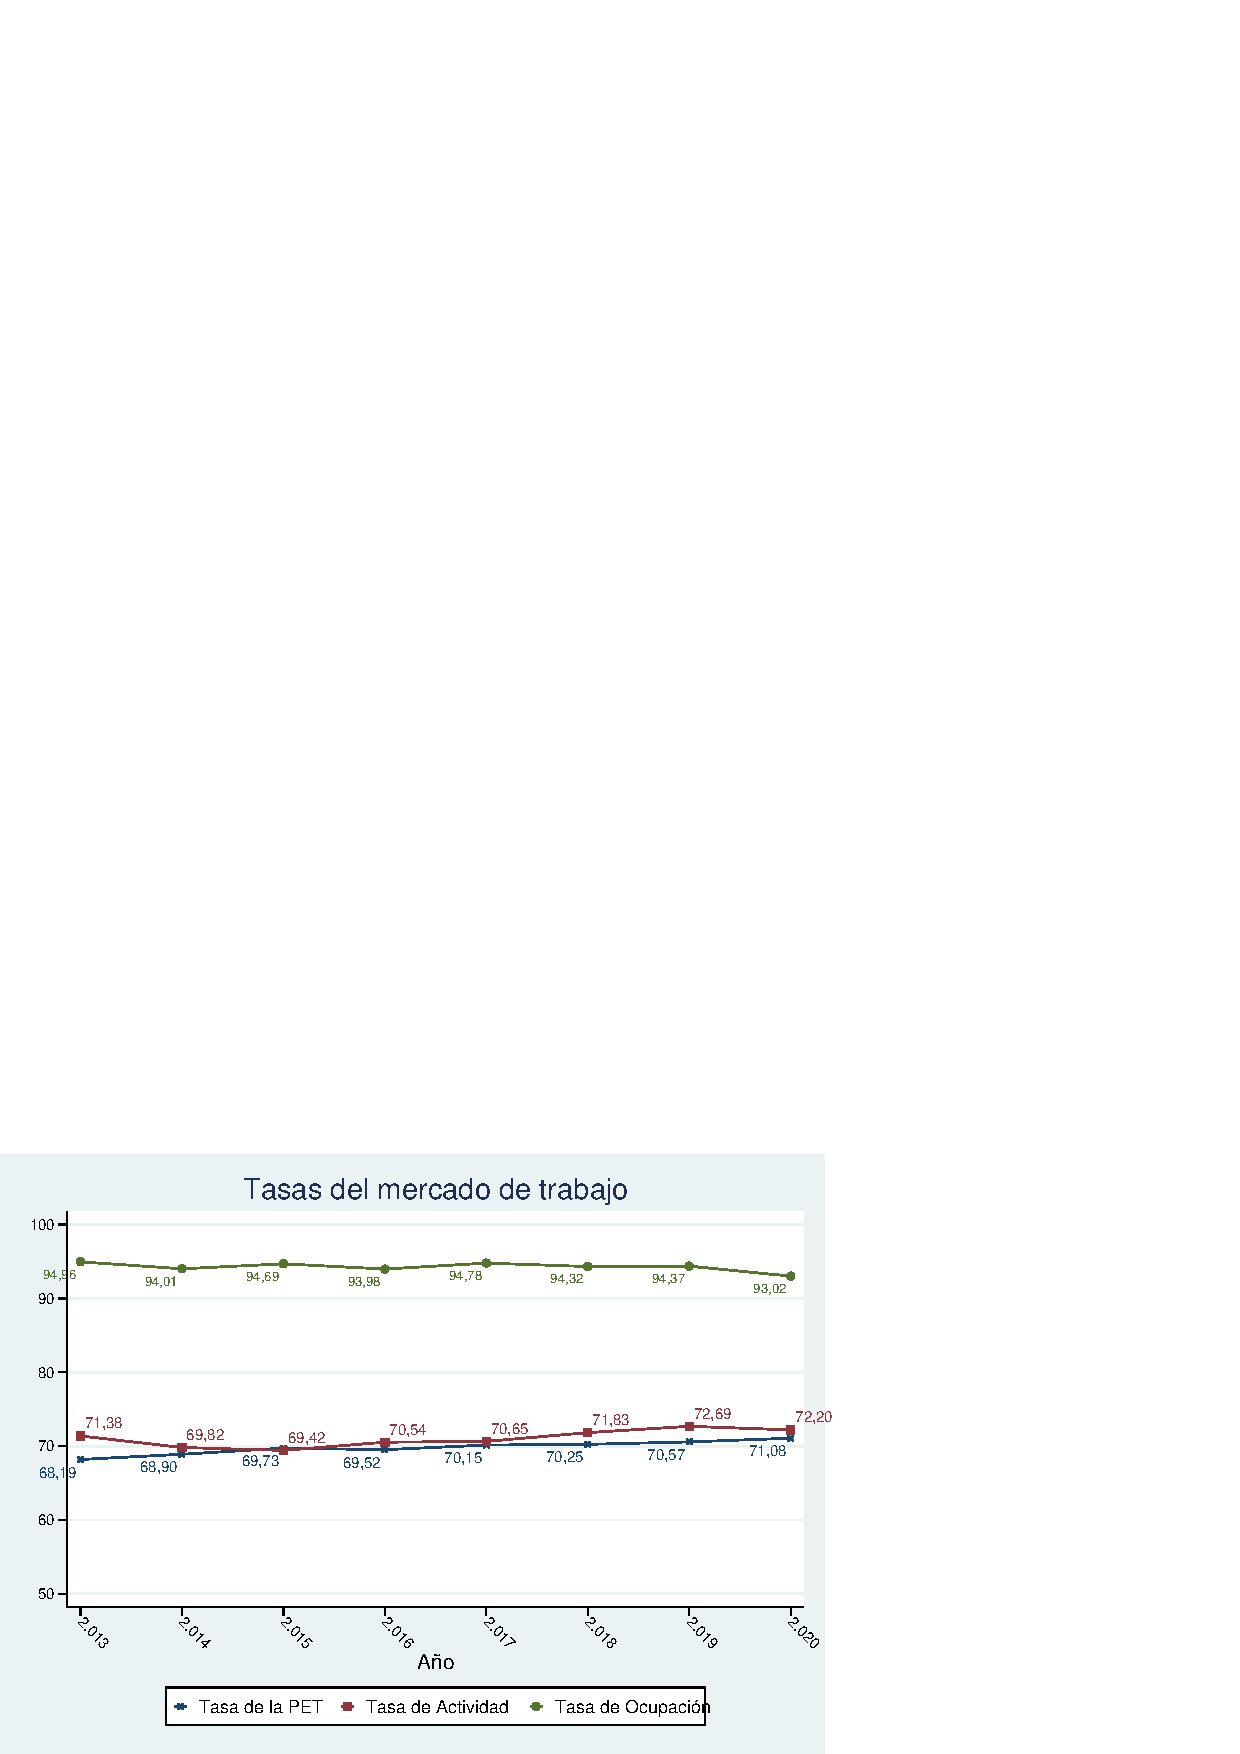
\includegraphics[scale=0.55]{EPH_tasas_peaa.png}
                                    \item \footnotesize Fuente : Instituto Nacional de Estadística.
                                    \item \footnotesize Nota : Tasa de la Población en Edad de Trabajar=PET/PT, Tasa de Actividad=PEA/PET, Tasa de Ocupación=PO/PEA
                    \end{center}
\end{figure}

La participación de la mujer paraguaya en el mercado laboral ha
aumentado en la última década. En la Figura 12 se observa el
comportamiento de la tasa de ocupación por sexo y por tramos de edad.

\begin{figure}[H]
\begin{center}
                    \caption{Evolución de la Tasa de Actividad y de Ocupación por año, según sexo}
                    \includegraphics[scale=0.55]{EPH_tasas_sexo_ocup_act.png}
                                    \item \footnotesize Fuente : Instituto Nacional de Estadística.
                                    \item \footnotesize Nota : Tasa de Ocupación=PO/PEA
                    \end{center}
\end{figure}

\begin{figure}[H]
\begin{center}
                    \caption{Tasas de Actividad y de Ocupación por tramos de edad, según sexo (Año 2020)}
                    \includegraphics[scale=0.55]{EPH_tasasgq_ocupacion_actividad.png}
                                    \item \footnotesize Fuente : Instituto Nacional de Estadística.
                                    \item \footnotesize Nota : Tasa de Ocupación=PO/PEA
                    \end{center}
\end{figure}

La Tasa de Actividad para el año 2020 desagregada por sexo, muestra que
del total de hombres en edad de trabajar un 84,5\% participa en el
mercado laboral, mientras que del total de mujeres en edad de trabajar
un 60,4\% participa en el mercado laboral.

En la distribución de la tasa por sexo según tramos de edad, las curvas
presentan el siguiente comportamiento: valores bajos para los tramos en
los cuales las personas asisten a la escuela/universidad, valores altos
para edades intermedias y baja partic ipación en las edades de retiro y
vejez.

Cabe destacar que, la Tasa de Actividad de las mujeres es inferior a la
de los hombres en todos los tramos etarios observados. En el caso de los
hombres, éstos poseen prácticamente una participación total (cercana al
100\%) en los grupos de edad compren didos entre los 30 - 49 años.

\subsubsection{Asalarización}

Cuando se analiza la Población Activa Ocupada, la segmentación de los
trabajadores según tipo de ocupación indica que el 37,6\% de los mismos
corresponden a mano de obra independiente (cuenta propia y empleador o
patrón). El 54,6\% se encuentra en rela ción de dependencia
clasificándose en Privado 37,9\%, Público 9,9\% y Doméstico 6,9\%. Y el
restante 7,8\% pertenece a la categoría de trabajadores familiares no
remunerados.

La importancia de conocer la relación laboral del trabajador,
\textit{"dependiente / independiente"} o \textit{"publico / privado"},
radica en que, el ámbito de obligatoriedad para aportar al Sistema de
Jubilaciones y Pensiones del IPS se restringe al\\
textit\{``Empleado / Obrero Privado''\} y al
\textit{"Empleado Doméstico \footnote{Clasificación de Categoría Ocupacional utilizada por la EPH del INE, corresponde al tipo de relación de dependencia en el trabajo con la entidad empleadora. Se distinguen den
tro de este tipo de relación: al patrón o socio activo, trabajador por cuenta propia, empleado u obrero público, empleado u obrero de empresa privada, servicio doméstico (asalariado) y trabajador familiar no remunerado.}"}.

\begin{table}[H]
\begin{center}
\scriptsize
\caption{\bf{Población por categoría de ocupación}}
\begin{tabular}{l|rrrrrr}
\begin{tabular}{lllllllll}
\cline{1-9}
\multicolumn{1}{c}{} &
  \multicolumn{8}{|c}{Año} \\
\multicolumn{1}{c}{} &
  \multicolumn{1}{|r}{2013} &
  \multicolumn{1}{r}{2014} &
  \multicolumn{1}{r}{2015} &
  \multicolumn{1}{r}{2016} &
  \multicolumn{1}{r}{2017} &
  \multicolumn{1}{r}{2018} &
  \multicolumn{1}{r}{2019} &
  \multicolumn{1}{r}{2020} \\
\cline{1-9}
\multicolumn{1}{l}{Categoría de Ocupación} &
  \multicolumn{1}{|r}{} &
  \multicolumn{1}{r}{} &
  \multicolumn{1}{r}{} &
  \multicolumn{1}{r}{} &
  \multicolumn{1}{r}{} &
  \multicolumn{1}{r}{} &
  \multicolumn{1}{r}{} &
  \multicolumn{1}{r}{} \\
\multicolumn{1}{l}{\hspace{1em}Empleado / obrero público} &
  \multicolumn{1}{|r}{334.482} &
  \multicolumn{1}{r}{303.628} &
  \multicolumn{1}{r}{348.234} &
  \multicolumn{1}{r}{314.055} &
  \multicolumn{1}{r}{295.901} &
  \multicolumn{1}{r}{340.031} &
  \multicolumn{1}{r}{347.965} &
  \multicolumn{1}{r}{337.401} \\
\multicolumn{1}{l}{\hspace{1em}Empleado / obrero privado} &
  \multicolumn{1}{|r}{1.111.782} &
  \multicolumn{1}{r}{1.183.150} &
  \multicolumn{1}{r}{1.173.650} &
  \multicolumn{1}{r}{1.214.963} &
  \multicolumn{1}{r}{1.275.933} &
  \multicolumn{1}{r}{1.297.794} &
  \multicolumn{1}{r}{1.337.879} &
  \multicolumn{1}{r}{1.295.107} \\
\multicolumn{1}{l}{\hspace{1em}Empleador o patrón} &
  \multicolumn{1}{|r}{193.498} &
  \multicolumn{1}{r}{194.529} &
  \multicolumn{1}{r}{147.142} &
  \multicolumn{1}{r}{159.379} &
  \multicolumn{1}{r}{172.382} &
  \multicolumn{1}{r}{178.991} &
  \multicolumn{1}{r}{181.801} &
  \multicolumn{1}{r}{162.522} \\
\multicolumn{1}{l}{\hspace{1em}Trabajador por cuenta propia} &
  \multicolumn{1}{|r}{934.893} &
  \multicolumn{1}{r}{923.492} &
  \multicolumn{1}{r}{930.815} &
  \multicolumn{1}{r}{985.764} &
  \multicolumn{1}{r}{1.004.297} &
  \multicolumn{1}{r}{1.006.739} &
  \multicolumn{1}{r}{1.047.378} &
  \multicolumn{1}{r}{1.122.778} \\
\multicolumn{1}{l}{\hspace{1em}Trabajador familiar no remunerado} &
  \multicolumn{1}{|r}{199.911} &
  \multicolumn{1}{r}{164.320} &
  \multicolumn{1}{r}{248.157} &
  \multicolumn{1}{r}{235.602} &
  \multicolumn{1}{r}{240.814} &
  \multicolumn{1}{r}{243.886} &
  \multicolumn{1}{r}{245.759} &
  \multicolumn{1}{r}{268.295} \\
\multicolumn{1}{l}{\hspace{1em}Empleado doméstico} &
  \multicolumn{1}{|r}{220.529} &
  \multicolumn{1}{r}{207.382} &
  \multicolumn{1}{r}{213.300} &
  \multicolumn{1}{r}{211.684} &
  \multicolumn{1}{r}{237.093} &
  \multicolumn{1}{r}{249.868} &
  \multicolumn{1}{r}{259.633} &
  \multicolumn{1}{r}{235.333} \\
\multicolumn{1}{l}{\hspace{1em}NR} &
  \multicolumn{1}{|r}{2.520} &
  \multicolumn{1}{r}{361} &
  \multicolumn{1}{r}{82} &
  \multicolumn{1}{r}{1.300} &
  \multicolumn{1}{r}{2.216} &
  \multicolumn{1}{r}{466} &
  \multicolumn{1}{r}{1.916} &
  \multicolumn{1}{r}{} \\
\multicolumn{1}{l}{\hspace{1em}Total} &
  \multicolumn{1}{|r}{2.997.615} &
  \multicolumn{1}{r}{2.976.862} &
  \multicolumn{1}{r}{3.061.380} &
  \multicolumn{1}{r}{3.122.747} &
  \multicolumn{1}{r}{3.228.636} &
  \multicolumn{1}{r}{3.317.775} &
  \multicolumn{1}{r}{3.422.331} &
  \multicolumn{1}{r}{3.421.436} \\
\cline{1-9}
\end{tabular}

\end{tabular}
                    \item \footnotesize Fuente : Encuesta Permanente de Hogares. 
                    \item \footnotesize Nota : Trabajadores ocupados mayores de 14 años.
\end{center}
\end{table}

\begin{table}[H]
\begin{center}
\scriptsize
\caption{\bf{Población por categoría de ocupación (en porcentaje). Periodo 2013-2020}}
\begin{tabular}{l|rrrrrr}
\begin{tabular}{lllllllll}
\cline{1-9}
\multicolumn{1}{c}{} &
  \multicolumn{8}{|c}{Año} \\
\multicolumn{1}{c}{} &
  \multicolumn{1}{|r}{2013} &
  \multicolumn{1}{r}{2014} &
  \multicolumn{1}{r}{2015} &
  \multicolumn{1}{r}{2016} &
  \multicolumn{1}{r}{2017} &
  \multicolumn{1}{r}{2018} &
  \multicolumn{1}{r}{2019} &
  \multicolumn{1}{r}{2020} \\
\cline{1-9}
\multicolumn{1}{l}{Categoría de Ocupación} &
  \multicolumn{1}{|r}{} &
  \multicolumn{1}{r}{} &
  \multicolumn{1}{r}{} &
  \multicolumn{1}{r}{} &
  \multicolumn{1}{r}{} &
  \multicolumn{1}{r}{} &
  \multicolumn{1}{r}{} &
  \multicolumn{1}{r}{} \\
\multicolumn{1}{l}{\hspace{1em}Empleado / obrero público} &
  \multicolumn{1}{|r}{11,16} &
  \multicolumn{1}{r}{10,20} &
  \multicolumn{1}{r}{11,38} &
  \multicolumn{1}{r}{10,06} &
  \multicolumn{1}{r}{9,16} &
  \multicolumn{1}{r}{10,25} &
  \multicolumn{1}{r}{10,17} &
  \multicolumn{1}{r}{9,86} \\
\multicolumn{1}{l}{\hspace{1em}Empleado / obrero privado} &
  \multicolumn{1}{|r}{37,09} &
  \multicolumn{1}{r}{39,74} &
  \multicolumn{1}{r}{38,34} &
  \multicolumn{1}{r}{38,91} &
  \multicolumn{1}{r}{39,52} &
  \multicolumn{1}{r}{39,12} &
  \multicolumn{1}{r}{39,09} &
  \multicolumn{1}{r}{37,85} \\
\multicolumn{1}{l}{\hspace{1em}Empleador o patrón} &
  \multicolumn{1}{|r}{6,46} &
  \multicolumn{1}{r}{6,53} &
  \multicolumn{1}{r}{4,81} &
  \multicolumn{1}{r}{5,10} &
  \multicolumn{1}{r}{5,34} &
  \multicolumn{1}{r}{5,39} &
  \multicolumn{1}{r}{5,31} &
  \multicolumn{1}{r}{4,75} \\
\multicolumn{1}{l}{\hspace{1em}Trabajador por cuenta propia} &
  \multicolumn{1}{|r}{31,19} &
  \multicolumn{1}{r}{31,02} &
  \multicolumn{1}{r}{30,41} &
  \multicolumn{1}{r}{31,57} &
  \multicolumn{1}{r}{31,11} &
  \multicolumn{1}{r}{30,34} &
  \multicolumn{1}{r}{30,60} &
  \multicolumn{1}{r}{32,82} \\
\multicolumn{1}{l}{\hspace{1em}Trabajador familiar no remunerado} &
  \multicolumn{1}{|r}{6,67} &
  \multicolumn{1}{r}{5,52} &
  \multicolumn{1}{r}{8,11} &
  \multicolumn{1}{r}{7,54} &
  \multicolumn{1}{r}{7,46} &
  \multicolumn{1}{r}{7,35} &
  \multicolumn{1}{r}{7,18} &
  \multicolumn{1}{r}{7,84} \\
\multicolumn{1}{l}{\hspace{1em}Empleado doméstico} &
  \multicolumn{1}{|r}{7,36} &
  \multicolumn{1}{r}{6,97} &
  \multicolumn{1}{r}{6,97} &
  \multicolumn{1}{r}{6,78} &
  \multicolumn{1}{r}{7,34} &
  \multicolumn{1}{r}{7,53} &
  \multicolumn{1}{r}{7,59} &
  \multicolumn{1}{r}{6,88} \\
\multicolumn{1}{l}{\hspace{1em}NR} &
  \multicolumn{1}{|r}{0,08} &
  \multicolumn{1}{r}{0,01} &
  \multicolumn{1}{r}{0,00} &
  \multicolumn{1}{r}{0,04} &
  \multicolumn{1}{r}{0,07} &
  \multicolumn{1}{r}{0,01} &
  \multicolumn{1}{r}{0,06} &
  \multicolumn{1}{r}{} \\
\multicolumn{1}{l}{\hspace{1em}Total} &
  \multicolumn{1}{|r}{100,00} &
  \multicolumn{1}{r}{100,00} &
  \multicolumn{1}{r}{100,00} &
  \multicolumn{1}{r}{100,00} &
  \multicolumn{1}{r}{100,00} &
  \multicolumn{1}{r}{100,00} &
  \multicolumn{1}{r}{100,00} &
  \multicolumn{1}{r}{100,00} \\
\cline{1-9}
\end{tabular}

\end{tabular}
                    \item \footnotesize Fuente : Encuesta Permanente de Hogares. 
                    \item \footnotesize Nota : Trabajadores ocupados mayores de 14 años.
\end{center}
\end{table}

En cuanto a las tendencias, se puede ver que la distribución de los
porcentajes de trabajadores por tipo de ocupación es similar en los
últimos 8 años.

El sector privado ha tenido un aumento sostenido entre los años 2013 y
2019, pasando de un valor aproximado de 37,1\% a un valor de 39,1\%.
Para el año 2020 esta proporción disminuyó levemente alcanzando un valor
de 37,9\%.

Por otra parte, el sector de los empleados por cuenta propia ha tenido
un aumento, pasando de un valor de 31,2\% en el año 2013 a un valor de
32,8\% para el año 2020. Las demás categorías no han presentado
variaciones importantes.

\begin{figure}[H]
\begin{center}
                    \caption{Evolución de la cantidad de trabajadores por categoría de ocupación. Periodo 2013-2020}
                    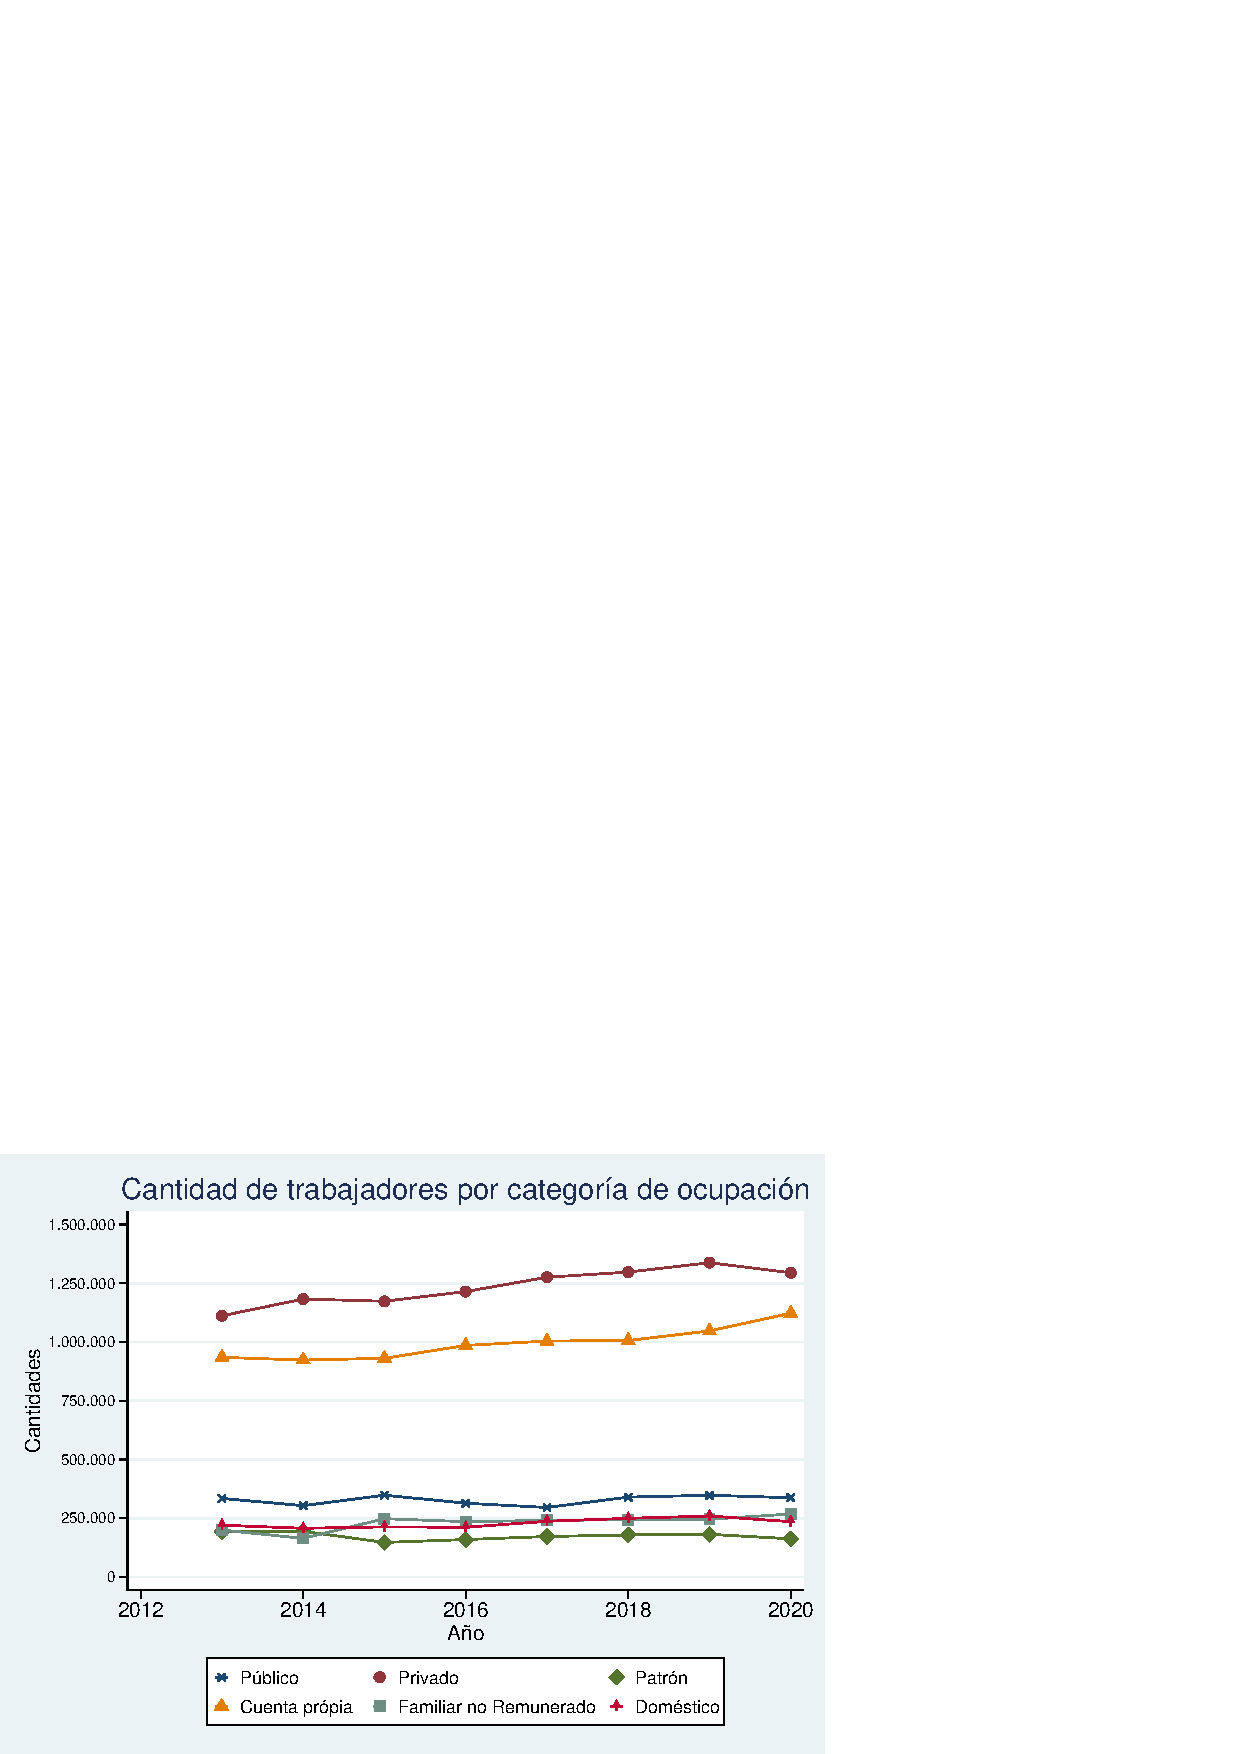
\includegraphics[scale=0.55]{EPH_catepea.png}
                                    \item \footnotesize Fuente : Encuesta Permanente de Hogares.
                                    %\item \footnotesize Nota : 
                    \end{center}
\end{figure}

\newpage
\begin{verbatim}
      . set graph on

      . //ON
\end{verbatim}

\subsection{Estadísticas de familia}\subsubsection{Proporción de casados y edad promedio de la esposa del asegurado titular}

En esta sección se clasifica al asegurado titular del IPS bajo las
siguientes condiciones:

\begin{itemize}
\item si tiene Seguro de Salud del IPS donde es el titular o,
\item si es cotizante al IPS o,
\item si cobra una jubilación y tiene seguro de IPS como jubilado o familiar del jubilado.
\end{itemize}

Por otra parte, es hijo/a dependiente de un asegurado titular del IPS si
tiene menos de 18 años de edad.

Un dato importante a la hora de realizar las proyecciones es la
proporción de casados, de manera a estimar la cantidad de potenciales
pensionados. En ese sentido, el 84\% de los jubilados de entre 60 y 69
años de edad están casados, poseen en promedio 2 (1,74) hijos y la edad
promedio de la esposa es de 66 años.

\begin{table}[H]
\begin{center}
\scriptsize
\caption{\bf{Características de la familia del trabajador asegurado titular del IPS}}
\begin{tabular}{l|rrrrrrrrrrrrrr}
\begin{tabular}{llllllllll}
\cline{1-10}
\multicolumn{1}{c}{} &
  \multicolumn{9}{|c}{Edad quinquenal} \\
\multicolumn{1}{c}{} &
  \multicolumn{1}{|r}{10 a 19} &
  \multicolumn{1}{r}{20 a 29} &
  \multicolumn{1}{r}{30 a 39} &
  \multicolumn{1}{r}{40 a 49} &
  \multicolumn{1}{r}{50 a 59} &
  \multicolumn{1}{r}{60 a 69} &
  \multicolumn{1}{r}{70 a 79} &
  \multicolumn{1}{r}{80 y más} &
  \multicolumn{1}{r}{Total} \\
\cline{1-10}
\multicolumn{1}{l}{Sexo} &
  \multicolumn{1}{|r}{} &
  \multicolumn{1}{r}{} &
  \multicolumn{1}{r}{} &
  \multicolumn{1}{r}{} &
  \multicolumn{1}{r}{} &
  \multicolumn{1}{r}{} &
  \multicolumn{1}{r}{} &
  \multicolumn{1}{r}{} &
  \multicolumn{1}{r}{} \\
\multicolumn{1}{l}{\hspace{1em}Hombres} &
  \multicolumn{1}{|r}{} &
  \multicolumn{1}{r}{} &
  \multicolumn{1}{r}{} &
  \multicolumn{1}{r}{} &
  \multicolumn{1}{r}{} &
  \multicolumn{1}{r}{} &
  \multicolumn{1}{r}{} &
  \multicolumn{1}{r}{} &
  \multicolumn{1}{r}{} \\
\multicolumn{1}{l}{\hspace{2em}Proporción de Casados/as} &
  \multicolumn{1}{|r}{.} &
  \multicolumn{1}{r}{0,44} &
  \multicolumn{1}{r}{0,81} &
  \multicolumn{1}{r}{0,87} &
  \multicolumn{1}{r}{0,88} &
  \multicolumn{1}{r}{0,84} &
  \multicolumn{1}{r}{0,85} &
  \multicolumn{1}{r}{0,59} &
  \multicolumn{1}{r}{0,88} \\
\multicolumn{1}{l}{\hspace{2em}Edad promedio de la esposa/o} &
  \multicolumn{1}{|r}{.} &
  \multicolumn{1}{r}{21,81} &
  \multicolumn{1}{r}{29,74} &
  \multicolumn{1}{r}{38,07} &
  \multicolumn{1}{r}{47,24} &
  \multicolumn{1}{r}{55,80} &
  \multicolumn{1}{r}{66,69} &
  \multicolumn{1}{r}{72,83} &
  \multicolumn{1}{r}{72,83} \\
\multicolumn{1}{l}{\hspace{2em}Nro promedio de hijos/as} &
  \multicolumn{1}{|r}{1,62} &
  \multicolumn{1}{r}{1,61} &
  \multicolumn{1}{r}{1,93} &
  \multicolumn{1}{r}{2,42} &
  \multicolumn{1}{r}{2,37} &
  \multicolumn{1}{r}{1,74} &
  \multicolumn{1}{r}{.} &
  \multicolumn{1}{r}{.} &
  \multicolumn{1}{r}{2,42} \\
\multicolumn{1}{l}{\hspace{2em}Edad promedio del hijo/a} &
  \multicolumn{1}{|r}{3,52} &
  \multicolumn{1}{r}{3,83} &
  \multicolumn{1}{r}{6,45} &
  \multicolumn{1}{r}{10,32} &
  \multicolumn{1}{r}{11,43} &
  \multicolumn{1}{r}{11,43} &
  \multicolumn{1}{r}{.} &
  \multicolumn{1}{r}{.} &
  \multicolumn{1}{r}{11,43} \\
\multicolumn{1}{l}{\hspace{1em}Mujeres} &
  \multicolumn{1}{|r}{} &
  \multicolumn{1}{r}{} &
  \multicolumn{1}{r}{} &
  \multicolumn{1}{r}{} &
  \multicolumn{1}{r}{} &
  \multicolumn{1}{r}{} &
  \multicolumn{1}{r}{} &
  \multicolumn{1}{r}{} &
  \multicolumn{1}{r}{} \\
\multicolumn{1}{l}{\hspace{2em}Proporción de Casados/as} &
  \multicolumn{1}{|r}{.} &
  \multicolumn{1}{r}{0,39} &
  \multicolumn{1}{r}{0,68} &
  \multicolumn{1}{r}{0,70} &
  \multicolumn{1}{r}{0,68} &
  \multicolumn{1}{r}{0,62} &
  \multicolumn{1}{r}{0,48} &
  \multicolumn{1}{r}{0,25} &
  \multicolumn{1}{r}{0,70} \\
\multicolumn{1}{l}{\hspace{2em}Edad promedio de la esposa/o} &
  \multicolumn{1}{|r}{.} &
  \multicolumn{1}{r}{25,88} &
  \multicolumn{1}{r}{34,12} &
  \multicolumn{1}{r}{43,94} &
  \multicolumn{1}{r}{53,86} &
  \multicolumn{1}{r}{65,71} &
  \multicolumn{1}{r}{71,56} &
  \multicolumn{1}{r}{81,44} &
  \multicolumn{1}{r}{81,44} \\
\multicolumn{1}{l}{\hspace{2em}Nro promedio de hijos/as} &
  \multicolumn{1}{|r}{.} &
  \multicolumn{1}{r}{1,50} &
  \multicolumn{1}{r}{1,99} &
  \multicolumn{1}{r}{2,31} &
  \multicolumn{1}{r}{1,63} &
  \multicolumn{1}{r}{.} &
  \multicolumn{1}{r}{.} &
  \multicolumn{1}{r}{.} &
  \multicolumn{1}{r}{2,31} \\
\multicolumn{1}{l}{\hspace{2em}Edad promedio del hijo/a} &
  \multicolumn{1}{|r}{.} &
  \multicolumn{1}{r}{4,00} &
  \multicolumn{1}{r}{7,34} &
  \multicolumn{1}{r}{11,42} &
  \multicolumn{1}{r}{13,25} &
  \multicolumn{1}{r}{.} &
  \multicolumn{1}{r}{.} &
  \multicolumn{1}{r}{.} &
  \multicolumn{1}{r}{13,25} \\
\multicolumn{1}{l}{\hspace{1em}Total} &
  \multicolumn{1}{|r}{} &
  \multicolumn{1}{r}{} &
  \multicolumn{1}{r}{} &
  \multicolumn{1}{r}{} &
  \multicolumn{1}{r}{} &
  \multicolumn{1}{r}{} &
  \multicolumn{1}{r}{} &
  \multicolumn{1}{r}{} &
  \multicolumn{1}{r}{} \\
\multicolumn{1}{l}{\hspace{2em}Proporción de Casados/as} &
  \multicolumn{1}{|r}{.} &
  \multicolumn{1}{r}{0,44} &
  \multicolumn{1}{r}{0,81} &
  \multicolumn{1}{r}{0,87} &
  \multicolumn{1}{r}{0,88} &
  \multicolumn{1}{r}{0,84} &
  \multicolumn{1}{r}{0,85} &
  \multicolumn{1}{r}{0,59} &
  \multicolumn{1}{r}{0,88} \\
\multicolumn{1}{l}{\hspace{2em}Edad promedio de la esposa/o} &
  \multicolumn{1}{|r}{.} &
  \multicolumn{1}{r}{25,88} &
  \multicolumn{1}{r}{34,12} &
  \multicolumn{1}{r}{43,94} &
  \multicolumn{1}{r}{53,86} &
  \multicolumn{1}{r}{65,71} &
  \multicolumn{1}{r}{71,56} &
  \multicolumn{1}{r}{81,44} &
  \multicolumn{1}{r}{81,44} \\
\multicolumn{1}{l}{\hspace{2em}Nro promedio de hijos/as} &
  \multicolumn{1}{|r}{1,62} &
  \multicolumn{1}{r}{1,61} &
  \multicolumn{1}{r}{1,99} &
  \multicolumn{1}{r}{2,42} &
  \multicolumn{1}{r}{2,37} &
  \multicolumn{1}{r}{1,74} &
  \multicolumn{1}{r}{.} &
  \multicolumn{1}{r}{.} &
  \multicolumn{1}{r}{2,42} \\
\multicolumn{1}{l}{\hspace{2em}Edad promedio del hijo/a} &
  \multicolumn{1}{|r}{3,52} &
  \multicolumn{1}{r}{4,00} &
  \multicolumn{1}{r}{7,34} &
  \multicolumn{1}{r}{11,42} &
  \multicolumn{1}{r}{13,25} &
  \multicolumn{1}{r}{11,43} &
  \multicolumn{1}{r}{.} &
  \multicolumn{1}{r}{.} &
  \multicolumn{1}{r}{13,25} \\
\cline{1-10}
\end{tabular}

\end{tabular}
                                    \item \footnotesize Fuente : Encuesta Permanente de Hogares.
                    %\item \footnotesize Nota : Trabajadores ocupados mayores de 14 años.
\end{center}
\end{table}

\begin{figure}[H]
\begin{center}
                    \caption{Proporción de casados por edad y sexo del asegurado titular}
                    \includegraphics[scale=0.35]{EPH_familia_prop_casado.png}
                                    \item \footnotesize Fuente : Encuesta Permanente de Hogares.
                                    \item \footnotesize Nota : 
                    \end{center}
\end{figure}

\begin{figure}[H]
\begin{center}
                    \caption{Edad promedio de la esposa y del esposo por edad y sexo del asegurado titular}
                    \includegraphics[scale=0.35]{EPH_familia_edadmed_esposa.png}
                                    \item \footnotesize Fuente : Encuesta Permanente de Hogares.
                                    \item \footnotesize Nota : 
                    \end{center}
\end{figure}

\subsubsection{Cantidad promedio y edad promedio de los hijos del asegurado titular}

Es hijo/a dependiente de un asegurado titular del IPS si tiene menos de
18 años de edad.

\begin{figure}[H]
\begin{center}
                    \caption{Cantidad promedio de hijos dependientes por edad y sexo del asegurado titular}
                    \includegraphics[scale=0.35]{EPH_familia_nro_prom_hijos.png}
                                    \item \footnotesize Fuente : Encuesta Permanente de Hogares.
                                    \item \footnotesize Nota : 
                    \end{center}
\end{figure}

\begin{figure}[H]
\begin{center}
                    \caption{Edad promedio de los hijos dependientes por edad y sexo del asegurado titular}
                    \includegraphics[scale=0.35]{EPH_familia_edad_prom_hijos.png}
                                    \item \footnotesize Fuente : Encuesta Permanente de Hogares.
                                    \item \footnotesize Nota : 
                    \end{center}
\end{figure}

\newpage
\subsection{Contexto Económico}\subsubsection{Producto Interno Bruto}

El PIB
\footnote{Producto Interno Bruto a precios de comprador, en millones de guaraníes constantes de 2014.}
del Paraguay ha crecido en promedio a un ritmo del 3,5\% anual entre los
años 2009 y 2020, donde se destacan dos picos de crecimiento en los a
ños 2010 y 2013 y dos de contracción de la economía en los años 2009 y
2012. Considerando los últimos 5 años el crecimiento ha sido sostenido y
en torno al 2,3\%.

El PIB del año 2020 da cuenta de un decrecimiento económico del orden
del 0,6\%
\footnote{Anexo Estadístico del Informe Económico del BCP. Departamento de Estadísticas del Sector Real.},
esto concuerda con la declaración de estado de emergencia en todo el
territorio nacional ante la pandemia declarada por la Organización
Mundial de la Salud a causa del COVID-19 o CORONAVIRUS, la cual ha
traído consigo innumerables crisis asociadas, tanto en el ámbito
sanitario como en el económico y social.

\begin{figure}[H]
\begin{center}
                    \caption{PIB a precios corrientes y constantes}
                    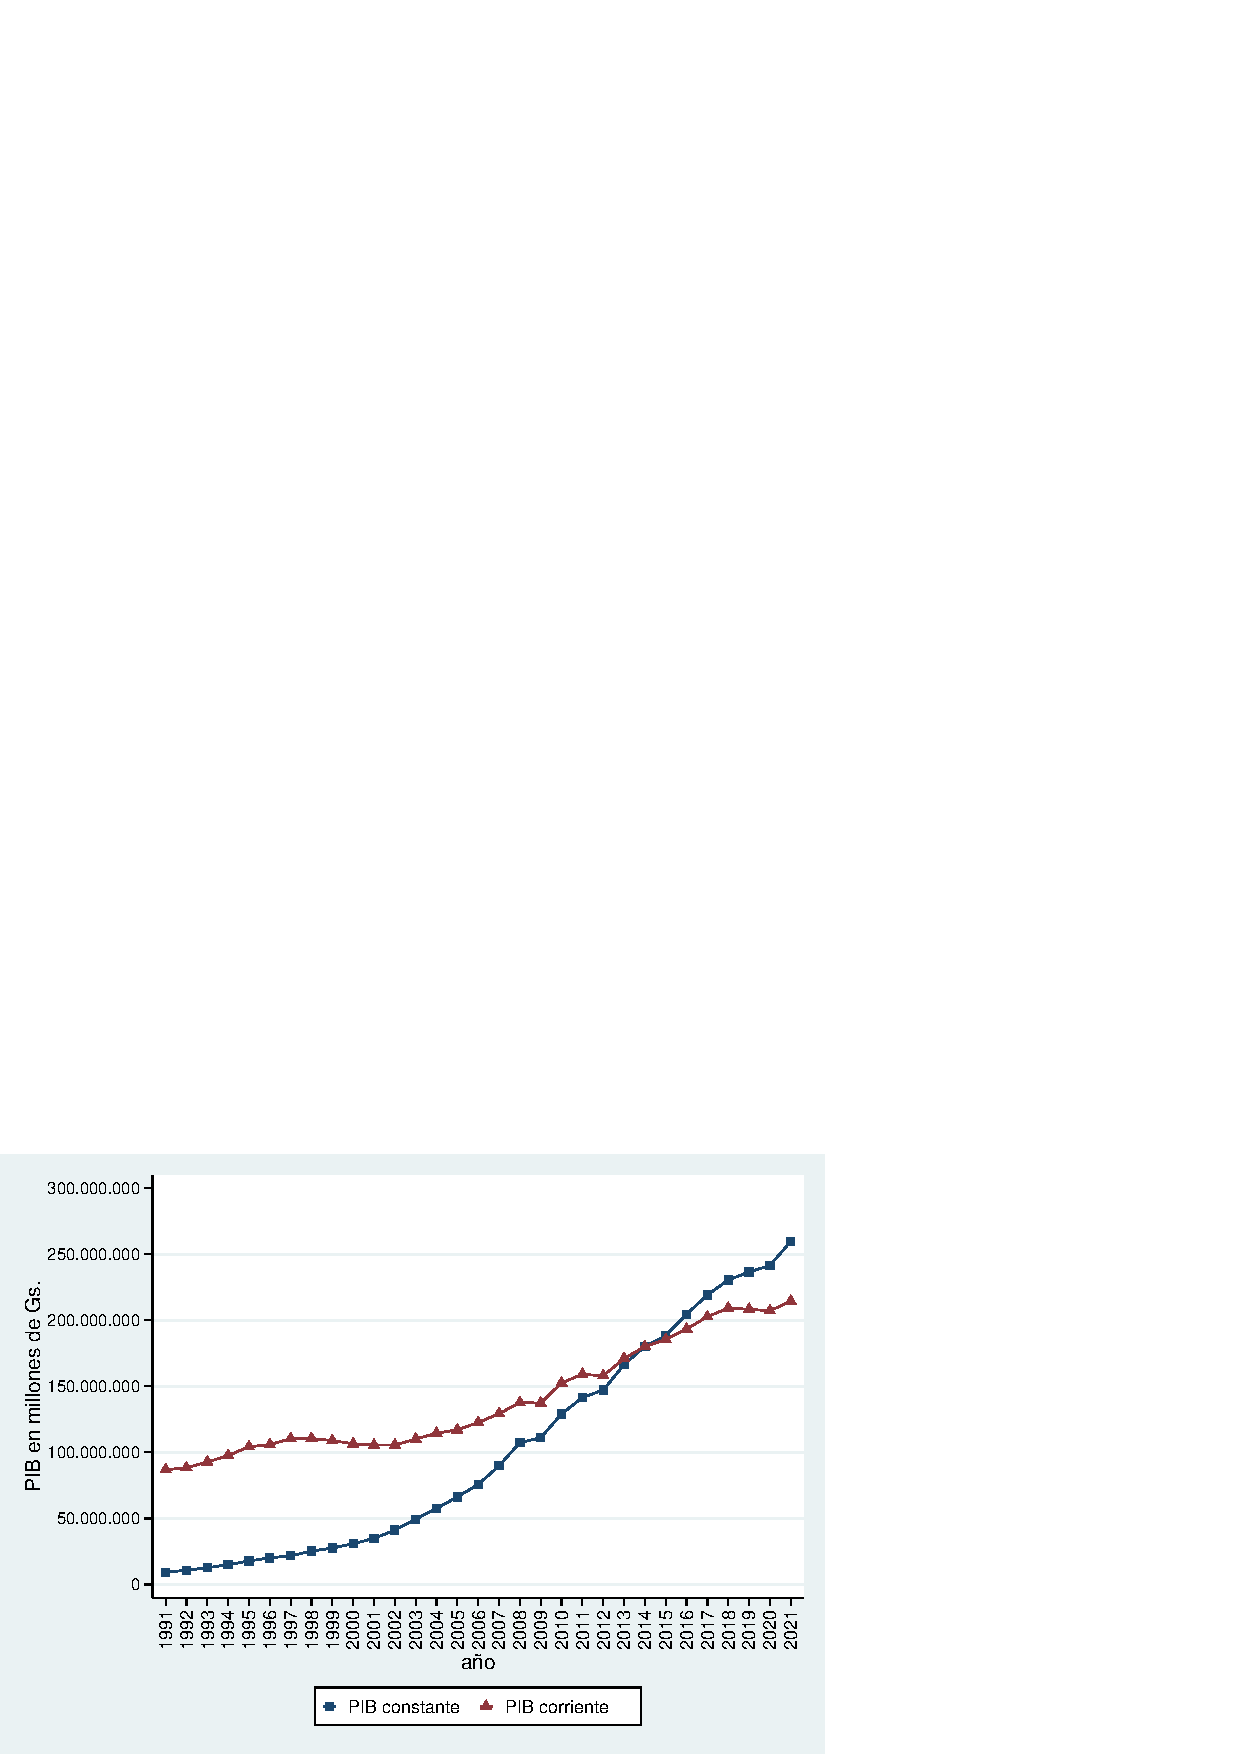
\includegraphics[scale=0.55]{BCP_pib_corr_cte.png}
                                    \item \footnotesize Fuente : Banco Central del Paraguay. 
                                    \item \footnotesize Nota : 
                    \end{center}
\end{figure}

\begin{figure}[H]
\begin{center}
                    \caption{Variación interanual del PIB a precios constantes. Periodo 1991-2021}
                    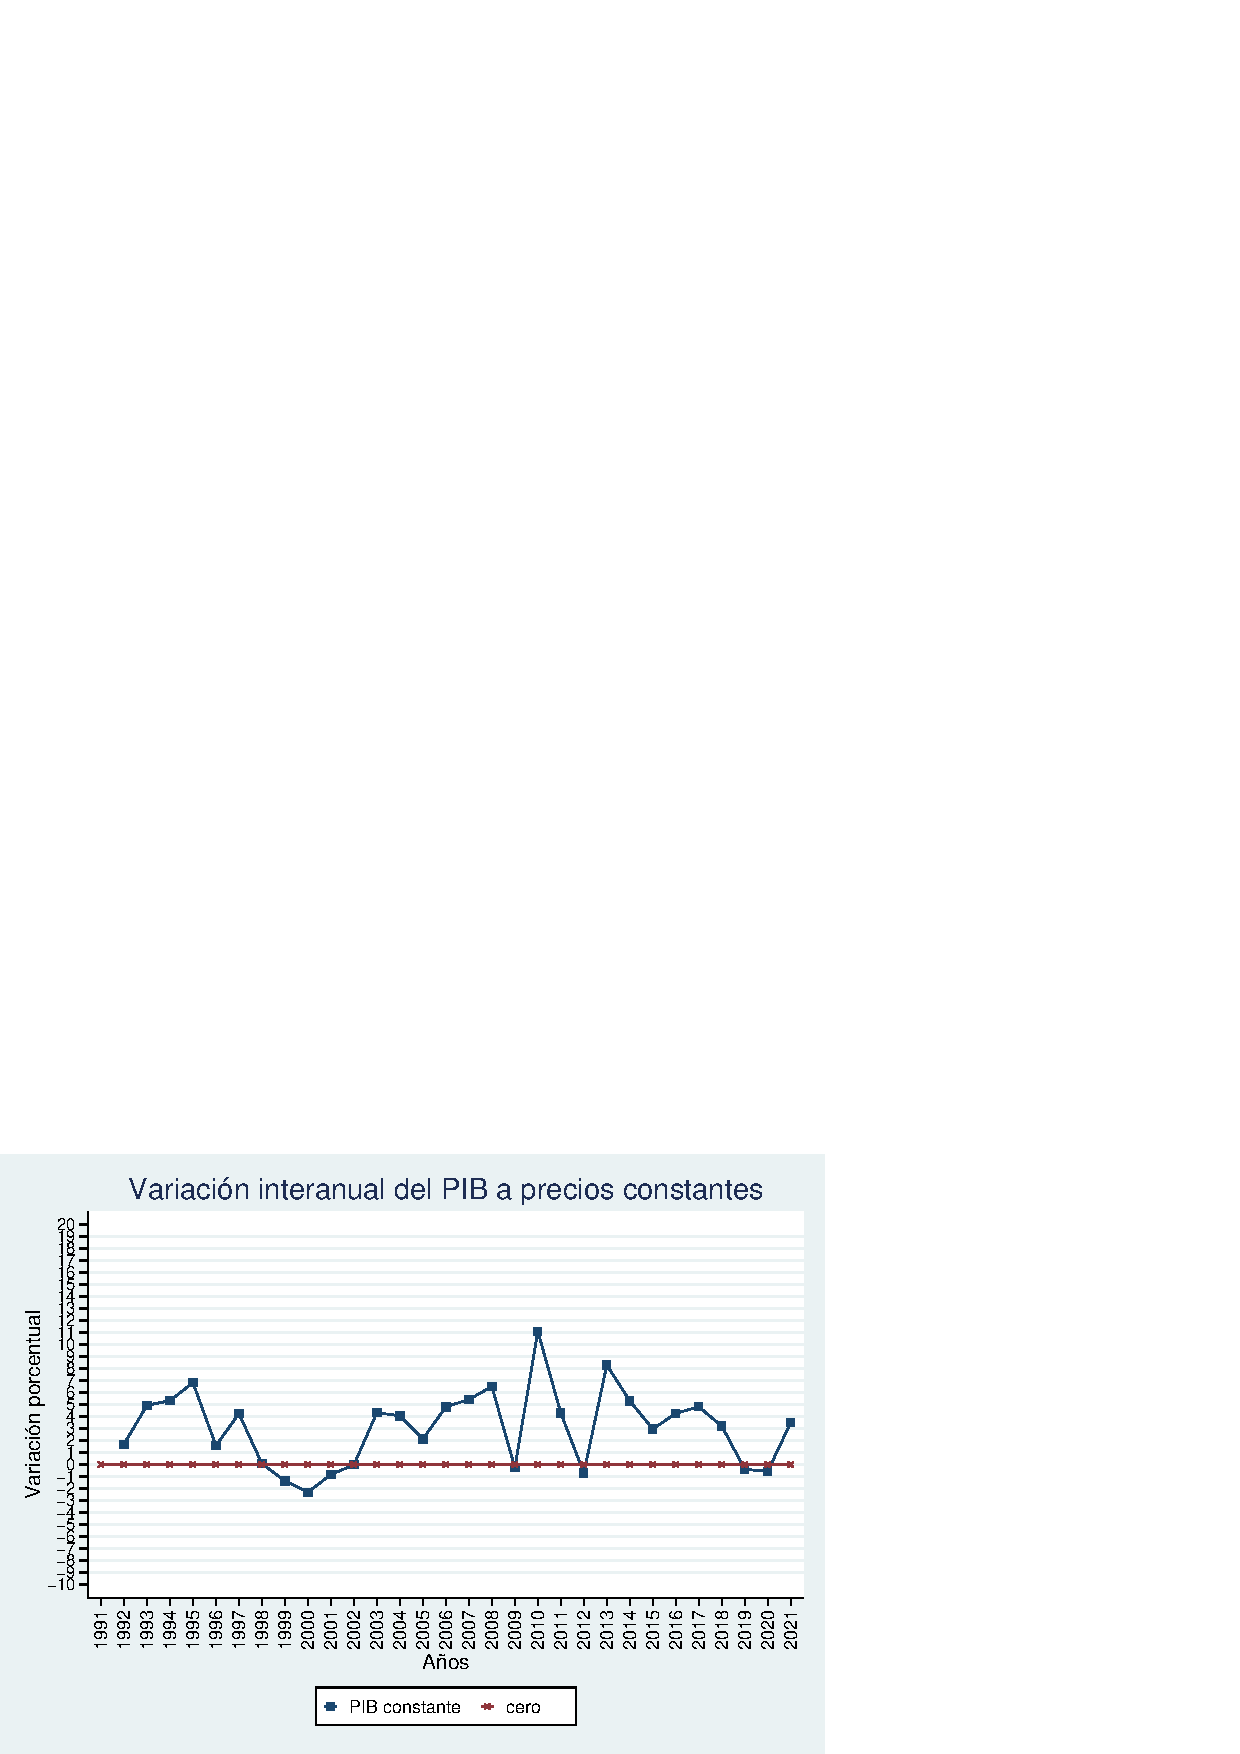
\includegraphics[scale=0.55]{BCP_var_pibcte.png}
                                    \item \footnotesize Fuente : Banco Central del Paraguay. 
                                    %\item \footnotesize Nota : 
                    \end{center}
\end{figure}

\begin{table}[H]
\begin{center}
\scriptsize
\caption{\bf{PIB a precios corrientes y constantes. Periodo 1991-2021}}
\begin{tabular}{l|rrrrrr}
\begin{tabular}{llll}
\cline{1-4}
\multicolumn{1}{c}{} &
  \multicolumn{1}{|r}{PIB\_constantes} &
  \multicolumn{1}{r}{PIB\_corrientes} &
  \multicolumn{1}{r}{Variación del PIB\_contante} \\
\cline{1-4}
\multicolumn{1}{l}{Año} &
  \multicolumn{1}{|r}{} &
  \multicolumn{1}{r}{} &
  \multicolumn{1}{r}{} \\
\multicolumn{1}{l}{\hspace{1em}1991} &
  \multicolumn{1}{|r}{86.864.501,40} &
  \multicolumn{1}{r}{9.255.684,16} &
  \multicolumn{1}{r}{0,00} \\
\multicolumn{1}{l}{\hspace{1em}1992} &
  \multicolumn{1}{|r}{88.338.095,13} &
  \multicolumn{1}{r}{10.738.283,27} &
  \multicolumn{1}{r}{1,70} \\
\multicolumn{1}{l}{\hspace{1em}1993} &
  \multicolumn{1}{|r}{92.698.781,01} &
  \multicolumn{1}{r}{12.645.361,49} &
  \multicolumn{1}{r}{4,94} \\
\multicolumn{1}{l}{\hspace{1em}1994} &
  \multicolumn{1}{|r}{97.628.425,86} &
  \multicolumn{1}{r}{14.992.331,68} &
  \multicolumn{1}{r}{5,32} \\
\multicolumn{1}{l}{\hspace{1em}1995} &
  \multicolumn{1}{|r}{104.289.428,16} &
  \multicolumn{1}{r}{17.789.145,33} &
  \multicolumn{1}{r}{6,82} \\
\multicolumn{1}{l}{\hspace{1em}1996} &
  \multicolumn{1}{|r}{105.930.719,67} &
  \multicolumn{1}{r}{20.132.862,10} &
  \multicolumn{1}{r}{1,57} \\
\multicolumn{1}{l}{\hspace{1em}1997} &
  \multicolumn{1}{|r}{110.424.847,51} &
  \multicolumn{1}{r}{21.702.866,40} &
  \multicolumn{1}{r}{4,24} \\
\multicolumn{1}{l}{\hspace{1em}1998} &
  \multicolumn{1}{|r}{110.499.978,10} &
  \multicolumn{1}{r}{25.248.610,40} &
  \multicolumn{1}{r}{0,07} \\
\multicolumn{1}{l}{\hspace{1em}1999} &
  \multicolumn{1}{|r}{108.990.460,31} &
  \multicolumn{1}{r}{27.563.440,66} &
  \multicolumn{1}{r}{-1,37} \\
\multicolumn{1}{l}{\hspace{1em}2000} &
  \multicolumn{1}{|r}{106.468.267,86} &
  \multicolumn{1}{r}{30.874.087,61} &
  \multicolumn{1}{r}{-2,31} \\
\multicolumn{1}{l}{\hspace{1em}2001} &
  \multicolumn{1}{|r}{105.580.264,25} &
  \multicolumn{1}{r}{34.883.186,50} &
  \multicolumn{1}{r}{-0,83} \\
\multicolumn{1}{l}{\hspace{1em}2002} &
  \multicolumn{1}{|r}{105.557.665,43} &
  \multicolumn{1}{r}{41.135.696,94} &
  \multicolumn{1}{r}{-0,02} \\
\multicolumn{1}{l}{\hspace{1em}2003} &
  \multicolumn{1}{|r}{110.118.543,49} &
  \multicolumn{1}{r}{49.411.959,70} &
  \multicolumn{1}{r}{4,32} \\
\multicolumn{1}{l}{\hspace{1em}2004} &
  \multicolumn{1}{|r}{114.586.513,50} &
  \multicolumn{1}{r}{57.501.991,73} &
  \multicolumn{1}{r}{4,06} \\
\multicolumn{1}{l}{\hspace{1em}2005} &
  \multicolumn{1}{|r}{117.031.206,07} &
  \multicolumn{1}{r}{66.335.828,41} &
  \multicolumn{1}{r}{2,13} \\
\multicolumn{1}{l}{\hspace{1em}2006} &
  \multicolumn{1}{|r}{122.657.033,30} &
  \multicolumn{1}{r}{75.681.657,80} &
  \multicolumn{1}{r}{4,81} \\
\multicolumn{1}{l}{\hspace{1em}2007} &
  \multicolumn{1}{|r}{129.307.035,07} &
  \multicolumn{1}{r}{89.866.048,80} &
  \multicolumn{1}{r}{5,42} \\
\multicolumn{1}{l}{\hspace{1em}2008} &
  \multicolumn{1}{|r}{137.707.197,80} &
  \multicolumn{1}{r}{107.403.590,63} &
  \multicolumn{1}{r}{6,50} \\
\multicolumn{1}{l}{\hspace{1em}2009} &
  \multicolumn{1}{|r}{137.347.592,90} &
  \multicolumn{1}{r}{111.030.933,59} &
  \multicolumn{1}{r}{-0,26} \\
\multicolumn{1}{l}{\hspace{1em}2010} &
  \multicolumn{1}{|r}{152.586.625,97} &
  \multicolumn{1}{r}{129.092.883,48} &
  \multicolumn{1}{r}{11,10} \\
\multicolumn{1}{l}{\hspace{1em}2011} &
  \multicolumn{1}{|r}{159.127.055,18} &
  \multicolumn{1}{r}{141.486.449,39} &
  \multicolumn{1}{r}{4,29} \\
\multicolumn{1}{l}{\hspace{1em}2012} &
  \multicolumn{1}{|r}{158.000.367,02} &
  \multicolumn{1}{r}{147.225.506,09} &
  \multicolumn{1}{r}{-0,71} \\
\multicolumn{1}{l}{\hspace{1em}2013} &
  \multicolumn{1}{|r}{171.103.458,31} &
  \multicolumn{1}{r}{166.350.805,11} &
  \multicolumn{1}{r}{8,29} \\
\multicolumn{1}{l}{\hspace{1em}2014} &
  \multicolumn{1}{|r}{180.174.060,88} &
  \multicolumn{1}{r}{180.174.060,97} &
  \multicolumn{1}{r}{5,30} \\
\multicolumn{1}{l}{\hspace{1em}2015} &
  \multicolumn{1}{|r}{185.502.081,24} &
  \multicolumn{1}{r}{188.477.326,98} &
  \multicolumn{1}{r}{2,96} \\
\multicolumn{1}{l}{\hspace{1em}2016} &
  \multicolumn{1}{|r}{193.419.357,99} &
  \multicolumn{1}{r}{204.647.273,08} &
  \multicolumn{1}{r}{4,27} \\
\multicolumn{1}{l}{\hspace{1em}2017} &
  \multicolumn{1}{|r}{202.722.981,63} &
  \multicolumn{1}{r}{219.122.277,20} &
  \multicolumn{1}{r}{4,81} \\
\multicolumn{1}{l}{\hspace{1em}2018} &
  \multicolumn{1}{|r}{209.218.733,46} &
  \multicolumn{1}{r}{230.576.477,47} &
  \multicolumn{1}{r}{3,20} \\
\multicolumn{1}{l}{\hspace{1em}2019} &
  \multicolumn{1}{|r}{208.377.977,31} &
  \multicolumn{1}{r}{236.566.703,63} &
  \multicolumn{1}{r}{-0,40} \\
\multicolumn{1}{l}{\hspace{1em}2020} &
  \multicolumn{1}{|r}{207.199.192,58} &
  \multicolumn{1}{r}{241.527.085,72} &
  \multicolumn{1}{r}{-0,57} \\
\multicolumn{1}{l}{\hspace{1em}2021} &
  \multicolumn{1}{|r}{214.451.164,32} &
  \multicolumn{1}{r}{259.745.767,58} &
  \multicolumn{1}{r}{3,50} \\
\cline{1-4}
\end{tabular}

\end{tabular}
                    \item \footnotesize Fuente : Banco Central del Paraguay. 
                    %\item \footnotesize Nota : 
\end{center}
\end{table}

\subsubsection{Inflación}

La
inflación\footnote{Índice de Precios al Consumidor. Base diciembre de 2017=100.}
, en economía, es el aumento generalizado y sostenido de los precios de
los bienes y servicios existentes en el mercado durante un período de
tiempo, y uno de los mecani smos para medir la variación de precios en
el Paraguay es a través del Índice de Precios al Consumidor (IPC) del
Área Metropolitana de Asunción elaborado por el BCP, el cual mide la
evolución de los precios (en promedio) de un conjunto de bienes y servi
cios representativos del gasto de consumo de los hogares (una canasta).

La inflación del año 2020 ha ascendido a 2,2\% por debajo del 2,8\%
registrado en al año 2019. En tanto que la inflación interanual a julio
de 2021 ascendió a 5,2\%, superior a la tasa del 4,5\% registrada en
junio del corriente año \footnote{Informe de
 Inflación (IPC)-Julio 2021.}. Pese a esto, la variación aún se sitúa
dentro del rango objetivo a largo plazo establecido por el BCP de 4\% ±
2\% \footnote{Informe de Política Monetaria (Diciembre/2020)-BCP.}.

\begin{table}[H]
\begin{center}
\scriptsize
\caption{\bf{Evolución del Índice de Precios al Consumidor.}}
\begin{tabular}{l|rrrrrrrrrrrrrrr}
\begin{tabular}{lllllllllllll}
\cline{1-13}
\multicolumn{1}{c}{} &
  \multicolumn{12}{|c}{Mes} \\
\multicolumn{1}{c}{} &
  \multicolumn{1}{|r}{Ene} &
  \multicolumn{1}{r}{Feb} &
  \multicolumn{1}{r}{Mar} &
  \multicolumn{1}{r}{Abr} &
  \multicolumn{1}{r}{May} &
  \multicolumn{1}{r}{Jun} &
  \multicolumn{1}{r}{Jul} &
  \multicolumn{1}{r}{Ago} &
  \multicolumn{1}{r}{Sep} &
  \multicolumn{1}{r}{Oct} &
  \multicolumn{1}{r}{Nov} &
  \multicolumn{1}{r}{Dic} \\
\cline{1-13}
\multicolumn{1}{l}{Año} &
  \multicolumn{1}{|r}{} &
  \multicolumn{1}{r}{} &
  \multicolumn{1}{r}{} &
  \multicolumn{1}{r}{} &
  \multicolumn{1}{r}{} &
  \multicolumn{1}{r}{} &
  \multicolumn{1}{r}{} &
  \multicolumn{1}{r}{} &
  \multicolumn{1}{r}{} &
  \multicolumn{1}{r}{} &
  \multicolumn{1}{r}{} &
  \multicolumn{1}{r}{} \\
\multicolumn{1}{l}{\hspace{1em}2000} &
  \multicolumn{1}{|r}{32,86} &
  \multicolumn{1}{r}{33,33} &
  \multicolumn{1}{r}{34,02} &
  \multicolumn{1}{r}{34,31} &
  \multicolumn{1}{r}{34,44} &
  \multicolumn{1}{r}{34,24} &
  \multicolumn{1}{r}{34,32} &
  \multicolumn{1}{r}{34,54} &
  \multicolumn{1}{r}{35,05} &
  \multicolumn{1}{r}{35,26} &
  \multicolumn{1}{r}{35,39} &
  \multicolumn{1}{r}{35,26} \\
\multicolumn{1}{l}{\hspace{1em}2001} &
  \multicolumn{1}{|r}{35,78} &
  \multicolumn{1}{r}{36,01} &
  \multicolumn{1}{r}{36,67} &
  \multicolumn{1}{r}{36,99} &
  \multicolumn{1}{r}{36,74} &
  \multicolumn{1}{r}{36,52} &
  \multicolumn{1}{r}{36,67} &
  \multicolumn{1}{r}{37,03} &
  \multicolumn{1}{r}{37,29} &
  \multicolumn{1}{r}{37,46} &
  \multicolumn{1}{r}{37,66} &
  \multicolumn{1}{r}{38,21} \\
\multicolumn{1}{l}{\hspace{1em}2002} &
  \multicolumn{1}{|r}{38,54} &
  \multicolumn{1}{r}{38,56} &
  \multicolumn{1}{r}{39,05} &
  \multicolumn{1}{r}{39,24} &
  \multicolumn{1}{r}{39,23} &
  \multicolumn{1}{r}{39,94} &
  \multicolumn{1}{r}{41,02} &
  \multicolumn{1}{r}{41,97} &
  \multicolumn{1}{r}{42,45} &
  \multicolumn{1}{r}{42,63} &
  \multicolumn{1}{r}{43,16} &
  \multicolumn{1}{r}{43,81} \\
\multicolumn{1}{l}{\hspace{1em}2003} &
  \multicolumn{1}{|r}{45,54} &
  \multicolumn{1}{r}{46,35} &
  \multicolumn{1}{r}{46,93} &
  \multicolumn{1}{r}{47,48} &
  \multicolumn{1}{r}{46,92} &
  \multicolumn{1}{r}{46,23} &
  \multicolumn{1}{r}{45,93} &
  \multicolumn{1}{r}{45,82} &
  \multicolumn{1}{r}{45,88} &
  \multicolumn{1}{r}{46,83} &
  \multicolumn{1}{r}{47,45} &
  \multicolumn{1}{r}{47,89} \\
\multicolumn{1}{l}{\hspace{1em}2004} &
  \multicolumn{1}{|r}{48,04} &
  \multicolumn{1}{r}{48,11} &
  \multicolumn{1}{r}{48,33} &
  \multicolumn{1}{r}{48,25} &
  \multicolumn{1}{r}{48,36} &
  \multicolumn{1}{r}{48,79} &
  \multicolumn{1}{r}{48,87} &
  \multicolumn{1}{r}{49,60} &
  \multicolumn{1}{r}{48,94} &
  \multicolumn{1}{r}{48,51} &
  \multicolumn{1}{r}{48,44} &
  \multicolumn{1}{r}{49,24} \\
\multicolumn{1}{l}{\hspace{1em}2005} &
  \multicolumn{1}{|r}{49,58} &
  \multicolumn{1}{r}{49,86} &
  \multicolumn{1}{r}{50,45} &
  \multicolumn{1}{r}{51,08} &
  \multicolumn{1}{r}{51,82} &
  \multicolumn{1}{r}{51,76} &
  \multicolumn{1}{r}{52,00} &
  \multicolumn{1}{r}{51,93} &
  \multicolumn{1}{r}{52,64} &
  \multicolumn{1}{r}{53,49} &
  \multicolumn{1}{r}{54,41} &
  \multicolumn{1}{r}{54,09} \\
\multicolumn{1}{l}{\hspace{1em}2006} &
  \multicolumn{1}{|r}{54,85} &
  \multicolumn{1}{r}{55,45} &
  \multicolumn{1}{r}{56,28} &
  \multicolumn{1}{r}{56,51} &
  \multicolumn{1}{r}{56,35} &
  \multicolumn{1}{r}{56,10} &
  \multicolumn{1}{r}{55,99} &
  \multicolumn{1}{r}{56,10} &
  \multicolumn{1}{r}{57,02} &
  \multicolumn{1}{r}{58,15} &
  \multicolumn{1}{r}{59,25} &
  \multicolumn{1}{r}{60,84} \\
\multicolumn{1}{l}{\hspace{1em}2007} &
  \multicolumn{1}{|r}{60,21} &
  \multicolumn{1}{r}{60,03} &
  \multicolumn{1}{r}{59,46} &
  \multicolumn{1}{r}{60,02} &
  \multicolumn{1}{r}{60,35} &
  \multicolumn{1}{r}{59,94} &
  \multicolumn{1}{r}{60,18} &
  \multicolumn{1}{r}{62,22} &
  \multicolumn{1}{r}{62,78} &
  \multicolumn{1}{r}{65,11} &
  \multicolumn{1}{r}{63,65} &
  \multicolumn{1}{r}{64,47} \\
\multicolumn{1}{l}{\hspace{1em}2008} &
  \multicolumn{1}{|r}{65,51} &
  \multicolumn{1}{r}{66,34} &
  \multicolumn{1}{r}{66,80} &
  \multicolumn{1}{r}{67,31} &
  \multicolumn{1}{r}{67,18} &
  \multicolumn{1}{r}{67,96} &
  \multicolumn{1}{r}{68,28} &
  \multicolumn{1}{r}{68,67} &
  \multicolumn{1}{r}{68,47} &
  \multicolumn{1}{r}{68,67} &
  \multicolumn{1}{r}{68,92} &
  \multicolumn{1}{r}{69,31} \\
\multicolumn{1}{l}{\hspace{1em}2009} &
  \multicolumn{1}{|r}{69,37} &
  \multicolumn{1}{r}{69,18} &
  \multicolumn{1}{r}{69,05} &
  \multicolumn{1}{r}{68,67} &
  \multicolumn{1}{r}{68,67} &
  \multicolumn{1}{r}{69,25} &
  \multicolumn{1}{r}{69,05} &
  \multicolumn{1}{r}{69,76} &
  \multicolumn{1}{r}{70,02} &
  \multicolumn{1}{r}{70,60} &
  \multicolumn{1}{r}{70,28} &
  \multicolumn{1}{r}{70,60} \\
\multicolumn{1}{l}{\hspace{1em}2010} &
  \multicolumn{1}{|r}{71,31} &
  \multicolumn{1}{r}{71,24} &
  \multicolumn{1}{r}{71,89} &
  \multicolumn{1}{r}{72,47} &
  \multicolumn{1}{r}{71,76} &
  \multicolumn{1}{r}{72,21} &
  \multicolumn{1}{r}{72,28} &
  \multicolumn{1}{r}{72,92} &
  \multicolumn{1}{r}{72,66} &
  \multicolumn{1}{r}{74,27} &
  \multicolumn{1}{r}{74,60} &
  \multicolumn{1}{r}{75,69} \\
\multicolumn{1}{l}{\hspace{1em}2011} &
  \multicolumn{1}{|r}{76,85} &
  \multicolumn{1}{r}{78,01} &
  \multicolumn{1}{r}{79,30} &
  \multicolumn{1}{r}{79,05} &
  \multicolumn{1}{r}{79,05} &
  \multicolumn{1}{r}{78,59} &
  \multicolumn{1}{r}{78,59} &
  \multicolumn{1}{r}{79,37} &
  \multicolumn{1}{r}{79,50} &
  \multicolumn{1}{r}{78,85} &
  \multicolumn{1}{r}{78,79} &
  \multicolumn{1}{r}{79,43} \\
\multicolumn{1}{l}{\hspace{1em}2012} &
  \multicolumn{1}{|r}{80,27} &
  \multicolumn{1}{r}{81,50} &
  \multicolumn{1}{r}{81,88} &
  \multicolumn{1}{r}{81,69} &
  \multicolumn{1}{r}{82,01} &
  \multicolumn{1}{r}{81,69} &
  \multicolumn{1}{r}{81,75} &
  \multicolumn{1}{r}{81,56} &
  \multicolumn{1}{r}{81,69} &
  \multicolumn{1}{r}{81,50} &
  \multicolumn{1}{r}{82,01} &
  \multicolumn{1}{r}{82,59} \\
\multicolumn{1}{l}{\hspace{1em}2013} &
  \multicolumn{1}{|r}{83,56} &
  \multicolumn{1}{r}{82,91} &
  \multicolumn{1}{r}{82,85} &
  \multicolumn{1}{r}{82,98} &
  \multicolumn{1}{r}{82,72} &
  \multicolumn{1}{r}{83,11} &
  \multicolumn{1}{r}{83,56} &
  \multicolumn{1}{r}{84,07} &
  \multicolumn{1}{r}{84,33} &
  \multicolumn{1}{r}{85,04} &
  \multicolumn{1}{r}{85,62} &
  \multicolumn{1}{r}{85,69} \\
\multicolumn{1}{l}{\hspace{1em}2014} &
  \multicolumn{1}{|r}{86,85} &
  \multicolumn{1}{r}{87,43} &
  \multicolumn{1}{r}{87,88} &
  \multicolumn{1}{r}{88,27} &
  \multicolumn{1}{r}{88,52} &
  \multicolumn{1}{r}{88,39} &
  \multicolumn{1}{r}{88,14} &
  \multicolumn{1}{r}{87,81} &
  \multicolumn{1}{r}{87,81} &
  \multicolumn{1}{r}{88,01} &
  \multicolumn{1}{r}{88,65} &
  \multicolumn{1}{r}{89,30} \\
\multicolumn{1}{l}{\hspace{1em}2015} &
  \multicolumn{1}{|r}{89,81} &
  \multicolumn{1}{r}{90,26} &
  \multicolumn{1}{r}{90,20} &
  \multicolumn{1}{r}{90,07} &
  \multicolumn{1}{r}{91,42} &
  \multicolumn{1}{r}{90,59} &
  \multicolumn{1}{r}{91,30} &
  \multicolumn{1}{r}{91,23} &
  \multicolumn{1}{r}{91,10} &
  \multicolumn{1}{r}{90,84} &
  \multicolumn{1}{r}{91,23} &
  \multicolumn{1}{r}{92,07} \\
\multicolumn{1}{l}{\hspace{1em}2016} &
  \multicolumn{1}{|r}{94,46} &
  \multicolumn{1}{r}{94,91} &
  \multicolumn{1}{r}{94,46} &
  \multicolumn{1}{r}{94,13} &
  \multicolumn{1}{r}{94,58} &
  \multicolumn{1}{r}{94,84} &
  \multicolumn{1}{r}{93,94} &
  \multicolumn{1}{r}{94,13} &
  \multicolumn{1}{r}{94,33} &
  \multicolumn{1}{r}{94,13} &
  \multicolumn{1}{r}{95,10} &
  \multicolumn{1}{r}{95,68} \\
\multicolumn{1}{l}{\hspace{1em}2017} &
  \multicolumn{1}{|r}{96,26} &
  \multicolumn{1}{r}{97,10} &
  \multicolumn{1}{r}{97,10} &
  \multicolumn{1}{r}{97,55} &
  \multicolumn{1}{r}{97,81} &
  \multicolumn{1}{r}{97,61} &
  \multicolumn{1}{r}{97,68} &
  \multicolumn{1}{r}{97,94} &
  \multicolumn{1}{r}{98,26} &
  \multicolumn{1}{r}{98,77} &
  \multicolumn{1}{r}{99,48} &
  \multicolumn{1}{r}{100,00} \\
\multicolumn{1}{l}{\hspace{1em}2018} &
  \multicolumn{1}{|r}{100,80} &
  \multicolumn{1}{r}{101,10} &
  \multicolumn{1}{r}{101,10} &
  \multicolumn{1}{r}{101,10} &
  \multicolumn{1}{r}{101,20} &
  \multicolumn{1}{r}{101,90} &
  \multicolumn{1}{r}{101,60} &
  \multicolumn{1}{r}{101,80} &
  \multicolumn{1}{r}{102,20} &
  \multicolumn{1}{r}{102,80} &
  \multicolumn{1}{r}{103,50} &
  \multicolumn{1}{r}{103,20} \\
\multicolumn{1}{l}{\hspace{1em}2019} &
  \multicolumn{1}{|r}{103,20} &
  \multicolumn{1}{r}{103,80} &
  \multicolumn{1}{r}{103,90} &
  \multicolumn{1}{r}{104,20} &
  \multicolumn{1}{r}{105,00} &
  \multicolumn{1}{r}{104,80} &
  \multicolumn{1}{r}{104,70} &
  \multicolumn{1}{r}{104,60} &
  \multicolumn{1}{r}{104,90} &
  \multicolumn{1}{r}{105,30} &
  \multicolumn{1}{r}{105,50} &
  \multicolumn{1}{r}{106,10} \\
\multicolumn{1}{l}{\hspace{1em}2020} &
  \multicolumn{1}{|r}{106,10} &
  \multicolumn{1}{r}{106,30} &
  \multicolumn{1}{r}{106,50} &
  \multicolumn{1}{r}{106,30} &
  \multicolumn{1}{r}{105,70} &
  \multicolumn{1}{r}{105,30} &
  \multicolumn{1}{r}{105,80} &
  \multicolumn{1}{r}{106,30} &
  \multicolumn{1}{r}{106,60} &
  \multicolumn{1}{r}{107,10} &
  \multicolumn{1}{r}{107,80} &
  \multicolumn{1}{r}{108,40} \\
\multicolumn{1}{l}{\hspace{1em}2021} &
  \multicolumn{1}{|r}{108,90} &
  \multicolumn{1}{r}{109,00} &
  \multicolumn{1}{r}{109,10} &
  \multicolumn{1}{r}{109,00} &
  \multicolumn{1}{r}{109,60} &
  \multicolumn{1}{r}{} &
  \multicolumn{1}{r}{} &
  \multicolumn{1}{r}{} &
  \multicolumn{1}{r}{} &
  \multicolumn{1}{r}{} &
  \multicolumn{1}{r}{} &
  \multicolumn{1}{r}{} \\
\cline{1-13}
\end{tabular}

\end{tabular}
                    \item \footnotesize Fuente : Banco Central del Paraguay. 
                    \item \footnotesize Nota : 
\end{center}
\end{table}

\begin{figure}[H]
\begin{center}
                    \caption{Evolución del Índice de Precios al Consumidor. Periodo 2000-2021}
                    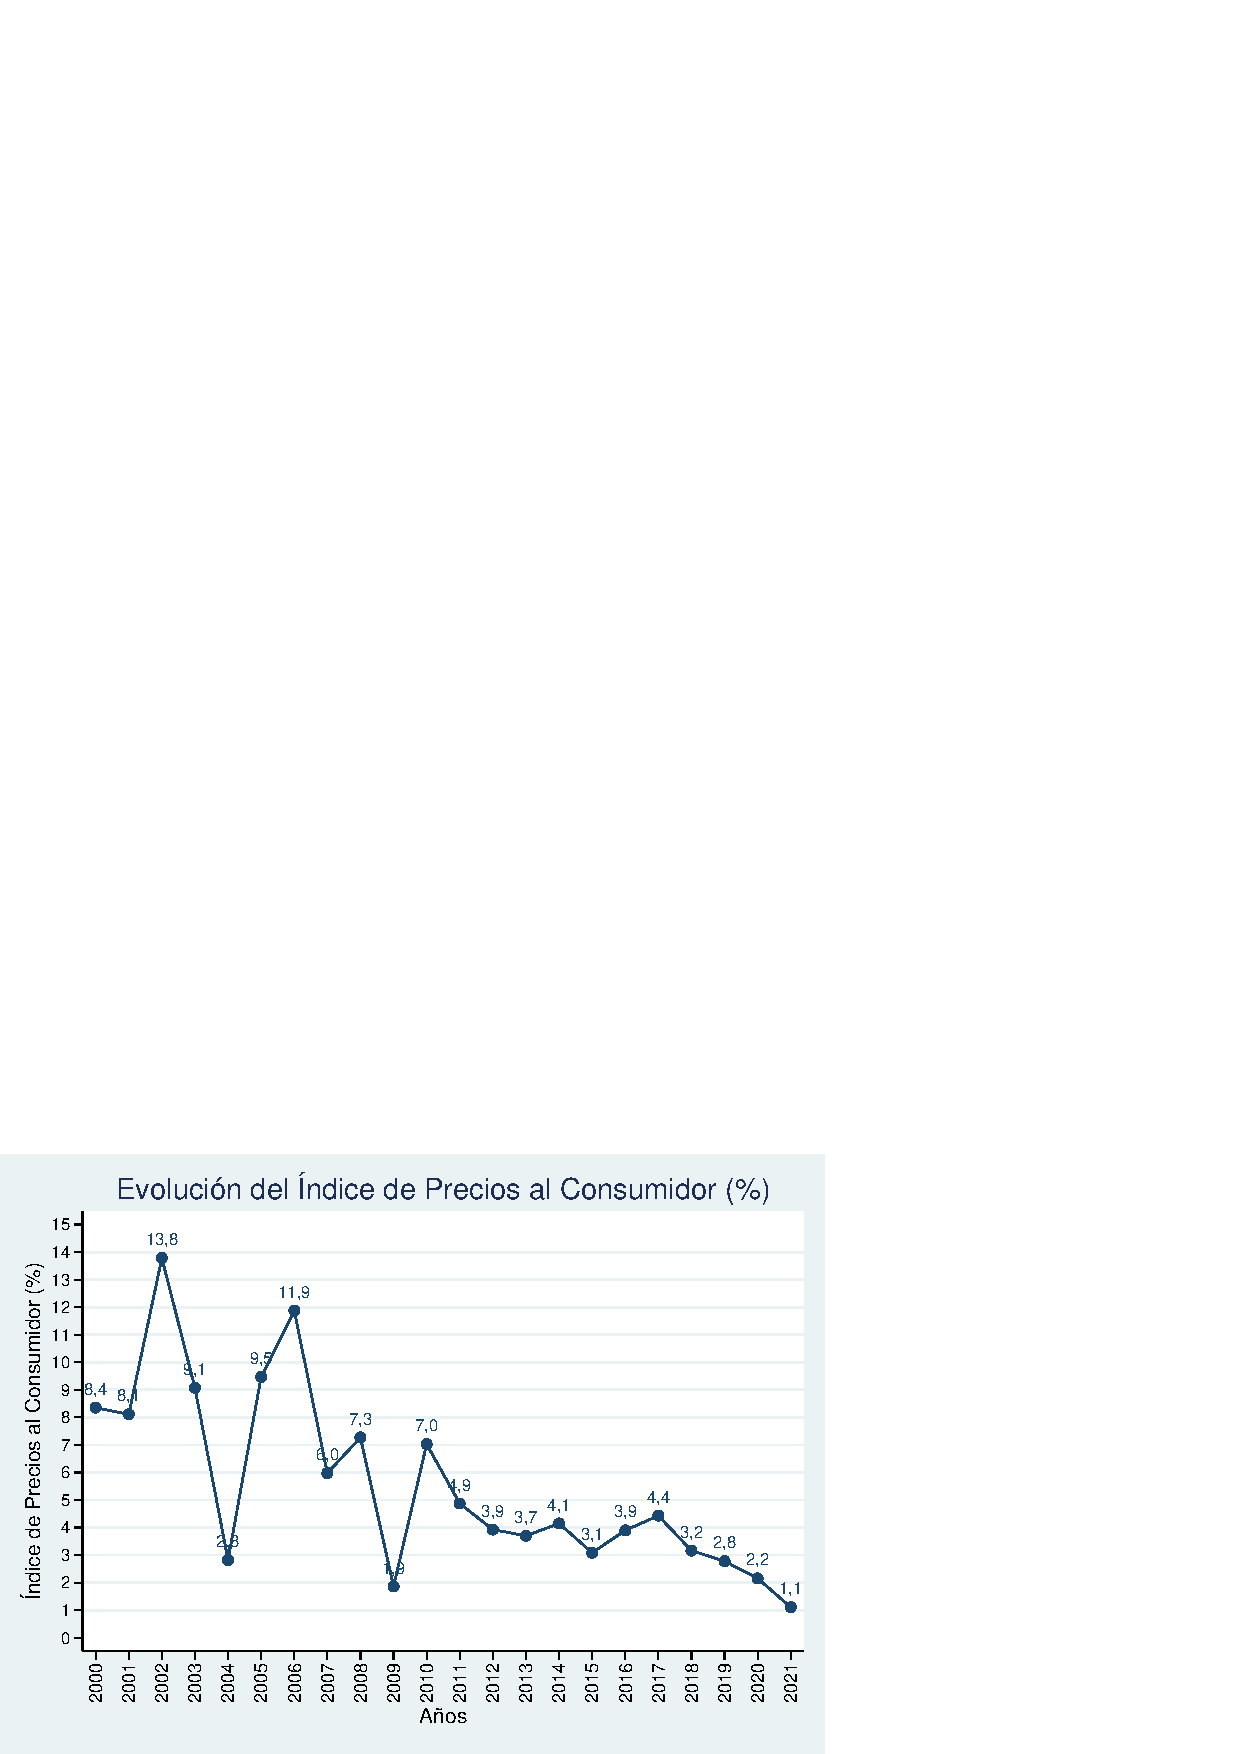
\includegraphics[scale=0.55]{BCP_ipc_year_mes.png}
                                    \item \footnotesize Fuente : Banco Central del Paraguay. 
                                    %\item \footnotesize Nota : 
                    \end{center}
\end{figure}

\subsubsection{Tasa de Interés}

Según el Informe de Estabilidad Financiera del BCP:
\textit{"Durante el año 2020, el impacto económico de la crisis sanitaria asociada a la pandemia ha debilitado a la economía mundial, regional y local".}

En este escenario, el desempeño de las variables macroeconómicas
domésticas fue afectado negativamente por la propagación del COVID-19 y
las medidas de confinamiento implementadas desde finales del primer
trimestre del año 2020 y que, posteriormente fue ron flexibilizadas a
través de una cuarentena inteligente que fue liberando y poniendo en
marcha nuevamente a los sectores económicos.

En el sector financiero, la serie de medidas adoptadas por el BCP para
asegurar la provisión de la liquidez al sistema financiero, mantener el
flujo de crédito y la continuidad de las operaciones de pagos de la
economía, han contribuido con la reactivac ión económica.

Además, en materia de política crediticia se han flexibilizado algunas
reglamentaciones a fin de proporcionar un alivio a la carga financiera
de las empresas y los hogares. Estas medidas han incluido la
reprogramación de créditos, de tal manera a evitar el deterioro de la
clasificación crediticia del cliente, de manera a que pueda seguir
siendo sujeto de crédito, y la facilidad, para las entidades
financieras, de que los cargos generados por las previsiones sean
reconocidos gradualmente en los estados de resultados.

En consecuencia, conforme se esperaba, la cartera renegociada ha
aumentado significativamente. En cuanto a la solvencia, el sistema
financiero no ha enfrentado sobresaltos, considerando que los
indicadores siguen ubicándose, con holgura, por encima de l os
requerimientos mínimos de capital.

Por su parte, la rentabilidad de las entidades ha sido adversamente
afectada, lo que se constata con la disminución del diferencial de tasas
de interés y los ratios ROA(Rentabilidad sobre activos) y ROE (
Rentabilidad sobre patrimonio neto).

La Carta Orgánica del IPS establece que la inversión de los recursos se
debe realizar en las mejores condiciones de seguridad, plazo, garantía y
rendimiento. Adicionalmente establece que los fondos destinados a
inversiones financieras deberán tener un r endimiento similar al de las
tasas pasivas de interés vigentes en el sistema bancario en el momento
de formalizarse la operación, y estarán orientados principalmente a
apoyar el sector productivo.

Al no encontrarse fácilmente tasas referenciales de mercado para un
instrumento financiero contra el cual comparar, ejemplo, un bono emitido
por una entidad financiera de segundo piso, se consideran los demás
elementos (seguridad y garantía), para llega r a conclusiones de sentido
común sobre el peso de estos elementos en cada instrumento de inversión
versus el nivel de tasa (mayor o menor) ofrecida por el mercado a una
fecha determinada y por plazos más o menos similares.

También es importante considerar que las colocaciones que realiza el IPS
en el sistema financiero son principalmente en Certificados de Depósitos
de Ahorro (CDA), lo cual es realizado mediante un sistema competitivo de
ofertas entre todas las institucio nes financieras que cumplan con
ciertos requerimientos de solvencia. Y las tasas aceptadas son por lo
menos iguales al promedio ponderado de tasas publicadas por el BCP del
sistema financiero por plazo y moneda, siendo el promedio de
rentabilidad para d icho instrumento superior a la media de mercado.

\begin{table}[H]
\begin{center}
\caption{\bf{Tasas efectivas de interés. Periodo 2011-2021}}
\begin{tabular}{l|rrrrrr}
\scriptsize
\begin{tabular}{lllllllllllll}
\cline{1-13}
\multicolumn{1}{c}{} &
  \multicolumn{12}{|c}{Mes} \\
\multicolumn{1}{c}{} &
  \multicolumn{1}{|r}{Ene} &
  \multicolumn{1}{r}{Feb} &
  \multicolumn{1}{r}{Mar} &
  \multicolumn{1}{r}{Abr} &
  \multicolumn{1}{r}{May} &
  \multicolumn{1}{r}{Jun} &
  \multicolumn{1}{r}{Jul} &
  \multicolumn{1}{r}{Ago} &
  \multicolumn{1}{r}{Sep} &
  \multicolumn{1}{r}{Oct} &
  \multicolumn{1}{r}{Nov} &
  \multicolumn{1}{r}{Dic} \\
\cline{1-13}
\multicolumn{1}{l}{Año} &
  \multicolumn{1}{|r}{} &
  \multicolumn{1}{r}{} &
  \multicolumn{1}{r}{} &
  \multicolumn{1}{r}{} &
  \multicolumn{1}{r}{} &
  \multicolumn{1}{r}{} &
  \multicolumn{1}{r}{} &
  \multicolumn{1}{r}{} &
  \multicolumn{1}{r}{} &
  \multicolumn{1}{r}{} &
  \multicolumn{1}{r}{} &
  \multicolumn{1}{r}{} \\
\multicolumn{1}{l}{\hspace{1em}2011} &
  \multicolumn{1}{|r}{10,51} &
  \multicolumn{1}{r}{11,18} &
  \multicolumn{1}{r}{11,54} &
  \multicolumn{1}{r}{12,64} &
  \multicolumn{1}{r}{13,38} &
  \multicolumn{1}{r}{13,07} &
  \multicolumn{1}{r}{12,84} &
  \multicolumn{1}{r}{12,00} &
  \multicolumn{1}{r}{12,06} &
  \multicolumn{1}{r}{12,39} &
  \multicolumn{1}{r}{12,48} &
  \multicolumn{1}{r}{12,82} \\
\multicolumn{1}{l}{\hspace{1em}2012} &
  \multicolumn{1}{|r}{12,21} &
  \multicolumn{1}{r}{11,88} &
  \multicolumn{1}{r}{11,78} &
  \multicolumn{1}{r}{12,23} &
  \multicolumn{1}{r}{12,44} &
  \multicolumn{1}{r}{12,57} &
  \multicolumn{1}{r}{12,65} &
  \multicolumn{1}{r}{13,04} &
  \multicolumn{1}{r}{12,63} &
  \multicolumn{1}{r}{12,77} &
  \multicolumn{1}{r}{12,53} &
  \multicolumn{1}{r}{12,10} \\
\multicolumn{1}{l}{\hspace{1em}2013} &
  \multicolumn{1}{|r}{12,52} &
  \multicolumn{1}{r}{12,73} &
  \multicolumn{1}{r}{12,28} &
  \multicolumn{1}{r}{11,42} &
  \multicolumn{1}{r}{11,23} &
  \multicolumn{1}{r}{11,16} &
  \multicolumn{1}{r}{11,27} &
  \multicolumn{1}{r}{11,12} &
  \multicolumn{1}{r}{10,84} &
  \multicolumn{1}{r}{10,91} &
  \multicolumn{1}{r}{11,31} &
  \multicolumn{1}{r}{11,49} \\
\multicolumn{1}{l}{\hspace{1em}2014} &
  \multicolumn{1}{|r}{10,62} &
  \multicolumn{1}{r}{10,60} &
  \multicolumn{1}{r}{11,07} &
  \multicolumn{1}{r}{10,65} &
  \multicolumn{1}{r}{10,45} &
  \multicolumn{1}{r}{10,10} &
  \multicolumn{1}{r}{9,29} &
  \multicolumn{1}{r}{9,10} &
  \multicolumn{1}{r}{8,21} &
  \multicolumn{1}{r}{8,95} &
  \multicolumn{1}{r}{8,74} &
  \multicolumn{1}{r}{8,96} \\
\multicolumn{1}{l}{\hspace{1em}2015} &
  \multicolumn{1}{|r}{8,82} &
  \multicolumn{1}{r}{9,19} &
  \multicolumn{1}{r}{9,07} &
  \multicolumn{1}{r}{8,56} &
  \multicolumn{1}{r}{8,64} &
  \multicolumn{1}{r}{8,66} &
  \multicolumn{1}{r}{8,52} &
  \multicolumn{1}{r}{8,46} &
  \multicolumn{1}{r}{8,84} &
  \multicolumn{1}{r}{8,71} &
  \multicolumn{1}{r}{9,23} &
  \multicolumn{1}{r}{9,63} \\
\multicolumn{1}{l}{\hspace{1em}2016} &
  \multicolumn{1}{|r}{10,15} &
  \multicolumn{1}{r}{10,02} &
  \multicolumn{1}{r}{10,09} &
  \multicolumn{1}{r}{10,45} &
  \multicolumn{1}{r}{10,07} &
  \multicolumn{1}{r}{9,94} &
  \multicolumn{1}{r}{9,66} &
  \multicolumn{1}{r}{9,25} &
  \multicolumn{1}{r}{9,33} &
  \multicolumn{1}{r}{9,20} &
  \multicolumn{1}{r}{9,21} &
  \multicolumn{1}{r}{8,57} \\
\multicolumn{1}{l}{\hspace{1em}2017} &
  \multicolumn{1}{|r}{9,10} &
  \multicolumn{1}{r}{8,73} &
  \multicolumn{1}{r}{8,90} &
  \multicolumn{1}{r}{8,40} &
  \multicolumn{1}{r}{8,57} &
  \multicolumn{1}{r}{8,24} &
  \multicolumn{1}{r}{8,11} &
  \multicolumn{1}{r}{7,62} &
  \multicolumn{1}{r}{7,54} &
  \multicolumn{1}{r}{7,41} &
  \multicolumn{1}{r}{7,58} &
  \multicolumn{1}{r}{7,81} \\
\multicolumn{1}{l}{\hspace{1em}2018} &
  \multicolumn{1}{|r}{7,75} &
  \multicolumn{1}{r}{7,94} &
  \multicolumn{1}{r}{7,86} &
  \multicolumn{1}{r}{7,82} &
  \multicolumn{1}{r}{7,51} &
  \multicolumn{1}{r}{7,64} &
  \multicolumn{1}{r}{7,72} &
  \multicolumn{1}{r}{7,62} &
  \multicolumn{1}{r}{7,67} &
  \multicolumn{1}{r}{8,39} &
  \multicolumn{1}{r}{8,14} &
  \multicolumn{1}{r}{8,58} \\
\multicolumn{1}{l}{\hspace{1em}2019} &
  \multicolumn{1}{|r}{8,26} &
  \multicolumn{1}{r}{8,34} &
  \multicolumn{1}{r}{9,26} &
  \multicolumn{1}{r}{8,33} &
  \multicolumn{1}{r}{8,45} &
  \multicolumn{1}{r}{8,52} &
  \multicolumn{1}{r}{8,10} &
  \multicolumn{1}{r}{8,14} &
  \multicolumn{1}{r}{7,98} &
  \multicolumn{1}{r}{8,08} &
  \multicolumn{1}{r}{7,54} &
  \multicolumn{1}{r}{7,68} \\
\multicolumn{1}{l}{\hspace{1em}2020} &
  \multicolumn{1}{|r}{7,26} &
  \multicolumn{1}{r}{7,09} &
  \multicolumn{1}{r}{7,14} &
  \multicolumn{1}{r}{7,20} &
  \multicolumn{1}{r}{7,16} &
  \multicolumn{1}{r}{7,38} &
  \multicolumn{1}{r}{6,44} &
  \multicolumn{1}{r}{6,58} &
  \multicolumn{1}{r}{6,10} &
  \multicolumn{1}{r}{5,66} &
  \multicolumn{1}{r}{5,87} &
  \multicolumn{1}{r}{5,91} \\
\multicolumn{1}{l}{\hspace{1em}2021} &
  \multicolumn{1}{|r}{6,11} &
  \multicolumn{1}{r}{5,91} &
  \multicolumn{1}{r}{5,91} &
  \multicolumn{1}{r}{6,12} &
  \multicolumn{1}{r}{} &
  \multicolumn{1}{r}{} &
  \multicolumn{1}{r}{} &
  \multicolumn{1}{r}{} &
  \multicolumn{1}{r}{} &
  \multicolumn{1}{r}{} &
  \multicolumn{1}{r}{} &
  \multicolumn{1}{r}{} \\
\cline{1-13}
\end{tabular}

\end{tabular}
                    \item \footnotesize Fuente : Banco Central del Paraguay. 
                    %\item \footnotesize Nota : 
\end{center}
\end{table}

\begin{figure}[H]
\begin{center}
                    \caption{Promedio de tasa de interés anual nominal. Periodo 2017-2020}
                    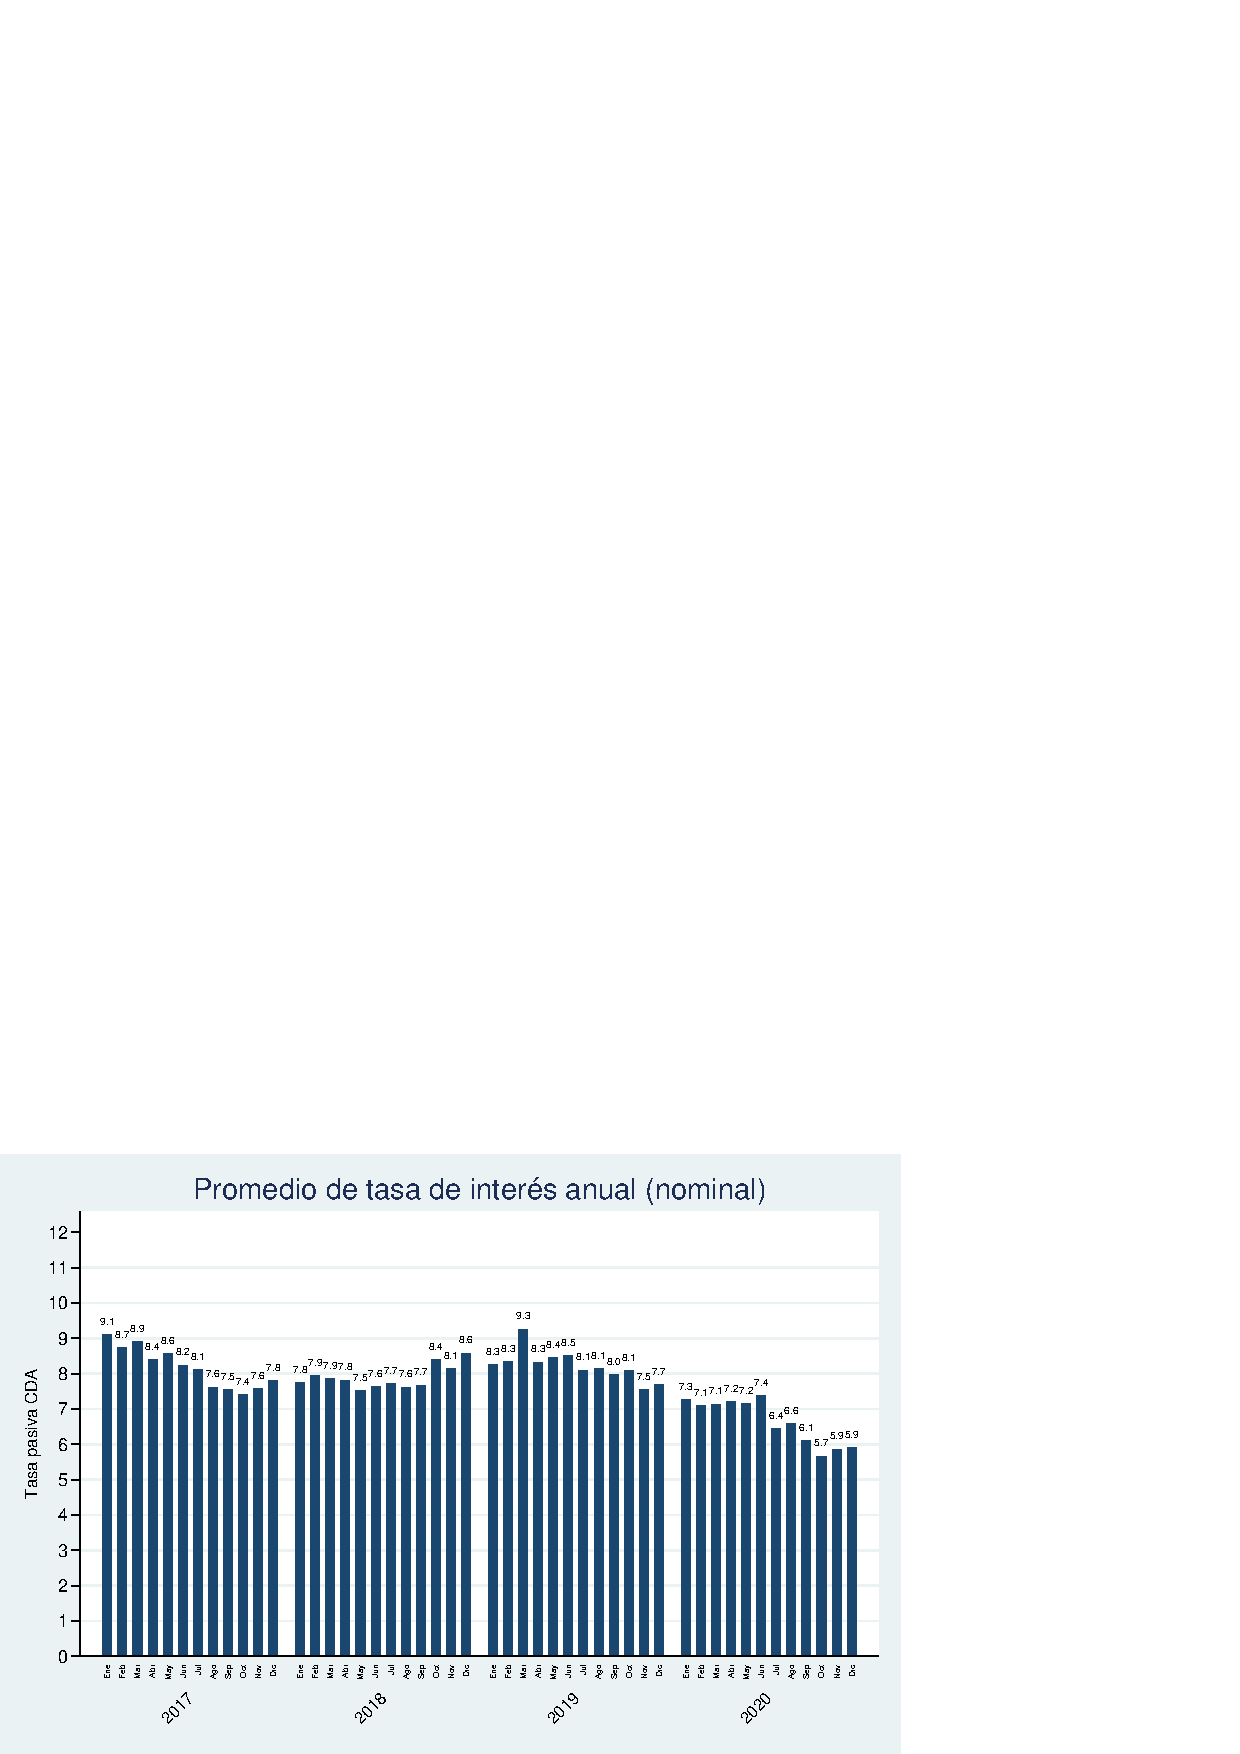
\includegraphics[scale=0.55]{BCP_tasas_pasivas.png}
                                    \item \footnotesize Fuente : Banco Central del Paraguay. 
                                    %\item \footnotesize Nota : 
                    \end{center}
\end{figure}

\subsubsection{Salario Mínimo Legal}

La remuneración mínima o el Salario Mínimo Legal (SML) es la cantidad
mínima de dinero que se le paga a un trabajador en un determinado país y
a través de una Ley establecida oficialmente, para un determinado
período laboral (hora, día o mes), que los e mpleadores deben pagar a
sus trabajadores por sus labores.

Desde el mes de julio del año 2017 se registró un cambio en la
metodología para la determinación del SML con la entrada en vigencia de
la Ley 5764/16 que modifica el Art. 255 del Código del Trabajo, la cual
establece en su artículo 1°:

\textit{"La consideración del salario mínimo será efectuada por el Poder Ejecutivo a propuesta del Consejo Nacional de Salarios Mínimos (CONASAM), sobre la base de la variación interanual del Índice de Precios al Consumidor (IPC) y su impacto en la econ
omía nacional, al mes de junio de cada año". "En los casos de profunda alteración de las condiciones macroeconómicas y financieras o de elevadas tasas de inflación, el Consejo Nacional de Salarios Mínimos podrá reunirse en un periodo distinto al indicad
o anteriormente, y considerará para la fijación del porcentaje del reajuste, los  informes sobre la inflación y la situación económica y financiera del Banco Central del Paraguay y del Ministerio de Hacienda, como así también, las perspectivas o proyecc
iones inflacionarias y económicas respectivas".}

Resulta importante destacar que, con la nueva metodología de ajuste del
Salario Mínimo Legal, lo que se pretende es compensar la pérdida del
poder adquisitivo cada año, no es una suba de salario, sino una
compensación.

Desde el 1 de julio del corriente año entró en vigencia el Decreto N°
5562/21 emitido por el Poder Ejecutivo, en el cual se oficializa el
aumento del salario mínimo en un 4,4\% ascendiendo a Gs. 2.289.324.

Al observar la evolución del SML desde abril de 2005 a junio de 2021, se
aprecia que en los últimos 5 años los niveles de variación se han
mantenido en promedio alrededor del 5\%.

\textbf{****se podría agregar la variación a la Figura 28 y el aumento del SML a Gs. 2.289.324 para el año 2021****}

\begin{figure}[H]
\begin{center}
                    \caption{Evolución del Salario Mínimo Legal. Periodo 2000-2020}
                    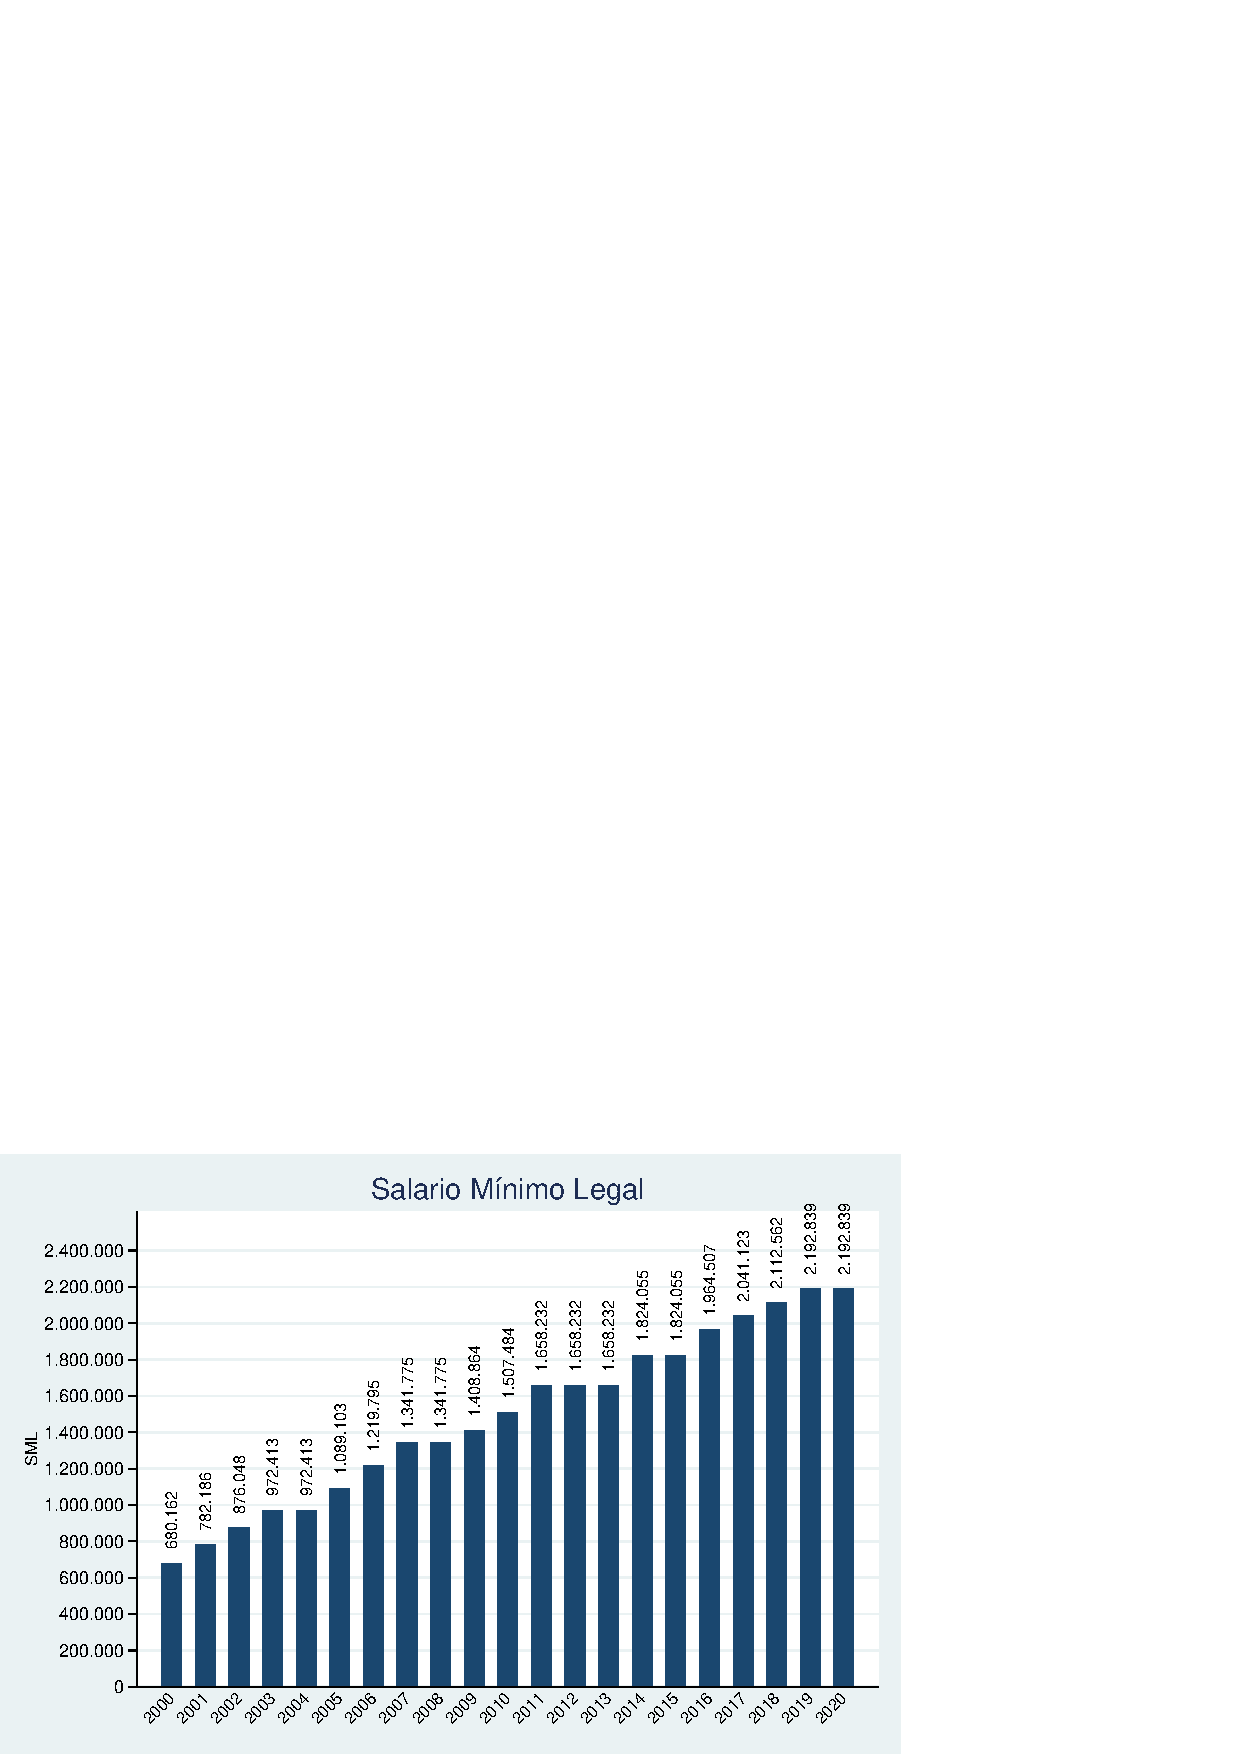
\includegraphics[scale=0.55]{BCP_sml.png}
                                    \item \footnotesize Fuente : Banco Central del Paraguay. 
                                    \item \footnotesize Nota : El SML máximo de enero a diciembre de cada año
                    \end{center}
\end{figure}

\subsubsection{Participación de las remuneraciones en el PIB}

La participación de las remuneraciones en el PIB es un indicador de la
pérdida o ganancia de las remuneraciones laborales en el reparto de la
riqueza generada.

Al observar la evolución de la tasa de participación de las
remuneraciones en el PIB desde el año 2008 al año 2019 se aprecia que si
bien hubo altibajos a lo largo del periodo considerado, la tasa se
estabilizó en torno al 32,5\%.

\begin{table}[H]
\begin{center}
\caption{\bf{Remuneración de asalariados y participación con respecto al PIB. Periodo 2008-2019}}
\begin{tabular}{l|rrrrrr}
\scriptsize
\begin{tabular}{llll}
\cline{1-4}
\multicolumn{1}{c}{} &
  \multicolumn{1}{|r}{Remuneración de asalariados} &
  \multicolumn{1}{r}{PIB (corriente)} &
  \multicolumn{1}{r}{Participación (\%)} \\
\cline{1-4}
\multicolumn{1}{l}{Año} &
  \multicolumn{1}{|r}{} &
  \multicolumn{1}{r}{} &
  \multicolumn{1}{r}{} \\
\multicolumn{1}{l}{\hspace{1em}2008} &
  \multicolumn{1}{|r}{29.448.579,54} &
  \multicolumn{1}{r}{107.403.590,63} &
  \multicolumn{1}{r}{27,42} \\
\multicolumn{1}{l}{\hspace{1em}2009} &
  \multicolumn{1}{|r}{32.625.523,04} &
  \multicolumn{1}{r}{111.030.933,59} &
  \multicolumn{1}{r}{29,38} \\
\multicolumn{1}{l}{\hspace{1em}2010} &
  \multicolumn{1}{|r}{36.976.999,49} &
  \multicolumn{1}{r}{129.092.883,48} &
  \multicolumn{1}{r}{28,64} \\
\multicolumn{1}{l}{\hspace{1em}2011} &
  \multicolumn{1}{|r}{41.443.812,37} &
  \multicolumn{1}{r}{141.486.449,39} &
  \multicolumn{1}{r}{29,29} \\
\multicolumn{1}{l}{\hspace{1em}2012} &
  \multicolumn{1}{|r}{47.214.005,92} &
  \multicolumn{1}{r}{147.225.506,09} &
  \multicolumn{1}{r}{32,07} \\
\multicolumn{1}{l}{\hspace{1em}2013} &
  \multicolumn{1}{|r}{52.209.789,29} &
  \multicolumn{1}{r}{166.350.805,11} &
  \multicolumn{1}{r}{31,39} \\
\multicolumn{1}{l}{\hspace{1em}2014} &
  \multicolumn{1}{|r}{56.662.240,64} &
  \multicolumn{1}{r}{180.174.060,97} &
  \multicolumn{1}{r}{31,45} \\
\multicolumn{1}{l}{\hspace{1em}2015} &
  \multicolumn{1}{|r}{60.164.504,04} &
  \multicolumn{1}{r}{188.477.326,98} &
  \multicolumn{1}{r}{31,92} \\
\multicolumn{1}{l}{\hspace{1em}2016} &
  \multicolumn{1}{|r}{64.338.954,09} &
  \multicolumn{1}{r}{204.647.273,08} &
  \multicolumn{1}{r}{31,44} \\
\multicolumn{1}{l}{\hspace{1em}2017} &
  \multicolumn{1}{|r}{67.329.449,45} &
  \multicolumn{1}{r}{219.122.277,20} &
  \multicolumn{1}{r}{30,73} \\
\multicolumn{1}{l}{\hspace{1em}2018} &
  \multicolumn{1}{|r}{72.961.029,38} &
  \multicolumn{1}{r}{230.576.477,47} &
  \multicolumn{1}{r}{31,64} \\
\multicolumn{1}{l}{\hspace{1em}2019} &
  \multicolumn{1}{|r}{76.770.449,53} &
  \multicolumn{1}{r}{236.566.703,63} &
  \multicolumn{1}{r}{32,45} \\
\cline{1-4}
\end{tabular}

\end{tabular}
                    \item \footnotesize Fuente : Banco Central del Paraguay. 
                    %\item \footnotesize Nota : 
\end{center}
\end{table}

\begin{figure}[H]
\begin{center}
                    \caption{Evolución de las remuneraciones en el PIB. Periodo 2008-2019}
                    \includegraphics[scale=0.55]{BCP_particRemuneraciones.png}
                                    \item \footnotesize Fuente : Banco Central del Paraguay.        %\item \footnotesize Nota : 
                    \end{center}
\end{figure}

\newpage
\newpage

\subsection{Principales datos socio-demográficos del IPS}

\subsubsection{Indicadores anuales de los trabajadores activos cotizantes al fondo de jubilaciones (personas)}

Cabe mencionar que es necesario asumir una definición concreta del
trabajador activo para generar las estadísticas. Para los fines
específicos del Informe Actuarial se considera como trabajador activo
cotizante al Fondo de Jubilaciones y Pensiones en un año determinado, a
todo trabajador que figure en la base de datos. Las bases de datos (BD)
de la DAOP son dinámicas, en el sentido que las cantidades pueden ir
modificándose a medida que se actualizan o adicionan datos que
generalmente corresponden a p agos (aportes) que se realizan con cierta
demora o atrasos. En este caso particular, la BD utilizada fue generada
en fecha 22/05/2018. Las cifras pueden presentar diferencias con las
publicadas por la DIPLAN en sus anuarios debido a la fecha de corte pa
ra la obtención de estas o bien debido a las distintas definiciones
utilizadas para generar las estadísticas.
\footnote{Las bases de datos (BD) de la DAOP son dinámicas, en el sentido que las cantidades pueden ir modificándose a medida que se actualizan
 o adicionan datos que generalmente corresponden a pagos (aportes) que se realizan con cierta demora o atrasos. En este caso particular, la BD utilizada fue generada en fecha 22/05/2018. Las cifras pueden presentar diferencias con las publicadas por la 
DIPLAN en sus anuarios debido a la fecha de corte para la obtención de estas o bien debido a las distintas definiciones utilizadas para generar las estadísticas.}
con al menos un aporte registrado en dicho año. Las cantidades de
activos y los salarios c orresponden a la planilla de pagos del mes de
enero a diciembre del año 2020, de acuerdo al mes en el cual se haya
registrado el último
aporte\footnote{Del total de cotizantes registrados a la fecha de consulta de la base},
se registraron 580.524 cotiza ntes en el mes de enero, para diciembre
presentaron cotización 547.571 personas, marcando así una disminución de
cotizantes al termino del año en un 5.68\% . Para dicho año, el IPS
contaba con 712.309 activos cotizantes del Fondo de J y P de 15 y más
años de edad, de los cuales 258.003 (36,22\%) eran mujeres y 454.306
hombres (63,78\%). El grupo más numeroso se encontraba en la franja
etaria comprendida entre los 20 y 41 años.

\textbf{Características de los cotizantes en el año 2020}

\begin{table}[H]
\begin{center}
\scriptsize
\caption{\bf{Cantidad de cotizantes por edades, según año (Personas)}}
\begin{tabular}{l|rrrrrrrrrrrrr}
\textbf{edadtop} & \multicolumn{2}{c}{\textbf{Hombres}} & \multicolumn{2}{c}{\textbf{Mujeres}} & \multicolumn{2}{c}{\textbf{Total}} \\
&Cant.&Porc.&Cant.&Porc.&Cant.&Porc. \\
\hline
18 y menos&4.353&0,96\%&1.737&0,67\%&6.090&0,85\% \\
19&8.247&1,82\%&3.751&1,45\%&11.998&1,68\% \\
20&11.318&2,49\%&6.069&2,35\%&17.387&2,44\% \\
21&13.836&3,05\%&7.728&3,00\%&21.564&3,03\% \\
22&15.253&3,36\%&9.140&3,54\%&24.393&3,42\% \\
23&17.075&3,76\%&10.295&3,99\%&27.370&3,84\% \\
24&17.865&3,93\%&11.424&4,43\%&29.289&4,11\% \\
25&17.935&3,95\%&11.428&4,43\%&29.363&4,12\% \\
26&18.150&4,00\%&11.646&4,51\%&29.796&4,18\% \\
27&18.170&4,00\%&11.782&4,57\%&29.952&4,20\% \\
28&18.243&4,02\%&11.576&4,49\%&29.819&4,19\% \\
29&17.993&3,96\%&11.460&4,44\%&29.453&4,13\% \\
30&17.176&3,78\%&10.636&4,12\%&27.812&3,90\% \\
31&16.613&3,66\%&10.049&3,89\%&26.662&3,74\% \\
32&15.591&3,43\%&9.352&3,62\%&24.943&3,50\% \\
33&14.744&3,25\%&8.608&3,34\%&23.352&3,28\% \\
34&14.162&3,12\%&8.354&3,24\%&22.516&3,16\% \\
35&13.733&3,02\%&7.785&3,02\%&21.518&3,02\% \\
36&13.754&3,03\%&7.680&2,98\%&21.434&3,01\% \\
37&13.091&2,88\%&7.147&2,77\%&20.238&2,84\% \\
38&12.610&2,78\%&7.060&2,74\%&19.670&2,76\% \\
39&11.306&2,49\%&6.224&2,41\%&17.530&2,46\% \\
40&10.909&2,40\%&5.942&2,30\%&16.851&2,37\% \\
41&9.760&2,15\%&5.028&1,95\%&14.788&2,08\% \\
42&8.501&1,87\%&4.632&1,80\%&13.133&1,84\% \\
43&7.973&1,75\%&4.080&1,58\%&12.053&1,69\% \\
44&7.322&1,61\%&3.789&1,47\%&11.111&1,56\% \\
45&6.834&1,50\%&3.489&1,35\%&10.323&1,45\% \\
46&6.382&1,40\%&3.282&1,27\%&9.664&1,36\% \\
47&5.942&1,31\%&2.976&1,15\%&8.918&1,25\% \\
48&5.893&1,30\%&2.906&1,13\%&8.799&1,24\% \\
49&5.530&1,22\%&2.791&1,08\%&8.321&1,17\% \\
50&5.404&1,19\%&2.621&1,02\%&8.025&1,13\% \\
51&5.062&1,11\%&2.431&0,94\%&7.493&1,05\% \\
52&4.817&1,06\%&2.407&0,93\%&7.224&1,01\% \\
53&4.360&0,96\%&2.121&0,82\%&6.481&0,91\% \\
54&4.400&0,97\%&2.085&0,81\%&6.485&0,91\% \\
55&4.158&0,92\%&2.006&0,78\%&6.164&0,87\% \\
56&3.762&0,83\%&1.828&0,71\%&5.590&0,78\% \\
57&3.593&0,79\%&1.700&0,66\%&5.293&0,74\% \\
58&3.200&0,70\%&1.516&0,59\%&4.716&0,66\% \\
59&3.342&0,74\%&1.667&0,65\%&5.009&0,70\% \\
60&2.676&0,59\%&1.266&0,49\%&3.942&0,55\% \\
61&2.078&0,46\%&986&0,38\%&3.064&0,43\% \\
62&1.814&0,40\%&841&0,33\%&2.655&0,37\% \\
63&1.686&0,37\%&748&0,29\%&2.434&0,34\% \\
64&1.662&0,37\%&705&0,27\%&2.367&0,33\% \\
65&1.270&0,28\%&541&0,21\%&1.811&0,25\% \\
66&849&0,19\%&504&0,20\%&1.353&0,19\% \\
67&726&0,16\%&373&0,14\%&1.099&0,15\% \\
68&604&0,13\%&288&0,11\%&892&0,13\% \\
69&477&0,10\%&226&0,09\%&703&0,10\% \\
70 y más&2.102&0,46\%&1.297&0,50\%&3.399&0,48\% \\
\textbf{Total}&454.306&100,00\%&258.003&100,00\%&712.309&100,00\% \\

\end{tabular}
                            \item Fuente : Elaboración própia a partir de registros administrativos del IPS.
\end{center}
\end{table}

\begin{figure}[H]
\begin{center}
                    \caption{Distribución de la cantidad de personas cotizantes al FJ por edad y sexo}
                    \vspace{0.5cm}
                    \includegraphics[scale=0.4]{RA_IPS_cotizantes_2020_sexo_edad_18a70.png}
\end{center}
\end{figure}

\begin{table}[H]
\begin{center}
\scriptsize
\caption{\bf{Distribución de la cantidad de personas cotizantes al FJ por tramos de edad y sexo}}
\begin{tabular}{l|rrrrrrrrrrrrr}
\input{RA_IPS_cotizantes_2020_sexo_edadt_18a70}
\end{tabular}
                    \item Fuente : Elaboración própia a partir de registros administrativos del IPS.
\end{center}
\end{table}

\begin{figure}[H]
\begin{center}
                    \caption{Pirámide de población - (Cotizantes. Año 2020)}
                    \vspace{0.5cm}
                    \includegraphics[scale=0.6]{RA_IPS_cotizantes_2020_sexo_edadt_piramide.png}
\end{center}
\end{figure}

\begin{table}[H]
\begin{center}
\scriptsize
\caption{\bf{Salario promedio de las personas cotizantes al FJ por edad y sexo}}
\begin{tabular}{l|rrrrrrrrrrrrr}
\begin{tabular}{llll}
\cline{1-4}
\multicolumn{1}{c}{} &
  \multicolumn{3}{|c}{Sexo} \\
\multicolumn{1}{c}{} &
  \multicolumn{1}{|r}{Hombres} &
  \multicolumn{1}{r}{Mujeres} &
  \multicolumn{1}{r}{Total} \\
\cline{1-4}
\multicolumn{1}{l}{Edad} &
  \multicolumn{1}{|r}{} &
  \multicolumn{1}{r}{} &
  \multicolumn{1}{r}{} \\
\multicolumn{1}{l}{\hspace{1em}18 y menos} &
  \multicolumn{1}{|r}{1.647.398} &
  \multicolumn{1}{r}{1.573.401} &
  \multicolumn{1}{r}{1.647.398} \\
\multicolumn{1}{l}{\hspace{1em}19} &
  \multicolumn{1}{|r}{1.869.872} &
  \multicolumn{1}{r}{1.831.838} &
  \multicolumn{1}{r}{1.869.872} \\
\multicolumn{1}{l}{\hspace{1em}20} &
  \multicolumn{1}{|r}{2.057.655} &
  \multicolumn{1}{r}{2.044.521} &
  \multicolumn{1}{r}{2.057.655} \\
\multicolumn{1}{l}{\hspace{1em}21} &
  \multicolumn{1}{|r}{2.199.210} &
  \multicolumn{1}{r}{2.161.953} &
  \multicolumn{1}{r}{2.199.210} \\
\multicolumn{1}{l}{\hspace{1em}22} &
  \multicolumn{1}{|r}{2.295.259} &
  \multicolumn{1}{r}{2.251.440} &
  \multicolumn{1}{r}{2.295.259} \\
\multicolumn{1}{l}{\hspace{1em}23} &
  \multicolumn{1}{|r}{2.415.027} &
  \multicolumn{1}{r}{2.386.680} &
  \multicolumn{1}{r}{2.415.027} \\
\multicolumn{1}{l}{\hspace{1em}24} &
  \multicolumn{1}{|r}{2.539.971} &
  \multicolumn{1}{r}{2.520.227} &
  \multicolumn{1}{r}{2.539.971} \\
\multicolumn{1}{l}{\hspace{1em}25} &
  \multicolumn{1}{|r}{2.675.760} &
  \multicolumn{1}{r}{2.681.596} &
  \multicolumn{1}{r}{2.681.596} \\
\multicolumn{1}{l}{\hspace{1em}26} &
  \multicolumn{1}{|r}{2.868.071} &
  \multicolumn{1}{r}{2.836.183} &
  \multicolumn{1}{r}{2.868.071} \\
\multicolumn{1}{l}{\hspace{1em}27} &
  \multicolumn{1}{|r}{2.972.912} &
  \multicolumn{1}{r}{3.000.978} &
  \multicolumn{1}{r}{3.000.978} \\
\multicolumn{1}{l}{\hspace{1em}28} &
  \multicolumn{1}{|r}{3.095.174} &
  \multicolumn{1}{r}{3.084.374} &
  \multicolumn{1}{r}{3.095.174} \\
\multicolumn{1}{l}{\hspace{1em}29} &
  \multicolumn{1}{|r}{3.252.230} &
  \multicolumn{1}{r}{3.200.132} &
  \multicolumn{1}{r}{3.252.230} \\
\multicolumn{1}{l}{\hspace{1em}30} &
  \multicolumn{1}{|r}{3.384.950} &
  \multicolumn{1}{r}{3.335.319} &
  \multicolumn{1}{r}{3.384.950} \\
\multicolumn{1}{l}{\hspace{1em}31} &
  \multicolumn{1}{|r}{3.554.837} &
  \multicolumn{1}{r}{3.446.023} &
  \multicolumn{1}{r}{3.554.837} \\
\multicolumn{1}{l}{\hspace{1em}32} &
  \multicolumn{1}{|r}{3.643.920} &
  \multicolumn{1}{r}{3.641.841} &
  \multicolumn{1}{r}{3.643.920} \\
\multicolumn{1}{l}{\hspace{1em}33} &
  \multicolumn{1}{|r}{3.705.939} &
  \multicolumn{1}{r}{3.671.003} &
  \multicolumn{1}{r}{3.705.939} \\
\multicolumn{1}{l}{\hspace{1em}34} &
  \multicolumn{1}{|r}{3.888.751} &
  \multicolumn{1}{r}{3.738.498} &
  \multicolumn{1}{r}{3.888.751} \\
\multicolumn{1}{l}{\hspace{1em}35} &
  \multicolumn{1}{|r}{3.965.026} &
  \multicolumn{1}{r}{3.825.647} &
  \multicolumn{1}{r}{3.965.026} \\
\multicolumn{1}{l}{\hspace{1em}36} &
  \multicolumn{1}{|r}{3.996.414} &
  \multicolumn{1}{r}{3.900.499} &
  \multicolumn{1}{r}{3.996.414} \\
\multicolumn{1}{l}{\hspace{1em}37} &
  \multicolumn{1}{|r}{4.055.798} &
  \multicolumn{1}{r}{3.892.665} &
  \multicolumn{1}{r}{4.055.798} \\
\multicolumn{1}{l}{\hspace{1em}38} &
  \multicolumn{1}{|r}{4.154.389} &
  \multicolumn{1}{r}{3.949.822} &
  \multicolumn{1}{r}{4.154.389} \\
\multicolumn{1}{l}{\hspace{1em}39} &
  \multicolumn{1}{|r}{4.210.606} &
  \multicolumn{1}{r}{3.994.473} &
  \multicolumn{1}{r}{4.210.606} \\
\multicolumn{1}{l}{\hspace{1em}40} &
  \multicolumn{1}{|r}{4.179.287} &
  \multicolumn{1}{r}{4.003.800} &
  \multicolumn{1}{r}{4.179.287} \\
\multicolumn{1}{l}{\hspace{1em}41} &
  \multicolumn{1}{|r}{4.145.900} &
  \multicolumn{1}{r}{3.912.505} &
  \multicolumn{1}{r}{4.145.900} \\
\multicolumn{1}{l}{\hspace{1em}42} &
  \multicolumn{1}{|r}{4.335.325} &
  \multicolumn{1}{r}{3.977.352} &
  \multicolumn{1}{r}{4.335.325} \\
\multicolumn{1}{l}{\hspace{1em}43} &
  \multicolumn{1}{|r}{4.218.473} &
  \multicolumn{1}{r}{3.853.365} &
  \multicolumn{1}{r}{4.218.473} \\
\multicolumn{1}{l}{\hspace{1em}44} &
  \multicolumn{1}{|r}{4.390.030} &
  \multicolumn{1}{r}{3.978.599} &
  \multicolumn{1}{r}{4.390.030} \\
\multicolumn{1}{l}{\hspace{1em}45} &
  \multicolumn{1}{|r}{4.173.082} &
  \multicolumn{1}{r}{3.955.129} &
  \multicolumn{1}{r}{4.173.082} \\
\multicolumn{1}{l}{\hspace{1em}46} &
  \multicolumn{1}{|r}{4.199.792} &
  \multicolumn{1}{r}{3.830.997} &
  \multicolumn{1}{r}{4.199.792} \\
\multicolumn{1}{l}{\hspace{1em}47} &
  \multicolumn{1}{|r}{4.223.070} &
  \multicolumn{1}{r}{3.895.532} &
  \multicolumn{1}{r}{4.223.070} \\
\multicolumn{1}{l}{\hspace{1em}48} &
  \multicolumn{1}{|r}{4.150.393} &
  \multicolumn{1}{r}{3.854.828} &
  \multicolumn{1}{r}{4.150.393} \\
\multicolumn{1}{l}{\hspace{1em}49} &
  \multicolumn{1}{|r}{4.307.933} &
  \multicolumn{1}{r}{3.711.392} &
  \multicolumn{1}{r}{4.307.933} \\
\multicolumn{1}{l}{\hspace{1em}50} &
  \multicolumn{1}{|r}{4.290.013} &
  \multicolumn{1}{r}{3.643.976} &
  \multicolumn{1}{r}{4.290.013} \\
\multicolumn{1}{l}{\hspace{1em}51} &
  \multicolumn{1}{|r}{4.374.196} &
  \multicolumn{1}{r}{3.682.849} &
  \multicolumn{1}{r}{4.374.196} \\
\multicolumn{1}{l}{\hspace{1em}52} &
  \multicolumn{1}{|r}{4.273.379} &
  \multicolumn{1}{r}{3.796.620} &
  \multicolumn{1}{r}{4.273.379} \\
\multicolumn{1}{l}{\hspace{1em}53} &
  \multicolumn{1}{|r}{4.447.214} &
  \multicolumn{1}{r}{3.746.920} &
  \multicolumn{1}{r}{4.447.214} \\
\multicolumn{1}{l}{\hspace{1em}54} &
  \multicolumn{1}{|r}{4.383.349} &
  \multicolumn{1}{r}{3.732.247} &
  \multicolumn{1}{r}{4.383.349} \\
\multicolumn{1}{l}{\hspace{1em}55} &
  \multicolumn{1}{|r}{4.339.178} &
  \multicolumn{1}{r}{3.696.614} &
  \multicolumn{1}{r}{4.339.178} \\
\multicolumn{1}{l}{\hspace{1em}56} &
  \multicolumn{1}{|r}{4.114.072} &
  \multicolumn{1}{r}{3.637.128} &
  \multicolumn{1}{r}{4.114.072} \\
\multicolumn{1}{l}{\hspace{1em}57} &
  \multicolumn{1}{|r}{4.440.151} &
  \multicolumn{1}{r}{3.367.925} &
  \multicolumn{1}{r}{4.440.151} \\
\multicolumn{1}{l}{\hspace{1em}58} &
  \multicolumn{1}{|r}{4.418.159} &
  \multicolumn{1}{r}{3.406.333} &
  \multicolumn{1}{r}{4.418.159} \\
\multicolumn{1}{l}{\hspace{1em}59} &
  \multicolumn{1}{|r}{5.165.371} &
  \multicolumn{1}{r}{3.620.060} &
  \multicolumn{1}{r}{5.165.371} \\
\multicolumn{1}{l}{\hspace{1em}60} &
  \multicolumn{1}{|r}{3.808.506} &
  \multicolumn{1}{r}{2.984.610} &
  \multicolumn{1}{r}{3.808.506} \\
\multicolumn{1}{l}{\hspace{1em}61} &
  \multicolumn{1}{|r}{3.607.189} &
  \multicolumn{1}{r}{3.164.331} &
  \multicolumn{1}{r}{3.607.189} \\
\multicolumn{1}{l}{\hspace{1em}62} &
  \multicolumn{1}{|r}{3.499.128} &
  \multicolumn{1}{r}{3.037.496} &
  \multicolumn{1}{r}{3.499.128} \\
\multicolumn{1}{l}{\hspace{1em}63} &
  \multicolumn{1}{|r}{3.554.975} &
  \multicolumn{1}{r}{2.848.443} &
  \multicolumn{1}{r}{3.554.975} \\
\multicolumn{1}{l}{\hspace{1em}64} &
  \multicolumn{1}{|r}{3.548.208} &
  \multicolumn{1}{r}{3.072.533} &
  \multicolumn{1}{r}{3.548.208} \\
\multicolumn{1}{l}{\hspace{1em}65} &
  \multicolumn{1}{|r}{3.506.993} &
  \multicolumn{1}{r}{3.207.342} &
  \multicolumn{1}{r}{3.506.993} \\
\multicolumn{1}{l}{\hspace{1em}66} &
  \multicolumn{1}{|r}{3.307.243} &
  \multicolumn{1}{r}{3.093.894} &
  \multicolumn{1}{r}{3.307.243} \\
\multicolumn{1}{l}{\hspace{1em}67} &
  \multicolumn{1}{|r}{3.617.030} &
  \multicolumn{1}{r}{2.502.379} &
  \multicolumn{1}{r}{3.617.030} \\
\multicolumn{1}{l}{\hspace{1em}68} &
  \multicolumn{1}{|r}{3.312.891} &
  \multicolumn{1}{r}{2.415.898} &
  \multicolumn{1}{r}{3.312.891} \\
\multicolumn{1}{l}{\hspace{1em}69} &
  \multicolumn{1}{|r}{3.391.157} &
  \multicolumn{1}{r}{3.035.660} &
  \multicolumn{1}{r}{3.391.157} \\
\multicolumn{1}{l}{\hspace{1em}70 y más} &
  \multicolumn{1}{|r}{2.897.203} &
  \multicolumn{1}{r}{2.308.935} &
  \multicolumn{1}{r}{2.897.203} \\
\multicolumn{1}{l}{\hspace{1em}Total} &
  \multicolumn{1}{|r}{5.165.371} &
  \multicolumn{1}{r}{4.003.800} &
  \multicolumn{1}{r}{5.165.371} \\
\cline{1-4}
\end{tabular}

\end{tabular}
                    \item Fuente : Elaboración própia a partir de registros administrativos del IPS.
\end{center}
\end{table}

\begin{figure}[H]
\begin{center}
                    \caption{Salario promedio de las personas cotizantes al FJ por edad y sexo"}
                    \vspace{0.5cm}
                    \includegraphics[scale=0.6]{RA_IPS_cotizantes_2020_sexo_edad_18a70_salprom.png}
\end{center}
\end{figure}

\begin{table}[H]
\begin{center}
\scriptsize
\caption{\bf{Distribución de salarios por percentiles. (Año 2020 - Hombres)}}
\begin{tabular}{l|rrrrrrrrrrrrr}
\begin{tabular}{llllllllll}
\cline{1-10}
\multicolumn{1}{c}{} &
  \multicolumn{1}{|r}{P10} &
  \multicolumn{1}{r}{P20} &
  \multicolumn{1}{r}{P30} &
  \multicolumn{1}{r}{P40} &
  \multicolumn{1}{r}{P50} &
  \multicolumn{1}{r}{P60} &
  \multicolumn{1}{r}{P70} &
  \multicolumn{1}{r}{P80} &
  \multicolumn{1}{r}{P90} \\
\cline{1-10}
\multicolumn{1}{l}{Edad} &
  \multicolumn{1}{|r}{} &
  \multicolumn{1}{r}{} &
  \multicolumn{1}{r}{} &
  \multicolumn{1}{r}{} &
  \multicolumn{1}{r}{} &
  \multicolumn{1}{r}{} &
  \multicolumn{1}{r}{} &
  \multicolumn{1}{r}{} &
  \multicolumn{1}{r}{} \\
\multicolumn{1}{l}{\hspace{1em}18 y menos} &
  \multicolumn{1}{|r}{337.385} &
  \multicolumn{1}{r}{708.456} &
  \multicolumn{1}{r}{1.040.000} &
  \multicolumn{1}{r}{1.461.892} &
  \multicolumn{1}{r}{1.579.969} &
  \multicolumn{1}{r}{2.074.060} &
  \multicolumn{1}{r}{2.192.839} &
  \multicolumn{1}{r}{2.240.662} &
  \multicolumn{1}{r}{2.625.671} \\
\multicolumn{1}{l}{\hspace{1em}19} &
  \multicolumn{1}{|r}{455.435} &
  \multicolumn{1}{r}{910.871} &
  \multicolumn{1}{r}{1.330.333} &
  \multicolumn{1}{r}{1.518.120} &
  \multicolumn{1}{r}{2.046.649} &
  \multicolumn{1}{r}{2.192.839} &
  \multicolumn{1}{r}{2.192.839} &
  \multicolumn{1}{r}{2.381.064} &
  \multicolumn{1}{r}{2.885.690} \\
\multicolumn{1}{l}{\hspace{1em}20} &
  \multicolumn{1}{|r}{556.644} &
  \multicolumn{1}{r}{1.096.420} &
  \multicolumn{1}{r}{1.518.120} &
  \multicolumn{1}{r}{1.906.667} &
  \multicolumn{1}{r}{2.192.839} &
  \multicolumn{1}{r}{2.192.839} &
  \multicolumn{1}{r}{2.265.934} &
  \multicolumn{1}{r}{2.517.663} &
  \multicolumn{1}{r}{3.152.058} \\
\multicolumn{1}{l}{\hspace{1em}21} &
  \multicolumn{1}{|r}{631.868} &
  \multicolumn{1}{r}{1.254.428} &
  \multicolumn{1}{r}{1.518.120} &
  \multicolumn{1}{r}{2.108.500} &
  \multicolumn{1}{r}{2.192.839} &
  \multicolumn{1}{r}{2.192.839} &
  \multicolumn{1}{r}{2.339.028} &
  \multicolumn{1}{r}{2.644.812} &
  \multicolumn{1}{r}{3.359.527} \\
\multicolumn{1}{l}{\hspace{1em}22} &
  \multicolumn{1}{|r}{674.720} &
  \multicolumn{1}{r}{1.315.704} &
  \multicolumn{1}{r}{1.648.352} &
  \multicolumn{1}{r}{2.192.839} &
  \multicolumn{1}{r}{2.192.839} &
  \multicolumn{1}{r}{2.193.000} &
  \multicolumn{1}{r}{2.434.051} &
  \multicolumn{1}{r}{2.792.839} &
  \multicolumn{1}{r}{3.555.125} \\
\multicolumn{1}{l}{\hspace{1em}23} &
  \multicolumn{1}{|r}{730.946} &
  \multicolumn{1}{r}{1.461.892} &
  \multicolumn{1}{r}{1.827.365} &
  \multicolumn{1}{r}{2.192.839} &
  \multicolumn{1}{r}{2.192.839} &
  \multicolumn{1}{r}{2.256.994} &
  \multicolumn{1}{r}{2.500.000} &
  \multicolumn{1}{r}{2.918.375} &
  \multicolumn{1}{r}{3.795.300} \\
\multicolumn{1}{l}{\hspace{1em}24} &
  \multicolumn{1}{|r}{804.041} &
  \multicolumn{1}{r}{1.518.120} &
  \multicolumn{1}{r}{2.005.600} &
  \multicolumn{1}{r}{2.192.839} &
  \multicolumn{1}{r}{2.192.839} &
  \multicolumn{1}{r}{2.311.331} &
  \multicolumn{1}{r}{2.603.996} &
  \multicolumn{1}{r}{3.084.499} &
  \multicolumn{1}{r}{4.084.563} \\
\multicolumn{1}{l}{\hspace{1em}25} &
  \multicolumn{1}{|r}{840.000} &
  \multicolumn{1}{r}{1.518.120} &
  \multicolumn{1}{r}{2.092.842} &
  \multicolumn{1}{r}{2.192.839} &
  \multicolumn{1}{r}{2.192.839} &
  \multicolumn{1}{r}{2.407.063} &
  \multicolumn{1}{r}{2.750.000} &
  \multicolumn{1}{r}{3.296.703} &
  \multicolumn{1}{r}{4.467.255} \\
\multicolumn{1}{l}{\hspace{1em}26} &
  \multicolumn{1}{|r}{910.871} &
  \multicolumn{1}{r}{1.518.120} &
  \multicolumn{1}{r}{2.185.390} &
  \multicolumn{1}{r}{2.192.839} &
  \multicolumn{1}{r}{2.193.000} &
  \multicolumn{1}{r}{2.500.000} &
  \multicolumn{1}{r}{2.888.256} &
  \multicolumn{1}{r}{3.500.000} &
  \multicolumn{1}{r}{4.874.011} \\
\multicolumn{1}{l}{\hspace{1em}27} &
  \multicolumn{1}{|r}{935.077} &
  \multicolumn{1}{r}{1.518.120} &
  \multicolumn{1}{r}{2.192.839} &
  \multicolumn{1}{r}{2.192.839} &
  \multicolumn{1}{r}{2.198.611} &
  \multicolumn{1}{r}{2.500.000} &
  \multicolumn{1}{r}{2.991.673} &
  \multicolumn{1}{r}{3.615.389} &
  \multicolumn{1}{r}{5.016.348} \\
\multicolumn{1}{l}{\hspace{1em}28} &
  \multicolumn{1}{|r}{935.077} &
  \multicolumn{1}{r}{1.518.120} &
  \multicolumn{1}{r}{2.192.839} &
  \multicolumn{1}{r}{2.192.839} &
  \multicolumn{1}{r}{2.260.000} &
  \multicolumn{1}{r}{2.600.000} &
  \multicolumn{1}{r}{3.025.989} &
  \multicolumn{1}{r}{3.782.839} &
  \multicolumn{1}{r}{5.438.039} \\
\multicolumn{1}{l}{\hspace{1em}29} &
  \multicolumn{1}{|r}{935.077} &
  \multicolumn{1}{r}{1.518.120} &
  \multicolumn{1}{r}{2.192.839} &
  \multicolumn{1}{r}{2.192.839} &
  \multicolumn{1}{r}{2.265.934} &
  \multicolumn{1}{r}{2.650.051} &
  \multicolumn{1}{r}{3.145.164} &
  \multicolumn{1}{r}{4.000.000} &
  \multicolumn{1}{r}{5.701.382} \\
\multicolumn{1}{l}{\hspace{1em}30} &
  \multicolumn{1}{|r}{935.077} &
  \multicolumn{1}{r}{1.518.120} &
  \multicolumn{1}{r}{2.192.839} &
  \multicolumn{1}{r}{2.192.839} &
  \multicolumn{1}{r}{2.307.702} &
  \multicolumn{1}{r}{2.731.431} &
  \multicolumn{1}{r}{3.261.810} &
  \multicolumn{1}{r}{4.110.643} &
  \multicolumn{1}{r}{6.209.554} \\
\multicolumn{1}{l}{\hspace{1em}31} &
  \multicolumn{1}{|r}{961.476} &
  \multicolumn{1}{r}{1.518.120} &
  \multicolumn{1}{r}{2.192.839} &
  \multicolumn{1}{r}{2.192.839} &
  \multicolumn{1}{r}{2.333.333} &
  \multicolumn{1}{r}{2.760.958} &
  \multicolumn{1}{r}{3.296.703} &
  \multicolumn{1}{r}{4.233.437} &
  \multicolumn{1}{r}{6.500.000} \\
\multicolumn{1}{l}{\hspace{1em}32} &
  \multicolumn{1}{|r}{1.023.324} &
  \multicolumn{1}{r}{1.608.081} &
  \multicolumn{1}{r}{2.192.839} &
  \multicolumn{1}{r}{2.192.839} &
  \multicolumn{1}{r}{2.365.528} &
  \multicolumn{1}{r}{2.800.000} &
  \multicolumn{1}{r}{3.400.000} &
  \multicolumn{1}{r}{4.400.000} &
  \multicolumn{1}{r}{6.802.226} \\
\multicolumn{1}{l}{\hspace{1em}33} &
  \multicolumn{1}{|r}{1.012.080} &
  \multicolumn{1}{r}{1.534.987} &
  \multicolumn{1}{r}{2.192.839} &
  \multicolumn{1}{r}{2.192.839} &
  \multicolumn{1}{r}{2.368.266} &
  \multicolumn{1}{r}{2.809.441} &
  \multicolumn{1}{r}{3.380.000} &
  \multicolumn{1}{r}{4.469.569} &
  \multicolumn{1}{r}{7.000.000} \\
\multicolumn{1}{l}{\hspace{1em}34} &
  \multicolumn{1}{|r}{1.012.080} &
  \multicolumn{1}{r}{1.588.396} &
  \multicolumn{1}{r}{2.192.839} &
  \multicolumn{1}{r}{2.192.839} &
  \multicolumn{1}{r}{2.412.123} &
  \multicolumn{1}{r}{2.882.000} &
  \multicolumn{1}{r}{3.516.483} &
  \multicolumn{1}{r}{4.700.000} &
  \multicolumn{1}{r}{7.444.255} \\
\multicolumn{1}{l}{\hspace{1em}35} &
  \multicolumn{1}{|r}{1.049.771} &
  \multicolumn{1}{r}{1.656.754} &
  \multicolumn{1}{r}{2.192.839} &
  \multicolumn{1}{r}{2.192.839} &
  \multicolumn{1}{r}{2.400.000} &
  \multicolumn{1}{r}{2.879.209} &
  \multicolumn{1}{r}{3.550.000} &
  \multicolumn{1}{r}{4.680.000} &
  \multicolumn{1}{r}{7.577.242} \\
\multicolumn{1}{l}{\hspace{1em}36} &
  \multicolumn{1}{|r}{1.012.080} &
  \multicolumn{1}{r}{1.638.506} &
  \multicolumn{1}{r}{2.192.839} &
  \multicolumn{1}{r}{2.192.839} &
  \multicolumn{1}{r}{2.424.888} &
  \multicolumn{1}{r}{2.900.000} &
  \multicolumn{1}{r}{3.558.333} &
  \multicolumn{1}{r}{4.810.059} &
  \multicolumn{1}{r}{7.726.400} \\
\multicolumn{1}{l}{\hspace{1em}37} &
  \multicolumn{1}{|r}{1.071.294} &
  \multicolumn{1}{r}{1.675.554} &
  \multicolumn{1}{r}{2.192.839} &
  \multicolumn{1}{r}{2.192.839} &
  \multicolumn{1}{r}{2.400.000} &
  \multicolumn{1}{r}{2.879.209} &
  \multicolumn{1}{r}{3.500.000} &
  \multicolumn{1}{r}{4.700.000} &
  \multicolumn{1}{r}{7.795.350} \\
\multicolumn{1}{l}{\hspace{1em}38} &
  \multicolumn{1}{|r}{1.096.419} &
  \multicolumn{1}{r}{1.686.799} &
  \multicolumn{1}{r}{2.192.839} &
  \multicolumn{1}{r}{2.192.839} &
  \multicolumn{1}{r}{2.475.175} &
  \multicolumn{1}{r}{2.979.016} &
  \multicolumn{1}{r}{3.664.247} &
  \multicolumn{1}{r}{4.978.438} &
  \multicolumn{1}{r}{8.271.771} \\
\multicolumn{1}{l}{\hspace{1em}39} &
  \multicolumn{1}{|r}{1.012.080} &
  \multicolumn{1}{r}{1.534.987} &
  \multicolumn{1}{r}{2.192.839} &
  \multicolumn{1}{r}{2.192.839} &
  \multicolumn{1}{r}{2.403.198} &
  \multicolumn{1}{r}{2.907.625} &
  \multicolumn{1}{r}{3.616.667} &
  \multicolumn{1}{r}{5.000.000} &
  \multicolumn{1}{r}{8.526.571} \\
\multicolumn{1}{l}{\hspace{1em}40} &
  \multicolumn{1}{|r}{1.062.684} &
  \multicolumn{1}{r}{1.661.000} &
  \multicolumn{1}{r}{2.192.839} &
  \multicolumn{1}{r}{2.192.839} &
  \multicolumn{1}{r}{2.385.934} &
  \multicolumn{1}{r}{2.879.209} &
  \multicolumn{1}{r}{3.500.000} &
  \multicolumn{1}{r}{4.724.245} &
  \multicolumn{1}{r}{8.000.000} \\
\multicolumn{1}{l}{\hspace{1em}41} &
  \multicolumn{1}{|r}{1.023.324} &
  \multicolumn{1}{r}{1.586.032} &
  \multicolumn{1}{r}{2.192.839} &
  \multicolumn{1}{r}{2.192.839} &
  \multicolumn{1}{r}{2.303.380} &
  \multicolumn{1}{r}{2.834.683} &
  \multicolumn{1}{r}{3.500.000} &
  \multicolumn{1}{r}{4.796.485} &
  \multicolumn{1}{r}{8.313.866} \\
\multicolumn{1}{l}{\hspace{1em}42} &
  \multicolumn{1}{|r}{1.045.816} &
  \multicolumn{1}{r}{1.556.736} &
  \multicolumn{1}{r}{2.192.839} &
  \multicolumn{1}{r}{2.192.839} &
  \multicolumn{1}{r}{2.308.479} &
  \multicolumn{1}{r}{2.850.000} &
  \multicolumn{1}{r}{3.501.063} &
  \multicolumn{1}{r}{4.907.778} &
  \multicolumn{1}{r}{8.791.209} \\
\multicolumn{1}{l}{\hspace{1em}43} &
  \multicolumn{1}{|r}{1.063.949} &
  \multicolumn{1}{r}{1.608.081} &
  \multicolumn{1}{r}{2.192.839} &
  \multicolumn{1}{r}{2.192.839} &
  \multicolumn{1}{r}{2.323.827} &
  \multicolumn{1}{r}{2.850.691} &
  \multicolumn{1}{r}{3.500.000} &
  \multicolumn{1}{r}{4.734.000} &
  \multicolumn{1}{r}{8.280.000} \\
\multicolumn{1}{l}{\hspace{1em}44} &
  \multicolumn{1}{|r}{1.012.080} &
  \multicolumn{1}{r}{1.518.120} &
  \multicolumn{1}{r}{2.192.839} &
  \multicolumn{1}{r}{2.192.839} &
  \multicolumn{1}{r}{2.275.954} &
  \multicolumn{1}{r}{2.834.315} &
  \multicolumn{1}{r}{3.500.000} &
  \multicolumn{1}{r}{5.000.000} &
  \multicolumn{1}{r}{8.795.350} \\
\multicolumn{1}{l}{\hspace{1em}45} &
  \multicolumn{1}{|r}{969.910} &
  \multicolumn{1}{r}{1.518.120} &
  \multicolumn{1}{r}{2.192.839} &
  \multicolumn{1}{r}{2.192.839} &
  \multicolumn{1}{r}{2.200.000} &
  \multicolumn{1}{r}{2.747.253} &
  \multicolumn{1}{r}{3.373.550} &
  \multicolumn{1}{r}{4.530.000} &
  \multicolumn{1}{r}{8.222.781} \\
\multicolumn{1}{l}{\hspace{1em}46} &
  \multicolumn{1}{|r}{940.000} &
  \multicolumn{1}{r}{1.518.120} &
  \multicolumn{1}{r}{2.192.839} &
  \multicolumn{1}{r}{2.192.839} &
  \multicolumn{1}{r}{2.265.017} &
  \multicolumn{1}{r}{2.800.000} &
  \multicolumn{1}{r}{3.360.000} &
  \multicolumn{1}{r}{4.688.949} &
  \multicolumn{1}{r}{8.250.000} \\
\multicolumn{1}{l}{\hspace{1em}47} &
  \multicolumn{1}{|r}{935.077} &
  \multicolumn{1}{r}{1.518.120} &
  \multicolumn{1}{r}{2.192.839} &
  \multicolumn{1}{r}{2.192.839} &
  \multicolumn{1}{r}{2.192.842} &
  \multicolumn{1}{r}{2.696.841} &
  \multicolumn{1}{r}{3.254.280} &
  \multicolumn{1}{r}{4.500.000} &
  \multicolumn{1}{r}{8.000.000} \\
\multicolumn{1}{l}{\hspace{1em}48} &
  \multicolumn{1}{|r}{935.077} &
  \multicolumn{1}{r}{1.518.120} &
  \multicolumn{1}{r}{2.192.839} &
  \multicolumn{1}{r}{2.192.839} &
  \multicolumn{1}{r}{2.192.839} &
  \multicolumn{1}{r}{2.615.060} &
  \multicolumn{1}{r}{3.255.000} &
  \multicolumn{1}{r}{4.500.000} &
  \multicolumn{1}{r}{8.220.400} \\
\multicolumn{1}{l}{\hspace{1em}49} &
  \multicolumn{1}{|r}{952.667} &
  \multicolumn{1}{r}{1.518.120} &
  \multicolumn{1}{r}{2.192.839} &
  \multicolumn{1}{r}{2.192.839} &
  \multicolumn{1}{r}{2.200.000} &
  \multicolumn{1}{r}{2.803.150} &
  \multicolumn{1}{r}{3.500.000} &
  \multicolumn{1}{r}{4.842.904} &
  \multicolumn{1}{r}{8.795.350} \\
\multicolumn{1}{l}{\hspace{1em}50} &
  \multicolumn{1}{|r}{935.077} &
  \multicolumn{1}{r}{1.518.120} &
  \multicolumn{1}{r}{2.192.839} &
  \multicolumn{1}{r}{2.192.839} &
  \multicolumn{1}{r}{2.192.847} &
  \multicolumn{1}{r}{2.720.000} &
  \multicolumn{1}{r}{3.289.500} &
  \multicolumn{1}{r}{4.400.000} &
  \multicolumn{1}{r}{7.985.481} \\
\multicolumn{1}{l}{\hspace{1em}51} &
  \multicolumn{1}{|r}{950.230} &
  \multicolumn{1}{r}{1.518.120} &
  \multicolumn{1}{r}{2.192.839} &
  \multicolumn{1}{r}{2.192.839} &
  \multicolumn{1}{r}{2.193.000} &
  \multicolumn{1}{r}{2.705.990} &
  \multicolumn{1}{r}{3.300.000} &
  \multicolumn{1}{r}{4.675.000} &
  \multicolumn{1}{r}{8.625.167} \\
\multicolumn{1}{l}{\hspace{1em}52} &
  \multicolumn{1}{|r}{935.077} &
  \multicolumn{1}{r}{1.518.120} &
  \multicolumn{1}{r}{2.192.839} &
  \multicolumn{1}{r}{2.192.839} &
  \multicolumn{1}{r}{2.193.000} &
  \multicolumn{1}{r}{2.750.000} &
  \multicolumn{1}{r}{3.370.670} &
  \multicolumn{1}{r}{4.714.931} &
  \multicolumn{1}{r}{8.075.020} \\
\multicolumn{1}{l}{\hspace{1em}53} &
  \multicolumn{1}{|r}{935.077} &
  \multicolumn{1}{r}{1.518.120} &
  \multicolumn{1}{r}{2.192.839} &
  \multicolumn{1}{r}{2.192.839} &
  \multicolumn{1}{r}{2.200.000} &
  \multicolumn{1}{r}{2.768.832} &
  \multicolumn{1}{r}{3.435.769} &
  \multicolumn{1}{r}{4.855.825} &
  \multicolumn{1}{r}{8.606.380} \\
\multicolumn{1}{l}{\hspace{1em}54} &
  \multicolumn{1}{|r}{1.017.702} &
  \multicolumn{1}{r}{1.518.120} &
  \multicolumn{1}{r}{2.192.839} &
  \multicolumn{1}{r}{2.192.839} &
  \multicolumn{1}{r}{2.195.000} &
  \multicolumn{1}{r}{2.788.255} &
  \multicolumn{1}{r}{3.500.000} &
  \multicolumn{1}{r}{5.009.000} &
  \multicolumn{1}{r}{8.153.182} \\
\multicolumn{1}{l}{\hspace{1em}55} &
  \multicolumn{1}{|r}{935.077} &
  \multicolumn{1}{r}{1.518.120} &
  \multicolumn{1}{r}{2.192.839} &
  \multicolumn{1}{r}{2.192.839} &
  \multicolumn{1}{r}{2.192.839} &
  \multicolumn{1}{r}{2.664.957} &
  \multicolumn{1}{r}{3.332.110} &
  \multicolumn{1}{r}{4.796.754} &
  \multicolumn{1}{r}{8.603.933} \\
\multicolumn{1}{l}{\hspace{1em}56} &
  \multicolumn{1}{|r}{935.077} &
  \multicolumn{1}{r}{1.518.120} &
  \multicolumn{1}{r}{2.192.839} &
  \multicolumn{1}{r}{2.192.839} &
  \multicolumn{1}{r}{2.192.842} &
  \multicolumn{1}{r}{2.692.840} &
  \multicolumn{1}{r}{3.242.203} &
  \multicolumn{1}{r}{4.505.495} &
  \multicolumn{1}{r}{8.107.143} \\
\multicolumn{1}{l}{\hspace{1em}57} &
  \multicolumn{1}{|r}{935.077} &
  \multicolumn{1}{r}{1.518.120} &
  \multicolumn{1}{r}{2.192.839} &
  \multicolumn{1}{r}{2.192.839} &
  \multicolumn{1}{r}{2.192.839} &
  \multicolumn{1}{r}{2.600.000} &
  \multicolumn{1}{r}{3.220.663} &
  \multicolumn{1}{r}{4.530.000} &
  \multicolumn{1}{r}{8.100.000} \\
\multicolumn{1}{l}{\hspace{1em}58} &
  \multicolumn{1}{|r}{1.000.000} &
  \multicolumn{1}{r}{1.534.987} &
  \multicolumn{1}{r}{2.192.839} &
  \multicolumn{1}{r}{2.192.839} &
  \multicolumn{1}{r}{2.192.844} &
  \multicolumn{1}{r}{2.705.990} &
  \multicolumn{1}{r}{3.300.000} &
  \multicolumn{1}{r}{4.868.878} &
  \multicolumn{1}{r}{8.419.223} \\
\multicolumn{1}{l}{\hspace{1em}59} &
  \multicolumn{1}{|r}{1.023.324} &
  \multicolumn{1}{r}{1.518.120} &
  \multicolumn{1}{r}{2.192.839} &
  \multicolumn{1}{r}{2.192.839} &
  \multicolumn{1}{r}{2.319.431} &
  \multicolumn{1}{r}{2.907.456} &
  \multicolumn{1}{r}{3.900.000} &
  \multicolumn{1}{r}{5.895.953} &
  \multicolumn{1}{r}{11.545.637} \\
\multicolumn{1}{l}{\hspace{1em}60} &
  \multicolumn{1}{|r}{935.077} &
  \multicolumn{1}{r}{1.518.120} &
  \multicolumn{1}{r}{2.119.744} &
  \multicolumn{1}{r}{2.192.839} &
  \multicolumn{1}{r}{2.192.839} &
  \multicolumn{1}{r}{2.417.583} &
  \multicolumn{1}{r}{2.998.610} &
  \multicolumn{1}{r}{4.000.000} &
  \multicolumn{1}{r}{6.838.504} \\
\multicolumn{1}{l}{\hspace{1em}61} &
  \multicolumn{1}{|r}{935.077} &
  \multicolumn{1}{r}{1.518.120} &
  \multicolumn{1}{r}{2.192.736} &
  \multicolumn{1}{r}{2.192.839} &
  \multicolumn{1}{r}{2.192.839} &
  \multicolumn{1}{r}{2.285.499} &
  \multicolumn{1}{r}{2.879.209} &
  \multicolumn{1}{r}{3.941.867} &
  \multicolumn{1}{r}{6.700.000} \\
\multicolumn{1}{l}{\hspace{1em}62} &
  \multicolumn{1}{|r}{935.077} &
  \multicolumn{1}{r}{1.518.120} &
  \multicolumn{1}{r}{2.192.839} &
  \multicolumn{1}{r}{2.192.839} &
  \multicolumn{1}{r}{2.192.839} &
  \multicolumn{1}{r}{2.250.000} &
  \multicolumn{1}{r}{2.800.000} &
  \multicolumn{1}{r}{3.679.536} &
  \multicolumn{1}{r}{6.460.688} \\
\multicolumn{1}{l}{\hspace{1em}63} &
  \multicolumn{1}{|r}{935.077} &
  \multicolumn{1}{r}{1.518.120} &
  \multicolumn{1}{r}{2.119.744} &
  \multicolumn{1}{r}{2.192.839} &
  \multicolumn{1}{r}{2.192.839} &
  \multicolumn{1}{r}{2.262.863} &
  \multicolumn{1}{r}{2.824.055} &
  \multicolumn{1}{r}{3.594.213} &
  \multicolumn{1}{r}{6.500.000} \\
\multicolumn{1}{l}{\hspace{1em}64} &
  \multicolumn{1}{|r}{850.000} &
  \multicolumn{1}{r}{1.416.912} &
  \multicolumn{1}{r}{1.881.000} &
  \multicolumn{1}{r}{2.192.839} &
  \multicolumn{1}{r}{2.192.839} &
  \multicolumn{1}{r}{2.262.863} &
  \multicolumn{1}{r}{2.879.209} &
  \multicolumn{1}{r}{3.669.921} &
  \multicolumn{1}{r}{6.694.491} \\
\multicolumn{1}{l}{\hspace{1em}65} &
  \multicolumn{1}{|r}{685.723} &
  \multicolumn{1}{r}{1.285.553} &
  \multicolumn{1}{r}{1.793.174} &
  \multicolumn{1}{r}{2.192.839} &
  \multicolumn{1}{r}{2.192.839} &
  \multicolumn{1}{r}{2.219.618} &
  \multicolumn{1}{r}{2.771.358} &
  \multicolumn{1}{r}{3.528.398} &
  \multicolumn{1}{r}{6.013.957} \\
\multicolumn{1}{l}{\hspace{1em}66} &
  \multicolumn{1}{|r}{935.077} &
  \multicolumn{1}{r}{1.518.120} &
  \multicolumn{1}{r}{2.000.000} &
  \multicolumn{1}{r}{2.192.839} &
  \multicolumn{1}{r}{2.192.839} &
  \multicolumn{1}{r}{2.192.839} &
  \multicolumn{1}{r}{2.582.699} &
  \multicolumn{1}{r}{3.324.138} &
  \multicolumn{1}{r}{6.000.000} \\
\multicolumn{1}{l}{\hspace{1em}67} &
  \multicolumn{1}{|r}{657.852} &
  \multicolumn{1}{r}{1.169.514} &
  \multicolumn{1}{r}{1.518.120} &
  \multicolumn{1}{r}{2.192.839} &
  \multicolumn{1}{r}{2.192.839} &
  \multicolumn{1}{r}{2.192.839} &
  \multicolumn{1}{r}{2.587.605} &
  \multicolumn{1}{r}{3.500.000} &
  \multicolumn{1}{r}{6.735.702} \\
\multicolumn{1}{l}{\hspace{1em}68} &
  \multicolumn{1}{|r}{843.400} &
  \multicolumn{1}{r}{1.285.553} &
  \multicolumn{1}{r}{1.691.340} &
  \multicolumn{1}{r}{2.192.839} &
  \multicolumn{1}{r}{2.192.839} &
  \multicolumn{1}{r}{2.192.839} &
  \multicolumn{1}{r}{2.518.000} &
  \multicolumn{1}{r}{3.462.546} &
  \multicolumn{1}{r}{7.013.032} \\
\multicolumn{1}{l}{\hspace{1em}69} &
  \multicolumn{1}{|r}{863.762} &
  \multicolumn{1}{r}{1.318.681} &
  \multicolumn{1}{r}{1.538.461} &
  \multicolumn{1}{r}{2.192.839} &
  \multicolumn{1}{r}{2.192.839} &
  \multicolumn{1}{r}{2.192.839} &
  \multicolumn{1}{r}{2.500.000} &
  \multicolumn{1}{r}{3.435.251} &
  \multicolumn{1}{r}{6.063.000} \\
\multicolumn{1}{l}{\hspace{1em}70 y más} &
  \multicolumn{1}{|r}{700.000} &
  \multicolumn{1}{r}{1.500.000} &
  \multicolumn{1}{r}{1.827.365} &
  \multicolumn{1}{r}{2.192.839} &
  \multicolumn{1}{r}{2.192.839} &
  \multicolumn{1}{r}{2.192.839} &
  \multicolumn{1}{r}{2.200.000} &
  \multicolumn{1}{r}{2.887.356} &
  \multicolumn{1}{r}{5.206.575} \\
\multicolumn{1}{l}{\hspace{1em}Total} &
  \multicolumn{1}{|r}{1.096.419} &
  \multicolumn{1}{r}{1.686.799} &
  \multicolumn{1}{r}{2.192.839} &
  \multicolumn{1}{r}{2.192.839} &
  \multicolumn{1}{r}{2.475.175} &
  \multicolumn{1}{r}{2.979.016} &
  \multicolumn{1}{r}{3.900.000} &
  \multicolumn{1}{r}{5.895.953} &
  \multicolumn{1}{r}{11.545.637} \\
\cline{1-10}
\end{tabular}

\end{tabular}
                    \item Fuente : Elaboración própia a partir de registros administrativos del IPS.
\end{center}
\end{table}

\begin{table}[H]
\begin{center}
\scriptsize
\caption{\bf{Distribución de salarios por percentiles. (Año 2020 - Mujeres)}}
\begin{tabular}{l|rrrrrrrrrrrrr}
\begin{tabular}{llllllllll}
\cline{1-10}
\multicolumn{1}{c}{} &
  \multicolumn{1}{|r}{P10} &
  \multicolumn{1}{r}{P20} &
  \multicolumn{1}{r}{P30} &
  \multicolumn{1}{r}{P40} &
  \multicolumn{1}{r}{P50} &
  \multicolumn{1}{r}{P60} &
  \multicolumn{1}{r}{P70} &
  \multicolumn{1}{r}{P80} &
  \multicolumn{1}{r}{P90} \\
\cline{1-10}
\multicolumn{1}{l}{Edad} &
  \multicolumn{1}{|r}{} &
  \multicolumn{1}{r}{} &
  \multicolumn{1}{r}{} &
  \multicolumn{1}{r}{} &
  \multicolumn{1}{r}{} &
  \multicolumn{1}{r}{} &
  \multicolumn{1}{r}{} &
  \multicolumn{1}{r}{} &
  \multicolumn{1}{r}{} \\
\multicolumn{1}{l}{\hspace{1em}18 y menos} &
  \multicolumn{1}{|r}{337.360} &
  \multicolumn{1}{r}{657.852} &
  \multicolumn{1}{r}{961.476} &
  \multicolumn{1}{r}{1.285.553} &
  \multicolumn{1}{r}{1.534.987} &
  \multicolumn{1}{r}{2.020.885} &
  \multicolumn{1}{r}{2.192.839} &
  \multicolumn{1}{r}{2.192.839} &
  \multicolumn{1}{r}{2.404.934} \\
\multicolumn{1}{l}{\hspace{1em}19} &
  \multicolumn{1}{|r}{438.567} &
  \multicolumn{1}{r}{868.702} &
  \multicolumn{1}{r}{1.280.000} &
  \multicolumn{1}{r}{1.564.739} &
  \multicolumn{1}{r}{2.055.885} &
  \multicolumn{1}{r}{2.192.839} &
  \multicolumn{1}{r}{2.192.839} &
  \multicolumn{1}{r}{2.315.250} &
  \multicolumn{1}{r}{2.706.000} \\
\multicolumn{1}{l}{\hspace{1em}20} &
  \multicolumn{1}{|r}{510.955} &
  \multicolumn{1}{r}{1.096.500} &
  \multicolumn{1}{r}{1.518.120} &
  \multicolumn{1}{r}{1.938.922} &
  \multicolumn{1}{r}{2.192.839} &
  \multicolumn{1}{r}{2.192.839} &
  \multicolumn{1}{r}{2.207.682} &
  \multicolumn{1}{r}{2.453.239} &
  \multicolumn{1}{r}{3.026.172} \\
\multicolumn{1}{l}{\hspace{1em}21} &
  \multicolumn{1}{|r}{625.875} &
  \multicolumn{1}{r}{1.285.553} &
  \multicolumn{1}{r}{1.672.125} &
  \multicolumn{1}{r}{2.192.839} &
  \multicolumn{1}{r}{2.192.839} &
  \multicolumn{1}{r}{2.192.839} &
  \multicolumn{1}{r}{2.300.000} &
  \multicolumn{1}{r}{2.562.653} &
  \multicolumn{1}{r}{3.204.167} \\
\multicolumn{1}{l}{\hspace{1em}22} &
  \multicolumn{1}{|r}{657.852} &
  \multicolumn{1}{r}{1.387.054} &
  \multicolumn{1}{r}{1.768.976} &
  \multicolumn{1}{r}{2.192.839} &
  \multicolumn{1}{r}{2.192.839} &
  \multicolumn{1}{r}{2.192.839} &
  \multicolumn{1}{r}{2.341.352} &
  \multicolumn{1}{r}{2.652.692} &
  \multicolumn{1}{r}{3.457.441} \\
\multicolumn{1}{l}{\hspace{1em}23} &
  \multicolumn{1}{|r}{730.946} &
  \multicolumn{1}{r}{1.500.311} &
  \multicolumn{1}{r}{1.993.333} &
  \multicolumn{1}{r}{2.192.839} &
  \multicolumn{1}{r}{2.192.839} &
  \multicolumn{1}{r}{2.213.012} &
  \multicolumn{1}{r}{2.451.722} &
  \multicolumn{1}{r}{2.807.184} &
  \multicolumn{1}{r}{3.680.000} \\
\multicolumn{1}{l}{\hspace{1em}24} &
  \multicolumn{1}{|r}{829.234} &
  \multicolumn{1}{r}{1.518.120} &
  \multicolumn{1}{r}{2.119.744} &
  \multicolumn{1}{r}{2.192.839} &
  \multicolumn{1}{r}{2.192.839} &
  \multicolumn{1}{r}{2.301.138} &
  \multicolumn{1}{r}{2.592.744} &
  \multicolumn{1}{r}{3.000.000} &
  \multicolumn{1}{r}{4.000.000} \\
\multicolumn{1}{l}{\hspace{1em}25} &
  \multicolumn{1}{|r}{948.718} &
  \multicolumn{1}{r}{1.534.338} &
  \multicolumn{1}{r}{2.192.839} &
  \multicolumn{1}{r}{2.192.839} &
  \multicolumn{1}{r}{2.192.839} &
  \multicolumn{1}{r}{2.380.277} &
  \multicolumn{1}{r}{2.700.000} &
  \multicolumn{1}{r}{3.200.000} &
  \multicolumn{1}{r}{4.395.605} \\
\multicolumn{1}{l}{\hspace{1em}26} &
  \multicolumn{1}{|r}{935.077} &
  \multicolumn{1}{r}{1.534.987} &
  \multicolumn{1}{r}{2.192.839} &
  \multicolumn{1}{r}{2.192.839} &
  \multicolumn{1}{r}{2.192.839} &
  \multicolumn{1}{r}{2.441.772} &
  \multicolumn{1}{r}{2.848.305} &
  \multicolumn{1}{r}{3.500.000} &
  \multicolumn{1}{r}{4.950.000} \\
\multicolumn{1}{l}{\hspace{1em}27} &
  \multicolumn{1}{|r}{1.012.032} &
  \multicolumn{1}{r}{1.681.176} &
  \multicolumn{1}{r}{2.192.839} &
  \multicolumn{1}{r}{2.192.839} &
  \multicolumn{1}{r}{2.210.000} &
  \multicolumn{1}{r}{2.519.569} &
  \multicolumn{1}{r}{3.000.000} &
  \multicolumn{1}{r}{3.673.834} &
  \multicolumn{1}{r}{5.100.000} \\
\multicolumn{1}{l}{\hspace{1em}28} &
  \multicolumn{1}{|r}{1.012.080} &
  \multicolumn{1}{r}{1.681.176} &
  \multicolumn{1}{r}{2.192.839} &
  \multicolumn{1}{r}{2.192.839} &
  \multicolumn{1}{r}{2.245.605} &
  \multicolumn{1}{r}{2.541.172} &
  \multicolumn{1}{r}{3.000.000} &
  \multicolumn{1}{r}{3.847.922} &
  \multicolumn{1}{r}{5.500.000} \\
\multicolumn{1}{l}{\hspace{1em}29} &
  \multicolumn{1}{|r}{1.094.282} &
  \multicolumn{1}{r}{1.800.000} &
  \multicolumn{1}{r}{2.192.839} &
  \multicolumn{1}{r}{2.192.839} &
  \multicolumn{1}{r}{2.265.934} &
  \multicolumn{1}{r}{2.619.094} &
  \multicolumn{1}{r}{3.047.868} &
  \multicolumn{1}{r}{4.000.000} &
  \multicolumn{1}{r}{5.692.500} \\
\multicolumn{1}{l}{\hspace{1em}30} &
  \multicolumn{1}{|r}{1.096.420} &
  \multicolumn{1}{r}{1.890.813} &
  \multicolumn{1}{r}{2.192.839} &
  \multicolumn{1}{r}{2.192.839} &
  \multicolumn{1}{r}{2.300.000} &
  \multicolumn{1}{r}{2.663.316} &
  \multicolumn{1}{r}{3.186.813} &
  \multicolumn{1}{r}{4.170.000} &
  \multicolumn{1}{r}{6.000.000} \\
\multicolumn{1}{l}{\hspace{1em}31} &
  \multicolumn{1}{|r}{1.096.419} &
  \multicolumn{1}{r}{1.840.000} &
  \multicolumn{1}{r}{2.192.839} &
  \multicolumn{1}{r}{2.192.839} &
  \multicolumn{1}{r}{2.322.401} &
  \multicolumn{1}{r}{2.731.839} &
  \multicolumn{1}{r}{3.289.260} &
  \multicolumn{1}{r}{4.400.000} &
  \multicolumn{1}{r}{6.325.499} \\
\multicolumn{1}{l}{\hspace{1em}32} &
  \multicolumn{1}{|r}{1.062.684} &
  \multicolumn{1}{r}{1.827.365} &
  \multicolumn{1}{r}{2.192.839} &
  \multicolumn{1}{r}{2.192.839} &
  \multicolumn{1}{r}{2.339.028} &
  \multicolumn{1}{r}{2.793.407} &
  \multicolumn{1}{r}{3.500.000} &
  \multicolumn{1}{r}{4.536.405} &
  \multicolumn{1}{r}{7.000.000} \\
\multicolumn{1}{l}{\hspace{1em}33} &
  \multicolumn{1}{|r}{1.096.419} &
  \multicolumn{1}{r}{1.900.460} &
  \multicolumn{1}{r}{2.192.839} &
  \multicolumn{1}{r}{2.192.839} &
  \multicolumn{1}{r}{2.342.840} &
  \multicolumn{1}{r}{2.800.000} &
  \multicolumn{1}{r}{3.500.000} &
  \multicolumn{1}{r}{4.750.000} &
  \multicolumn{1}{r}{7.025.477} \\
\multicolumn{1}{l}{\hspace{1em}34} &
  \multicolumn{1}{|r}{1.138.590} &
  \multicolumn{1}{r}{1.925.160} &
  \multicolumn{1}{r}{2.192.839} &
  \multicolumn{1}{r}{2.192.839} &
  \multicolumn{1}{r}{2.300.263} &
  \multicolumn{1}{r}{2.790.000} &
  \multicolumn{1}{r}{3.500.000} &
  \multicolumn{1}{r}{4.700.000} &
  \multicolumn{1}{r}{7.012.494} \\
\multicolumn{1}{l}{\hspace{1em}35} &
  \multicolumn{1}{|r}{1.096.419} &
  \multicolumn{1}{r}{1.827.365} &
  \multicolumn{1}{r}{2.192.839} &
  \multicolumn{1}{r}{2.192.839} &
  \multicolumn{1}{r}{2.311.618} &
  \multicolumn{1}{r}{2.818.351} &
  \multicolumn{1}{r}{3.612.562} &
  \multicolumn{1}{r}{5.000.000} &
  \multicolumn{1}{r}{7.500.000} \\
\multicolumn{1}{l}{\hspace{1em}36} &
  \multicolumn{1}{|r}{1.113.288} &
  \multicolumn{1}{r}{1.849.320} &
  \multicolumn{1}{r}{2.192.839} &
  \multicolumn{1}{r}{2.192.839} &
  \multicolumn{1}{r}{2.368.266} &
  \multicolumn{1}{r}{2.844.868} &
  \multicolumn{1}{r}{3.700.000} &
  \multicolumn{1}{r}{5.081.597} &
  \multicolumn{1}{r}{7.502.745} \\
\multicolumn{1}{l}{\hspace{1em}37} &
  \multicolumn{1}{|r}{1.062.684} &
  \multicolumn{1}{r}{1.806.933} &
  \multicolumn{1}{r}{2.192.839} &
  \multicolumn{1}{r}{2.192.839} &
  \multicolumn{1}{r}{2.307.702} &
  \multicolumn{1}{r}{2.863.990} &
  \multicolumn{1}{r}{3.623.958} &
  \multicolumn{1}{r}{5.081.597} &
  \multicolumn{1}{r}{7.599.946} \\
\multicolumn{1}{l}{\hspace{1em}38} &
  \multicolumn{1}{|r}{1.096.419} &
  \multicolumn{1}{r}{1.827.365} &
  \multicolumn{1}{r}{2.192.839} &
  \multicolumn{1}{r}{2.192.839} &
  \multicolumn{1}{r}{2.300.000} &
  \multicolumn{1}{r}{2.818.351} &
  \multicolumn{1}{r}{3.718.351} &
  \multicolumn{1}{r}{5.100.000} &
  \multicolumn{1}{r}{7.795.350} \\
\multicolumn{1}{l}{\hspace{1em}39} &
  \multicolumn{1}{|r}{1.000.000} &
  \multicolumn{1}{r}{1.644.630} &
  \multicolumn{1}{r}{2.192.839} &
  \multicolumn{1}{r}{2.192.839} &
  \multicolumn{1}{r}{2.246.210} &
  \multicolumn{1}{r}{2.792.839} &
  \multicolumn{1}{r}{3.650.000} &
  \multicolumn{1}{r}{5.081.598} &
  \multicolumn{1}{r}{8.000.000} \\
\multicolumn{1}{l}{\hspace{1em}40} &
  \multicolumn{1}{|r}{1.054.300} &
  \multicolumn{1}{r}{1.622.829} &
  \multicolumn{1}{r}{2.192.839} &
  \multicolumn{1}{r}{2.192.839} &
  \multicolumn{1}{r}{2.265.934} &
  \multicolumn{1}{r}{2.757.375} &
  \multicolumn{1}{r}{3.607.906} &
  \multicolumn{1}{r}{5.170.418} &
  \multicolumn{1}{r}{8.044.462} \\
\multicolumn{1}{l}{\hspace{1em}41} &
  \multicolumn{1}{|r}{1.023.316} &
  \multicolumn{1}{r}{1.617.000} &
  \multicolumn{1}{r}{2.192.839} &
  \multicolumn{1}{r}{2.192.839} &
  \multicolumn{1}{r}{2.194.215} &
  \multicolumn{1}{r}{2.699.894} &
  \multicolumn{1}{r}{3.440.000} &
  \multicolumn{1}{r}{5.081.597} &
  \multicolumn{1}{r}{7.795.350} \\
\multicolumn{1}{l}{\hspace{1em}42} &
  \multicolumn{1}{|r}{1.012.080} &
  \multicolumn{1}{r}{1.681.177} &
  \multicolumn{1}{r}{2.192.839} &
  \multicolumn{1}{r}{2.192.839} &
  \multicolumn{1}{r}{2.192.839} &
  \multicolumn{1}{r}{2.619.094} &
  \multicolumn{1}{r}{3.370.000} &
  \multicolumn{1}{r}{5.081.597} &
  \multicolumn{1}{r}{7.922.104} \\
\multicolumn{1}{l}{\hspace{1em}43} &
  \multicolumn{1}{|r}{1.012.080} &
  \multicolumn{1}{r}{1.534.987} &
  \multicolumn{1}{r}{2.192.839} &
  \multicolumn{1}{r}{2.192.839} &
  \multicolumn{1}{r}{2.192.839} &
  \multicolumn{1}{r}{2.535.828} &
  \multicolumn{1}{r}{3.350.634} &
  \multicolumn{1}{r}{5.081.597} &
  \multicolumn{1}{r}{7.926.088} \\
\multicolumn{1}{l}{\hspace{1em}44} &
  \multicolumn{1}{|r}{1.000.000} &
  \multicolumn{1}{r}{1.530.000} &
  \multicolumn{1}{r}{2.192.839} &
  \multicolumn{1}{r}{2.192.839} &
  \multicolumn{1}{r}{2.192.839} &
  \multicolumn{1}{r}{2.531.694} &
  \multicolumn{1}{r}{3.270.000} &
  \multicolumn{1}{r}{5.000.000} &
  \multicolumn{1}{r}{8.000.000} \\
\multicolumn{1}{l}{\hspace{1em}45} &
  \multicolumn{1}{|r}{950.230} &
  \multicolumn{1}{r}{1.518.120} &
  \multicolumn{1}{r}{2.192.839} &
  \multicolumn{1}{r}{2.192.839} &
  \multicolumn{1}{r}{2.192.839} &
  \multicolumn{1}{r}{2.431.716} &
  \multicolumn{1}{r}{3.079.981} &
  \multicolumn{1}{r}{4.845.860} &
  \multicolumn{1}{r}{8.059.400} \\
\multicolumn{1}{l}{\hspace{1em}46} &
  \multicolumn{1}{|r}{1.000.000} &
  \multicolumn{1}{r}{1.518.120} &
  \multicolumn{1}{r}{2.192.839} &
  \multicolumn{1}{r}{2.192.839} &
  \multicolumn{1}{r}{2.192.839} &
  \multicolumn{1}{r}{2.342.839} &
  \multicolumn{1}{r}{3.000.000} &
  \multicolumn{1}{r}{4.643.775} &
  \multicolumn{1}{r}{7.813.121} \\
\multicolumn{1}{l}{\hspace{1em}47} &
  \multicolumn{1}{|r}{1.012.080} &
  \multicolumn{1}{r}{1.518.120} &
  \multicolumn{1}{r}{2.192.839} &
  \multicolumn{1}{r}{2.192.839} &
  \multicolumn{1}{r}{2.192.839} &
  \multicolumn{1}{r}{2.369.400} &
  \multicolumn{1}{r}{3.000.030} &
  \multicolumn{1}{r}{4.616.518} &
  \multicolumn{1}{r}{7.795.350} \\
\multicolumn{1}{l}{\hspace{1em}48} &
  \multicolumn{1}{|r}{935.077} &
  \multicolumn{1}{r}{1.518.120} &
  \multicolumn{1}{r}{2.192.839} &
  \multicolumn{1}{r}{2.192.839} &
  \multicolumn{1}{r}{2.192.839} &
  \multicolumn{1}{r}{2.400.000} &
  \multicolumn{1}{r}{3.057.441} &
  \multicolumn{1}{r}{4.834.485} &
  \multicolumn{1}{r}{7.795.350} \\
\multicolumn{1}{l}{\hspace{1em}49} &
  \multicolumn{1}{|r}{935.077} &
  \multicolumn{1}{r}{1.518.120} &
  \multicolumn{1}{r}{2.192.839} &
  \multicolumn{1}{r}{2.192.839} &
  \multicolumn{1}{r}{2.192.839} &
  \multicolumn{1}{r}{2.310.833} &
  \multicolumn{1}{r}{3.000.000} &
  \multicolumn{1}{r}{4.507.200} &
  \multicolumn{1}{r}{7.500.000} \\
\multicolumn{1}{l}{\hspace{1em}50} &
  \multicolumn{1}{|r}{935.077} &
  \multicolumn{1}{r}{1.518.120} &
  \multicolumn{1}{r}{2.192.839} &
  \multicolumn{1}{r}{2.192.839} &
  \multicolumn{1}{r}{2.192.839} &
  \multicolumn{1}{r}{2.354.800} &
  \multicolumn{1}{r}{3.073.044} &
  \multicolumn{1}{r}{4.500.000} &
  \multicolumn{1}{r}{7.058.287} \\
\multicolumn{1}{l}{\hspace{1em}51} &
  \multicolumn{1}{|r}{885.570} &
  \multicolumn{1}{r}{1.518.120} &
  \multicolumn{1}{r}{2.192.839} &
  \multicolumn{1}{r}{2.192.839} &
  \multicolumn{1}{r}{2.192.839} &
  \multicolumn{1}{r}{2.277.000} &
  \multicolumn{1}{r}{2.958.048} &
  \multicolumn{1}{r}{4.423.452} &
  \multicolumn{1}{r}{7.206.800} \\
\multicolumn{1}{l}{\hspace{1em}52} &
  \multicolumn{1}{|r}{815.286} &
  \multicolumn{1}{r}{1.518.120} &
  \multicolumn{1}{r}{2.192.839} &
  \multicolumn{1}{r}{2.192.839} &
  \multicolumn{1}{r}{2.192.839} &
  \multicolumn{1}{r}{2.261.451} &
  \multicolumn{1}{r}{2.952.000} &
  \multicolumn{1}{r}{4.684.349} &
  \multicolumn{1}{r}{7.561.965} \\
\multicolumn{1}{l}{\hspace{1em}53} &
  \multicolumn{1}{|r}{935.077} &
  \multicolumn{1}{r}{1.518.120} &
  \multicolumn{1}{r}{2.192.839} &
  \multicolumn{1}{r}{2.192.839} &
  \multicolumn{1}{r}{2.192.839} &
  \multicolumn{1}{r}{2.277.000} &
  \multicolumn{1}{r}{3.000.000} &
  \multicolumn{1}{r}{4.630.000} &
  \multicolumn{1}{r}{7.058.287} \\
\multicolumn{1}{l}{\hspace{1em}54} &
  \multicolumn{1}{|r}{935.077} &
  \multicolumn{1}{r}{1.518.120} &
  \multicolumn{1}{r}{2.192.839} &
  \multicolumn{1}{r}{2.192.839} &
  \multicolumn{1}{r}{2.192.839} &
  \multicolumn{1}{r}{2.313.540} &
  \multicolumn{1}{r}{3.121.000} &
  \multicolumn{1}{r}{4.771.131} &
  \multicolumn{1}{r}{7.752.400} \\
\multicolumn{1}{l}{\hspace{1em}55} &
  \multicolumn{1}{|r}{935.077} &
  \multicolumn{1}{r}{1.518.120} &
  \multicolumn{1}{r}{2.192.839} &
  \multicolumn{1}{r}{2.192.839} &
  \multicolumn{1}{r}{2.192.839} &
  \multicolumn{1}{r}{2.325.502} &
  \multicolumn{1}{r}{3.050.000} &
  \multicolumn{1}{r}{4.582.104} &
  \multicolumn{1}{r}{7.300.000} \\
\multicolumn{1}{l}{\hspace{1em}56} &
  \multicolumn{1}{|r}{900.000} &
  \multicolumn{1}{r}{1.518.120} &
  \multicolumn{1}{r}{2.192.839} &
  \multicolumn{1}{r}{2.192.839} &
  \multicolumn{1}{r}{2.192.839} &
  \multicolumn{1}{r}{2.212.562} &
  \multicolumn{1}{r}{2.903.625} &
  \multicolumn{1}{r}{4.580.930} &
  \multicolumn{1}{r}{7.215.000} \\
\multicolumn{1}{l}{\hspace{1em}57} &
  \multicolumn{1}{|r}{843.400} &
  \multicolumn{1}{r}{1.518.120} &
  \multicolumn{1}{r}{2.192.839} &
  \multicolumn{1}{r}{2.192.839} &
  \multicolumn{1}{r}{2.192.839} &
  \multicolumn{1}{r}{2.192.839} &
  \multicolumn{1}{r}{2.700.000} &
  \multicolumn{1}{r}{4.198.600} &
  \multicolumn{1}{r}{6.577.664} \\
\multicolumn{1}{l}{\hspace{1em}58} &
  \multicolumn{1}{|r}{843.400} &
  \multicolumn{1}{r}{1.518.120} &
  \multicolumn{1}{r}{2.192.839} &
  \multicolumn{1}{r}{2.192.839} &
  \multicolumn{1}{r}{2.192.839} &
  \multicolumn{1}{r}{2.192.839} &
  \multicolumn{1}{r}{2.700.000} &
  \multicolumn{1}{r}{4.000.000} &
  \multicolumn{1}{r}{6.723.599} \\
\multicolumn{1}{l}{\hspace{1em}59} &
  \multicolumn{1}{|r}{935.077} &
  \multicolumn{1}{r}{1.518.120} &
  \multicolumn{1}{r}{2.192.839} &
  \multicolumn{1}{r}{2.192.839} &
  \multicolumn{1}{r}{2.192.839} &
  \multicolumn{1}{r}{2.262.863} &
  \multicolumn{1}{r}{3.080.000} &
  \multicolumn{1}{r}{4.730.000} &
  \multicolumn{1}{r}{7.596.704} \\
\multicolumn{1}{l}{\hspace{1em}60} &
  \multicolumn{1}{|r}{674.720} &
  \multicolumn{1}{r}{1.265.100} &
  \multicolumn{1}{r}{1.718.136} &
  \multicolumn{1}{r}{2.192.839} &
  \multicolumn{1}{r}{2.192.839} &
  \multicolumn{1}{r}{2.192.839} &
  \multicolumn{1}{r}{2.339.028} &
  \multicolumn{1}{r}{3.371.210} &
  \multicolumn{1}{r}{5.944.255} \\
\multicolumn{1}{l}{\hspace{1em}61} &
  \multicolumn{1}{|r}{674.720} &
  \multicolumn{1}{r}{1.285.553} &
  \multicolumn{1}{r}{1.805.400} &
  \multicolumn{1}{r}{2.192.839} &
  \multicolumn{1}{r}{2.192.839} &
  \multicolumn{1}{r}{2.192.839} &
  \multicolumn{1}{r}{2.265.934} &
  \multicolumn{1}{r}{3.216.282} &
  \multicolumn{1}{r}{5.835.175} \\
\multicolumn{1}{l}{\hspace{1em}62} &
  \multicolumn{1}{|r}{730.000} &
  \multicolumn{1}{r}{1.315.704} &
  \multicolumn{1}{r}{1.800.000} &
  \multicolumn{1}{r}{2.192.839} &
  \multicolumn{1}{r}{2.192.839} &
  \multicolumn{1}{r}{2.192.839} &
  \multicolumn{1}{r}{2.265.934} &
  \multicolumn{1}{r}{3.034.927} &
  \multicolumn{1}{r}{5.319.354} \\
\multicolumn{1}{l}{\hspace{1em}63} &
  \multicolumn{1}{|r}{674.720} &
  \multicolumn{1}{r}{1.318.681} &
  \multicolumn{1}{r}{2.041.123} &
  \multicolumn{1}{r}{2.192.839} &
  \multicolumn{1}{r}{2.192.839} &
  \multicolumn{1}{r}{2.192.839} &
  \multicolumn{1}{r}{2.285.220} &
  \multicolumn{1}{r}{3.053.665} &
  \multicolumn{1}{r}{5.261.548} \\
\multicolumn{1}{l}{\hspace{1em}64} &
  \multicolumn{1}{|r}{759.060} &
  \multicolumn{1}{r}{1.349.440} &
  \multicolumn{1}{r}{2.000.000} &
  \multicolumn{1}{r}{2.192.839} &
  \multicolumn{1}{r}{2.192.839} &
  \multicolumn{1}{r}{2.192.839} &
  \multicolumn{1}{r}{2.254.238} &
  \multicolumn{1}{r}{2.987.025} &
  \multicolumn{1}{r}{5.651.990} \\
\multicolumn{1}{l}{\hspace{1em}65} &
  \multicolumn{1}{|r}{674.720} &
  \multicolumn{1}{r}{1.096.420} &
  \multicolumn{1}{r}{1.518.120} &
  \multicolumn{1}{r}{2.192.839} &
  \multicolumn{1}{r}{2.192.839} &
  \multicolumn{1}{r}{2.192.839} &
  \multicolumn{1}{r}{2.254.238} &
  \multicolumn{1}{r}{2.923.000} &
  \multicolumn{1}{r}{5.944.255} \\
\multicolumn{1}{l}{\hspace{1em}66} &
  \multicolumn{1}{|r}{674.720} &
  \multicolumn{1}{r}{1.169.514} &
  \multicolumn{1}{r}{1.518.120} &
  \multicolumn{1}{r}{2.192.839} &
  \multicolumn{1}{r}{2.192.839} &
  \multicolumn{1}{r}{2.192.839} &
  \multicolumn{1}{r}{2.192.839} &
  \multicolumn{1}{r}{2.818.351} &
  \multicolumn{1}{r}{4.859.219} \\
\multicolumn{1}{l}{\hspace{1em}67} &
  \multicolumn{1}{|r}{674.720} &
  \multicolumn{1}{r}{1.023.324} &
  \multicolumn{1}{r}{1.518.120} &
  \multicolumn{1}{r}{2.192.839} &
  \multicolumn{1}{r}{2.192.839} &
  \multicolumn{1}{r}{2.192.839} &
  \multicolumn{1}{r}{2.192.839} &
  \multicolumn{1}{r}{2.669.500} &
  \multicolumn{1}{r}{4.173.120} \\
\multicolumn{1}{l}{\hspace{1em}68} &
  \multicolumn{1}{|r}{674.720} &
  \multicolumn{1}{r}{935.077} &
  \multicolumn{1}{r}{1.518.120} &
  \multicolumn{1}{r}{2.192.839} &
  \multicolumn{1}{r}{2.192.839} &
  \multicolumn{1}{r}{2.192.839} &
  \multicolumn{1}{r}{2.192.839} &
  \multicolumn{1}{r}{2.718.815} &
  \multicolumn{1}{r}{4.340.000} \\
\multicolumn{1}{l}{\hspace{1em}69} &
  \multicolumn{1}{|r}{674.720} &
  \multicolumn{1}{r}{935.077} &
  \multicolumn{1}{r}{1.388.798} &
  \multicolumn{1}{r}{2.192.839} &
  \multicolumn{1}{r}{2.192.839} &
  \multicolumn{1}{r}{2.192.839} &
  \multicolumn{1}{r}{2.192.839} &
  \multicolumn{1}{r}{2.818.351} &
  \multicolumn{1}{r}{5.000.000} \\
\multicolumn{1}{l}{\hspace{1em}70 y más} &
  \multicolumn{1}{|r}{674.720} &
  \multicolumn{1}{r}{935.077} &
  \multicolumn{1}{r}{1.518.120} &
  \multicolumn{1}{r}{2.192.839} &
  \multicolumn{1}{r}{2.192.839} &
  \multicolumn{1}{r}{2.192.839} &
  \multicolumn{1}{r}{2.192.839} &
  \multicolumn{1}{r}{2.326.223} &
  \multicolumn{1}{r}{3.268.825} \\
\multicolumn{1}{l}{\hspace{1em}Total} &
  \multicolumn{1}{|r}{1.138.590} &
  \multicolumn{1}{r}{1.925.160} &
  \multicolumn{1}{r}{2.192.839} &
  \multicolumn{1}{r}{2.192.839} &
  \multicolumn{1}{r}{2.368.266} &
  \multicolumn{1}{r}{2.863.990} &
  \multicolumn{1}{r}{3.718.351} &
  \multicolumn{1}{r}{5.170.418} &
  \multicolumn{1}{r}{8.059.400} \\
\cline{1-10}
\end{tabular}

\end{tabular}
                    \item Fuente : Elaboración própia a partir de registros administrativos del IPS.
\end{center}
\end{table}

\begin{figure}[H]
\begin{center}
                    \caption{Distribución de salarios por percentiles. (Año 2020 - Hombres)}
                    \vspace{0.5cm}
                    \includegraphics[scale=0.4]{RA_IPS_cotizantes_2020_sexo_edad_18a70_distsal_percentiles_hombres.png}
\end{center}
\end{figure}

\begin{figure}[H]
\begin{center}
                    \caption{Distribución de salarios por percentiles. (Año 2020 - Mujeres)}
                    \vspace{0.5cm}
                    \includegraphics[scale=0.4]{RA_IPS_cotizantes_2020_sexo_edad_18a70_distsal_percentiles_mujeres.png}
\end{center}
\end{figure}

\textbf{Características de los cotizantes durante el periodo 2012-2020}

\begin{table}[H]
\begin{center}
\scriptsize     
\caption{\bf{Cantidad de cotizantes al FJ por año, según sexo}}
\begin{tabular}{l|rrrrrrrrrrrrr}
\textbf{Año} & \multicolumn{2}{c}{\textbf{Hombres}} & \multicolumn{2}{c}{\textbf{Mujeres}} & \multicolumn{2}{c}{\textbf{Total}} \\
&Cant.&Porc.&Cant.&Porc.&Cant.&Porc. \\
\hline
2000&123.336&2,14\%&52.303&1,79\%&175.639&2,02\% \\
2001&133.606&2,31\%&58.284&1,99\%&191.890&2,21\% \\
2002&127.563&2,21\%&52.920&1,81\%&180.483&2,07\% \\
2003&128.076&2,22\%&51.667&1,77\%&179.743&2,07\% \\
2004&135.614&2,35\%&55.481&1,90\%&191.095&2,20\% \\
2005&147.156&2,55\%&60.499&2,07\%&207.655&2,39\% \\
2006&162.046&2,81\%&67.154&2,30\%&229.200&2,63\% \\
2007&179.137&3,10\%&73.990&2,53\%&253.127&2,91\% \\
2008&205.298&3,55\%&86.129&2,94\%&291.427&3,35\% \\
2009&230.692&3,99\%&99.340&3,40\%&330.032&3,79\% \\
2010&258.147&4,47\%&114.247&3,91\%&372.394&4,28\% \\
2011&297.854&5,16\%&140.633&4,81\%&438.487&5,04\% \\
2012&327.056&5,66\%&159.643&5,46\%&486.699&5,59\% \\
2013&352.300&6,10\%&177.284&6,06\%&529.584&6,09\% \\
2014&376.736&6,52\%&193.145&6,60\%&569.881&6,55\% \\
2015&401.604&6,95\%&225.974&7,73\%&627.578&7,21\% \\
2016&418.865&7,25\%&236.403&8,08\%&655.268&7,53\% \\
2017&426.339&7,38\%&244.411&8,36\%&670.750&7,71\% \\
2018&436.810&7,56\%&252.987&8,65\%&689.797&7,93\% \\
2019&454.008&7,86\%&264.474&9,04\%&718.482&8,26\% \\
2020&454.306&7,86\%&258.003&8,82\%&712.309&8,19\% \\
\textbf{Total}&5.776.549&100,00\%&2.924.971&100,00\%&8.701.520&100,00\% \\

\end{tabular}
                    \item Fuente: Elaboración própia a partir de registros administrativos del IPS.
\end{center}
\end{table}

\begin{figure}[H]
\begin{center}
                    \caption{Cantidad de cotizantes por año, según sexo.}
                    \includegraphics[scale=0.55]{RA_IPS_cotizaciones_2010a2020_year_almenos_un_mes_year.png}
                                    \item \footnotesize Fuente : Registros administrativos del IPS. 
                    \end{center}
\end{figure}

\begin{figure}[H]
\begin{center}
                    \caption{Cantidad de cotizantes por edades, según sexo. }
                    \includegraphics[scale=0.55]{RA_IPS_cotizaciones_2010a2020_piramide_pob.png}
                                    \item \footnotesize Fuente : Registros administrativos del IPS. 
                    \end{center}
\end{figure}

\begin{table}[H]
\begin{center}
\scriptsize     
\caption{\bf{Cantidad de cotizantes al FJ por año, según tramos de edad (Ámbos sexos)}}
\begin{tabular}{l|rrrrrrrrrrrrr}
\input{RA_IPS_cotizantes_anual_unacotalmenos_by_edad_total}
\end{tabular}
                    \item Fuente: Elaboración própia a partir de registros administrativos del IPS.
\end{center}
\end{table}

\begin{table}[H]
\begin{center}
\scriptsize     
\caption{\bf{Cantidad de cotizantes al FJ por año, según tramos de edad (Ámbos sexos, porcentajes)}}
\begin{tabular}{l|rrrrrrrrrrrrr}
\begin{tabular}{llllllllll}
\cline{1-10}
\multicolumn{1}{c}{} &
  \multicolumn{9}{|c}{Año} \\
\multicolumn{1}{c}{} &
  \multicolumn{1}{|r}{2012} &
  \multicolumn{1}{r}{2013} &
  \multicolumn{1}{r}{2014} &
  \multicolumn{1}{r}{2015} &
  \multicolumn{1}{r}{2016} &
  \multicolumn{1}{r}{2017} &
  \multicolumn{1}{r}{2018} &
  \multicolumn{1}{r}{2019} &
  \multicolumn{1}{r}{2020} \\
\cline{1-10}
\multicolumn{1}{l}{Edad quinquenal} &
  \multicolumn{1}{|r}{} &
  \multicolumn{1}{r}{} &
  \multicolumn{1}{r}{} &
  \multicolumn{1}{r}{} &
  \multicolumn{1}{r}{} &
  \multicolumn{1}{r}{} &
  \multicolumn{1}{r}{} &
  \multicolumn{1}{r}{} &
  \multicolumn{1}{r}{} \\
\multicolumn{1}{l}{\hspace{1em}menos de 20} &
  \multicolumn{1}{|r}{3,61} &
  \multicolumn{1}{r}{3,64} &
  \multicolumn{1}{r}{3,67} &
  \multicolumn{1}{r}{3,53} &
  \multicolumn{1}{r}{3,42} &
  \multicolumn{1}{r}{3,23} &
  \multicolumn{1}{r}{3,09} &
  \multicolumn{1}{r}{2,79} &
  \multicolumn{1}{r}{2,37} \\
\multicolumn{1}{l}{\hspace{1em}20 a 24} &
  \multicolumn{1}{|r}{19,94} &
  \multicolumn{1}{r}{19,98} &
  \multicolumn{1}{r}{19,90} &
  \multicolumn{1}{r}{19,03} &
  \multicolumn{1}{r}{18,70} &
  \multicolumn{1}{r}{18,55} &
  \multicolumn{1}{r}{18,33} &
  \multicolumn{1}{r}{17,87} &
  \multicolumn{1}{r}{16,68} \\
\multicolumn{1}{l}{\hspace{1em}25 a 29} &
  \multicolumn{1}{|r}{21,03} &
  \multicolumn{1}{r}{20,85} &
  \multicolumn{1}{r}{20,71} &
  \multicolumn{1}{r}{20,41} &
  \multicolumn{1}{r}{20,54} &
  \multicolumn{1}{r}{20,84} &
  \multicolumn{1}{r}{20,93} &
  \multicolumn{1}{r}{20,96} &
  \multicolumn{1}{r}{20,86} \\
\multicolumn{1}{l}{\hspace{1em}30 a 34} &
  \multicolumn{1}{|r}{16,76} &
  \multicolumn{1}{r}{17,17} &
  \multicolumn{1}{r}{17,44} &
  \multicolumn{1}{r}{17,15} &
  \multicolumn{1}{r}{17,14} &
  \multicolumn{1}{r}{16,96} &
  \multicolumn{1}{r}{16,94} &
  \multicolumn{1}{r}{17,15} &
  \multicolumn{1}{r}{17,65} \\
\multicolumn{1}{l}{\hspace{1em}35 a 39} &
  \multicolumn{1}{|r}{10,88} &
  \multicolumn{1}{r}{11,04} &
  \multicolumn{1}{r}{11,37} &
  \multicolumn{1}{r}{11,92} &
  \multicolumn{1}{r}{12,39} &
  \multicolumn{1}{r}{12,99} &
  \multicolumn{1}{r}{13,42} &
  \multicolumn{1}{r}{13,76} &
  \multicolumn{1}{r}{14,15} \\
\multicolumn{1}{l}{\hspace{1em}40 a 44} &
  \multicolumn{1}{|r}{8,48} &
  \multicolumn{1}{r}{8,28} &
  \multicolumn{1}{r}{8,13} &
  \multicolumn{1}{r}{8,24} &
  \multicolumn{1}{r}{8,30} &
  \multicolumn{1}{r}{8,40} &
  \multicolumn{1}{r}{8,59} &
  \multicolumn{1}{r}{8,96} &
  \multicolumn{1}{r}{9,61} \\
\multicolumn{1}{l}{\hspace{1em}45 a 49} &
  \multicolumn{1}{|r}{6,64} &
  \multicolumn{1}{r}{6,53} &
  \multicolumn{1}{r}{6,39} &
  \multicolumn{1}{r}{6,55} &
  \multicolumn{1}{r}{6,51} &
  \multicolumn{1}{r}{6,47} &
  \multicolumn{1}{r}{6,34} &
  \multicolumn{1}{r}{6,35} &
  \multicolumn{1}{r}{6,49} \\
\multicolumn{1}{l}{\hspace{1em}50 a 54} &
  \multicolumn{1}{|r}{5,62} &
  \multicolumn{1}{r}{5,41} &
  \multicolumn{1}{r}{5,25} &
  \multicolumn{1}{r}{5,38} &
  \multicolumn{1}{r}{5,29} &
  \multicolumn{1}{r}{5,07} &
  \multicolumn{1}{r}{5,01} &
  \multicolumn{1}{r}{4,95} &
  \multicolumn{1}{r}{5,02} \\
\multicolumn{1}{l}{\hspace{1em}55 a 59} &
  \multicolumn{1}{|r}{4,11} &
  \multicolumn{1}{r}{4,10} &
  \multicolumn{1}{r}{4,06} &
  \multicolumn{1}{r}{4,32} &
  \multicolumn{1}{r}{4,17} &
  \multicolumn{1}{r}{4,01} &
  \multicolumn{1}{r}{3,89} &
  \multicolumn{1}{r}{3,76} &
  \multicolumn{1}{r}{3,72} \\
\multicolumn{1}{l}{\hspace{1em}60 a 64} &
  \multicolumn{1}{|r}{1,80} &
  \multicolumn{1}{r}{1,90} &
  \multicolumn{1}{r}{1,95} &
  \multicolumn{1}{r}{2,17} &
  \multicolumn{1}{r}{2,21} &
  \multicolumn{1}{r}{2,19} &
  \multicolumn{1}{r}{2,14} &
  \multicolumn{1}{r}{2,14} &
  \multicolumn{1}{r}{2,12} \\
\multicolumn{1}{l}{\hspace{1em}65 a 69} &
  \multicolumn{1}{|r}{0,70} &
  \multicolumn{1}{r}{0,68} &
  \multicolumn{1}{r}{0,68} &
  \multicolumn{1}{r}{0,78} &
  \multicolumn{1}{r}{0,81} &
  \multicolumn{1}{r}{0,80} &
  \multicolumn{1}{r}{0,83} &
  \multicolumn{1}{r}{0,83} &
  \multicolumn{1}{r}{0,85} \\
\multicolumn{1}{l}{\hspace{1em}70 a y más} &
  \multicolumn{1}{|r}{0,42} &
  \multicolumn{1}{r}{0,43} &
  \multicolumn{1}{r}{0,43} &
  \multicolumn{1}{r}{0,51} &
  \multicolumn{1}{r}{0,51} &
  \multicolumn{1}{r}{0,51} &
  \multicolumn{1}{r}{0,49} &
  \multicolumn{1}{r}{0,48} &
  \multicolumn{1}{r}{0,48} \\
\multicolumn{1}{l}{\hspace{1em}Total} &
  \multicolumn{1}{|r}{100,00} &
  \multicolumn{1}{r}{100,00} &
  \multicolumn{1}{r}{100,00} &
  \multicolumn{1}{r}{100,00} &
  \multicolumn{1}{r}{100,00} &
  \multicolumn{1}{r}{100,00} &
  \multicolumn{1}{r}{100,00} &
  \multicolumn{1}{r}{100,00} &
  \multicolumn{1}{r}{100,00} \\
\cline{1-10}
\end{tabular}

\end{tabular}
                    \item Fuente: Elaboración própia a partir de registros administrativos del IPS.
\end{center}
\end{table}

\begin{table}[H]
\begin{center}
\scriptsize     
\caption{\bf{Cantidad de cotizantes al FJ por año, según tramos de edad (Hombres)}}
\begin{tabular}{l|rrrrrrrrrrrrr}
\begin{tabular}{llllllllll}
\cline{1-10}
\multicolumn{1}{c}{} &
  \multicolumn{9}{|c}{Año} \\
\multicolumn{1}{c}{} &
  \multicolumn{1}{|r}{2012} &
  \multicolumn{1}{r}{2013} &
  \multicolumn{1}{r}{2014} &
  \multicolumn{1}{r}{2015} &
  \multicolumn{1}{r}{2016} &
  \multicolumn{1}{r}{2017} &
  \multicolumn{1}{r}{2018} &
  \multicolumn{1}{r}{2019} &
  \multicolumn{1}{r}{2020} \\
\cline{1-10}
\multicolumn{1}{l}{Edad quinquenal} &
  \multicolumn{1}{|r}{} &
  \multicolumn{1}{r}{} &
  \multicolumn{1}{r}{} &
  \multicolumn{1}{r}{} &
  \multicolumn{1}{r}{} &
  \multicolumn{1}{r}{} &
  \multicolumn{1}{r}{} &
  \multicolumn{1}{r}{} &
  \multicolumn{1}{r}{} \\
\multicolumn{1}{l}{\hspace{1em}menos de 20} &
  \multicolumn{1}{|r}{11.349} &
  \multicolumn{1}{r}{12.376} &
  \multicolumn{1}{r}{13.302} &
  \multicolumn{1}{r}{14.179} &
  \multicolumn{1}{r}{14.411} &
  \multicolumn{1}{r}{13.776} &
  \multicolumn{1}{r}{13.540} &
  \multicolumn{1}{r}{13.080} &
  \multicolumn{1}{r}{11.805} \\
\multicolumn{1}{l}{\hspace{1em}20 a 24} &
  \multicolumn{1}{|r}{61.682} &
  \multicolumn{1}{r}{66.156} &
  \multicolumn{1}{r}{70.278} &
  \multicolumn{1}{r}{73.487} &
  \multicolumn{1}{r}{75.657} &
  \multicolumn{1}{r}{76.161} &
  \multicolumn{1}{r}{77.571} &
  \multicolumn{1}{r}{78.757} &
  \multicolumn{1}{r}{74.648} \\
\multicolumn{1}{l}{\hspace{1em}25 a 29} &
  \multicolumn{1}{|r}{65.691} &
  \multicolumn{1}{r}{70.237} &
  \multicolumn{1}{r}{74.732} &
  \multicolumn{1}{r}{79.582} &
  \multicolumn{1}{r}{83.081} &
  \multicolumn{1}{r}{85.211} &
  \multicolumn{1}{r}{87.420} &
  \multicolumn{1}{r}{90.922} &
  \multicolumn{1}{r}{90.684} \\
\multicolumn{1}{l}{\hspace{1em}30 a 34} &
  \multicolumn{1}{|r}{54.432} &
  \multicolumn{1}{r}{60.069} &
  \multicolumn{1}{r}{65.116} &
  \multicolumn{1}{r}{68.898} &
  \multicolumn{1}{r}{71.569} &
  \multicolumn{1}{r}{71.951} &
  \multicolumn{1}{r}{73.296} &
  \multicolumn{1}{r}{76.920} &
  \multicolumn{1}{r}{78.495} \\
\multicolumn{1}{l}{\hspace{1em}35 a 39} &
  \multicolumn{1}{|r}{36.521} &
  \multicolumn{1}{r}{39.938} &
  \multicolumn{1}{r}{44.077} &
  \multicolumn{1}{r}{48.900} &
  \multicolumn{1}{r}{52.779} &
  \multicolumn{1}{r}{56.337} &
  \multicolumn{1}{r}{59.596} &
  \multicolumn{1}{r}{63.295} &
  \multicolumn{1}{r}{64.723} \\
\multicolumn{1}{l}{\hspace{1em}40 a 44} &
  \multicolumn{1}{|r}{29.144} &
  \multicolumn{1}{r}{30.723} &
  \multicolumn{1}{r}{32.198} &
  \multicolumn{1}{r}{34.099} &
  \multicolumn{1}{r}{35.883} &
  \multicolumn{1}{r}{37.050} &
  \multicolumn{1}{r}{38.852} &
  \multicolumn{1}{r}{42.187} &
  \multicolumn{1}{r}{44.779} \\
\multicolumn{1}{l}{\hspace{1em}45 a 49} &
  \multicolumn{1}{|r}{23.259} &
  \multicolumn{1}{r}{24.569} &
  \multicolumn{1}{r}{25.795} &
  \multicolumn{1}{r}{27.332} &
  \multicolumn{1}{r}{28.382} &
  \multicolumn{1}{r}{28.858} &
  \multicolumn{1}{r}{29.107} &
  \multicolumn{1}{r}{30.234} &
  \multicolumn{1}{r}{30.715} \\
\multicolumn{1}{l}{\hspace{1em}50 a 54} &
  \multicolumn{1}{|r}{19.807} &
  \multicolumn{1}{r}{20.727} &
  \multicolumn{1}{r}{21.560} &
  \multicolumn{1}{r}{22.510} &
  \multicolumn{1}{r}{23.313} &
  \multicolumn{1}{r}{22.922} &
  \multicolumn{1}{r}{23.197} &
  \multicolumn{1}{r}{23.754} &
  \multicolumn{1}{r}{24.043} \\
\multicolumn{1}{l}{\hspace{1em}55 a 59} &
  \multicolumn{1}{|r}{14.545} &
  \multicolumn{1}{r}{15.786} &
  \multicolumn{1}{r}{16.866} &
  \multicolumn{1}{r}{18.218} &
  \multicolumn{1}{r}{18.376} &
  \multicolumn{1}{r}{18.263} &
  \multicolumn{1}{r}{18.164} &
  \multicolumn{1}{r}{18.219} &
  \multicolumn{1}{r}{17.891} \\
\multicolumn{1}{l}{\hspace{1em}60 a 64} &
  \multicolumn{1}{|r}{6.537} &
  \multicolumn{1}{r}{7.370} &
  \multicolumn{1}{r}{8.108} &
  \multicolumn{1}{r}{9.114} &
  \multicolumn{1}{r}{9.757} &
  \multicolumn{1}{r}{10.027} &
  \multicolumn{1}{r}{10.114} &
  \multicolumn{1}{r}{10.520} &
  \multicolumn{1}{r}{10.302} \\
\multicolumn{1}{l}{\hspace{1em}65 a 69} &
  \multicolumn{1}{|r}{2.586} &
  \multicolumn{1}{r}{2.727} &
  \multicolumn{1}{r}{2.954} &
  \multicolumn{1}{r}{3.306} &
  \multicolumn{1}{r}{3.602} &
  \multicolumn{1}{r}{3.647} &
  \multicolumn{1}{r}{3.854} &
  \multicolumn{1}{r}{3.955} &
  \multicolumn{1}{r}{4.081} \\
\multicolumn{1}{l}{\hspace{1em}70 a y más} &
  \multicolumn{1}{|r}{1.503} &
  \multicolumn{1}{r}{1.622} &
  \multicolumn{1}{r}{1.750} &
  \multicolumn{1}{r}{1.979} &
  \multicolumn{1}{r}{2.055} &
  \multicolumn{1}{r}{2.136} &
  \multicolumn{1}{r}{2.099} &
  \multicolumn{1}{r}{2.165} &
  \multicolumn{1}{r}{2.140} \\
\multicolumn{1}{l}{\hspace{1em}Total} &
  \multicolumn{1}{|r}{327.056} &
  \multicolumn{1}{r}{352.300} &
  \multicolumn{1}{r}{376.736} &
  \multicolumn{1}{r}{401.604} &
  \multicolumn{1}{r}{418.865} &
  \multicolumn{1}{r}{426.339} &
  \multicolumn{1}{r}{436.810} &
  \multicolumn{1}{r}{454.008} &
  \multicolumn{1}{r}{454.306} \\
\cline{1-10}
\end{tabular}

\end{tabular}
                    \item Fuente: Elaboración própia a partir de registros administrativos del IPS.
\end{center}
\end{table}

\begin{table}[H]
\begin{center}
\scriptsize     
\caption{\bf{Cantidad de cotizantes al FJ por año, según tramos de edad (Hombres, porcentajes)}}
\begin{tabular}{l|rrrrrrrrrrrrr}
\begin{tabular}{llllllllll}
\cline{1-10}
\multicolumn{1}{c}{} &
  \multicolumn{9}{|c}{Año} \\
\multicolumn{1}{c}{} &
  \multicolumn{1}{|r}{2012} &
  \multicolumn{1}{r}{2013} &
  \multicolumn{1}{r}{2014} &
  \multicolumn{1}{r}{2015} &
  \multicolumn{1}{r}{2016} &
  \multicolumn{1}{r}{2017} &
  \multicolumn{1}{r}{2018} &
  \multicolumn{1}{r}{2019} &
  \multicolumn{1}{r}{2020} \\
\cline{1-10}
\multicolumn{1}{l}{Edad quinquenal} &
  \multicolumn{1}{|r}{} &
  \multicolumn{1}{r}{} &
  \multicolumn{1}{r}{} &
  \multicolumn{1}{r}{} &
  \multicolumn{1}{r}{} &
  \multicolumn{1}{r}{} &
  \multicolumn{1}{r}{} &
  \multicolumn{1}{r}{} &
  \multicolumn{1}{r}{} \\
\multicolumn{1}{l}{\hspace{1em}menos de 20} &
  \multicolumn{1}{|r}{3,47} &
  \multicolumn{1}{r}{3,51} &
  \multicolumn{1}{r}{3,53} &
  \multicolumn{1}{r}{3,53} &
  \multicolumn{1}{r}{3,44} &
  \multicolumn{1}{r}{3,23} &
  \multicolumn{1}{r}{3,10} &
  \multicolumn{1}{r}{2,88} &
  \multicolumn{1}{r}{2,60} \\
\multicolumn{1}{l}{\hspace{1em}20 a 24} &
  \multicolumn{1}{|r}{18,86} &
  \multicolumn{1}{r}{18,78} &
  \multicolumn{1}{r}{18,65} &
  \multicolumn{1}{r}{18,30} &
  \multicolumn{1}{r}{18,06} &
  \multicolumn{1}{r}{17,86} &
  \multicolumn{1}{r}{17,76} &
  \multicolumn{1}{r}{17,35} &
  \multicolumn{1}{r}{16,43} \\
\multicolumn{1}{l}{\hspace{1em}25 a 29} &
  \multicolumn{1}{|r}{20,09} &
  \multicolumn{1}{r}{19,94} &
  \multicolumn{1}{r}{19,84} &
  \multicolumn{1}{r}{19,82} &
  \multicolumn{1}{r}{19,83} &
  \multicolumn{1}{r}{19,99} &
  \multicolumn{1}{r}{20,01} &
  \multicolumn{1}{r}{20,03} &
  \multicolumn{1}{r}{19,96} \\
\multicolumn{1}{l}{\hspace{1em}30 a 34} &
  \multicolumn{1}{|r}{16,64} &
  \multicolumn{1}{r}{17,05} &
  \multicolumn{1}{r}{17,28} &
  \multicolumn{1}{r}{17,16} &
  \multicolumn{1}{r}{17,09} &
  \multicolumn{1}{r}{16,88} &
  \multicolumn{1}{r}{16,78} &
  \multicolumn{1}{r}{16,94} &
  \multicolumn{1}{r}{17,28} \\
\multicolumn{1}{l}{\hspace{1em}35 a 39} &
  \multicolumn{1}{|r}{11,17} &
  \multicolumn{1}{r}{11,34} &
  \multicolumn{1}{r}{11,70} &
  \multicolumn{1}{r}{12,18} &
  \multicolumn{1}{r}{12,60} &
  \multicolumn{1}{r}{13,21} &
  \multicolumn{1}{r}{13,64} &
  \multicolumn{1}{r}{13,94} &
  \multicolumn{1}{r}{14,25} \\
\multicolumn{1}{l}{\hspace{1em}40 a 44} &
  \multicolumn{1}{|r}{8,91} &
  \multicolumn{1}{r}{8,72} &
  \multicolumn{1}{r}{8,55} &
  \multicolumn{1}{r}{8,49} &
  \multicolumn{1}{r}{8,57} &
  \multicolumn{1}{r}{8,69} &
  \multicolumn{1}{r}{8,89} &
  \multicolumn{1}{r}{9,29} &
  \multicolumn{1}{r}{9,86} \\
\multicolumn{1}{l}{\hspace{1em}45 a 49} &
  \multicolumn{1}{|r}{7,11} &
  \multicolumn{1}{r}{6,97} &
  \multicolumn{1}{r}{6,85} &
  \multicolumn{1}{r}{6,81} &
  \multicolumn{1}{r}{6,78} &
  \multicolumn{1}{r}{6,77} &
  \multicolumn{1}{r}{6,66} &
  \multicolumn{1}{r}{6,66} &
  \multicolumn{1}{r}{6,76} \\
\multicolumn{1}{l}{\hspace{1em}50 a 54} &
  \multicolumn{1}{|r}{6,06} &
  \multicolumn{1}{r}{5,88} &
  \multicolumn{1}{r}{5,72} &
  \multicolumn{1}{r}{5,61} &
  \multicolumn{1}{r}{5,57} &
  \multicolumn{1}{r}{5,38} &
  \multicolumn{1}{r}{5,31} &
  \multicolumn{1}{r}{5,23} &
  \multicolumn{1}{r}{5,29} \\
\multicolumn{1}{l}{\hspace{1em}55 a 59} &
  \multicolumn{1}{|r}{4,45} &
  \multicolumn{1}{r}{4,48} &
  \multicolumn{1}{r}{4,48} &
  \multicolumn{1}{r}{4,54} &
  \multicolumn{1}{r}{4,39} &
  \multicolumn{1}{r}{4,28} &
  \multicolumn{1}{r}{4,16} &
  \multicolumn{1}{r}{4,01} &
  \multicolumn{1}{r}{3,94} \\
\multicolumn{1}{l}{\hspace{1em}60 a 64} &
  \multicolumn{1}{|r}{2,00} &
  \multicolumn{1}{r}{2,09} &
  \multicolumn{1}{r}{2,15} &
  \multicolumn{1}{r}{2,27} &
  \multicolumn{1}{r}{2,33} &
  \multicolumn{1}{r}{2,35} &
  \multicolumn{1}{r}{2,32} &
  \multicolumn{1}{r}{2,32} &
  \multicolumn{1}{r}{2,27} \\
\multicolumn{1}{l}{\hspace{1em}65 a 69} &
  \multicolumn{1}{|r}{0,79} &
  \multicolumn{1}{r}{0,77} &
  \multicolumn{1}{r}{0,78} &
  \multicolumn{1}{r}{0,82} &
  \multicolumn{1}{r}{0,86} &
  \multicolumn{1}{r}{0,86} &
  \multicolumn{1}{r}{0,88} &
  \multicolumn{1}{r}{0,87} &
  \multicolumn{1}{r}{0,90} \\
\multicolumn{1}{l}{\hspace{1em}70 a y más} &
  \multicolumn{1}{|r}{0,46} &
  \multicolumn{1}{r}{0,46} &
  \multicolumn{1}{r}{0,46} &
  \multicolumn{1}{r}{0,49} &
  \multicolumn{1}{r}{0,49} &
  \multicolumn{1}{r}{0,50} &
  \multicolumn{1}{r}{0,48} &
  \multicolumn{1}{r}{0,48} &
  \multicolumn{1}{r}{0,47} \\
\multicolumn{1}{l}{\hspace{1em}Total} &
  \multicolumn{1}{|r}{100,00} &
  \multicolumn{1}{r}{100,00} &
  \multicolumn{1}{r}{100,00} &
  \multicolumn{1}{r}{100,00} &
  \multicolumn{1}{r}{100,00} &
  \multicolumn{1}{r}{100,00} &
  \multicolumn{1}{r}{100,00} &
  \multicolumn{1}{r}{100,00} &
  \multicolumn{1}{r}{100,00} \\
\cline{1-10}
\end{tabular}

\end{tabular}
                    \item Fuente: Elaboración própia a partir de registros administrativos del IPS.
\end{center}
\end{table}

\begin{table}[H]
\begin{center}
\scriptsize     
\caption{\bf{Cantidad de cotizantes al FJ por año, según tramos de edad (Mujeres)}}
\begin{tabular}{l|rrrrrrrrrrrrr}
\begin{tabular}{llllllllll}
\cline{1-10}
\multicolumn{1}{c}{} &
  \multicolumn{9}{|c}{Año} \\
\multicolumn{1}{c}{} &
  \multicolumn{1}{|r}{2012} &
  \multicolumn{1}{r}{2013} &
  \multicolumn{1}{r}{2014} &
  \multicolumn{1}{r}{2015} &
  \multicolumn{1}{r}{2016} &
  \multicolumn{1}{r}{2017} &
  \multicolumn{1}{r}{2018} &
  \multicolumn{1}{r}{2019} &
  \multicolumn{1}{r}{2020} \\
\cline{1-10}
\multicolumn{1}{l}{Edad quinquenal} &
  \multicolumn{1}{|r}{} &
  \multicolumn{1}{r}{} &
  \multicolumn{1}{r}{} &
  \multicolumn{1}{r}{} &
  \multicolumn{1}{r}{} &
  \multicolumn{1}{r}{} &
  \multicolumn{1}{r}{} &
  \multicolumn{1}{r}{} &
  \multicolumn{1}{r}{} \\
\multicolumn{1}{l}{\hspace{1em}menos de 20} &
  \multicolumn{1}{|r}{6.206} &
  \multicolumn{1}{r}{6.906} &
  \multicolumn{1}{r}{7.593} &
  \multicolumn{1}{r}{7.974} &
  \multicolumn{1}{r}{7.968} &
  \multicolumn{1}{r}{7.908} &
  \multicolumn{1}{r}{7.754} &
  \multicolumn{1}{r}{6.991} &
  \multicolumn{1}{r}{5.097} \\
\multicolumn{1}{l}{\hspace{1em}20 a 24} &
  \multicolumn{1}{|r}{35.355} &
  \multicolumn{1}{r}{39.659} &
  \multicolumn{1}{r}{43.109} &
  \multicolumn{1}{r}{45.917} &
  \multicolumn{1}{r}{46.884} &
  \multicolumn{1}{r}{48.234} &
  \multicolumn{1}{r}{48.869} &
  \multicolumn{1}{r}{49.604} &
  \multicolumn{1}{r}{44.143} \\
\multicolumn{1}{l}{\hspace{1em}25 a 29} &
  \multicolumn{1}{|r}{36.680} &
  \multicolumn{1}{r}{40.169} &
  \multicolumn{1}{r}{43.315} &
  \multicolumn{1}{r}{48.494} &
  \multicolumn{1}{r}{51.521} &
  \multicolumn{1}{r}{54.549} &
  \multicolumn{1}{r}{56.975} &
  \multicolumn{1}{r}{59.691} &
  \multicolumn{1}{r}{57.928} \\
\multicolumn{1}{l}{\hspace{1em}30 a 34} &
  \multicolumn{1}{|r}{27.117} &
  \multicolumn{1}{r}{30.846} &
  \multicolumn{1}{r}{34.260} &
  \multicolumn{1}{r}{38.761} &
  \multicolumn{1}{r}{40.775} &
  \multicolumn{1}{r}{41.781} &
  \multicolumn{1}{r}{43.541} &
  \multicolumn{1}{r}{46.329} &
  \multicolumn{1}{r}{47.246} \\
\multicolumn{1}{l}{\hspace{1em}35 a 39} &
  \multicolumn{1}{|r}{16.453} &
  \multicolumn{1}{r}{18.534} &
  \multicolumn{1}{r}{20.741} &
  \multicolumn{1}{r}{25.905} &
  \multicolumn{1}{r}{28.430} &
  \multicolumn{1}{r}{30.789} &
  \multicolumn{1}{r}{32.988} &
  \multicolumn{1}{r}{35.574} &
  \multicolumn{1}{r}{36.045} \\
\multicolumn{1}{l}{\hspace{1em}40 a 44} &
  \multicolumn{1}{|r}{12.134} &
  \multicolumn{1}{r}{13.116} &
  \multicolumn{1}{r}{14.149} &
  \multicolumn{1}{r}{17.640} &
  \multicolumn{1}{r}{18.525} &
  \multicolumn{1}{r}{19.262} &
  \multicolumn{1}{r}{20.389} &
  \multicolumn{1}{r}{22.202} &
  \multicolumn{1}{r}{23.663} \\
\multicolumn{1}{l}{\hspace{1em}45 a 49} &
  \multicolumn{1}{|r}{9.067} &
  \multicolumn{1}{r}{10.005} &
  \multicolumn{1}{r}{10.645} &
  \multicolumn{1}{r}{13.794} &
  \multicolumn{1}{r}{14.280} &
  \multicolumn{1}{r}{14.507} &
  \multicolumn{1}{r}{14.640} &
  \multicolumn{1}{r}{15.362} &
  \multicolumn{1}{r}{15.514} \\
\multicolumn{1}{l}{\hspace{1em}50 a 54} &
  \multicolumn{1}{|r}{7.568} &
  \multicolumn{1}{r}{7.930} &
  \multicolumn{1}{r}{8.344} &
  \multicolumn{1}{r}{11.266} &
  \multicolumn{1}{r}{11.354} &
  \multicolumn{1}{r}{11.065} &
  \multicolumn{1}{r}{11.381} &
  \multicolumn{1}{r}{11.782} &
  \multicolumn{1}{r}{11.705} \\
\multicolumn{1}{l}{\hspace{1em}55 a 59} &
  \multicolumn{1}{|r}{5.439} &
  \multicolumn{1}{r}{5.920} &
  \multicolumn{1}{r}{6.286} &
  \multicolumn{1}{r}{8.888} &
  \multicolumn{1}{r}{8.948} &
  \multicolumn{1}{r}{8.666} &
  \multicolumn{1}{r}{8.667} &
  \multicolumn{1}{r}{8.811} &
  \multicolumn{1}{r}{8.603} \\
\multicolumn{1}{l}{\hspace{1em}60 a 64} &
  \multicolumn{1}{|r}{2.235} &
  \multicolumn{1}{r}{2.677} &
  \multicolumn{1}{r}{3.031} &
  \multicolumn{1}{r}{4.502} &
  \multicolumn{1}{r}{4.723} &
  \multicolumn{1}{r}{4.660} &
  \multicolumn{1}{r}{4.641} &
  \multicolumn{1}{r}{4.832} &
  \multicolumn{1}{r}{4.766} \\
\multicolumn{1}{l}{\hspace{1em}65 a 69} &
  \multicolumn{1}{|r}{824} &
  \multicolumn{1}{r}{882} &
  \multicolumn{1}{r}{944} &
  \multicolumn{1}{r}{1.596} &
  \multicolumn{1}{r}{1.679} &
  \multicolumn{1}{r}{1.725} &
  \multicolumn{1}{r}{1.858} &
  \multicolumn{1}{r}{1.996} &
  \multicolumn{1}{r}{1.988} \\
\multicolumn{1}{l}{\hspace{1em}70 a y más} &
  \multicolumn{1}{|r}{565} &
  \multicolumn{1}{r}{640} &
  \multicolumn{1}{r}{728} &
  \multicolumn{1}{r}{1.237} &
  \multicolumn{1}{r}{1.316} &
  \multicolumn{1}{r}{1.265} &
  \multicolumn{1}{r}{1.284} &
  \multicolumn{1}{r}{1.300} &
  \multicolumn{1}{r}{1.305} \\
\multicolumn{1}{l}{\hspace{1em}Total} &
  \multicolumn{1}{|r}{159.643} &
  \multicolumn{1}{r}{177.284} &
  \multicolumn{1}{r}{193.145} &
  \multicolumn{1}{r}{225.974} &
  \multicolumn{1}{r}{236.403} &
  \multicolumn{1}{r}{244.411} &
  \multicolumn{1}{r}{252.987} &
  \multicolumn{1}{r}{264.474} &
  \multicolumn{1}{r}{258.003} \\
\cline{1-10}
\end{tabular}

\end{tabular}
                    \item Fuente: Elaboración própia a partir de registros administrativos del IPS.
\end{center}
\end{table}

\begin{table}[H]
\begin{center}
\scriptsize     
\caption{\bf{Cantidad de cotizantes al FJ por año, según tramos de edad (Mujeres, porcentajes)}}
\begin{tabular}{l|rrrrrrrrrrrrr}
\begin{tabular}{llllllllll}
\cline{1-10}
\multicolumn{1}{c}{} &
  \multicolumn{9}{|c}{Año} \\
\multicolumn{1}{c}{} &
  \multicolumn{1}{|r}{2012} &
  \multicolumn{1}{r}{2013} &
  \multicolumn{1}{r}{2014} &
  \multicolumn{1}{r}{2015} &
  \multicolumn{1}{r}{2016} &
  \multicolumn{1}{r}{2017} &
  \multicolumn{1}{r}{2018} &
  \multicolumn{1}{r}{2019} &
  \multicolumn{1}{r}{2020} \\
\cline{1-10}
\multicolumn{1}{l}{Edad quinquenal} &
  \multicolumn{1}{|r}{} &
  \multicolumn{1}{r}{} &
  \multicolumn{1}{r}{} &
  \multicolumn{1}{r}{} &
  \multicolumn{1}{r}{} &
  \multicolumn{1}{r}{} &
  \multicolumn{1}{r}{} &
  \multicolumn{1}{r}{} &
  \multicolumn{1}{r}{} \\
\multicolumn{1}{l}{\hspace{1em}menos de 20} &
  \multicolumn{1}{|r}{3,89} &
  \multicolumn{1}{r}{3,90} &
  \multicolumn{1}{r}{3,93} &
  \multicolumn{1}{r}{3,53} &
  \multicolumn{1}{r}{3,37} &
  \multicolumn{1}{r}{3,24} &
  \multicolumn{1}{r}{3,06} &
  \multicolumn{1}{r}{2,64} &
  \multicolumn{1}{r}{1,98} \\
\multicolumn{1}{l}{\hspace{1em}20 a 24} &
  \multicolumn{1}{|r}{22,15} &
  \multicolumn{1}{r}{22,37} &
  \multicolumn{1}{r}{22,32} &
  \multicolumn{1}{r}{20,32} &
  \multicolumn{1}{r}{19,83} &
  \multicolumn{1}{r}{19,73} &
  \multicolumn{1}{r}{19,32} &
  \multicolumn{1}{r}{18,76} &
  \multicolumn{1}{r}{17,11} \\
\multicolumn{1}{l}{\hspace{1em}25 a 29} &
  \multicolumn{1}{|r}{22,98} &
  \multicolumn{1}{r}{22,66} &
  \multicolumn{1}{r}{22,43} &
  \multicolumn{1}{r}{21,46} &
  \multicolumn{1}{r}{21,79} &
  \multicolumn{1}{r}{22,32} &
  \multicolumn{1}{r}{22,52} &
  \multicolumn{1}{r}{22,57} &
  \multicolumn{1}{r}{22,45} \\
\multicolumn{1}{l}{\hspace{1em}30 a 34} &
  \multicolumn{1}{|r}{16,99} &
  \multicolumn{1}{r}{17,40} &
  \multicolumn{1}{r}{17,74} &
  \multicolumn{1}{r}{17,15} &
  \multicolumn{1}{r}{17,25} &
  \multicolumn{1}{r}{17,09} &
  \multicolumn{1}{r}{17,21} &
  \multicolumn{1}{r}{17,52} &
  \multicolumn{1}{r}{18,31} \\
\multicolumn{1}{l}{\hspace{1em}35 a 39} &
  \multicolumn{1}{|r}{10,31} &
  \multicolumn{1}{r}{10,45} &
  \multicolumn{1}{r}{10,74} &
  \multicolumn{1}{r}{11,46} &
  \multicolumn{1}{r}{12,03} &
  \multicolumn{1}{r}{12,60} &
  \multicolumn{1}{r}{13,04} &
  \multicolumn{1}{r}{13,45} &
  \multicolumn{1}{r}{13,97} \\
\multicolumn{1}{l}{\hspace{1em}40 a 44} &
  \multicolumn{1}{|r}{7,60} &
  \multicolumn{1}{r}{7,40} &
  \multicolumn{1}{r}{7,33} &
  \multicolumn{1}{r}{7,81} &
  \multicolumn{1}{r}{7,84} &
  \multicolumn{1}{r}{7,88} &
  \multicolumn{1}{r}{8,06} &
  \multicolumn{1}{r}{8,39} &
  \multicolumn{1}{r}{9,17} \\
\multicolumn{1}{l}{\hspace{1em}45 a 49} &
  \multicolumn{1}{|r}{5,68} &
  \multicolumn{1}{r}{5,64} &
  \multicolumn{1}{r}{5,51} &
  \multicolumn{1}{r}{6,10} &
  \multicolumn{1}{r}{6,04} &
  \multicolumn{1}{r}{5,94} &
  \multicolumn{1}{r}{5,79} &
  \multicolumn{1}{r}{5,81} &
  \multicolumn{1}{r}{6,01} \\
\multicolumn{1}{l}{\hspace{1em}50 a 54} &
  \multicolumn{1}{|r}{4,74} &
  \multicolumn{1}{r}{4,47} &
  \multicolumn{1}{r}{4,32} &
  \multicolumn{1}{r}{4,99} &
  \multicolumn{1}{r}{4,80} &
  \multicolumn{1}{r}{4,53} &
  \multicolumn{1}{r}{4,50} &
  \multicolumn{1}{r}{4,45} &
  \multicolumn{1}{r}{4,54} \\
\multicolumn{1}{l}{\hspace{1em}55 a 59} &
  \multicolumn{1}{|r}{3,41} &
  \multicolumn{1}{r}{3,34} &
  \multicolumn{1}{r}{3,25} &
  \multicolumn{1}{r}{3,93} &
  \multicolumn{1}{r}{3,79} &
  \multicolumn{1}{r}{3,55} &
  \multicolumn{1}{r}{3,43} &
  \multicolumn{1}{r}{3,33} &
  \multicolumn{1}{r}{3,33} \\
\multicolumn{1}{l}{\hspace{1em}60 a 64} &
  \multicolumn{1}{|r}{1,40} &
  \multicolumn{1}{r}{1,51} &
  \multicolumn{1}{r}{1,57} &
  \multicolumn{1}{r}{1,99} &
  \multicolumn{1}{r}{2,00} &
  \multicolumn{1}{r}{1,91} &
  \multicolumn{1}{r}{1,83} &
  \multicolumn{1}{r}{1,83} &
  \multicolumn{1}{r}{1,85} \\
\multicolumn{1}{l}{\hspace{1em}65 a 69} &
  \multicolumn{1}{|r}{0,52} &
  \multicolumn{1}{r}{0,50} &
  \multicolumn{1}{r}{0,49} &
  \multicolumn{1}{r}{0,71} &
  \multicolumn{1}{r}{0,71} &
  \multicolumn{1}{r}{0,71} &
  \multicolumn{1}{r}{0,73} &
  \multicolumn{1}{r}{0,75} &
  \multicolumn{1}{r}{0,77} \\
\multicolumn{1}{l}{\hspace{1em}70 a y más} &
  \multicolumn{1}{|r}{0,35} &
  \multicolumn{1}{r}{0,36} &
  \multicolumn{1}{r}{0,38} &
  \multicolumn{1}{r}{0,55} &
  \multicolumn{1}{r}{0,56} &
  \multicolumn{1}{r}{0,52} &
  \multicolumn{1}{r}{0,51} &
  \multicolumn{1}{r}{0,49} &
  \multicolumn{1}{r}{0,51} \\
\multicolumn{1}{l}{\hspace{1em}Total} &
  \multicolumn{1}{|r}{100,00} &
  \multicolumn{1}{r}{100,00} &
  \multicolumn{1}{r}{100,00} &
  \multicolumn{1}{r}{100,00} &
  \multicolumn{1}{r}{100,00} &
  \multicolumn{1}{r}{100,00} &
  \multicolumn{1}{r}{100,00} &
  \multicolumn{1}{r}{100,00} &
  \multicolumn{1}{r}{100,00} \\
\cline{1-10}
\end{tabular}

\end{tabular}
                    \item Fuente: Elaboración própia a partir de registros administrativos del IPS.
\end{center}
\end{table}

El salario promedio de los aportantes en el año 2020 fue de guaraníes
3.437.894 siendo el correspondiente a los hombres superior al de las
mujeres en todos los tramos etarios.

En la tabla 20 se ilustra la relación entre el salario promedio de los
trabajadores activos según tramo de edad y sexo, evidenciándose que el
salario mejora a medida que aumenta la edad y luego de alcanzar un
máximo comienza a disminuir. Para los hombre s el valor máximo se
alcanza en el tramo comprendido entre los 37 a 59 años con un promedio
de GS.4.304.311, en tanto que en las mujeres llega a su pico máximo en
el tramo de 40 a 44 años con un promedio aproximado de guaraníes
3.945124. La diferencia entre géneros se hace especialmente notable a
partir de los 30 años.

La caída en los valores del promedio se da desde los 55 años para para
la mujer, mientras que para los hombres a partir de los 60 años, esto
refleja el impacto de la salida de los trabajadores que ya cumplen los
requisitos para la Jubilación Ordinaria. Esta caída es más pronunciada
en los hombres que en las mujeres y podría implicar que los trabajadores
que logran acogerse al beneficio a partir de los 55 años son aquellos
con salarios más altos y al retirarse del grupo de los activos generan
esta caíd a en el salario promedio.

En las tablas 21 y 22 se presentan la distribución de los salarios de
los trabajadores activos, donde se puede apreciar claramente dos picos,
por un lado, en el tramo de 1 a 2 millones de guaraníes y por otro entre
2 y 2,5 millones de guaraníes, en coin cidencia con los valores de la
base mínima imponible para los trabajadores que cotizan bajo las
modalidades Cotizante Jornalero y Regímenes General respectivamente.
Estas son las dos categorías de cotizantes que acumulan la mayor
cantidad de trabajadore s actualmente.

Además, se destaca la presencia de un 28\% de trabajadores con salarios
superiores a los 4 millones de guaraníes. La presencia de salarios muy
bajos (menores a GS. 500.000) podría deberse a la vigencia de
modalidades de cotización que no tienen una bas e mínima imponible, como
es el caso de los Docentes Privados.

\begin{table}[H]
\begin{center}
\scriptsize     
\caption{\bf{Salario promedio de los cotizantes al FJ por año, según sexo}}
\begin{tabular}{l|rrrrrrrrrrrrr}
\begin{tabular}{llllllllll}
\cline{1-10}
\multicolumn{1}{c}{} &
  \multicolumn{9}{|c}{Año} \\
\multicolumn{1}{c}{} &
  \multicolumn{1}{|r}{2012} &
  \multicolumn{1}{r}{2013} &
  \multicolumn{1}{r}{2014} &
  \multicolumn{1}{r}{2015} &
  \multicolumn{1}{r}{2016} &
  \multicolumn{1}{r}{2017} &
  \multicolumn{1}{r}{2018} &
  \multicolumn{1}{r}{2019} &
  \multicolumn{1}{r}{2020} \\
\cline{1-10}
\multicolumn{1}{r}{Sexo} &
  \multicolumn{1}{|r}{} &
  \multicolumn{1}{r}{} &
  \multicolumn{1}{r}{} &
  \multicolumn{1}{r}{} &
  \multicolumn{1}{r}{} &
  \multicolumn{1}{r}{} &
  \multicolumn{1}{r}{} &
  \multicolumn{1}{r}{} &
  \multicolumn{1}{r}{} \\
\multicolumn{1}{r}{Hombres\hspace{1em}} &
  \multicolumn{1}{|r}{2.526.918} &
  \multicolumn{1}{r}{2.637.087} &
  \multicolumn{1}{r}{2.819.690} &
  \multicolumn{1}{r}{2.906.410} &
  \multicolumn{1}{r}{2.987.460} &
  \multicolumn{1}{r}{3.180.872} &
  \multicolumn{1}{r}{3.341.003} &
  \multicolumn{1}{r}{3.470.017} &
  \multicolumn{1}{r}{3.561.009} \\
\multicolumn{1}{r}{Mujeres\hspace{1em}} &
  \multicolumn{1}{|r}{2.324.793} &
  \multicolumn{1}{r}{2.398.897} &
  \multicolumn{1}{r}{2.573.322} &
  \multicolumn{1}{r}{2.513.259} &
  \multicolumn{1}{r}{2.630.819} &
  \multicolumn{1}{r}{2.797.505} &
  \multicolumn{1}{r}{2.999.159} &
  \multicolumn{1}{r}{3.163.259} &
  \multicolumn{1}{r}{3.321.434} \\
\multicolumn{1}{r}{Total\hspace{1em}} &
  \multicolumn{1}{|r}{2.460.619} &
  \multicolumn{1}{r}{2.557.351} &
  \multicolumn{1}{r}{2.736.190} &
  \multicolumn{1}{r}{2.764.847} &
  \multicolumn{1}{r}{2.858.793} &
  \multicolumn{1}{r}{3.041.179} &
  \multicolumn{1}{r}{3.215.630} &
  \multicolumn{1}{r}{3.357.099} &
  \multicolumn{1}{r}{3.474.233} \\
\cline{1-10}
\end{tabular}

\end{tabular}
                    \item Fuente: Elaboración própia a partir de registros administrativos del IPS.
\end{center}
\end{table}

\begin{figure}[H]
\begin{center}
                    \caption{Salario promedio de los cotizantes por año, según sexo.}
                    \includegraphics[scale=0.35]{RA_IPS_cotizaciones_2010a2020_year_almenos_salprom_by_sex}
                                    \item \footnotesize Fuente : Registros administrativos del IPS. 
                    \end{center}
\end{figure}

\begin{table}[H]
\begin{center}
\scriptsize     
\caption{\bf{Salario promedio de los cotizantes al FJ por año, según tramos de edad (Ámbos sexos)}}
\begin{tabular}{l|rrrrrrrrrrrrr}
\begin{tabular}{llllllllll}
\cline{1-10}
\multicolumn{1}{c}{} &
  \multicolumn{9}{|c}{Año} \\
\multicolumn{1}{c}{} &
  \multicolumn{1}{|r}{2012} &
  \multicolumn{1}{r}{2013} &
  \multicolumn{1}{r}{2014} &
  \multicolumn{1}{r}{2015} &
  \multicolumn{1}{r}{2016} &
  \multicolumn{1}{r}{2017} &
  \multicolumn{1}{r}{2018} &
  \multicolumn{1}{r}{2019} &
  \multicolumn{1}{r}{2020} \\
\cline{1-10}
\multicolumn{1}{r}{Edad quinquenal} &
  \multicolumn{1}{|r}{} &
  \multicolumn{1}{r}{} &
  \multicolumn{1}{r}{} &
  \multicolumn{1}{r}{} &
  \multicolumn{1}{r}{} &
  \multicolumn{1}{r}{} &
  \multicolumn{1}{r}{} &
  \multicolumn{1}{r}{} &
  \multicolumn{1}{r}{} \\
\multicolumn{1}{r}{menos de 20\hspace{1em}} &
  \multicolumn{1}{|r}{1.366.268} &
  \multicolumn{1}{r}{1.367.923} &
  \multicolumn{1}{r}{1.462.732} &
  \multicolumn{1}{r}{1.449.882} &
  \multicolumn{1}{r}{1.488.170} &
  \multicolumn{1}{r}{1.599.911} &
  \multicolumn{1}{r}{1.676.806} &
  \multicolumn{1}{r}{1.744.036} &
  \multicolumn{1}{r}{1.760.824} \\
\multicolumn{1}{r}{20 a 24\hspace{1em}} &
  \multicolumn{1}{|r}{1.742.828} &
  \multicolumn{1}{r}{1.768.364} &
  \multicolumn{1}{r}{1.905.593} &
  \multicolumn{1}{r}{1.920.408} &
  \multicolumn{1}{r}{1.973.100} &
  \multicolumn{1}{r}{2.088.925} &
  \multicolumn{1}{r}{2.192.378} &
  \multicolumn{1}{r}{2.292.367} &
  \multicolumn{1}{r}{2.316.085} \\
\multicolumn{1}{r}{25 a 29\hspace{1em}} &
  \multicolumn{1}{|r}{2.192.320} &
  \multicolumn{1}{r}{2.261.153} &
  \multicolumn{1}{r}{2.412.702} &
  \multicolumn{1}{r}{2.418.559} &
  \multicolumn{1}{r}{2.528.321} &
  \multicolumn{1}{r}{2.666.014} &
  \multicolumn{1}{r}{2.808.534} &
  \multicolumn{1}{r}{2.918.119} &
  \multicolumn{1}{r}{2.963.951} \\
\multicolumn{1}{r}{30 a 34\hspace{1em}} &
  \multicolumn{1}{|r}{2.567.988} &
  \multicolumn{1}{r}{2.650.276} &
  \multicolumn{1}{r}{2.873.019} &
  \multicolumn{1}{r}{2.923.596} &
  \multicolumn{1}{r}{3.012.121} &
  \multicolumn{1}{r}{3.214.969} &
  \multicolumn{1}{r}{3.420.291} &
  \multicolumn{1}{r}{3.543.331} &
  \multicolumn{1}{r}{3.611.332} \\
\multicolumn{1}{r}{35 a 39\hspace{1em}} &
  \multicolumn{1}{|r}{2.772.343} &
  \multicolumn{1}{r}{2.877.582} &
  \multicolumn{1}{r}{3.166.128} &
  \multicolumn{1}{r}{3.214.064} &
  \multicolumn{1}{r}{3.388.554} &
  \multicolumn{1}{r}{3.593.097} &
  \multicolumn{1}{r}{3.833.675} &
  \multicolumn{1}{r}{3.963.503} &
  \multicolumn{1}{r}{4.112.775} \\
\multicolumn{1}{r}{40 a 44\hspace{1em}} &
  \multicolumn{1}{|r}{2.880.280} &
  \multicolumn{1}{r}{3.147.073} &
  \multicolumn{1}{r}{3.251.753} &
  \multicolumn{1}{r}{3.421.634} &
  \multicolumn{1}{r}{3.481.823} &
  \multicolumn{1}{r}{3.812.365} &
  \multicolumn{1}{r}{4.024.933} &
  \multicolumn{1}{r}{4.183.071} &
  \multicolumn{1}{r}{4.319.894} \\
\multicolumn{1}{r}{45 a 49\hspace{1em}} &
  \multicolumn{1}{|r}{3.033.216} &
  \multicolumn{1}{r}{3.125.946} &
  \multicolumn{1}{r}{3.437.561} &
  \multicolumn{1}{r}{3.414.118} &
  \multicolumn{1}{r}{3.482.778} &
  \multicolumn{1}{r}{3.746.658} &
  \multicolumn{1}{r}{4.008.926} &
  \multicolumn{1}{r}{4.267.178} &
  \multicolumn{1}{r}{4.362.179} \\
\multicolumn{1}{r}{50 a 54\hspace{1em}} &
  \multicolumn{1}{|r}{3.473.475} &
  \multicolumn{1}{r}{3.654.462} &
  \multicolumn{1}{r}{3.713.396} &
  \multicolumn{1}{r}{3.578.394} &
  \multicolumn{1}{r}{3.656.077} &
  \multicolumn{1}{r}{3.808.185} &
  \multicolumn{1}{r}{3.920.184} &
  \multicolumn{1}{r}{4.132.874} &
  \multicolumn{1}{r}{4.423.605} \\
\multicolumn{1}{r}{55 a 59\hspace{1em}} &
  \multicolumn{1}{|r}{3.640.152} &
  \multicolumn{1}{r}{3.793.040} &
  \multicolumn{1}{r}{4.102.989} &
  \multicolumn{1}{r}{3.978.583} &
  \multicolumn{1}{r}{4.086.279} &
  \multicolumn{1}{r}{4.243.702} &
  \multicolumn{1}{r}{4.326.102} &
  \multicolumn{1}{r}{4.371.267} &
  \multicolumn{1}{r}{4.410.349} \\
\multicolumn{1}{r}{60 a 64\hspace{1em}} &
  \multicolumn{1}{|r}{2.906.677} &
  \multicolumn{1}{r}{3.336.859} &
  \multicolumn{1}{r}{3.382.346} &
  \multicolumn{1}{r}{3.085.417} &
  \multicolumn{1}{r}{3.093.553} &
  \multicolumn{1}{r}{3.375.666} &
  \multicolumn{1}{r}{3.567.352} &
  \multicolumn{1}{r}{3.751.307} &
  \multicolumn{1}{r}{3.914.766} \\
\multicolumn{1}{r}{65 a 69\hspace{1em}} &
  \multicolumn{1}{|r}{2.687.804} &
  \multicolumn{1}{r}{2.793.251} &
  \multicolumn{1}{r}{2.981.188} &
  \multicolumn{1}{r}{2.701.290} &
  \multicolumn{1}{r}{2.882.938} &
  \multicolumn{1}{r}{2.859.120} &
  \multicolumn{1}{r}{3.242.152} &
  \multicolumn{1}{r}{3.157.542} &
  \multicolumn{1}{r}{3.302.095} \\
\multicolumn{1}{r}{70 a y más\hspace{1em}} &
  \multicolumn{1}{|r}{2.093.922} &
  \multicolumn{1}{r}{2.333.653} &
  \multicolumn{1}{r}{2.347.929} &
  \multicolumn{1}{r}{2.299.008} &
  \multicolumn{1}{r}{2.330.192} &
  \multicolumn{1}{r}{2.418.791} &
  \multicolumn{1}{r}{2.521.220} &
  \multicolumn{1}{r}{2.701.866} &
  \multicolumn{1}{r}{2.756.623} \\
\multicolumn{1}{r}{Total\hspace{1em}} &
  \multicolumn{1}{|r}{2.460.619} &
  \multicolumn{1}{r}{2.557.351} &
  \multicolumn{1}{r}{2.736.190} &
  \multicolumn{1}{r}{2.764.847} &
  \multicolumn{1}{r}{2.858.793} &
  \multicolumn{1}{r}{3.041.179} &
  \multicolumn{1}{r}{3.215.630} &
  \multicolumn{1}{r}{3.357.099} &
  \multicolumn{1}{r}{3.474.233} \\
\cline{1-10}
\end{tabular}

\end{tabular}
                    \item Fuente: Elaboración própia a partir de registros administrativos del IPS.
\end{center}
\end{table}

\begin{table}[H]
\begin{center}
\scriptsize     
\caption{\bf{Salario promedio de los cotizantes al FJ por año, según tramos de edad (Hombres) }}
\begin{tabular}{l|rrrrrrrrrrrrr}
\begin{tabular}{llllllllll}
\cline{1-10}
\multicolumn{1}{c}{} &
  \multicolumn{9}{|c}{Año} \\
\multicolumn{1}{c}{} &
  \multicolumn{1}{|r}{2012} &
  \multicolumn{1}{r}{2013} &
  \multicolumn{1}{r}{2014} &
  \multicolumn{1}{r}{2015} &
  \multicolumn{1}{r}{2016} &
  \multicolumn{1}{r}{2017} &
  \multicolumn{1}{r}{2018} &
  \multicolumn{1}{r}{2019} &
  \multicolumn{1}{r}{2020} \\
\cline{1-10}
\multicolumn{1}{r}{Edad quinquenal} &
  \multicolumn{1}{|r}{} &
  \multicolumn{1}{r}{} &
  \multicolumn{1}{r}{} &
  \multicolumn{1}{r}{} &
  \multicolumn{1}{r}{} &
  \multicolumn{1}{r}{} &
  \multicolumn{1}{r}{} &
  \multicolumn{1}{r}{} &
  \multicolumn{1}{r}{} \\
\multicolumn{1}{r}{menos de 20\hspace{1em}} &
  \multicolumn{1}{|r}{1.365.064} &
  \multicolumn{1}{r}{1.385.057} &
  \multicolumn{1}{r}{1.487.222} &
  \multicolumn{1}{r}{1.476.590} &
  \multicolumn{1}{r}{1.504.105} &
  \multicolumn{1}{r}{1.637.990} &
  \multicolumn{1}{r}{1.710.397} &
  \multicolumn{1}{r}{1.751.496} &
  \multicolumn{1}{r}{1.774.163} \\
\multicolumn{1}{r}{20 a 24\hspace{1em}} &
  \multicolumn{1}{|r}{1.747.461} &
  \multicolumn{1}{r}{1.783.596} &
  \multicolumn{1}{r}{1.929.735} &
  \multicolumn{1}{r}{1.935.230} &
  \multicolumn{1}{r}{1.990.644} &
  \multicolumn{1}{r}{2.121.321} &
  \multicolumn{1}{r}{2.220.290} &
  \multicolumn{1}{r}{2.312.102} &
  \multicolumn{1}{r}{2.327.608} \\
\multicolumn{1}{r}{25 a 29\hspace{1em}} &
  \multicolumn{1}{|r}{2.206.218} &
  \multicolumn{1}{r}{2.276.798} &
  \multicolumn{1}{r}{2.427.797} &
  \multicolumn{1}{r}{2.453.044} &
  \multicolumn{1}{r}{2.551.225} &
  \multicolumn{1}{r}{2.693.583} &
  \multicolumn{1}{r}{2.854.284} &
  \multicolumn{1}{r}{2.939.336} &
  \multicolumn{1}{r}{2.967.307} \\
\multicolumn{1}{r}{30 a 34\hspace{1em}} &
  \multicolumn{1}{|r}{2.583.749} &
  \multicolumn{1}{r}{2.656.849} &
  \multicolumn{1}{r}{2.906.239} &
  \multicolumn{1}{r}{2.994.576} &
  \multicolumn{1}{r}{3.078.232} &
  \multicolumn{1}{r}{3.305.546} &
  \multicolumn{1}{r}{3.486.189} &
  \multicolumn{1}{r}{3.582.910} &
  \multicolumn{1}{r}{3.643.621} \\
\multicolumn{1}{r}{35 a 39\hspace{1em}} &
  \multicolumn{1}{|r}{2.807.704} &
  \multicolumn{1}{r}{2.901.232} &
  \multicolumn{1}{r}{3.188.794} &
  \multicolumn{1}{r}{3.313.255} &
  \multicolumn{1}{r}{3.522.120} &
  \multicolumn{1}{r}{3.732.623} &
  \multicolumn{1}{r}{3.939.275} &
  \multicolumn{1}{r}{4.071.434} &
  \multicolumn{1}{r}{4.190.217} \\
\multicolumn{1}{r}{40 a 44\hspace{1em}} &
  \multicolumn{1}{|r}{2.950.224} &
  \multicolumn{1}{r}{3.274.106} &
  \multicolumn{1}{r}{3.369.923} &
  \multicolumn{1}{r}{3.621.876} &
  \multicolumn{1}{r}{3.624.249} &
  \multicolumn{1}{r}{3.979.355} &
  \multicolumn{1}{r}{4.152.970} &
  \multicolumn{1}{r}{4.326.036} &
  \multicolumn{1}{r}{4.430.484} \\
\multicolumn{1}{r}{45 a 49\hspace{1em}} &
  \multicolumn{1}{|r}{3.126.330} &
  \multicolumn{1}{r}{3.217.811} &
  \multicolumn{1}{r}{3.528.000} &
  \multicolumn{1}{r}{3.746.266} &
  \multicolumn{1}{r}{3.745.114} &
  \multicolumn{1}{r}{3.979.531} &
  \multicolumn{1}{r}{4.255.306} &
  \multicolumn{1}{r}{4.504.479} &
  \multicolumn{1}{r}{4.515.834} \\
\multicolumn{1}{r}{50 a 54\hspace{1em}} &
  \multicolumn{1}{|r}{3.606.001} &
  \multicolumn{1}{r}{3.840.273} &
  \multicolumn{1}{r}{3.877.837} &
  \multicolumn{1}{r}{3.943.942} &
  \multicolumn{1}{r}{3.976.321} &
  \multicolumn{1}{r}{4.114.360} &
  \multicolumn{1}{r}{4.165.905} &
  \multicolumn{1}{r}{4.361.362} &
  \multicolumn{1}{r}{4.687.290} \\
\multicolumn{1}{r}{55 a 59\hspace{1em}} &
  \multicolumn{1}{|r}{3.798.548} &
  \multicolumn{1}{r}{3.918.727} &
  \multicolumn{1}{r}{4.230.143} &
  \multicolumn{1}{r}{4.401.468} &
  \multicolumn{1}{r}{4.511.472} &
  \multicolumn{1}{r}{4.687.157} &
  \multicolumn{1}{r}{4.660.018} &
  \multicolumn{1}{r}{4.701.152} &
  \multicolumn{1}{r}{4.626.359} \\
\multicolumn{1}{r}{60 a 64\hspace{1em}} &
  \multicolumn{1}{|r}{2.948.716} &
  \multicolumn{1}{r}{3.475.875} &
  \multicolumn{1}{r}{3.412.724} &
  \multicolumn{1}{r}{3.329.481} &
  \multicolumn{1}{r}{3.309.516} &
  \multicolumn{1}{r}{3.489.550} &
  \multicolumn{1}{r}{3.825.914} &
  \multicolumn{1}{r}{4.016.346} &
  \multicolumn{1}{r}{4.200.637} \\
\multicolumn{1}{r}{65 a 69\hspace{1em}} &
  \multicolumn{1}{|r}{2.762.622} &
  \multicolumn{1}{r}{2.850.147} &
  \multicolumn{1}{r}{3.107.572} &
  \multicolumn{1}{r}{3.054.941} &
  \multicolumn{1}{r}{3.150.010} &
  \multicolumn{1}{r}{3.136.004} &
  \multicolumn{1}{r}{3.380.168} &
  \multicolumn{1}{r}{3.297.591} &
  \multicolumn{1}{r}{3.498.203} \\
\multicolumn{1}{r}{70 a y más\hspace{1em}} &
  \multicolumn{1}{|r}{2.173.568} &
  \multicolumn{1}{r}{2.486.467} &
  \multicolumn{1}{r}{2.478.367} &
  \multicolumn{1}{r}{2.635.046} &
  \multicolumn{1}{r}{2.588.567} &
  \multicolumn{1}{r}{2.688.984} &
  \multicolumn{1}{r}{2.844.425} &
  \multicolumn{1}{r}{3.061.176} &
  \multicolumn{1}{r}{3.122.159} \\
\multicolumn{1}{r}{Total\hspace{1em}} &
  \multicolumn{1}{|r}{2.526.918} &
  \multicolumn{1}{r}{2.637.087} &
  \multicolumn{1}{r}{2.819.690} &
  \multicolumn{1}{r}{2.906.410} &
  \multicolumn{1}{r}{2.987.460} &
  \multicolumn{1}{r}{3.180.872} &
  \multicolumn{1}{r}{3.341.003} &
  \multicolumn{1}{r}{3.470.017} &
  \multicolumn{1}{r}{3.561.009} \\
\cline{1-10}
\end{tabular}

\end{tabular}
                    \item Fuente: Elaboración própia a partir de registros administrativos del IPS.
\end{center}
\end{table}

\begin{table}[H]
\begin{center}
\scriptsize     
\caption{\bf{Salario promedio de los cotizantes al FJ por año, según tramos de edad (Mujeres) }}
\begin{tabular}{l|rrrrrrrrrrrrr}
\begin{tabular}{llllllllll}
\cline{1-10}
\multicolumn{1}{c}{} &
  \multicolumn{9}{|c}{Año} \\
\multicolumn{1}{c}{} &
  \multicolumn{1}{|r}{2012} &
  \multicolumn{1}{r}{2013} &
  \multicolumn{1}{r}{2014} &
  \multicolumn{1}{r}{2015} &
  \multicolumn{1}{r}{2016} &
  \multicolumn{1}{r}{2017} &
  \multicolumn{1}{r}{2018} &
  \multicolumn{1}{r}{2019} &
  \multicolumn{1}{r}{2020} \\
\cline{1-10}
\multicolumn{1}{r}{Edad quinquenal} &
  \multicolumn{1}{|r}{} &
  \multicolumn{1}{r}{} &
  \multicolumn{1}{r}{} &
  \multicolumn{1}{r}{} &
  \multicolumn{1}{r}{} &
  \multicolumn{1}{r}{} &
  \multicolumn{1}{r}{} &
  \multicolumn{1}{r}{} &
  \multicolumn{1}{r}{} \\
\multicolumn{1}{r}{menos de 20\hspace{1em}} &
  \multicolumn{1}{|r}{1.368.470} &
  \multicolumn{1}{r}{1.337.219} &
  \multicolumn{1}{r}{1.419.828} &
  \multicolumn{1}{r}{1.402.391} &
  \multicolumn{1}{r}{1.459.349} &
  \multicolumn{1}{r}{1.533.577} &
  \multicolumn{1}{r}{1.618.150} &
  \multicolumn{1}{r}{1.730.079} &
  \multicolumn{1}{r}{1.729.930} \\
\multicolumn{1}{r}{20 a 24\hspace{1em}} &
  \multicolumn{1}{|r}{1.734.746} &
  \multicolumn{1}{r}{1.742.956} &
  \multicolumn{1}{r}{1.866.236} &
  \multicolumn{1}{r}{1.896.687} &
  \multicolumn{1}{r}{1.944.789} &
  \multicolumn{1}{r}{2.037.772} &
  \multicolumn{1}{r}{2.148.071} &
  \multicolumn{1}{r}{2.261.035} &
  \multicolumn{1}{r}{2.296.598} \\
\multicolumn{1}{r}{25 a 29\hspace{1em}} &
  \multicolumn{1}{|r}{2.167.428} &
  \multicolumn{1}{r}{2.233.797} &
  \multicolumn{1}{r}{2.386.658} &
  \multicolumn{1}{r}{2.361.968} &
  \multicolumn{1}{r}{2.491.388} &
  \multicolumn{1}{r}{2.622.949} &
  \multicolumn{1}{r}{2.738.337} &
  \multicolumn{1}{r}{2.885.802} &
  \multicolumn{1}{r}{2.958.698} \\
\multicolumn{1}{r}{30 a 34\hspace{1em}} &
  \multicolumn{1}{|r}{2.536.350} &
  \multicolumn{1}{r}{2.637.474} &
  \multicolumn{1}{r}{2.809.879} &
  \multicolumn{1}{r}{2.797.428} &
  \multicolumn{1}{r}{2.896.082} &
  \multicolumn{1}{r}{3.058.986} &
  \multicolumn{1}{r}{3.309.358} &
  \multicolumn{1}{r}{3.477.616} &
  \multicolumn{1}{r}{3.557.688} \\
\multicolumn{1}{r}{35 a 39\hspace{1em}} &
  \multicolumn{1}{|r}{2.693.852} &
  \multicolumn{1}{r}{2.826.621} &
  \multicolumn{1}{r}{3.117.959} &
  \multicolumn{1}{r}{3.026.826} &
  \multicolumn{1}{r}{3.140.595} &
  \multicolumn{1}{r}{3.337.796} &
  \multicolumn{1}{r}{3.642.898} &
  \multicolumn{1}{r}{3.771.469} &
  \multicolumn{1}{r}{3.973.718} \\
\multicolumn{1}{r}{40 a 44\hspace{1em}} &
  \multicolumn{1}{|r}{2.712.286} &
  \multicolumn{1}{r}{2.849.509} &
  \multicolumn{1}{r}{2.982.840} &
  \multicolumn{1}{r}{3.034.556} &
  \multicolumn{1}{r}{3.205.944} &
  \multicolumn{1}{r}{3.491.165} &
  \multicolumn{1}{r}{3.780.954} &
  \multicolumn{1}{r}{3.911.416} &
  \multicolumn{1}{r}{4.110.617} \\
\multicolumn{1}{r}{45 a 49\hspace{1em}} &
  \multicolumn{1}{|r}{2.794.356} &
  \multicolumn{1}{r}{2.900.355} &
  \multicolumn{1}{r}{3.218.409} &
  \multicolumn{1}{r}{2.755.987} &
  \multicolumn{1}{r}{2.961.377} &
  \multicolumn{1}{r}{3.283.418} &
  \multicolumn{1}{r}{3.519.079} &
  \multicolumn{1}{r}{3.800.146} &
  \multicolumn{1}{r}{4.057.969} \\
\multicolumn{1}{r}{50 a 54\hspace{1em}} &
  \multicolumn{1}{|r}{3.126.629} &
  \multicolumn{1}{r}{3.168.797} &
  \multicolumn{1}{r}{3.288.499} &
  \multicolumn{1}{r}{2.848.011} &
  \multicolumn{1}{r}{2.998.524} &
  \multicolumn{1}{r}{3.173.920} &
  \multicolumn{1}{r}{3.419.350} &
  \multicolumn{1}{r}{3.672.214} &
  \multicolumn{1}{r}{3.881.975} \\
\multicolumn{1}{r}{55 a 59\hspace{1em}} &
  \multicolumn{1}{|r}{3.216.568} &
  \multicolumn{1}{r}{3.457.889} &
  \multicolumn{1}{r}{3.761.822} &
  \multicolumn{1}{r}{3.111.784} &
  \multicolumn{1}{r}{3.213.086} &
  \multicolumn{1}{r}{3.309.152} &
  \multicolumn{1}{r}{3.626.293} &
  \multicolumn{1}{r}{3.689.144} &
  \multicolumn{1}{r}{3.961.130} \\
\multicolumn{1}{r}{60 a 64\hspace{1em}} &
  \multicolumn{1}{|r}{2.783.721} &
  \multicolumn{1}{r}{2.954.138} &
  \multicolumn{1}{r}{3.301.083} &
  \multicolumn{1}{r}{2.591.324} &
  \multicolumn{1}{r}{2.647.407} &
  \multicolumn{1}{r}{3.130.621} &
  \multicolumn{1}{r}{3.003.874} &
  \multicolumn{1}{r}{3.174.277} &
  \multicolumn{1}{r}{3.296.838} \\
\multicolumn{1}{r}{65 a 69\hspace{1em}} &
  \multicolumn{1}{|r}{2.452.999} &
  \multicolumn{1}{r}{2.617.340} &
  \multicolumn{1}{r}{2.585.704} &
  \multicolumn{1}{r}{1.968.727} &
  \multicolumn{1}{r}{2.309.982} &
  \multicolumn{1}{r}{2.273.733} &
  \multicolumn{1}{r}{2.955.868} &
  \multicolumn{1}{r}{2.880.038} &
  \multicolumn{1}{r}{2.899.521} \\
\multicolumn{1}{r}{70 a y más\hspace{1em}} &
  \multicolumn{1}{|r}{1.882.048} &
  \multicolumn{1}{r}{1.946.367} &
  \multicolumn{1}{r}{2.034.374} &
  \multicolumn{1}{r}{1.761.403} &
  \multicolumn{1}{r}{1.926.726} &
  \multicolumn{1}{r}{1.962.561} &
  \multicolumn{1}{r}{1.992.865} &
  \multicolumn{1}{r}{2.103.476} &
  \multicolumn{1}{r}{2.157.200} \\
\multicolumn{1}{r}{Total\hspace{1em}} &
  \multicolumn{1}{|r}{2.324.793} &
  \multicolumn{1}{r}{2.398.897} &
  \multicolumn{1}{r}{2.573.322} &
  \multicolumn{1}{r}{2.513.259} &
  \multicolumn{1}{r}{2.630.819} &
  \multicolumn{1}{r}{2.797.505} &
  \multicolumn{1}{r}{2.999.159} &
  \multicolumn{1}{r}{3.163.259} &
  \multicolumn{1}{r}{3.321.434} \\
\cline{1-10}
\end{tabular}

\end{tabular}
                    \item Fuente: Elaboración própia a partir de registros administrativos del IPS.
\end{center}
\end{table}

\subsubsection{Indicadores mensuales de los trabajadores activos cotizantes al fondo de jubilaciones (puestos)}

Se refiere a las estadísicas mensuales por puestos de trabajo,
considerando el hecho de que una persona puede cotizar por más de un
puesto de trabajo en simultáneo (pluriempleo)

\begin{table}[H]
\begin{center}
\scriptsize     
\caption{\bf{Cantidad de cotizaciones por año y mes (Puestos)}}
\begin{tabular}{l|rrrrrrrrrrrrr}
\begin{tabular}{lllllllllllll}
\cline{1-13}
\multicolumn{1}{c}{} &
  \multicolumn{12}{|c}{Mes} \\
\multicolumn{1}{c}{} &
  \multicolumn{1}{|r}{Ene} &
  \multicolumn{1}{r}{Feb} &
  \multicolumn{1}{r}{Mar} &
  \multicolumn{1}{r}{Abr} &
  \multicolumn{1}{r}{May} &
  \multicolumn{1}{r}{Jun} &
  \multicolumn{1}{r}{Jul} &
  \multicolumn{1}{r}{Ago} &
  \multicolumn{1}{r}{Sep} &
  \multicolumn{1}{r}{Oct} &
  \multicolumn{1}{r}{Nov} &
  \multicolumn{1}{r}{Dic} \\
\cline{1-13}
\multicolumn{1}{l}{Año} &
  \multicolumn{1}{|r}{} &
  \multicolumn{1}{r}{} &
  \multicolumn{1}{r}{} &
  \multicolumn{1}{r}{} &
  \multicolumn{1}{r}{} &
  \multicolumn{1}{r}{} &
  \multicolumn{1}{r}{} &
  \multicolumn{1}{r}{} &
  \multicolumn{1}{r}{} &
  \multicolumn{1}{r}{} &
  \multicolumn{1}{r}{} &
  \multicolumn{1}{r}{} \\
\multicolumn{1}{l}{\hspace{1em}2000} &
  \multicolumn{1}{|r}{110.026} &
  \multicolumn{1}{r}{110.872} &
  \multicolumn{1}{r}{110.342} &
  \multicolumn{1}{r}{110.419} &
  \multicolumn{1}{r}{109.652} &
  \multicolumn{1}{r}{109.265} &
  \multicolumn{1}{r}{109.887} &
  \multicolumn{1}{r}{123.967} &
  \multicolumn{1}{r}{127.287} &
  \multicolumn{1}{r}{133.380} &
  \multicolumn{1}{r}{143.525} &
  \multicolumn{1}{r}{145.148} \\
\multicolumn{1}{l}{\hspace{1em}2001} &
  \multicolumn{1}{|r}{148.735} &
  \multicolumn{1}{r}{150.554} &
  \multicolumn{1}{r}{152.387} &
  \multicolumn{1}{r}{151.530} &
  \multicolumn{1}{r}{152.815} &
  \multicolumn{1}{r}{151.972} &
  \multicolumn{1}{r}{151.317} &
  \multicolumn{1}{r}{151.973} &
  \multicolumn{1}{r}{150.548} &
  \multicolumn{1}{r}{150.646} &
  \multicolumn{1}{r}{150.507} &
  \multicolumn{1}{r}{148.968} \\
\multicolumn{1}{l}{\hspace{1em}2002} &
  \multicolumn{1}{|r}{148.488} &
  \multicolumn{1}{r}{148.071} &
  \multicolumn{1}{r}{149.182} &
  \multicolumn{1}{r}{149.715} &
  \multicolumn{1}{r}{148.040} &
  \multicolumn{1}{r}{147.307} &
  \multicolumn{1}{r}{146.287} &
  \multicolumn{1}{r}{145.721} &
  \multicolumn{1}{r}{146.034} &
  \multicolumn{1}{r}{145.694} &
  \multicolumn{1}{r}{144.233} &
  \multicolumn{1}{r}{142.244} \\
\multicolumn{1}{l}{\hspace{1em}2003} &
  \multicolumn{1}{|r}{142.507} &
  \multicolumn{1}{r}{142.857} &
  \multicolumn{1}{r}{144.311} &
  \multicolumn{1}{r}{143.523} &
  \multicolumn{1}{r}{142.173} &
  \multicolumn{1}{r}{143.414} &
  \multicolumn{1}{r}{143.945} &
  \multicolumn{1}{r}{144.530} &
  \multicolumn{1}{r}{145.809} &
  \multicolumn{1}{r}{146.192} &
  \multicolumn{1}{r}{145.839} &
  \multicolumn{1}{r}{146.109} \\
\multicolumn{1}{l}{\hspace{1em}2004} &
  \multicolumn{1}{|r}{147.009} &
  \multicolumn{1}{r}{149.017} &
  \multicolumn{1}{r}{151.351} &
  \multicolumn{1}{r}{151.550} &
  \multicolumn{1}{r}{152.268} &
  \multicolumn{1}{r}{153.416} &
  \multicolumn{1}{r}{153.917} &
  \multicolumn{1}{r}{155.087} &
  \multicolumn{1}{r}{156.314} &
  \multicolumn{1}{r}{157.592} &
  \multicolumn{1}{r}{157.985} &
  \multicolumn{1}{r}{157.350} \\
\multicolumn{1}{l}{\hspace{1em}2005} &
  \multicolumn{1}{|r}{157.568} &
  \multicolumn{1}{r}{160.837} &
  \multicolumn{1}{r}{163.483} &
  \multicolumn{1}{r}{164.148} &
  \multicolumn{1}{r}{164.571} &
  \multicolumn{1}{r}{165.800} &
  \multicolumn{1}{r}{166.846} &
  \multicolumn{1}{r}{167.125} &
  \multicolumn{1}{r}{168.721} &
  \multicolumn{1}{r}{169.909} &
  \multicolumn{1}{r}{171.870} &
  \multicolumn{1}{r}{172.336} \\
\multicolumn{1}{l}{\hspace{1em}2006} &
  \multicolumn{1}{|r}{173.990} &
  \multicolumn{1}{r}{177.394} &
  \multicolumn{1}{r}{180.367} &
  \multicolumn{1}{r}{180.658} &
  \multicolumn{1}{r}{181.904} &
  \multicolumn{1}{r}{182.302} &
  \multicolumn{1}{r}{183.767} &
  \multicolumn{1}{r}{184.827} &
  \multicolumn{1}{r}{186.675} &
  \multicolumn{1}{r}{187.495} &
  \multicolumn{1}{r}{189.266} &
  \multicolumn{1}{r}{189.161} \\
\multicolumn{1}{l}{\hspace{1em}2007} &
  \multicolumn{1}{|r}{188.994} &
  \multicolumn{1}{r}{191.807} &
  \multicolumn{1}{r}{195.121} &
  \multicolumn{1}{r}{195.838} &
  \multicolumn{1}{r}{197.255} &
  \multicolumn{1}{r}{199.683} &
  \multicolumn{1}{r}{202.179} &
  \multicolumn{1}{r}{203.785} &
  \multicolumn{1}{r}{205.780} &
  \multicolumn{1}{r}{207.525} &
  \multicolumn{1}{r}{208.852} &
  \multicolumn{1}{r}{209.322} \\
\multicolumn{1}{l}{\hspace{1em}2008} &
  \multicolumn{1}{|r}{210.993} &
  \multicolumn{1}{r}{215.072} &
  \multicolumn{1}{r}{218.566} &
  \multicolumn{1}{r}{221.558} &
  \multicolumn{1}{r}{224.403} &
  \multicolumn{1}{r}{226.864} &
  \multicolumn{1}{r}{229.793} &
  \multicolumn{1}{r}{233.333} &
  \multicolumn{1}{r}{236.172} &
  \multicolumn{1}{r}{239.250} &
  \multicolumn{1}{r}{241.027} &
  \multicolumn{1}{r}{240.000} \\
\multicolumn{1}{l}{\hspace{1em}2009} &
  \multicolumn{1}{|r}{241.994} &
  \multicolumn{1}{r}{243.940} &
  \multicolumn{1}{r}{249.209} &
  \multicolumn{1}{r}{250.860} &
  \multicolumn{1}{r}{252.641} &
  \multicolumn{1}{r}{254.992} &
  \multicolumn{1}{r}{257.394} &
  \multicolumn{1}{r}{259.272} &
  \multicolumn{1}{r}{262.643} &
  \multicolumn{1}{r}{266.971} &
  \multicolumn{1}{r}{270.317} &
  \multicolumn{1}{r}{270.790} \\
\multicolumn{1}{l}{\hspace{1em}2010} &
  \multicolumn{1}{|r}{274.023} &
  \multicolumn{1}{r}{277.143} &
  \multicolumn{1}{r}{281.324} &
  \multicolumn{1}{r}{282.216} &
  \multicolumn{1}{r}{284.993} &
  \multicolumn{1}{r}{287.700} &
  \multicolumn{1}{r}{291.203} &
  \multicolumn{1}{r}{295.149} &
  \multicolumn{1}{r}{298.939} &
  \multicolumn{1}{r}{303.816} &
  \multicolumn{1}{r}{307.734} &
  \multicolumn{1}{r}{308.368} \\
\multicolumn{1}{l}{\hspace{1em}2011} &
  \multicolumn{1}{|r}{310.778} &
  \multicolumn{1}{r}{313.770} &
  \multicolumn{1}{r}{318.917} &
  \multicolumn{1}{r}{320.474} &
  \multicolumn{1}{r}{324.211} &
  \multicolumn{1}{r}{328.902} &
  \multicolumn{1}{r}{332.564} &
  \multicolumn{1}{r}{336.633} &
  \multicolumn{1}{r}{358.366} &
  \multicolumn{1}{r}{360.098} &
  \multicolumn{1}{r}{363.892} &
  \multicolumn{1}{r}{363.306} \\
\multicolumn{1}{l}{\hspace{1em}2012} &
  \multicolumn{1}{|r}{366.099} &
  \multicolumn{1}{r}{369.156} &
  \multicolumn{1}{r}{372.791} &
  \multicolumn{1}{r}{371.573} &
  \multicolumn{1}{r}{375.655} &
  \multicolumn{1}{r}{380.596} &
  \multicolumn{1}{r}{383.976} &
  \multicolumn{1}{r}{386.671} &
  \multicolumn{1}{r}{391.888} &
  \multicolumn{1}{r}{397.008} &
  \multicolumn{1}{r}{402.101} &
  \multicolumn{1}{r}{400.102} \\
\multicolumn{1}{l}{\hspace{1em}2013} &
  \multicolumn{1}{|r}{404.729} &
  \multicolumn{1}{r}{408.382} &
  \multicolumn{1}{r}{411.280} &
  \multicolumn{1}{r}{416.811} &
  \multicolumn{1}{r}{418.775} &
  \multicolumn{1}{r}{421.513} &
  \multicolumn{1}{r}{426.109} &
  \multicolumn{1}{r}{427.821} &
  \multicolumn{1}{r}{429.387} &
  \multicolumn{1}{r}{429.921} &
  \multicolumn{1}{r}{432.363} &
  \multicolumn{1}{r}{431.283} \\
\multicolumn{1}{l}{\hspace{1em}2014} &
  \multicolumn{1}{|r}{433.479} &
  \multicolumn{1}{r}{438.719} &
  \multicolumn{1}{r}{442.501} &
  \multicolumn{1}{r}{443.624} &
  \multicolumn{1}{r}{446.545} &
  \multicolumn{1}{r}{451.029} &
  \multicolumn{1}{r}{455.241} &
  \multicolumn{1}{r}{458.821} &
  \multicolumn{1}{r}{463.962} &
  \multicolumn{1}{r}{466.721} &
  \multicolumn{1}{r}{467.239} &
  \multicolumn{1}{r}{466.969} \\
\multicolumn{1}{l}{\hspace{1em}2015} &
  \multicolumn{1}{|r}{469.274} &
  \multicolumn{1}{r}{469.578} &
  \multicolumn{1}{r}{472.807} &
  \multicolumn{1}{r}{472.097} &
  \multicolumn{1}{r}{473.605} &
  \multicolumn{1}{r}{478.623} &
  \multicolumn{1}{r}{479.578} &
  \multicolumn{1}{r}{482.468} &
  \multicolumn{1}{r}{485.136} &
  \multicolumn{1}{r}{486.241} &
  \multicolumn{1}{r}{514.163} &
  \multicolumn{1}{r}{509.376} \\
\multicolumn{1}{l}{\hspace{1em}2016} &
  \multicolumn{1}{|r}{509.547} &
  \multicolumn{1}{r}{511.533} &
  \multicolumn{1}{r}{513.467} &
  \multicolumn{1}{r}{516.843} &
  \multicolumn{1}{r}{517.525} &
  \multicolumn{1}{r}{516.168} &
  \multicolumn{1}{r}{519.165} &
  \multicolumn{1}{r}{521.597} &
  \multicolumn{1}{r}{522.832} &
  \multicolumn{1}{r}{523.428} &
  \multicolumn{1}{r}{526.407} &
  \multicolumn{1}{r}{522.903} \\
\multicolumn{1}{l}{\hspace{1em}2017} &
  \multicolumn{1}{|r}{524.455} &
  \multicolumn{1}{r}{526.024} &
  \multicolumn{1}{r}{532.808} &
  \multicolumn{1}{r}{531.163} &
  \multicolumn{1}{r}{542.157} &
  \multicolumn{1}{r}{540.832} &
  \multicolumn{1}{r}{542.833} &
  \multicolumn{1}{r}{544.091} &
  \multicolumn{1}{r}{544.511} &
  \multicolumn{1}{r}{545.813} &
  \multicolumn{1}{r}{548.062} &
  \multicolumn{1}{r}{544.801} \\
\multicolumn{1}{l}{\hspace{1em}2018} &
  \multicolumn{1}{|r}{545.272} &
  \multicolumn{1}{r}{546.928} &
  \multicolumn{1}{r}{551.967} &
  \multicolumn{1}{r}{553.147} &
  \multicolumn{1}{r}{554.764} &
  \multicolumn{1}{r}{555.805} &
  \multicolumn{1}{r}{557.497} &
  \multicolumn{1}{r}{554.531} &
  \multicolumn{1}{r}{556.865} &
  \multicolumn{1}{r}{558.856} &
  \multicolumn{1}{r}{561.501} &
  \multicolumn{1}{r}{558.260} \\
\multicolumn{1}{l}{\hspace{1em}2019} &
  \multicolumn{1}{|r}{560.577} &
  \multicolumn{1}{r}{562.930} &
  \multicolumn{1}{r}{566.261} &
  \multicolumn{1}{r}{566.824} &
  \multicolumn{1}{r}{567.854} &
  \multicolumn{1}{r}{570.847} &
  \multicolumn{1}{r}{574.355} &
  \multicolumn{1}{r}{575.865} &
  \multicolumn{1}{r}{576.534} &
  \multicolumn{1}{r}{581.358} &
  \multicolumn{1}{r}{582.720} &
  \multicolumn{1}{r}{577.938} \\
\multicolumn{1}{l}{\hspace{1em}2020} &
  \multicolumn{1}{|r}{580.524} &
  \multicolumn{1}{r}{582.589} &
  \multicolumn{1}{r}{481.374} &
  \multicolumn{1}{r}{447.480} &
  \multicolumn{1}{r}{471.519} &
  \multicolumn{1}{r}{518.755} &
  \multicolumn{1}{r}{520.065} &
  \multicolumn{1}{r}{537.903} &
  \multicolumn{1}{r}{535.918} &
  \multicolumn{1}{r}{547.334} &
  \multicolumn{1}{r}{548.137} &
  \multicolumn{1}{r}{547.571} \\
\cline{1-13}
\end{tabular}

\end{tabular}
                    \item Fuente : Elaboración própia a partir de registros administrativos del IPS.
\end{center}
\end{table}

\begin{figure}[H]
\begin{center}
                    \caption{Cantidad de cotizaciones por año y mes (Puestos)}
                    \vspace{0.5cm}
                    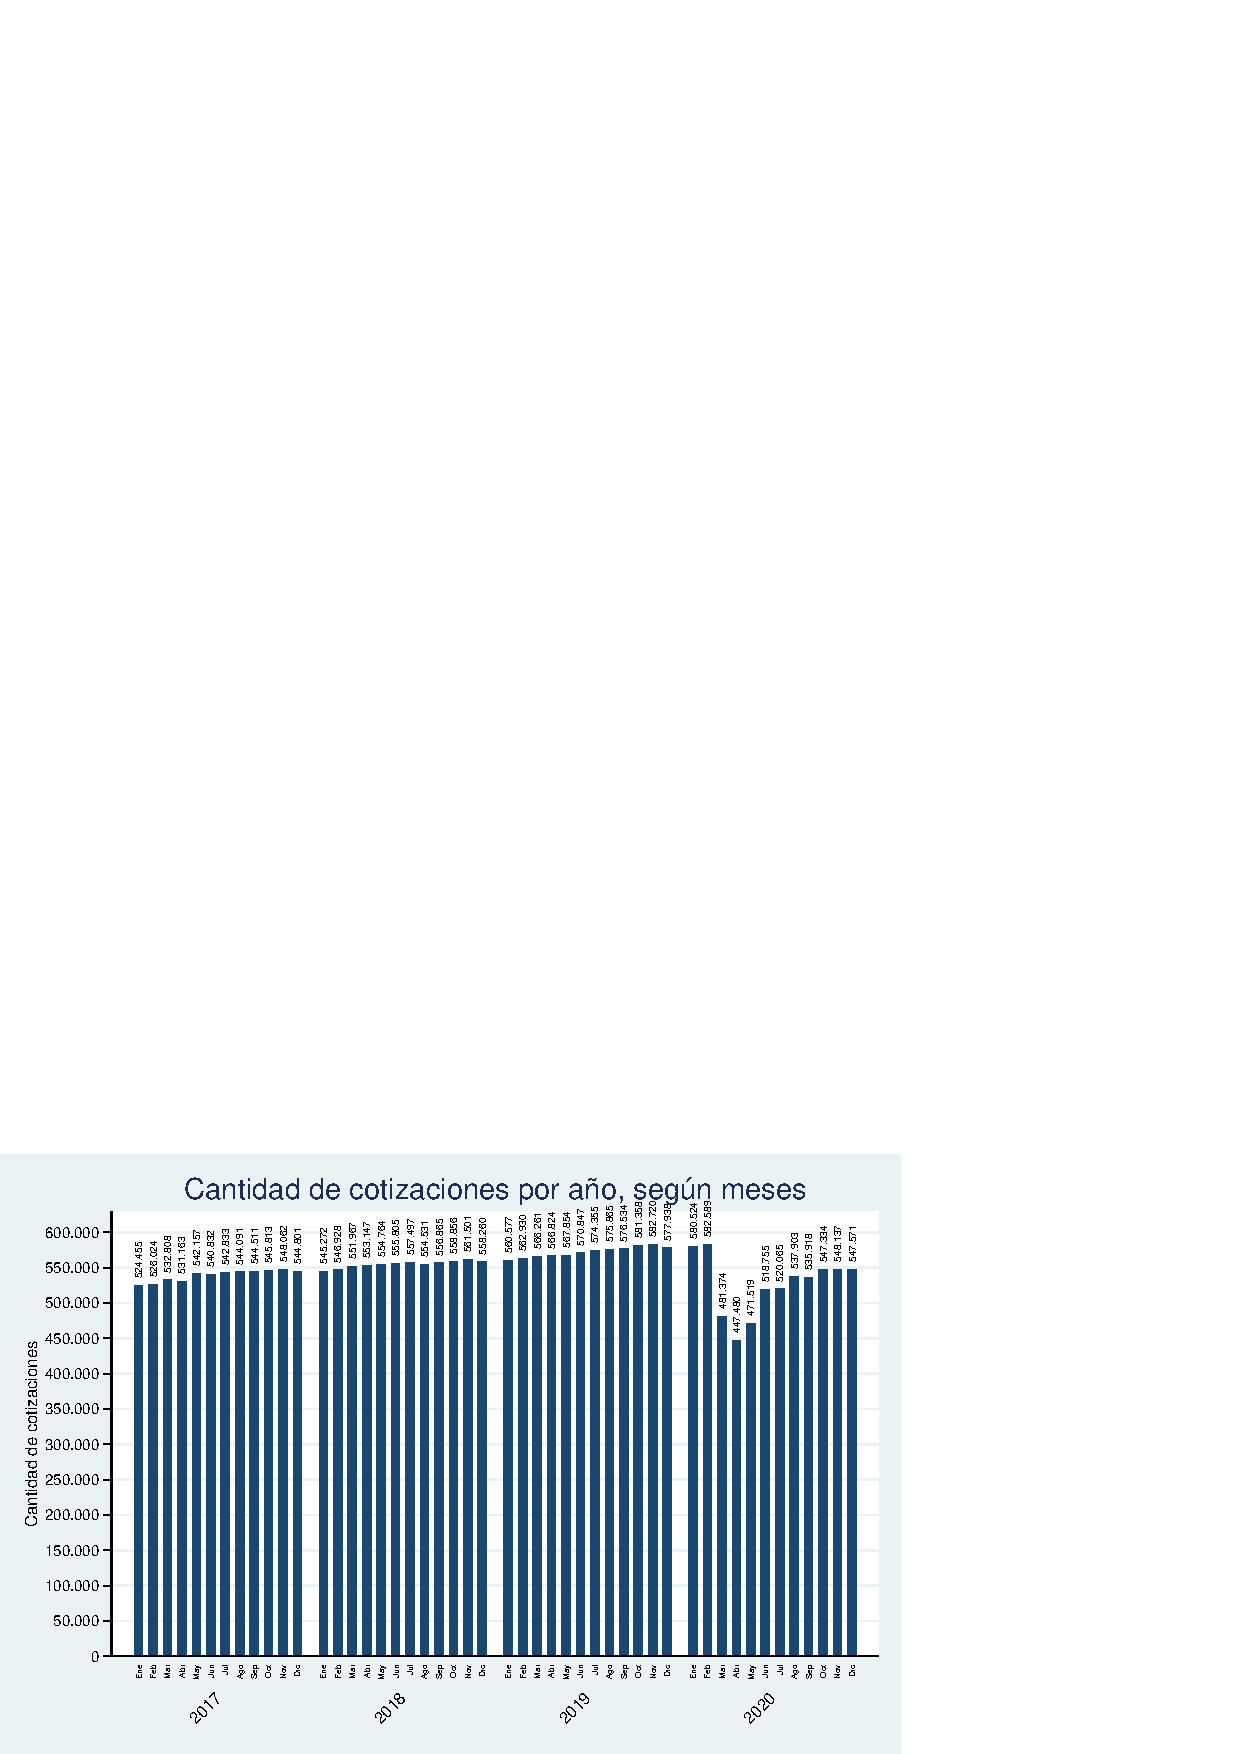
\includegraphics[scale=0.6]{RA_IPS_cotizaciones_puestos_2010a2020_mes.png}
\end{center}
\end{figure}

\begin{table}[H]
\begin{center}
\scriptsize     
\caption{\bf{Salario promedio por año y mes. (Puestos)}}
\begin{tabular}{l|rrrrrrrrrrrrr}
\input{RA_IPS_salprom_puestos_2010a2020_mes}
\end{tabular}
                    \item Fuente : Elaboración própia a partir de registros administrativos del IPS.
\end{center}
\end{table}

\begin{table}[H]
\begin{center}
\scriptsize     
\caption{\bf{Salario mediano por año y mes. (Puestos)}}
\begin{tabular}{l|rrrrrrrrrrrrr}
 & \multicolumn{13}{c}{\textbf{Mes}} \\
\textbf{Año}&\textbf{Ene}&\textbf{Feb}&\textbf{Mar}&\textbf{Abr}&\textbf{May}&\textbf{Jun}&\textbf{Jul}&\textbf{Ago}&\textbf{Sep}&\textbf{Oct}&\textbf{Nov}&\textbf{Dic}&\textbf{Total} \\
\hline
2010&1.409&1.409&1.409&1.409&1.409&1.409&1.508&1.508&1.508&1.508&1.508&1.508&1.508 \\
2011&1.508&1.508&1.508&1.658&1.658&1.658&1.658&1.658&1.658&1.658&1.658&1.658&1.658 \\
2012&1.658&1.658&1.658&1.658&1.658&1.658&1.658&1.659&1.658&1.658&1.658&1.658&1.659 \\
2013&1.658&1.658&1.658&1.658&1.659&1.658&1.659&1.659&1.659&1.659&1.658&1.658&1.659 \\
2014&1.659&1.658&1.824&1.824&1.824&1.824&1.824&1.825&1.824&1.825&1.824&1.824&1.825 \\
2015&1.824&1.824&1.824&1.824&1.825&1.825&1.825&1.825&1.825&1.825&1.824&1.824&1.825 \\
2016&1.824&1.824&1.824&1.824&1.825&1.825&1.824&1.825&1.825&1.825&1.827&1.965&1.965 \\
2017&1.965&1.965&1.978&1.978&1.985&2.000&2.042&2.061&2.044&2.052&2.050&2.066&2.066 \\
2018&2.078&2.064&2.086&2.100&2.127&2.109&2.157&2.189&2.162&2.187&2.165&2.183&2.189 \\
2019&2.187&2.163&2.197&2.200&2.222&2.200&2.254&2.270&2.253&2.268&2.250&2.259&2.270 \\
2020&2.251&2.229&2.193&2.193&2.282&2.269&2.274&2.283&2.263&2.283&2.267&2.313&2.313 \\
\textbf{Total}&2.251&2.229&2.197&2.200&2.282&2.269&2.274&2.283&2.263&2.283&2.267&2.313&2.313 \\

\end{tabular}
                    \item Fuente : Elaboración própia a partir de registros administrativos del IPS.
\end{center}
\end{table}

\begin{figure}[H]
\begin{center}
                    \caption{Salario promedio y mediano en los puestos por año y mes}
                    \vspace{0.5cm}
                    \includegraphics[scale=0.3]{RA_IPS_salprom_mediana_puestos_2010a2020_mes.png}
\end{center}
\end{figure}

\begin{table}[H]
\begin{center}
\scriptsize     
\caption{\bf{Distribución de los salarios respecto al SML (Julio de cada año)}}
\begin{tabular}{l|rrrrrrrrrrrrr}
\begin{tabular}{llllll}
\cline{1-6}
\multicolumn{1}{c}{} &
  \multicolumn{5}{|c}{Año} \\
\multicolumn{1}{c}{} &
  \multicolumn{1}{|r}{2016} &
  \multicolumn{1}{r}{2017} &
  \multicolumn{1}{r}{2018} &
  \multicolumn{1}{r}{2019} &
  \multicolumn{1}{r}{2020} \\
\cline{1-6}
\multicolumn{1}{r}{Monto del salarios nominal/SML} &
  \multicolumn{1}{|r}{} &
  \multicolumn{1}{r}{} &
  \multicolumn{1}{r}{} &
  \multicolumn{1}{r}{} &
  \multicolumn{1}{r}{} \\
\multicolumn{1}{r}{Menos de 1SML\hspace{1em}} &
  \multicolumn{1}{|r}{118.828} &
  \multicolumn{1}{r}{118.719} &
  \multicolumn{1}{r}{117.156} &
  \multicolumn{1}{r}{105.112} &
  \multicolumn{1}{r}{107.119} \\
\multicolumn{1}{r}{1 a menos de 2SML\hspace{1em}} &
  \multicolumn{1}{|r}{318.082} &
  \multicolumn{1}{r}{345.952} &
  \multicolumn{1}{r}{356.756} &
  \multicolumn{1}{r}{380.172} &
  \multicolumn{1}{r}{323.942} \\
\multicolumn{1}{r}{2 a menos de 3SML\hspace{1em}} &
  \multicolumn{1}{|r}{41.951} &
  \multicolumn{1}{r}{41.307} &
  \multicolumn{1}{r}{43.801} &
  \multicolumn{1}{r}{47.680} &
  \multicolumn{1}{r}{45.783} \\
\multicolumn{1}{r}{3 a menos de 4SML\hspace{1em}} &
  \multicolumn{1}{|r}{16.580} &
  \multicolumn{1}{r}{15.287} &
  \multicolumn{1}{r}{16.162} &
  \multicolumn{1}{r}{16.686} &
  \multicolumn{1}{r}{17.601} \\
\multicolumn{1}{r}{4 a menos de 5SML\hspace{1em}} &
  \multicolumn{1}{|r}{8.683} &
  \multicolumn{1}{r}{7.901} &
  \multicolumn{1}{r}{8.724} &
  \multicolumn{1}{r}{8.878} &
  \multicolumn{1}{r}{9.326} \\
\multicolumn{1}{r}{5 a menos de 6SML\hspace{1em}} &
  \multicolumn{1}{|r}{4.192} &
  \multicolumn{1}{r}{3.935} &
  \multicolumn{1}{r}{4.257} &
  \multicolumn{1}{r}{4.691} &
  \multicolumn{1}{r}{4.762} \\
\multicolumn{1}{r}{6 a menos de 7SML\hspace{1em}} &
  \multicolumn{1}{|r}{2.804} &
  \multicolumn{1}{r}{2.317} &
  \multicolumn{1}{r}{2.586} &
  \multicolumn{1}{r}{2.853} &
  \multicolumn{1}{r}{3.030} \\
\multicolumn{1}{r}{7 a menos de 8SML\hspace{1em}} &
  \multicolumn{1}{|r}{1.670} &
  \multicolumn{1}{r}{1.734} &
  \multicolumn{1}{r}{2.021} &
  \multicolumn{1}{r}{1.927} &
  \multicolumn{1}{r}{1.922} \\
\multicolumn{1}{r}{8 a menos de 9SML\hspace{1em}} &
  \multicolumn{1}{|r}{1.307} &
  \multicolumn{1}{r}{1.296} &
  \multicolumn{1}{r}{1.386} &
  \multicolumn{1}{r}{1.367} &
  \multicolumn{1}{r}{1.426} \\
\multicolumn{1}{r}{9 a menos de 10SML\hspace{1em}} &
  \multicolumn{1}{|r}{967} &
  \multicolumn{1}{r}{817} &
  \multicolumn{1}{r}{942} &
  \multicolumn{1}{r}{991} &
  \multicolumn{1}{r}{1.045} \\
\multicolumn{1}{r}{10SML y más\hspace{1em}} &
  \multicolumn{1}{|r}{4.101} &
  \multicolumn{1}{r}{3.568} &
  \multicolumn{1}{r}{3.706} &
  \multicolumn{1}{r}{3.998} &
  \multicolumn{1}{r}{4.109} \\
\multicolumn{1}{r}{Total\hspace{1em}} &
  \multicolumn{1}{|r}{519.165} &
  \multicolumn{1}{r}{542.833} &
  \multicolumn{1}{r}{557.497} &
  \multicolumn{1}{r}{574.355} &
  \multicolumn{1}{r}{520.065} \\
\cline{1-6}
\end{tabular}

\end{tabular}
                    \item Fuente : Elaboración própia a partir de registros administrativos del IPS.
\end{center}
\end{table}

\begin{table}[H]
\begin{center}
\scriptsize     
\caption{\bf{Distribución de los salarios respecto al SML (Julio de cada año, porcentajes)}}
\begin{tabular}{l|rrrrrrrrrrrrr}
\begin{tabular}{llllll}
\cline{1-6}
\multicolumn{1}{c}{} &
  \multicolumn{5}{|c}{Año} \\
\multicolumn{1}{c}{} &
  \multicolumn{1}{|r}{2016} &
  \multicolumn{1}{r}{2017} &
  \multicolumn{1}{r}{2018} &
  \multicolumn{1}{r}{2019} &
  \multicolumn{1}{r}{2020} \\
\cline{1-6}
\multicolumn{1}{r}{Monto del salarios nominal/SML} &
  \multicolumn{1}{|r}{} &
  \multicolumn{1}{r}{} &
  \multicolumn{1}{r}{} &
  \multicolumn{1}{r}{} &
  \multicolumn{1}{r}{} \\
\multicolumn{1}{r}{Menos de 1SML\hspace{1em}} &
  \multicolumn{1}{|r}{22,89\%} &
  \multicolumn{1}{r}{21,87\%} &
  \multicolumn{1}{r}{21,01\%} &
  \multicolumn{1}{r}{18,30\%} &
  \multicolumn{1}{r}{20,60\%} \\
\multicolumn{1}{r}{1 a menos de 2SML\hspace{1em}} &
  \multicolumn{1}{|r}{61,27\%} &
  \multicolumn{1}{r}{63,73\%} &
  \multicolumn{1}{r}{63,99\%} &
  \multicolumn{1}{r}{66,19\%} &
  \multicolumn{1}{r}{62,29\%} \\
\multicolumn{1}{r}{2 a menos de 3SML\hspace{1em}} &
  \multicolumn{1}{|r}{8,08\%} &
  \multicolumn{1}{r}{7,61\%} &
  \multicolumn{1}{r}{7,86\%} &
  \multicolumn{1}{r}{8,30\%} &
  \multicolumn{1}{r}{8,80\%} \\
\multicolumn{1}{r}{3 a menos de 4SML\hspace{1em}} &
  \multicolumn{1}{|r}{3,19\%} &
  \multicolumn{1}{r}{2,82\%} &
  \multicolumn{1}{r}{2,90\%} &
  \multicolumn{1}{r}{2,91\%} &
  \multicolumn{1}{r}{3,38\%} \\
\multicolumn{1}{r}{4 a menos de 5SML\hspace{1em}} &
  \multicolumn{1}{|r}{1,67\%} &
  \multicolumn{1}{r}{1,46\%} &
  \multicolumn{1}{r}{1,56\%} &
  \multicolumn{1}{r}{1,55\%} &
  \multicolumn{1}{r}{1,79\%} \\
\multicolumn{1}{r}{5 a menos de 6SML\hspace{1em}} &
  \multicolumn{1}{|r}{0,81\%} &
  \multicolumn{1}{r}{0,72\%} &
  \multicolumn{1}{r}{0,76\%} &
  \multicolumn{1}{r}{0,82\%} &
  \multicolumn{1}{r}{0,92\%} \\
\multicolumn{1}{r}{6 a menos de 7SML\hspace{1em}} &
  \multicolumn{1}{|r}{0,54\%} &
  \multicolumn{1}{r}{0,43\%} &
  \multicolumn{1}{r}{0,46\%} &
  \multicolumn{1}{r}{0,50\%} &
  \multicolumn{1}{r}{0,58\%} \\
\multicolumn{1}{r}{7 a menos de 8SML\hspace{1em}} &
  \multicolumn{1}{|r}{0,32\%} &
  \multicolumn{1}{r}{0,32\%} &
  \multicolumn{1}{r}{0,36\%} &
  \multicolumn{1}{r}{0,34\%} &
  \multicolumn{1}{r}{0,37\%} \\
\multicolumn{1}{r}{8 a menos de 9SML\hspace{1em}} &
  \multicolumn{1}{|r}{0,25\%} &
  \multicolumn{1}{r}{0,24\%} &
  \multicolumn{1}{r}{0,25\%} &
  \multicolumn{1}{r}{0,24\%} &
  \multicolumn{1}{r}{0,27\%} \\
\multicolumn{1}{r}{9 a menos de 10SML\hspace{1em}} &
  \multicolumn{1}{|r}{0,19\%} &
  \multicolumn{1}{r}{0,15\%} &
  \multicolumn{1}{r}{0,17\%} &
  \multicolumn{1}{r}{0,17\%} &
  \multicolumn{1}{r}{0,20\%} \\
\multicolumn{1}{r}{10SML y más\hspace{1em}} &
  \multicolumn{1}{|r}{0,79\%} &
  \multicolumn{1}{r}{0,66\%} &
  \multicolumn{1}{r}{0,66\%} &
  \multicolumn{1}{r}{0,70\%} &
  \multicolumn{1}{r}{0,79\%} \\
\multicolumn{1}{r}{Total\hspace{1em}} &
  \multicolumn{1}{|r}{100,00\%} &
  \multicolumn{1}{r}{100,00\%} &
  \multicolumn{1}{r}{100,00\%} &
  \multicolumn{1}{r}{100,00\%} &
  \multicolumn{1}{r}{100,00\%} \\
\cline{1-6}
\end{tabular}

\end{tabular}
                    \item Fuente : Elaboración própia a partir de registros administrativos del IPS.
\end{center}
\end{table}

\begin{figure}[H]
\begin{center}
                    \caption{Distribución de los salarios respecto al SML (Julio de cada año, porcentajes)}
                    \vspace{0.5cm}
                    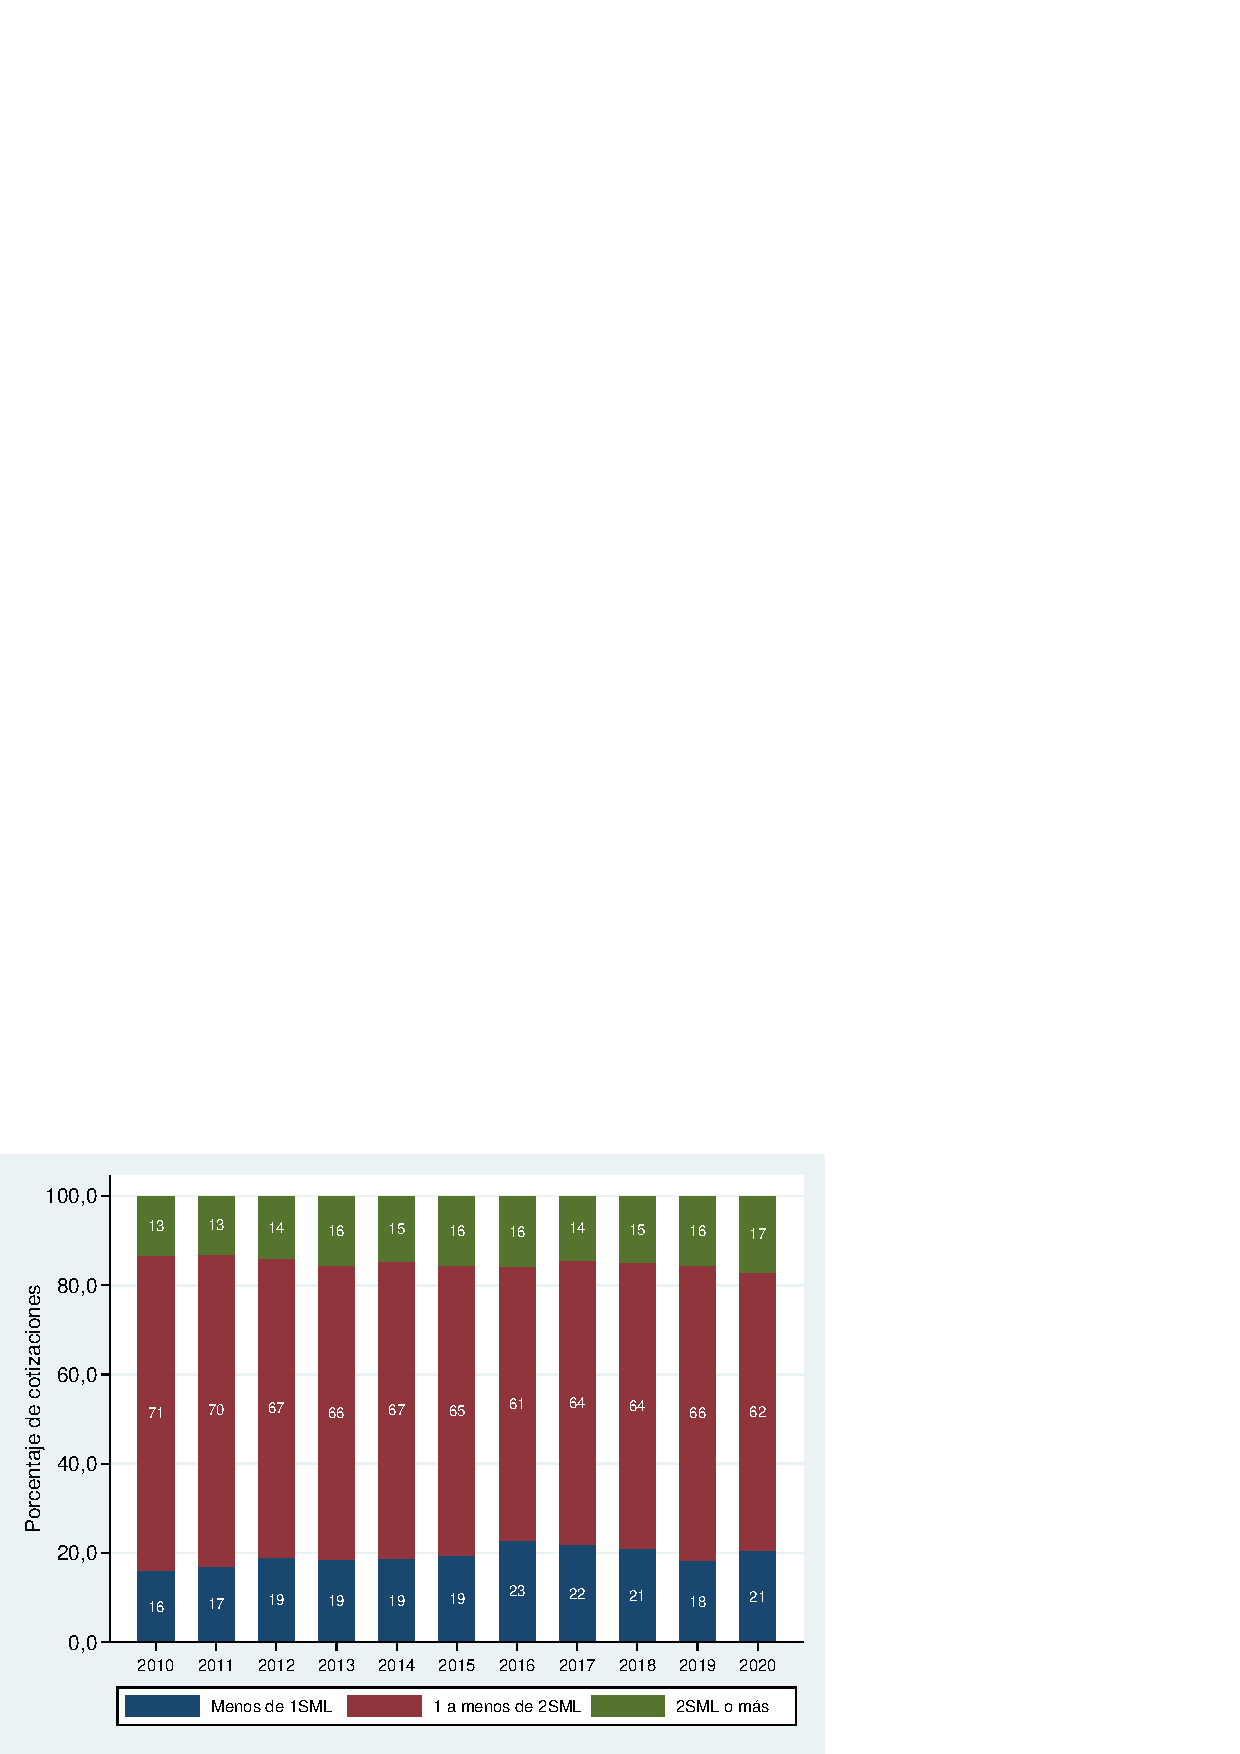
\includegraphics[scale=0.6]{RA_IPS_dist_salarial_puestos_2010a2020_mes_porcentajes.png}
\end{center}
\end{figure}

\begin{table}[H]
\begin{center}
\scriptsize     
\caption{\bf{Cantidad de cotizaciones por tipo de seguro y año (Julio de cada año, cantidades)}}
\begin{tabular}{l|rrrrrrrrrrrrr}
\begin{tabular}{lllllllll}
\cline{1-9}
\multicolumn{1}{c}{} &
  \multicolumn{8}{|c}{Año} \\
\multicolumn{1}{c}{} &
  \multicolumn{1}{|r}{2013} &
  \multicolumn{1}{r}{2014} &
  \multicolumn{1}{r}{2015} &
  \multicolumn{1}{r}{2016} &
  \multicolumn{1}{r}{2017} &
  \multicolumn{1}{r}{2018} &
  \multicolumn{1}{r}{2019} &
  \multicolumn{1}{r}{2020} \\
\cline{1-9}
\multicolumn{1}{l}{Tipo de seguro en el puesto} &
  \multicolumn{1}{|r}{} &
  \multicolumn{1}{r}{} &
  \multicolumn{1}{r}{} &
  \multicolumn{1}{r}{} &
  \multicolumn{1}{r}{} &
  \multicolumn{1}{r}{} &
  \multicolumn{1}{r}{} &
  \multicolumn{1}{r}{} \\
\multicolumn{1}{l}{\hspace{1em}Ama de Casa} &
  \multicolumn{1}{|r}{} &
  \multicolumn{1}{r}{43} &
  \multicolumn{1}{r}{83} &
  \multicolumn{1}{r}{89} &
  \multicolumn{1}{r}{94} &
  \multicolumn{1}{r}{94} &
  \multicolumn{1}{r}{88} &
  \multicolumn{1}{r}{76} \\
\multicolumn{1}{l}{\hspace{1em}Aprendices} &
  \multicolumn{1}{|r}{725} &
  \multicolumn{1}{r}{1.220} &
  \multicolumn{1}{r}{1.988} &
  \multicolumn{1}{r}{1.776} &
  \multicolumn{1}{r}{1.997} &
  \multicolumn{1}{r}{2.303} &
  \multicolumn{1}{r}{2.905} &
  \multicolumn{1}{r}{2.064} \\
\multicolumn{1}{l}{\hspace{1em}Continuidad en el Beneficio} &
  \multicolumn{1}{|r}{1.311} &
  \multicolumn{1}{r}{1.857} &
  \multicolumn{1}{r}{1.998} &
  \multicolumn{1}{r}{1.969} &
  \multicolumn{1}{r}{2.032} &
  \multicolumn{1}{r}{1.984} &
  \multicolumn{1}{r}{1.830} &
  \multicolumn{1}{r}{1.521} \\
\multicolumn{1}{l}{\hspace{1em}Chofer Cobrador} &
  \multicolumn{1}{|r}{645} &
  \multicolumn{1}{r}{665} &
  \multicolumn{1}{r}{853} &
  \multicolumn{1}{r}{1.195} &
  \multicolumn{1}{r}{1.189} &
  \multicolumn{1}{r}{1.289} &
  \multicolumn{1}{r}{1.318} &
  \multicolumn{1}{r}{1.028} \\
\multicolumn{1}{l}{\hspace{1em}Cotizante General} &
  \multicolumn{1}{|r}{320.164} &
  \multicolumn{1}{r}{342.603} &
  \multicolumn{1}{r}{360.068} &
  \multicolumn{1}{r}{372.044} &
  \multicolumn{1}{r}{395.870} &
  \multicolumn{1}{r}{412.060} &
  \multicolumn{1}{r}{424.563} &
  \multicolumn{1}{r}{381.110} \\
\multicolumn{1}{l}{\hspace{1em}Chofer de Omnibus} &
  \multicolumn{1}{|r}{571} &
  \multicolumn{1}{r}{677} &
  \multicolumn{1}{r}{665} &
  \multicolumn{1}{r}{719} &
  \multicolumn{1}{r}{693} &
  \multicolumn{1}{r}{643} &
  \multicolumn{1}{r}{633} &
  \multicolumn{1}{r}{384} \\
\multicolumn{1}{l}{\hspace{1em}Chofer a Inconstitucionalidad} &
  \multicolumn{1}{|r}{2.639} &
  \multicolumn{1}{r}{1.998} &
  \multicolumn{1}{r}{2.088} &
  \multicolumn{1}{r}{1.737} &
  \multicolumn{1}{r}{1.579} &
  \multicolumn{1}{r}{1.343} &
  \multicolumn{1}{r}{1.274} &
  \multicolumn{1}{r}{1.066} \\
\multicolumn{1}{l}{\hspace{1em}Jornalero a Destajo} &
  \multicolumn{1}{|r}{62.299} &
  \multicolumn{1}{r}{67.322} &
  \multicolumn{1}{r}{71.473} &
  \multicolumn{1}{r}{79.853} &
  \multicolumn{1}{r}{80.733} &
  \multicolumn{1}{r}{81.051} &
  \multicolumn{1}{r}{84.095} &
  \multicolumn{1}{r}{79.548} \\
\multicolumn{1}{l}{\hspace{1em}Cotizante Zafrero} &
  \multicolumn{1}{|r}{1.157} &
  \multicolumn{1}{r}{1.832} &
  \multicolumn{1}{r}{2.589} &
  \multicolumn{1}{r}{2.631} &
  \multicolumn{1}{r}{2.979} &
  \multicolumn{1}{r}{3.287} &
  \multicolumn{1}{r}{3.516} &
  \multicolumn{1}{r}{3.607} \\
\multicolumn{1}{l}{\hspace{1em}Doméstico Independiente} &
  \multicolumn{1}{|r}{} &
  \multicolumn{1}{r}{104} &
  \multicolumn{1}{r}{128} &
  \multicolumn{1}{r}{} &
  \multicolumn{1}{r}{} &
  \multicolumn{1}{r}{} &
  \multicolumn{1}{r}{} &
  \multicolumn{1}{r}{} \\
\multicolumn{1}{l}{\hspace{1em}Estibador Marítimo} &
  \multicolumn{1}{|r}{217} &
  \multicolumn{1}{r}{225} &
  \multicolumn{1}{r}{193} &
  \multicolumn{1}{r}{209} &
  \multicolumn{1}{r}{302} &
  \multicolumn{1}{r}{251} &
  \multicolumn{1}{r}{262} &
  \multicolumn{1}{r}{334} \\
\multicolumn{1}{l}{\hspace{1em}Empleadores} &
  \multicolumn{1}{|r}{} &
  \multicolumn{1}{r}{10} &
  \multicolumn{1}{r}{14} &
  \multicolumn{1}{r}{12} &
  \multicolumn{1}{r}{13} &
  \multicolumn{1}{r}{13} &
  \multicolumn{1}{r}{14} &
  \multicolumn{1}{r}{14} \\
\multicolumn{1}{l}{\hspace{1em}Ganadero tipo A} &
  \multicolumn{1}{|r}{8.454} &
  \multicolumn{1}{r}{8.783} &
  \multicolumn{1}{r}{9.148} &
  \multicolumn{1}{r}{9.443} &
  \multicolumn{1}{r}{9.270} &
  \multicolumn{1}{r}{8.735} &
  \multicolumn{1}{r}{9.140} &
  \multicolumn{1}{r}{8.876} \\
\multicolumn{1}{l}{\hspace{1em}Ganadero tipo B} &
  \multicolumn{1}{|r}{9.168} &
  \multicolumn{1}{r}{9.469} &
  \multicolumn{1}{r}{9.542} &
  \multicolumn{1}{r}{9.681} &
  \multicolumn{1}{r}{10.019} &
  \multicolumn{1}{r}{9.975} &
  \multicolumn{1}{r}{10.372} &
  \multicolumn{1}{r}{10.224} \\
\multicolumn{1}{l}{\hspace{1em}Cobrador y/o guarda} &
  \multicolumn{1}{|r}{100} &
  \multicolumn{1}{r}{125} &
  \multicolumn{1}{r}{122} &
  \multicolumn{1}{r}{142} &
  \multicolumn{1}{r}{128} &
  \multicolumn{1}{r}{108} &
  \multicolumn{1}{r}{101} &
  \multicolumn{1}{r}{52} \\
\multicolumn{1}{l}{\hspace{1em}Menores y Aprendices} &
  \multicolumn{1}{|r}{857} &
  \multicolumn{1}{r}{72} &
  \multicolumn{1}{r}{} &
  \multicolumn{1}{r}{} &
  \multicolumn{1}{r}{} &
  \multicolumn{1}{r}{} &
  \multicolumn{1}{r}{} &
  \multicolumn{1}{r}{} \\
\multicolumn{1}{l}{\hspace{1em}Menores} &
  \multicolumn{1}{|r}{101} &
  \multicolumn{1}{r}{196} &
  \multicolumn{1}{r}{174} &
  \multicolumn{1}{r}{120} &
  \multicolumn{1}{r}{123} &
  \multicolumn{1}{r}{106} &
  \multicolumn{1}{r}{84} &
  \multicolumn{1}{r}{74} \\
\multicolumn{1}{l}{\hspace{1em}Magisterio Privado} &
  \multicolumn{1}{|r}{17.701} &
  \multicolumn{1}{r}{17.849} &
  \multicolumn{1}{r}{18.163} &
  \multicolumn{1}{r}{18.316} &
  \multicolumn{1}{r}{18.108} &
  \multicolumn{1}{r}{18.038} &
  \multicolumn{1}{r}{18.663} &
  \multicolumn{1}{r}{15.437} \\
\multicolumn{1}{l}{\hspace{1em}Propietarios} &
  \multicolumn{1}{|r}{} &
  \multicolumn{1}{r}{5} &
  \multicolumn{1}{r}{7} &
  \multicolumn{1}{r}{7} &
  \multicolumn{1}{r}{8} &
  \multicolumn{1}{r}{10} &
  \multicolumn{1}{r}{12} &
  \multicolumn{1}{r}{9} \\
\multicolumn{1}{l}{\hspace{1em}Representantes del Empleador} &
  \multicolumn{1}{|r}{} &
  \multicolumn{1}{r}{5} &
  \multicolumn{1}{r}{6} &
  \multicolumn{1}{r}{7} &
  \multicolumn{1}{r}{10} &
  \multicolumn{1}{r}{8} &
  \multicolumn{1}{r}{9} &
  \multicolumn{1}{r}{11} \\
\multicolumn{1}{l}{\hspace{1em}Seguro Doméstico} &
  \multicolumn{1}{|r}{} &
  \multicolumn{1}{r}{} &
  \multicolumn{1}{r}{} &
  \multicolumn{1}{r}{18.889} &
  \multicolumn{1}{r}{17.319} &
  \multicolumn{1}{r}{15.827} &
  \multicolumn{1}{r}{15.148} &
  \multicolumn{1}{r}{8.679} \\
\multicolumn{1}{l}{\hspace{1em}Trabajadores Independientes} &
  \multicolumn{1}{|r}{} &
  \multicolumn{1}{r}{181} &
  \multicolumn{1}{r}{276} &
  \multicolumn{1}{r}{326} &
  \multicolumn{1}{r}{367} &
  \multicolumn{1}{r}{372} &
  \multicolumn{1}{r}{328} &
  \multicolumn{1}{r}{310} \\
\multicolumn{1}{l}{\hspace{1em}Tiempo Parcial} &
  \multicolumn{1}{|r}{} &
  \multicolumn{1}{r}{} &
  \multicolumn{1}{r}{} &
  \multicolumn{1}{r}{} &
  \multicolumn{1}{r}{} &
  \multicolumn{1}{r}{} &
  \multicolumn{1}{r}{} &
  \multicolumn{1}{r}{5.641} \\
\multicolumn{1}{l}{\hspace{1em}Total} &
  \multicolumn{1}{|r}{426.109} &
  \multicolumn{1}{r}{455.241} &
  \multicolumn{1}{r}{479.578} &
  \multicolumn{1}{r}{519.165} &
  \multicolumn{1}{r}{542.833} &
  \multicolumn{1}{r}{557.497} &
  \multicolumn{1}{r}{574.355} &
  \multicolumn{1}{r}{520.065} \\
\cline{1-9}
\end{tabular}

\end{tabular}
                    \item Fuente : Elaboración própia a partir de registros administrativos del IPS.
\end{center}
\end{table}

\begin{table}[H]
\begin{center}
\scriptsize     
\caption{\bf{Salario promedio por tipo de seguro y año (Julio de cada año, porcentajes)}}
\begin{tabular}{l|rrrrrrrrrrrrr}
\begin{tabular}{lllllllll}
\cline{1-9}
\multicolumn{1}{c}{} &
  \multicolumn{8}{|c}{Año} \\
\multicolumn{1}{c}{} &
  \multicolumn{1}{|r}{2013} &
  \multicolumn{1}{r}{2014} &
  \multicolumn{1}{r}{2015} &
  \multicolumn{1}{r}{2016} &
  \multicolumn{1}{r}{2017} &
  \multicolumn{1}{r}{2018} &
  \multicolumn{1}{r}{2019} &
  \multicolumn{1}{r}{2020} \\
\cline{1-9}
\multicolumn{1}{l}{Tipo de seguro en el puesto} &
  \multicolumn{1}{|r}{} &
  \multicolumn{1}{r}{} &
  \multicolumn{1}{r}{} &
  \multicolumn{1}{r}{} &
  \multicolumn{1}{r}{} &
  \multicolumn{1}{r}{} &
  \multicolumn{1}{r}{} &
  \multicolumn{1}{r}{} \\
\multicolumn{1}{l}{\hspace{1em}Ama de Casa} &
  \multicolumn{1}{|r}{} &
  \multicolumn{1}{r}{1.735.470} &
  \multicolumn{1}{r}{1.903.943} &
  \multicolumn{1}{r}{1.949.047} &
  \multicolumn{1}{r}{2.136.054} &
  \multicolumn{1}{r}{2.233.392} &
  \multicolumn{1}{r}{2.285.286} &
  \multicolumn{1}{r}{2.235.240} \\
\multicolumn{1}{l}{\hspace{1em}Aprendices} &
  \multicolumn{1}{|r}{1.653.246} &
  \multicolumn{1}{r}{1.575.525} &
  \multicolumn{1}{r}{1.573.089} &
  \multicolumn{1}{r}{1.388.009} &
  \multicolumn{1}{r}{1.656.406} &
  \multicolumn{1}{r}{1.879.165} &
  \multicolumn{1}{r}{1.938.421} &
  \multicolumn{1}{r}{2.137.402} \\
\multicolumn{1}{l}{\hspace{1em}Continuidad en el Beneficio} &
  \multicolumn{1}{|r}{3.249.500} &
  \multicolumn{1}{r}{3.414.139} &
  \multicolumn{1}{r}{3.546.595} &
  \multicolumn{1}{r}{3.812.223} &
  \multicolumn{1}{r}{4.130.066} &
  \multicolumn{1}{r}{4.548.354} &
  \multicolumn{1}{r}{4.898.909} &
  \multicolumn{1}{r}{4.892.697} \\
\multicolumn{1}{l}{\hspace{1em}Chofer Cobrador} &
  \multicolumn{1}{|r}{2.160.019} &
  \multicolumn{1}{r}{2.482.627} &
  \multicolumn{1}{r}{2.233.969} &
  \multicolumn{1}{r}{2.179.651} &
  \multicolumn{1}{r}{2.451.680} &
  \multicolumn{1}{r}{2.446.201} &
  \multicolumn{1}{r}{2.661.264} &
  \multicolumn{1}{r}{2.786.482} \\
\multicolumn{1}{l}{\hspace{1em}Cotizante General} &
  \multicolumn{1}{|r}{2.875.762} &
  \multicolumn{1}{r}{3.059.070} &
  \multicolumn{1}{r}{3.133.589} &
  \multicolumn{1}{r}{3.180.374} &
  \multicolumn{1}{r}{3.398.489} &
  \multicolumn{1}{r}{3.540.629} &
  \multicolumn{1}{r}{3.685.888} &
  \multicolumn{1}{r}{3.839.875} \\
\multicolumn{1}{l}{\hspace{1em}Chofer de Omnibus} &
  \multicolumn{1}{|r}{2.218.842} &
  \multicolumn{1}{r}{2.434.335} &
  \multicolumn{1}{r}{2.307.428} &
  \multicolumn{1}{r}{2.251.718} &
  \multicolumn{1}{r}{2.614.291} &
  \multicolumn{1}{r}{2.722.769} &
  \multicolumn{1}{r}{2.727.145} &
  \multicolumn{1}{r}{2.568.566} \\
\multicolumn{1}{l}{\hspace{1em}Chofer a Inconstitucionalidad} &
  \multicolumn{1}{|r}{2.078.803} &
  \multicolumn{1}{r}{2.353.808} &
  \multicolumn{1}{r}{2.229.077} &
  \multicolumn{1}{r}{2.147.926} &
  \multicolumn{1}{r}{2.398.288} &
  \multicolumn{1}{r}{2.493.070} &
  \multicolumn{1}{r}{2.768.052} &
  \multicolumn{1}{r}{2.573.789} \\
\multicolumn{1}{l}{\hspace{1em}Jornalero a Destajo} &
  \multicolumn{1}{|r}{1.754.919} &
  \multicolumn{1}{r}{1.858.612} &
  \multicolumn{1}{r}{1.864.311} &
  \multicolumn{1}{r}{1.867.158} &
  \multicolumn{1}{r}{2.087.503} &
  \multicolumn{1}{r}{2.229.835} &
  \multicolumn{1}{r}{2.279.792} &
  \multicolumn{1}{r}{2.313.656} \\
\multicolumn{1}{l}{\hspace{1em}Cotizante Zafrero} &
  \multicolumn{1}{|r}{2.054.868} &
  \multicolumn{1}{r}{2.062.367} &
  \multicolumn{1}{r}{2.204.650} &
  \multicolumn{1}{r}{2.459.558} &
  \multicolumn{1}{r}{2.802.903} &
  \multicolumn{1}{r}{2.694.971} &
  \multicolumn{1}{r}{2.905.446} &
  \multicolumn{1}{r}{2.766.485} \\
\multicolumn{1}{l}{\hspace{1em}Doméstico Independiente} &
  \multicolumn{1}{|r}{} &
  \multicolumn{1}{r}{778.525} &
  \multicolumn{1}{r}{801.069} &
  \multicolumn{1}{r}{} &
  \multicolumn{1}{r}{} &
  \multicolumn{1}{r}{} &
  \multicolumn{1}{r}{} &
  \multicolumn{1}{r}{} \\
\multicolumn{1}{l}{\hspace{1em}Estibador Marítimo} &
  \multicolumn{1}{|r}{702.527} &
  \multicolumn{1}{r}{720.739} &
  \multicolumn{1}{r}{755.431} &
  \multicolumn{1}{r}{749.536} &
  \multicolumn{1}{r}{1.679.438} &
  \multicolumn{1}{r}{2.159.302} &
  \multicolumn{1}{r}{1.176.313} &
  \multicolumn{1}{r}{1.115.608} \\
\multicolumn{1}{l}{\hspace{1em}Empleadores} &
  \multicolumn{1}{|r}{} &
  \multicolumn{1}{r}{1.942.244} &
  \multicolumn{1}{r}{2.818.752} &
  \multicolumn{1}{r}{3.282.152} &
  \multicolumn{1}{r}{3.609.252} &
  \multicolumn{1}{r}{3.590.446} &
  \multicolumn{1}{r}{3.547.957} &
  \multicolumn{1}{r}{2.492.192} \\
\multicolumn{1}{l}{\hspace{1em}Ganadero tipo A} &
  \multicolumn{1}{|r}{886.932} &
  \multicolumn{1}{r}{988.015} &
  \multicolumn{1}{r}{1.012.503} &
  \multicolumn{1}{r}{1.051.347} &
  \multicolumn{1}{r}{1.197.540} &
  \multicolumn{1}{r}{1.292.081} &
  \multicolumn{1}{r}{1.358.716} &
  \multicolumn{1}{r}{1.393.903} \\
\multicolumn{1}{l}{\hspace{1em}Ganadero tipo B} &
  \multicolumn{1}{|r}{1.475.131} &
  \multicolumn{1}{r}{1.624.327} &
  \multicolumn{1}{r}{1.670.776} &
  \multicolumn{1}{r}{1.741.572} &
  \multicolumn{1}{r}{1.841.931} &
  \multicolumn{1}{r}{2.008.215} &
  \multicolumn{1}{r}{2.104.973} &
  \multicolumn{1}{r}{2.150.600} \\
\multicolumn{1}{l}{\hspace{1em}Cobrador y/o guarda} &
  \multicolumn{1}{|r}{2.007.971} &
  \multicolumn{1}{r}{2.223.846} &
  \multicolumn{1}{r}{2.044.764} &
  \multicolumn{1}{r}{2.035.331} &
  \multicolumn{1}{r}{2.106.061} &
  \multicolumn{1}{r}{2.199.516} &
  \multicolumn{1}{r}{2.200.121} &
  \multicolumn{1}{r}{2.057.306} \\
\multicolumn{1}{l}{\hspace{1em}Menores y Aprendices} &
  \multicolumn{1}{|r}{1.129.532} &
  \multicolumn{1}{r}{1.596.349} &
  \multicolumn{1}{r}{} &
  \multicolumn{1}{r}{} &
  \multicolumn{1}{r}{} &
  \multicolumn{1}{r}{} &
  \multicolumn{1}{r}{} &
  \multicolumn{1}{r}{} \\
\multicolumn{1}{l}{\hspace{1em}Menores} &
  \multicolumn{1}{|r}{1.288.099} &
  \multicolumn{1}{r}{1.252.958} &
  \multicolumn{1}{r}{1.343.236} &
  \multicolumn{1}{r}{1.338.902} &
  \multicolumn{1}{r}{1.534.888} &
  \multicolumn{1}{r}{1.793.026} &
  \multicolumn{1}{r}{1.989.599} &
  \multicolumn{1}{r}{2.148.239} \\
\multicolumn{1}{l}{\hspace{1em}Magisterio Privado} &
  \multicolumn{1}{|r}{1.601.994} &
  \multicolumn{1}{r}{1.703.522} &
  \multicolumn{1}{r}{1.766.080} &
  \multicolumn{1}{r}{1.875.243} &
  \multicolumn{1}{r}{2.026.646} &
  \multicolumn{1}{r}{2.200.610} &
  \multicolumn{1}{r}{2.379.327} &
  \multicolumn{1}{r}{2.478.946} \\
\multicolumn{1}{l}{\hspace{1em}Propietarios} &
  \multicolumn{1}{|r}{} &
  \multicolumn{1}{r}{1.859.244} &
  \multicolumn{1}{r}{1.597.297} &
  \multicolumn{1}{r}{1.849.190} &
  \multicolumn{1}{r}{2.041.123} &
  \multicolumn{1}{r}{2.240.050} &
  \multicolumn{1}{r}{2.285.699} &
  \multicolumn{1}{r}{2.254.746} \\
\multicolumn{1}{l}{\hspace{1em}Representantes del Empleador} &
  \multicolumn{1}{|r}{} &
  \multicolumn{1}{r}{2.337.640} &
  \multicolumn{1}{r}{3.412.028} &
  \multicolumn{1}{r}{3.037.513} &
  \multicolumn{1}{r}{4.480.562} &
  \multicolumn{1}{r}{4.009.101} &
  \multicolumn{1}{r}{6.991.219} &
  \multicolumn{1}{r}{6.118.787} \\
\multicolumn{1}{l}{\hspace{1em}Seguro Doméstico} &
  \multicolumn{1}{|r}{} &
  \multicolumn{1}{r}{} &
  \multicolumn{1}{r}{} &
  \multicolumn{1}{r}{1.096.934} &
  \multicolumn{1}{r}{1.239.628} &
  \multicolumn{1}{r}{1.288.513} &
  \multicolumn{1}{r}{2.141.098} &
  \multicolumn{1}{r}{2.183.722} \\
\multicolumn{1}{l}{\hspace{1em}Trabajadores Independientes} &
  \multicolumn{1}{|r}{} &
  \multicolumn{1}{r}{1.885.546} &
  \multicolumn{1}{r}{2.039.887} &
  \multicolumn{1}{r}{2.053.929} &
  \multicolumn{1}{r}{2.515.378} &
  \multicolumn{1}{r}{2.636.275} &
  \multicolumn{1}{r}{3.108.561} &
  \multicolumn{1}{r}{3.016.326} \\
\multicolumn{1}{l}{\hspace{1em}Tiempo Parcial} &
  \multicolumn{1}{|r}{} &
  \multicolumn{1}{r}{} &
  \multicolumn{1}{r}{} &
  \multicolumn{1}{r}{} &
  \multicolumn{1}{r}{} &
  \multicolumn{1}{r}{} &
  \multicolumn{1}{r}{} &
  \multicolumn{1}{r}{1.184.705} \\
\multicolumn{1}{l}{\hspace{1em}Total} &
  \multicolumn{1}{|r}{2.574.125} &
  \multicolumn{1}{r}{2.743.639} &
  \multicolumn{1}{r}{2.803.244} &
  \multicolumn{1}{r}{2.773.901} &
  \multicolumn{1}{r}{3.007.139} &
  \multicolumn{1}{r}{3.163.804} &
  \multicolumn{1}{r}{3.313.859} &
  \multicolumn{1}{r}{3.414.990} \\
\cline{1-9}
\end{tabular}

\end{tabular}
                    \item Fuente : Elaboración própia a partir de registros administrativos del IPS.
\end{center}
\end{table}

\newpage
\subsubsection{Densidad de aportes}

La densidad promedio de aportes es calculada como el cociente entre la
cantidad total de activos que durante el año han aportado exactamente 1,
2, 3\ldots{}, 12 meses y el número de meses potencialmente aportados por
el total de asegurados, es decir una rela ción entre los aportes reales
y los potenciales.

Una mirada al Gráfico xx destaca que prácticamente no existen
diferencias por sexo entre el número de meses cotizados a lo largo del
periodo considerado, y se observa que alrededor del xx\% de hombres y
mujeres realizaron aportes los 12 meses del año 20 20.

El Gráfico xx evidencia que el número promedio de meses cotizados es
bajo para los tramos de edades más jóvenes, lo que podría explicarse por
una alta movilidad laboral, dedicación de tiempo parcial a los estudios
y/o informalidad laboral. En tanto aum enta la edad, el promedio del
número de meses de aportes también aumenta. Por otra parte, no se
aprecian diferencias por sexo en las edades inferiores a los 35 años. A
partir de dicha edad si se observa que existe un comportamiento
favorable para las m ujeres, en el sentido que, a medida que aumenta la
edad de las mujeres se incrementa el número promedio de meses cotizados
en el año.

\begin{table}[H]
\begin{center}
\footnotesize
\caption{\bf{Cantidad de cotizantes por la densidad de cotizaciones, según sexo}}
\begin{tabular}{l|rrrrrrrrrrr}
 & \multicolumn{6}{c}{\textbf{Sexo}} \\
\textbf{Densidad de cotizaciones (tramos)} & \multicolumn{2}{c}{\textbf{Hombres}} & \multicolumn{2}{c}{\textbf{Mujeres}} & \multicolumn{2}{c}{\textbf{Total}} \\
\hline
0 a 10\%&195.074&20,2943\%&105.347&19,1556\%&300.421&19,8799\% \\
11 a 19\%&113.505&11,8084\%&61.939&11,2626\%&175.444&11,6097\% \\
20 a 29\%&85.756&8,9215\%&47.615&8,6580\%&133.371&8,8256\% \\
30 a 39\%&67.369&7,0087\%&37.099&6,7458\%&104.468&6,9130\% \\
40 a 49\%&59.557&6,1959\%&32.900&5,9823\%&92.457&6,1182\% \\
50 a 59\%&61.792&6,4285\%&34.019&6,1858\%&95.811&6,3401\% \\
60 a 69\%&55.312&5,7543\%&31.534&5,7339\%&86.846&5,7469\% \\
70 a 79\%&54.536&5,6736\%&30.658&5,5746\%&85.194&5,6376\% \\
80 a 89\%&64.363&6,6959\%&38.704&7,0377\%&103.067&6,8203\% \\
90 a 99\%&117.156&12,1882\%&81.050&14,7376\%&198.206&13,1160\% \\
100\%&86.805&9,0307\%&49.089&8,9260\%&135.894&8,9926\% \\
\textbf{Total}&961.225&100,0000\%&549.954&100,0000\%&1.511.179&100,0000\% \\

\end{tabular}
                    \item \footnotesize Fuente : Elaboración própia a partir de registros administrativos del IPS.
                    \item \footnotesize Nota : 
\end{center}
\end{table}

\begin{figure}[H]
\begin{center}
                    \caption{Densidad de cotizaciones}
                    \vspace{0.5cm}
                    \includegraphics[scale=0.35]{dencot.png}
\end{center}
\end{figure}

\begin{figure}[H]
\begin{center}
                    \caption{Densidad de cotizaciones}
                    \vspace{0.5cm}
                    \includegraphics[scale=0.35]{dencot_by_sex}
\end{center}
\end{figure}

\newpage
\subsubsection{Nuevos beneficios pagados en Jubilaciones y Pensiones}

\subsubsection{Nuevos beneficios pagados en Jubilaciones y Pensiones}

Como ya se describió en la sección anterior ``Prestaciones'', el IPS
otorga diferentes tipos de beneficios en función a los riesgos que se
cubren. En la Tabla xx se observa la evolución de la cantidad de los
nuevos beneficios pagados por tipo (de benefic io) desde el año xx al
2020. Se destaca un crecimiento considerable en la cantidad de nuevos
beneficios concedidos entre dichos años con una variación interanual
promedio en torno al xx\%.

En el Gráfico xx se ilustra la evolución de los nuevos beneficios
pagados (altas) en J y P por tipo, y se puede apreciar claramente que
hubo aumentos en la concesión de Jubilaciones Ordinarias, acompañado a
su vez de la implementación de la Jubilación P roporcional que en el
primer año tuvo un inicio importante para luego ir disminuyendo
gradualmente. La cantidad de nuevos beneficios pagados por Pensiones
Derechohabiente y Jubilaciones por Invalidez, se mantuvieron
prácticamente constantes a lo largo d el periodo considerado.

El aumento en el número de nuevos beneficios pagados se entiende que se
debe no solo a una evolución esperada en el incremento de beneficios,
sino también a una gran mejoría en las gestiones administrativas para la
concesión de los beneficios llegando a otorgar el beneficio al momento
de cumplir el requisito de edad (Plan Retiro Feliz).

Al mismo tiempo, se pone de manifiesto que el comportamiento de los
nuevos beneficios otorgados por Jubilación Proporcional se debe a que,
al existir nuevos requisitos para acogerse a la Jubilación, muchas
personas con aportes entre 15 y 25 años pudiero n acceder a un
beneficio, que de otra manera hubiera sido imposible.

En la Gráfica xx se observa la distribución porcentual (pesos relativos)
de los diferentes tipos de beneficios. En referencia a esto, desde el
año 2008 hasta el año 2010 se ha tenido una distribución similar, siendo
las Pensiones Derechohabiente y la J ubilación Ordinaria las de mayor
peso relativo, en torno al 35\% y al 60\% respectivamente. A partir del
año 2011 se evidencia una caída en la distribución de los porcentajes,
la cual se ha visto alterada por la inclusión de la Ley 4290/11 de la
Jubilac ión Proporcional.

Es normal que en los primeros años que se ha introducido una
modificación en las condiciones para acceder a los beneficios de la
etapa pasiva, se observe una gran demanda que luego irá disminuyendo
hasta estabilizarse.

Tanto en la Tabla xx y en el Gráfico xx se aprecia claramente como en el
transcurso de los 10 últimos años, los montos (nominales) pagados por
Jubilación Ordinaria han tenido una tendencia creciente, hasta llegar a
un promedio de Gs.xx. Del mismo modo, los montos de los beneficios
otorgados por Jubilación Proporcional y Pensiones Derechohabiente han
ido aumentando entre los años 2015 y 2020 llegando en promedio a Gs.xx y
Gs.xx respectivamente. En tanto que, los montos promedios de las
Jubilaciones p or Invalidez presentan un pico en el año 2016, para
sufrir un leve descenso en el año 2017, llegando a un promedio de
Gs.2.245.444 param dicho año. En cuanto al Complemento al SML, el mismo
posee un comportamiento prácticamente constante en el periodo c
onsiderado y su valor promedio ronda los Gs.200.000.

La Tabla xx y el Gráfico xx presentan la distribución porcentual de la
cantidad de nuevos pagos en J y P de enero a diciembre del año 2020. Con
respecto a las Jubilaciones por Invalidez hay una demanda desde los 20
años, especialmente importante entre l os 45 y 65 años. La Jubilación
Ordinaria, por su parte presenta alrededor del xx\% de los nuevos pagos
en los dos primeros tramos etarios, aproximadamente el xx\% corresponde
a la Jubilación Ordinaria Anticipada concedida entre los 55 y 59 años de
edad y xx\% para la Ordinaria concedida a partir de los 60 años de edad.
Los nuevos pagos otorgados en concepto de Jubilación Proporcional, están
concentrados en el tramo de edad que va de los 65 a 69 años, alcanzando
aproximadamente el xx\%. Por último, los pagos por PDH se encuentran
distribuidos a lo largo de todos los tramos etarios, presentando mayores
frecuencias en algunos tramos particulares como se puede apreciar en la
Tabla xx.

\textbf{***agregar la tabla de porcentaje de nuevos beneficios pagados en jubilación por invalidez, jubilación ordinaria, jubilación proporcional y pensión de derechohabiente, según tramo de edad***}

\textbf{***agregar el gráfico de distribución de la edad de retiro por tipo de prestación***}

\begin{table}[H]
\begin{center}
\caption{\bf{Evolución de la cantidad de nuevos beneficios pagados en Jubilaciones y Pensiones.}}
\begin{tabular}{l|rrrrrrrrrrrrrrr}
\scriptsize
%\begin{tabular}{llllllllll}
\cline{1-10}
\multicolumn{1}{c}{} &
  \multicolumn{9}{|c}{Año de inicio de pago del beneficio} \\
\multicolumn{1}{c}{} &
  \multicolumn{1}{|r}{2012} &
  \multicolumn{1}{r}{2013} &
  \multicolumn{1}{r}{2014} &
  \multicolumn{1}{r}{2015} &
  \multicolumn{1}{r}{2016} &
  \multicolumn{1}{r}{2017} &
  \multicolumn{1}{r}{2018} &
  \multicolumn{1}{r}{2019} &
  \multicolumn{1}{r}{2020} \\
\cline{1-10}
\multicolumn{1}{l}{Clasificación del beneficio} &
  \multicolumn{1}{|r}{} &
  \multicolumn{1}{r}{} &
  \multicolumn{1}{r}{} &
  \multicolumn{1}{r}{} &
  \multicolumn{1}{r}{} &
  \multicolumn{1}{r}{} &
  \multicolumn{1}{r}{} &
  \multicolumn{1}{r}{} &
  \multicolumn{1}{r}{} \\
\multicolumn{1}{l}{\hspace{1em}Complemento SML} &
  \multicolumn{1}{|r}{996} &
  \multicolumn{1}{r}{936} &
  \multicolumn{1}{r}{739} &
  \multicolumn{1}{r}{579} &
  \multicolumn{1}{r}{541} &
  \multicolumn{1}{r}{677} &
  \multicolumn{1}{r}{587} &
  \multicolumn{1}{r}{485} &
  \multicolumn{1}{r}{1.125} \\
\multicolumn{1}{l}{\hspace{1em}Invalidéz Perm.} &
  \multicolumn{1}{|r}{86} &
  \multicolumn{1}{r}{70} &
  \multicolumn{1}{r}{73} &
  \multicolumn{1}{r}{91} &
  \multicolumn{1}{r}{163} &
  \multicolumn{1}{r}{104} &
  \multicolumn{1}{r}{108} &
  \multicolumn{1}{r}{101} &
  \multicolumn{1}{r}{100} \\
\multicolumn{1}{l}{\hspace{1em}Invalidéz Temp.} &
  \multicolumn{1}{|r}{249} &
  \multicolumn{1}{r}{273} &
  \multicolumn{1}{r}{242} &
  \multicolumn{1}{r}{265} &
  \multicolumn{1}{r}{323} &
  \multicolumn{1}{r}{289} &
  \multicolumn{1}{r}{292} &
  \multicolumn{1}{r}{286} &
  \multicolumn{1}{r}{199} \\
\multicolumn{1}{l}{\hspace{1em}Jub. Ordinaria} &
  \multicolumn{1}{|r}{1.986} &
  \multicolumn{1}{r}{2.181} &
  \multicolumn{1}{r}{2.407} &
  \multicolumn{1}{r}{2.518} &
  \multicolumn{1}{r}{2.784} &
  \multicolumn{1}{r}{2.848} &
  \multicolumn{1}{r}{2.714} &
  \multicolumn{1}{r}{2.989} &
  \multicolumn{1}{r}{3.073} \\
\multicolumn{1}{l}{\hspace{1em}Jub. Proporcional} &
  \multicolumn{1}{|r}{1.503} &
  \multicolumn{1}{r}{1.128} &
  \multicolumn{1}{r}{1.004} &
  \multicolumn{1}{r}{1.044} &
  \multicolumn{1}{r}{1.064} &
  \multicolumn{1}{r}{1.123} &
  \multicolumn{1}{r}{1.175} &
  \multicolumn{1}{r}{1.292} &
  \multicolumn{1}{r}{1.372} \\
\multicolumn{1}{l}{\hspace{1em}Pensión Derecho Hab.} &
  \multicolumn{1}{|r}{1.046} &
  \multicolumn{1}{r}{1.175} &
  \multicolumn{1}{r}{974} &
  \multicolumn{1}{r}{1.073} &
  \multicolumn{1}{r}{1.105} &
  \multicolumn{1}{r}{1.062} &
  \multicolumn{1}{r}{1.044} &
  \multicolumn{1}{r}{585} &
  \multicolumn{1}{r}{1.105} \\
\multicolumn{1}{l}{\hspace{1em}Jub. Continuidad} &
  \multicolumn{1}{|r}{} &
  \multicolumn{1}{r}{} &
  \multicolumn{1}{r}{} &
  \multicolumn{1}{r}{} &
  \multicolumn{1}{r}{} &
  \multicolumn{1}{r}{29} &
  \multicolumn{1}{r}{45} &
  \multicolumn{1}{r}{24} &
  \multicolumn{1}{r}{28} \\
\multicolumn{1}{l}{\hspace{1em}Jub. Intercajas} &
  \multicolumn{1}{|r}{} &
  \multicolumn{1}{r}{} &
  \multicolumn{1}{r}{} &
  \multicolumn{1}{r}{} &
  \multicolumn{1}{r}{} &
  \multicolumn{1}{r}{} &
  \multicolumn{1}{r}{} &
  \multicolumn{1}{r}{} &
  \multicolumn{1}{r}{3} \\
\multicolumn{1}{l}{\hspace{1em}Lo que en vida no percibió} &
  \multicolumn{1}{|r}{783} &
  \multicolumn{1}{r}{709} &
  \multicolumn{1}{r}{400} &
  \multicolumn{1}{r}{422} &
  \multicolumn{1}{r}{396} &
  \multicolumn{1}{r}{328} &
  \multicolumn{1}{r}{285} &
  \multicolumn{1}{r}{121} &
  \multicolumn{1}{r}{160} \\
\multicolumn{1}{l}{\hspace{1em}Indemnización} &
  \multicolumn{1}{|r}{14} &
  \multicolumn{1}{r}{20} &
  \multicolumn{1}{r}{10} &
  \multicolumn{1}{r}{12} &
  \multicolumn{1}{r}{17} &
  \multicolumn{1}{r}{37} &
  \multicolumn{1}{r}{69} &
  \multicolumn{1}{r}{72} &
  \multicolumn{1}{r}{56} \\
\multicolumn{1}{l}{\hspace{1em}Otro} &
  \multicolumn{1}{|r}{3} &
  \multicolumn{1}{r}{1} &
  \multicolumn{1}{r}{5} &
  \multicolumn{1}{r}{4} &
  \multicolumn{1}{r}{3} &
  \multicolumn{1}{r}{} &
  \multicolumn{1}{r}{} &
  \multicolumn{1}{r}{} &
  \multicolumn{1}{r}{} \\
\multicolumn{1}{l}{\hspace{1em}Total} &
  \multicolumn{1}{|r}{6.666} &
  \multicolumn{1}{r}{6.493} &
  \multicolumn{1}{r}{5.854} &
  \multicolumn{1}{r}{6.008} &
  \multicolumn{1}{r}{6.396} &
  \multicolumn{1}{r}{6.497} &
  \multicolumn{1}{r}{6.319} &
  \multicolumn{1}{r}{5.955} &
  \multicolumn{1}{r}{7.221} \\
\cline{1-10}
\end{tabular}

\end{tabular}
                    \item \footnotesize Fuente : Registros administrativos del IPS. 
                    \item \footnotesize Nota : Se refiere al salario promedio por puestos de trabajo que cotizaron al fondo de jubilaciones en cada mes.
\end{center}
\end{table}

\begin{figure}[H]
\begin{center}
\caption{Evolución de la cantidad de nuevos beneficios pagados por año}
%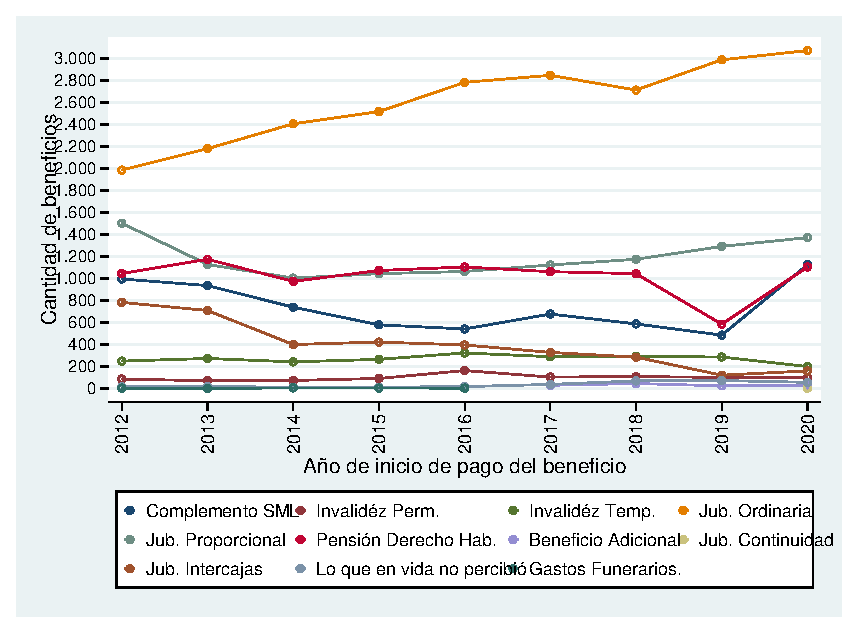
\includegraphics[scale=0.9]{RA_IPS_altas_clasif2_year.eps}
                    \item \footnotesize Fuente : Registros administrativos del IPS. 
                    \end{center}
\end{figure}

\textbf{***agregar el grafico de distribucion porcentual del total de nuebos beneficios pagados en J y P***}
\textbf{***agregar la tabla y el grafico de Evolucion del monto(nominal) promedio de los nuevos beneficios pagados en P y J***}

\subsubsection{Distribución de años de aportes}

El estudio de la cantidad de años de aportes con que se jubilan los
trabajadores y la densidad de aportes (años de aportes / años
trabajados) pone de manifiesto parte de la estructura de la movilidad
laboral, así como la entrada y salida del sistema, lo cual es sumamente
importante que sea representado adecuadamente en la construcción de un
modelo.

El Gráfico xx muestra como casi la mitad de los nuevos pagos por
Jubilaciones Ordinarias corresponden a trabajadores con 25 a 29 años de
antigüedad (xx\%), los restantes son trabajadores que se benefician con
la Jubilación Ordinaria concedida con al men os 30 años de antigüedad,
en tanto que, los nuevos pagos en Jubilaciones Proporcionales se dan en
un xx\% a trabajadores con 15 a 19 años de antigüedad. El xx\% restante
tiene 20 o más años de aportes acumulados. Por otra parte, en lo
concerniente a la Jubilación por Invalidez, no se requiere de ninguna
antigüedad, cuando se trata de accidentes de trabajo, por lo que se
observa una importante demanda en los trabajadores con pocos años de
antigüedad acumulados.

\textbf{***agregar gráfico de distribución porcentual de los nuevos beneficios pagados en jubilaciones por tipo de beneficio, según tramo de antiguedad***}

En el Gráfico xx se representan los nuevos beneficios pagados en
Jubilaciones Ordinarias (JO) en función a la edad de retiro y los años
de aportes (antigüedad), donde claramente se puede apreciar que la mayor
cantidad de personas accede al beneficio con los requisitos mínimos (60
años de edad y 25 años de aportes), y a partir de ahí le siguen las
personas que ya cuentan con uno de los requisitos (edad o antigüedad) y
acceden al beneficio una vez cumplido el segundo requisito.

\textbf{***agregar gráfico de cantidad de nuevos beneficios pagados en jubilación ordinaria por año de antigüedad, según tramos de edad***}

En los casos de Jubilaciones Ordinarias Anticipadas
(JOA)\footnote{La base de datos de Jubilaciones no distingue entre los conceptos de Jubilación Ordinaria y Jubilación Ordinaria Anticipada, la clasificación dada se ha conseguido mediante la revisión d
e las edades de retiro y los años de aporte para cada prestación.} ,
donde se requiere al menos 55 años de edad y 30 años de aportes, el
comportamiento es bastante similar cuando se los compara por edad de
retiro.

Un dato interesante es que, si bien el número es bajo, existen personas
que ya no desean o no pueden seguir aportando hasta la edad mínima
requerida (60 años) para obtener el 100\% de tasa de sustitución y se
retiran con años de aportes superiores a los 35 años (con al menos 55
años de edad).

En el caso de la Jubilación Proporcional no existe una clara tendencia
salvo que la mayor cantidad de beneficios se otorgaron a quienes
contaban con 15 años de antigüedad. Como la Ley entró en vigencia en el
año 2011, recién desde ese momento tuvieron oportunidad de acceder a un
beneficio las personas que contaban con la edad (65 años) pero no
llegaban al mínimo de 25 años de antigüedad (Ver Gráfico xx).

\textbf{agregar gráfico de cantidad de nuevos beneficios pagados en jubilación proporcional por ano de antigüedad, según tramos de edad}

\newpage
\subsubsection{Stock de Jubilaciones y Pensiones}

A diciembre del 2020, el IPS contaba con xx beneficios otorgados, de los
cuales el xx\% correspondían a Jubilación por Invalidez, el xx\% a
Jubilación Ordinaria, el xx\% a Jubilación Proporcional y el xx\% a
Pensiones (Ver Tabla xx).

El Gráfico xx ilustra la evolución del stock
\footnote{El término "stock" hace referencia a la cantidad total de beneficios pagados en J y P al último día de cada mes.  Los beneficios no incluyen el Complemento al SML ni los pagos por única vez (subsidi
os).} en J y P, en el cual se observa una tendencia creciente en los
beneficios otorgados en Jubilaciones Ordinarias y Jubilaciones
Proporcionales a lo largo de los últimos 5 años. En cuanto a las
Pensiones Derechohabiente y las Jubilaciones por Inval idez, la
tendencia revela estabilidad, es decir, se mantuvieron prácticamente
constantes a lo largo del intervalo estudiado.

Se aprecia en el Gráfico 3.14 que los montos nominales promedios del
stock de J y P, han tenido un incremento sostenido en los diferentes
tipos de prestaciones durante los últimos 5 años. Este aumento es
especialmente notorio en los pagos otorgados por Jubilaciones
Ordinarias, en donde se observa una suba de Gs. xxxxxxx entre los años
xx y xx, equivalente a un incremento del xx \%; seguido de los montos
por Jubilación Proporcional con un aumento del xx\%.

Por otra parte, las Jubilaciones por Invalidez y las Pensiones
Derechohabiente han tenido un incremento del xx\% y xx\%
respectivamente. En tanto que los Complementos al SML se han mantenido
sin grandes variaciones en el transcurso de dichos años.

\begin{table}[H]
\begin{center}
\caption{\bf{Evolución de la cantidad total beneficios pagados en Jubilaciones y Pensiones en el año 2020 (Stock).}}
\begin{tabular}{l|rrrrrrrrrrrrrrr}
\scriptsize
%\begin{tabular}{lllllllllllll}
\cline{1-13}
\multicolumn{1}{c}{} &
  \multicolumn{12}{|c}{Mes de pago} \\
\multicolumn{1}{c}{} &
  \multicolumn{1}{|r}{1} &
  \multicolumn{1}{r}{2} &
  \multicolumn{1}{r}{3} &
  \multicolumn{1}{r}{4} &
  \multicolumn{1}{r}{5} &
  \multicolumn{1}{r}{6} &
  \multicolumn{1}{r}{7} &
  \multicolumn{1}{r}{8} &
  \multicolumn{1}{r}{9} &
  \multicolumn{1}{r}{10} &
  \multicolumn{1}{r}{11} &
  \multicolumn{1}{r}{12} \\
\cline{1-13}
\multicolumn{1}{l}{Clasificación} &
  \multicolumn{1}{|r}{} &
  \multicolumn{1}{r}{} &
  \multicolumn{1}{r}{} &
  \multicolumn{1}{r}{} &
  \multicolumn{1}{r}{} &
  \multicolumn{1}{r}{} &
  \multicolumn{1}{r}{} &
  \multicolumn{1}{r}{} &
  \multicolumn{1}{r}{} &
  \multicolumn{1}{r}{} &
  \multicolumn{1}{r}{} &
  \multicolumn{1}{r}{} \\
\multicolumn{1}{l}{\hspace{1em}CSML} &
  \multicolumn{1}{|r}{7.890} &
  \multicolumn{1}{r}{12.139} &
  \multicolumn{1}{r}{12.253} &
  \multicolumn{1}{r}{12.172} &
  \multicolumn{1}{r}{12.186} &
  \multicolumn{1}{r}{12.289} &
  \multicolumn{1}{r}{12.596} &
  \multicolumn{1}{r}{12.677} &
  \multicolumn{1}{r}{12.698} &
  \multicolumn{1}{r}{12.725} &
  \multicolumn{1}{r}{12.718} &
  \multicolumn{1}{r}{12.754} \\
\multicolumn{1}{l}{\hspace{1em}JIP} &
  \multicolumn{1}{|r}{3.979} &
  \multicolumn{1}{r}{3.971} &
  \multicolumn{1}{r}{3.987} &
  \multicolumn{1}{r}{3.972} &
  \multicolumn{1}{r}{3.981} &
  \multicolumn{1}{r}{3.954} &
  \multicolumn{1}{r}{3.950} &
  \multicolumn{1}{r}{3.955} &
  \multicolumn{1}{r}{3.956} &
  \multicolumn{1}{r}{3.956} &
  \multicolumn{1}{r}{3.939} &
  \multicolumn{1}{r}{3.932} \\
\multicolumn{1}{l}{\hspace{1em}JIT} &
  \multicolumn{1}{|r}{339} &
  \multicolumn{1}{r}{334} &
  \multicolumn{1}{r}{331} &
  \multicolumn{1}{r}{298} &
  \multicolumn{1}{r}{296} &
  \multicolumn{1}{r}{289} &
  \multicolumn{1}{r}{293} &
  \multicolumn{1}{r}{281} &
  \multicolumn{1}{r}{284} &
  \multicolumn{1}{r}{281} &
  \multicolumn{1}{r}{258} &
  \multicolumn{1}{r}{261} \\
\multicolumn{1}{l}{\hspace{1em}JO} &
  \multicolumn{1}{|r}{37.531} &
  \multicolumn{1}{r}{37.510} &
  \multicolumn{1}{r}{37.761} &
  \multicolumn{1}{r}{37.726} &
  \multicolumn{1}{r}{37.968} &
  \multicolumn{1}{r}{38.104} &
  \multicolumn{1}{r}{38.329} &
  \multicolumn{1}{r}{38.436} &
  \multicolumn{1}{r}{38.530} &
  \multicolumn{1}{r}{38.705} &
  \multicolumn{1}{r}{38.704} &
  \multicolumn{1}{r}{38.790} \\
\multicolumn{1}{l}{\hspace{1em}JP} &
  \multicolumn{1}{|r}{10.112} &
  \multicolumn{1}{r}{10.168} &
  \multicolumn{1}{r}{10.265} &
  \multicolumn{1}{r}{10.278} &
  \multicolumn{1}{r}{10.375} &
  \multicolumn{1}{r}{10.472} &
  \multicolumn{1}{r}{10.592} &
  \multicolumn{1}{r}{10.685} &
  \multicolumn{1}{r}{10.780} &
  \multicolumn{1}{r}{10.886} &
  \multicolumn{1}{r}{10.922} &
  \multicolumn{1}{r}{10.986} \\
\multicolumn{1}{l}{\hspace{1em}BAA} &
  \multicolumn{1}{|r}{240} &
  \multicolumn{1}{r}{16} &
  \multicolumn{1}{r}{13} &
  \multicolumn{1}{r}{5} &
  \multicolumn{1}{r}{} &
  \multicolumn{1}{r}{} &
  \multicolumn{1}{r}{23} &
  \multicolumn{1}{r}{1} &
  \multicolumn{1}{r}{2} &
  \multicolumn{1}{r}{4} &
  \multicolumn{1}{r}{63.887} &
  \multicolumn{1}{r}{581} \\
\multicolumn{1}{l}{\hspace{1em}PDH} &
  \multicolumn{1}{|r}{13.663} &
  \multicolumn{1}{r}{13.627} &
  \multicolumn{1}{r}{13.646} &
  \multicolumn{1}{r}{13.576} &
  \multicolumn{1}{r}{13.556} &
  \multicolumn{1}{r}{13.563} &
  \multicolumn{1}{r}{13.688} &
  \multicolumn{1}{r}{13.828} &
  \multicolumn{1}{r}{13.878} &
  \multicolumn{1}{r}{13.961} &
  \multicolumn{1}{r}{13.967} &
  \multicolumn{1}{r}{14.076} \\
\multicolumn{1}{l}{\hspace{1em}JCON} &
  \multicolumn{1}{|r}{108} &
  \multicolumn{1}{r}{384} &
  \multicolumn{1}{r}{388} &
  \multicolumn{1}{r}{386} &
  \multicolumn{1}{r}{388} &
  \multicolumn{1}{r}{389} &
  \multicolumn{1}{r}{398} &
  \multicolumn{1}{r}{397} &
  \multicolumn{1}{r}{390} &
  \multicolumn{1}{r}{384} &
  \multicolumn{1}{r}{389} &
  \multicolumn{1}{r}{387} \\
\multicolumn{1}{l}{\hspace{1em}JINT} &
  \multicolumn{1}{|r}{} &
  \multicolumn{1}{r}{} &
  \multicolumn{1}{r}{12} &
  \multicolumn{1}{r}{12} &
  \multicolumn{1}{r}{12} &
  \multicolumn{1}{r}{13} &
  \multicolumn{1}{r}{13} &
  \multicolumn{1}{r}{13} &
  \multicolumn{1}{r}{13} &
  \multicolumn{1}{r}{13} &
  \multicolumn{1}{r}{15} &
  \multicolumn{1}{r}{14} \\
\multicolumn{1}{l}{\hspace{1em}LQVNP} &
  \multicolumn{1}{|r}{48} &
  \multicolumn{1}{r}{9} &
  \multicolumn{1}{r}{15} &
  \multicolumn{1}{r}{7} &
  \multicolumn{1}{r}{7} &
  \multicolumn{1}{r}{11} &
  \multicolumn{1}{r}{42} &
  \multicolumn{1}{r}{33} &
  \multicolumn{1}{r}{21} &
  \multicolumn{1}{r}{30} &
  \multicolumn{1}{r}{36} &
  \multicolumn{1}{r}{25} \\
\multicolumn{1}{l}{\hspace{1em}GF} &
  \multicolumn{1}{|r}{} &
  \multicolumn{1}{r}{} &
  \multicolumn{1}{r}{} &
  \multicolumn{1}{r}{} &
  \multicolumn{1}{r}{} &
  \multicolumn{1}{r}{} &
  \multicolumn{1}{r}{12} &
  \multicolumn{1}{r}{33} &
  \multicolumn{1}{r}{20} &
  \multicolumn{1}{r}{30} &
  \multicolumn{1}{r}{20} &
  \multicolumn{1}{r}{24} \\
\multicolumn{1}{l}{\hspace{1em}INDEM} &
  \multicolumn{1}{|r}{16} &
  \multicolumn{1}{r}{3} &
  \multicolumn{1}{r}{13} &
  \multicolumn{1}{r}{3} &
  \multicolumn{1}{r}{2} &
  \multicolumn{1}{r}{3} &
  \multicolumn{1}{r}{11} &
  \multicolumn{1}{r}{5} &
  \multicolumn{1}{r}{12} &
  \multicolumn{1}{r}{4} &
  \multicolumn{1}{r}{2} &
  \multicolumn{1}{r}{5} \\
\multicolumn{1}{l}{\hspace{1em}Otro} &
  \multicolumn{1}{|r}{2} &
  \multicolumn{1}{r}{} &
  \multicolumn{1}{r}{1} &
  \multicolumn{1}{r}{} &
  \multicolumn{1}{r}{} &
  \multicolumn{1}{r}{} &
  \multicolumn{1}{r}{} &
  \multicolumn{1}{r}{} &
  \multicolumn{1}{r}{} &
  \multicolumn{1}{r}{1} &
  \multicolumn{1}{r}{1} &
  \multicolumn{1}{r}{1} \\
\multicolumn{1}{l}{\hspace{1em}Total} &
  \multicolumn{1}{|r}{73.928} &
  \multicolumn{1}{r}{78.161} &
  \multicolumn{1}{r}{78.685} &
  \multicolumn{1}{r}{78.435} &
  \multicolumn{1}{r}{78.771} &
  \multicolumn{1}{r}{79.087} &
  \multicolumn{1}{r}{79.947} &
  \multicolumn{1}{r}{80.344} &
  \multicolumn{1}{r}{80.584} &
  \multicolumn{1}{r}{80.980} &
  \multicolumn{1}{r}{144.858} &
  \multicolumn{1}{r}{81.836} \\
\cline{1-13}
\end{tabular}

\end{tabular}
\end{center}
%\item \footnotesize Fuente : Registros administrativos del IPS.
\end{table}

Nota: CSML: Complemento por ajuste al 75\% del SML, JIP: Jubilación por
Invalidez Permanente, JIT: Jubilación por Invalidez Temporal, JO:
Jubilación Ordinaria, JP: Jubilación Proporcional, BAA: Beneficio
Adicional Anual, JCON:Jubilación por Convenios, J INT: Jubilación por
Intercajas, JNC-DP: Doc. Privados por Hacienda, LQVNP: Lo que en vida no
percibió, PDH: Pensión derechohabiente, Otro: Devolución por descuento
indebido, indemnización por nuevas nupcias, devolución de aportes,
indemnizaciones

\begin{table}[H]
\begin{center}
\caption{\bf{Evolución del monto promedio de los beneficios pagados en Jubilaciones y Pensiones en el año 2020 (Stock - En miles de Gs.).}}
\begin{tabular}{l|rrrrrrrrrrrrrrr}
\scriptsize
%\begin{tabular}{lllllllllllll}
\cline{1-13}
\multicolumn{1}{c}{} &
  \multicolumn{12}{|c}{Mes de pago} \\
\multicolumn{1}{c}{} &
  \multicolumn{1}{|r}{1} &
  \multicolumn{1}{r}{2} &
  \multicolumn{1}{r}{3} &
  \multicolumn{1}{r}{4} &
  \multicolumn{1}{r}{5} &
  \multicolumn{1}{r}{6} &
  \multicolumn{1}{r}{7} &
  \multicolumn{1}{r}{8} &
  \multicolumn{1}{r}{9} &
  \multicolumn{1}{r}{10} &
  \multicolumn{1}{r}{11} &
  \multicolumn{1}{r}{12} \\
\cline{1-13}
\multicolumn{1}{l}{Clasificación} &
  \multicolumn{1}{|r}{} &
  \multicolumn{1}{r}{} &
  \multicolumn{1}{r}{} &
  \multicolumn{1}{r}{} &
  \multicolumn{1}{r}{} &
  \multicolumn{1}{r}{} &
  \multicolumn{1}{r}{} &
  \multicolumn{1}{r}{} &
  \multicolumn{1}{r}{} &
  \multicolumn{1}{r}{} &
  \multicolumn{1}{r}{} &
  \multicolumn{1}{r}{} \\
\multicolumn{1}{l}{\hspace{1em}CSML} &
  \multicolumn{1}{|r}{331} &
  \multicolumn{1}{r}{495} &
  \multicolumn{1}{r}{493} &
  \multicolumn{1}{r}{493} &
  \multicolumn{1}{r}{493} &
  \multicolumn{1}{r}{493} &
  \multicolumn{1}{r}{492} &
  \multicolumn{1}{r}{484} &
  \multicolumn{1}{r}{481} &
  \multicolumn{1}{r}{479} &
  \multicolumn{1}{r}{478} &
  \multicolumn{1}{r}{478} \\
\multicolumn{1}{l}{\hspace{1em}JIP} &
  \multicolumn{1}{|r}{1.756} &
  \multicolumn{1}{r}{1.758} &
  \multicolumn{1}{r}{1.760} &
  \multicolumn{1}{r}{1.762} &
  \multicolumn{1}{r}{1.759} &
  \multicolumn{1}{r}{1.755} &
  \multicolumn{1}{r}{1.748} &
  \multicolumn{1}{r}{1.746} &
  \multicolumn{1}{r}{1.744} &
  \multicolumn{1}{r}{1.747} &
  \multicolumn{1}{r}{1.750} &
  \multicolumn{1}{r}{1.749} \\
\multicolumn{1}{l}{\hspace{1em}JIT} &
  \multicolumn{1}{|r}{2.158} &
  \multicolumn{1}{r}{2.201} &
  \multicolumn{1}{r}{2.221} &
  \multicolumn{1}{r}{2.204} &
  \multicolumn{1}{r}{2.330} &
  \multicolumn{1}{r}{2.299} &
  \multicolumn{1}{r}{2.296} &
  \multicolumn{1}{r}{2.313} &
  \multicolumn{1}{r}{2.226} &
  \multicolumn{1}{r}{2.176} &
  \multicolumn{1}{r}{2.363} &
  \multicolumn{1}{r}{2.317} \\
\multicolumn{1}{l}{\hspace{1em}JO} &
  \multicolumn{1}{|r}{4.453} &
  \multicolumn{1}{r}{4.474} &
  \multicolumn{1}{r}{4.487} &
  \multicolumn{1}{r}{4.506} &
  \multicolumn{1}{r}{4.517} &
  \multicolumn{1}{r}{4.537} &
  \multicolumn{1}{r}{4.551} &
  \multicolumn{1}{r}{4.561} &
  \multicolumn{1}{r}{4.575} &
  \multicolumn{1}{r}{4.580} &
  \multicolumn{1}{r}{4.597} &
  \multicolumn{1}{r}{4.608} \\
\multicolumn{1}{l}{\hspace{1em}JP} &
  \multicolumn{1}{|r}{1.800} &
  \multicolumn{1}{r}{1.811} &
  \multicolumn{1}{r}{1.820} &
  \multicolumn{1}{r}{1.823} &
  \multicolumn{1}{r}{1.830} &
  \multicolumn{1}{r}{1.837} &
  \multicolumn{1}{r}{1.847} &
  \multicolumn{1}{r}{1.851} &
  \multicolumn{1}{r}{1.855} &
  \multicolumn{1}{r}{1.867} &
  \multicolumn{1}{r}{1.870} &
  \multicolumn{1}{r}{1.876} \\
\multicolumn{1}{l}{\hspace{1em}BAA} &
  \multicolumn{1}{|r}{403} &
  \multicolumn{1}{r}{849} &
  \multicolumn{1}{r}{1.477} &
  \multicolumn{1}{r}{1.176} &
  \multicolumn{1}{r}{} &
  \multicolumn{1}{r}{} &
  \multicolumn{1}{r}{958} &
  \multicolumn{1}{r}{1.186} &
  \multicolumn{1}{r}{1.313} &
  \multicolumn{1}{r}{2.171} &
  \multicolumn{1}{r}{3.544} &
  \multicolumn{1}{r}{893} \\
\multicolumn{1}{l}{\hspace{1em}PDH} &
  \multicolumn{1}{|r}{1.540} &
  \multicolumn{1}{r}{1.537} &
  \multicolumn{1}{r}{1.539} &
  \multicolumn{1}{r}{1.541} &
  \multicolumn{1}{r}{1.545} &
  \multicolumn{1}{r}{1.546} &
  \multicolumn{1}{r}{1.547} &
  \multicolumn{1}{r}{1.545} &
  \multicolumn{1}{r}{1.546} &
  \multicolumn{1}{r}{1.548} &
  \multicolumn{1}{r}{1.550} &
  \multicolumn{1}{r}{1.553} \\
\multicolumn{1}{l}{\hspace{1em}JCON} &
  \multicolumn{1}{|r}{2.511} &
  \multicolumn{1}{r}{2.548} &
  \multicolumn{1}{r}{2.535} &
  \multicolumn{1}{r}{2.536} &
  \multicolumn{1}{r}{2.545} &
  \multicolumn{1}{r}{2.552} &
  \multicolumn{1}{r}{2.553} &
  \multicolumn{1}{r}{2.560} &
  \multicolumn{1}{r}{2.592} &
  \multicolumn{1}{r}{2.609} &
  \multicolumn{1}{r}{2.578} &
  \multicolumn{1}{r}{2.571} \\
\multicolumn{1}{l}{\hspace{1em}JINT} &
  \multicolumn{1}{|r}{} &
  \multicolumn{1}{r}{} &
  \multicolumn{1}{r}{1.187} &
  \multicolumn{1}{r}{1.187} &
  \multicolumn{1}{r}{1.187} &
  \multicolumn{1}{r}{1.107} &
  \multicolumn{1}{r}{1.107} &
  \multicolumn{1}{r}{1.107} &
  \multicolumn{1}{r}{1.107} &
  \multicolumn{1}{r}{1.107} &
  \multicolumn{1}{r}{1.150} &
  \multicolumn{1}{r}{1.222} \\
\multicolumn{1}{l}{\hspace{1em}LQVNP} &
  \multicolumn{1}{|r}{7.061} &
  \multicolumn{1}{r}{10.876} &
  \multicolumn{1}{r}{14.382} &
  \multicolumn{1}{r}{10.643} &
  \multicolumn{1}{r}{8.567} &
  \multicolumn{1}{r}{2.855} &
  \multicolumn{1}{r}{1.526} &
  \multicolumn{1}{r}{4.257} &
  \multicolumn{1}{r}{6.518} &
  \multicolumn{1}{r}{5.384} &
  \multicolumn{1}{r}{6.606} &
  \multicolumn{1}{r}{4.320} \\
\multicolumn{1}{l}{\hspace{1em}GF} &
  \multicolumn{1}{|r}{} &
  \multicolumn{1}{r}{} &
  \multicolumn{1}{r}{} &
  \multicolumn{1}{r}{} &
  \multicolumn{1}{r}{} &
  \multicolumn{1}{r}{} &
  \multicolumn{1}{r}{4.043} &
  \multicolumn{1}{r}{4.170} &
  \multicolumn{1}{r}{3.468} &
  \multicolumn{1}{r}{3.837} &
  \multicolumn{1}{r}{4.400} &
  \multicolumn{1}{r}{4.580} \\
\multicolumn{1}{l}{\hspace{1em}INDEM} &
  \multicolumn{1}{|r}{17.973} &
  \multicolumn{1}{r}{11.190} &
  \multicolumn{1}{r}{11.305} &
  \multicolumn{1}{r}{32.621} &
  \multicolumn{1}{r}{13.942} &
  \multicolumn{1}{r}{14.570} &
  \multicolumn{1}{r}{10.085} &
  \multicolumn{1}{r}{12.045} &
  \multicolumn{1}{r}{13.629} &
  \multicolumn{1}{r}{13.610} &
  \multicolumn{1}{r}{50.987} &
  \multicolumn{1}{r}{10.620} \\
\multicolumn{1}{l}{\hspace{1em}Otro} &
  \multicolumn{1}{|r}{251} &
  \multicolumn{1}{r}{} &
  \multicolumn{1}{r}{959} &
  \multicolumn{1}{r}{} &
  \multicolumn{1}{r}{} &
  \multicolumn{1}{r}{} &
  \multicolumn{1}{r}{} &
  \multicolumn{1}{r}{} &
  \multicolumn{1}{r}{} &
  \multicolumn{1}{r}{11.667} &
  \multicolumn{1}{r}{11.667} &
  \multicolumn{1}{r}{11.667} \\
\multicolumn{1}{l}{\hspace{1em}Total} &
  \multicolumn{1}{|r}{2.945} &
  \multicolumn{1}{r}{2.841} &
  \multicolumn{1}{r}{2.851} &
  \multicolumn{1}{r}{2.862} &
  \multicolumn{1}{r}{2.872} &
  \multicolumn{1}{r}{2.881} &
  \multicolumn{1}{r}{2.880} &
  \multicolumn{1}{r}{2.882} &
  \multicolumn{1}{r}{2.888} &
  \multicolumn{1}{r}{2.892} &
  \multicolumn{1}{r}{3.186} &
  \multicolumn{1}{r}{2.892} \\
\cline{1-13}
\end{tabular}

\end{tabular}
\end{center}
%\item \footnotesize Fuente : Registros administrativos del IPS. 
\end{table}

\newpage
\subsubsection{Relación Activos/ Pasivos en IPS}

Una variable muy utilizada como primer indicador de referencia para los
Sistemas Previsionales es la relación entre Activos y Pasivos. Los
países que cuentan con Sistemas Previsionales de Beneficio Definido
financiados mediante Reparto\footnote{Sistema 
de Reparto es también conocido como PAY-AS-YOU-GO.} monitorean con
rigurosos estudios actuariales que la promesa de pagar determinados
montos de haber previsional pueda ser cumplida, para lo cual es
sumamente importante contar con una gran cantidad de trabajadores
activos que sustenten a los jubilados y pensionados.

En términos simples, suponiendo que todos los trabajadores perciben la
misma remuneración y cada uno aporta el 20\% de su remuneración y se
pretende que el haber jubilatorio sea equivalente al 80\% del salario,
la cantidad de trabajadores por cada benef icio jubilatorio debe ser
igual a 4 (ya que con 20\% de la remuneración de cuatro aportantes se
puede financiar una jubilación equivalente al 80\% del salario
promedio).

Bajo el supuesto de que todos los trabajadores cotizantes al IPS
perciben la misma remuneración, y esta es igual o mayor al SML, se
necesitarían como mínimo 8 trabajadores activos para financiar la
jubilación de una persona que se retira percibiendo el 100\% del
promedio de sus últimas 36 remuneraciones, habiendo sido éstas iguales
al SML.

En la Tabla xx se aprecia la evolución anual de la relación entre la
cantidad de activos sobre la cantidad de pasivos que, en el caso del IPS
se ha mantenido muy alta y prácticamente constante durante los últimos 5
años. En este periodo dicha relación h a permanecido en torno a 11
activos por cada pasivo. El Gráfico xx ilustra la evolución de este
indicador y muestra con mayor claridad la tendencia, principalmente
caracterizada por una leve disminución observada en los 5 años
analizados.

Precisamente en el mes de noviembre del año 2015 fueron incorporados al
Régimen General los trabajadores domésticos, lo que produjo un aumento
cercano al 4\% en la cantidad de cotizantes (aproximadamente 20.000
trabajadores). Sin embargo, esta incorpora ción de nuevos cotizantes no
se mantuvo en los años posteriores, pues como puede notarse, la relación
volvió a descender a los niveles anteriormente observados. Cabe señalar
que, este indicador muestra la relación bruta, ya que no tiene en cuenta
el por centaje de aporte, ni los salarios, ni los niveles de haber
jubilatorio.

\textbf{***agregarla tabla de Relación entre la cantidad de trabajadores activos y pasivos y entre los salarios y beneficios promedios***}

\textbf{***agregar el gráfico Evolución anual de la cantidad de activos sobre pasivos***}

A su vez, en la misma Tabla xx se puede observar la evolución de la
relación entre el salario promedio del trabajador activo y el monto
promedio de los beneficios pagados en J y P. En el año 2013 la relación
era de 1,31; es decir el salario promedio del activo era 31\% superior
respecto al beneficio promedio del pasivo. Para el año 2020 esta
relación disminuyó a xx lo cual puede interpretarse como un acercamiento
sustancial entre el salario promedio y el beneficio promedio. La
tendencia queda ilustrad a en el Gráfico xx y deja claro cómo los
beneficios promedios aumentan a un ritmo mayor que los salarios
promedios. Desde otro enfoque, esto implica que los beneficios promedios
pasaron de representar un 76\% a un 87\% del salario promedio del activo
en un periodo de 5 años.

\textbf{***agregar el gráfico Evolución anual del salario medio del activo sobre el beneficio medio del pasivo***}

\newpage
%\input{projact_caterainver}
%\newpage
%\input{projact_}
%\newpage
%\input{projact_}
%\newpage
%\input{projact_}
%\newpage
%\input{projact_}












\subsection{Cobertura del IPS}

Considerando la cobertura del IPS sobre la población total ocupada se puede ver en la figura 46 que la tasa presenta un incremento lento y sostenido pasando del 21,3\% en 2018 a 28,5\% en el año 2100.  Así también se puede apreciar la cobertura sobre la PEA y en este caso la tasa pasa del 20,2\% al 27,2\% para el mismo lapso de tiempo.

Se debe tener en cuenta que la población objetivo del IPS son sólo los trabajadores del sector privado en relación de dependencia, y no todos los trabajadores ocupados, por tanto, la tasa de cobertura sobre la Población Total Ocupada Dependiente entre 15 a 69 años de edad (asalariados del Sector Privado y trabajadores domésticos) se comporta de manera similar, pero con valores superiores, pasando del 41,5\% al 55,3\% para el final de la proyección.

\textbf{falta el gráfico de Proyección de la Tasa de Cobertura del IPS}

En el año 2018 se registra un total de 701.607 cotizantes entre 15 y 69 años de edad, de los cuales 446.310 (63,6\%) son hombres y 255.297 (36,4\%) son mujeres. Para el año 2100 se proyecta que la cantidad total de aportantes en el mismo rango de edad ascienda a 1.775.795 personas, de los cuales 1.051.229 (59,2\%) serán hombres y 724.566 mujeres (40,8\%) (ver Gráfico x).

\textbf{falta el gráfico Proyección de la cantidad de aportantes}


Se estima que el IPS contará con un total de aproximadamente 65.500 beneficios de Jubilaciones y Pensiones pagados en el mes de diciembre del año 2018 y según los resultados de la proyección se espera que esta cantidad ascienda a casi 500.000 pagos para el año 2100. 

\textbf{falta el gráfico Proyección de la cantidad de Beneficios}

En el Gráfico x se puede observar la proyección del peso o participación que representa cada tipo de beneficio en el total de jubilaciones y pensiones pagadas en diciembre de cada año. Resulta notable el cambio importante observado en la gráfica, donde los porcentajes varían principalmente dentro de los primeros 20 años de proyección, para luego alcanzar cierta estabilidad hasta el final de la proyección. Para el año base, los beneficios JON, JOA, JP, JI y PDH representaban 66, 7, 4, 7 y 17 pagos respectivamente por cada 100, y para el final de la proyección se espera que esta distribución cambie a 36, 20, 4, 4 y 35 de cada 100 pagos. De esta manera los aumentos más importantes, se espera ocurran en la PDH y la JOA. 

\textbf{falta le gráfico Peso relativo según tipo de Beneficio}

\subsubsection{Altas de beneficios anuales}

La proyección de la cantidad de altas por año se presenta en el Gráfico x donde para el año 2018 se espera que el IPS cuente con aproximadamente 5.800 nuevos pagos otorgados en beneficios de Jubilaciones y Pensiones\footnote{Las pensiones incluyen los pagos periódicos de pensión por viudez y los pagos de orfandad.} . La Jubilación Ordinaria y las de Pensiones son las que presentan el aumento más importante en términos absolutos, mientras que la Jubilación Ordinaria Anticipada, la Proporcional y la de Invalidez presentan aumentos más moderados. Para el año 2100 se espera contar con aproximadamente 22.000 nuevos pagos en el año.

\textbf{falta el gráfico Proyección de la cantidad de nuevos beneficios (altas) pagados en Jubilaciones y Pensiones}

\subsubsection{Proyección Relación Aporte/Beneficio}

Como ya se mencionó en el Capítulo III “Situación Actual del IPS”, un importante indicador obtenido es la relación entre la cantidad de aportantes y la cantidad de beneficios otorgados. En el año 2018 este indicador tendrá un valor de 10,7\footnote{Este valor es obtenido de la base de datos de activos y pasivos y el mismo difiere del valor publicado oficialmente por la Dirección de Aportes, debido a que las definiciones aplicadas para las proyecciones de los activos solo incluyen a las edades entre 15 y 69 años} , lo que significa que había aproximadamente 11 aportantes por cada beneficio otorgado. Según los resultados este valor tendrá una disminución lenta hasta llegar a un valor de 3,6 en el final de la proyección.

\textbf{falta el grafico Proyección de la relación Aportantes/Beneficios}

\subsection{Resultados Financieros}

Uno de los objetivos del presente trabajo es que las proyecciones se basen en las condiciones actuales del Sistema Jubilatorio del IPS, por lo que en vez de utilizar un modelo de proyecciones general, se ha realizado los módulos necesarios para representar los principales casos de beneficios (Jubilación Ordinaria, Jubilación Ordinaria Anticipada, Jubilación Proporcional, Pensión por Invalidez, Pensión Derechohabiente).

Con el propósito de presentar un modelo de proyecciones lo más cercano a la realidad, se expondrán primeramente los resultados del “Escenario Base sin Aporte Estatal”, donde se consideran 12 pagos mensuales de Jubilaciones y Pensiones, y seguidamente un “Escenario Base con Aporte Estatal” (básicamente lo estipulado en la legislación actual, pero no implementado).

Así también, si bien la legislación contempla el pago de un Beneficio Adicional Anual (decimotercer haber jubilatorio o mal llamado aguinaldo), este depende de que los cálculos actuariales y las posibilidades financieras y presupuestarias lo permitan, y finalmente de la decisión del Consejo de Administración (por mayoría absoluta de los miembros) para ser pagado.  Por tal motivo se consideran escenarios alternativos de “Escenario con Pago BAA” con y sin Aporte Estatal.

Seguidamente se analizará la proyección de Ingresos, posteriormente la proyección de Egresos y finalmente la proyección del Resultado Corriente.

\subsubsection{Recaudaciòn (Aporte Obrero - Patronal)}

Para el cálculo de las recaudaciones Obrero-Patronales se considera la masa salarial total con 12 salarios proyectada y se le aplica la alícuota del 12,5\%, obteniéndose así los ingresos por recaudación. Los resultados se representan en el Gráfico x donde se observa que la recaudación va desde el 1,41\% del PIB en el 2018 a un 1,97\% del PIB en el 2100.

Mientras que, si se considera una masa salarial total con 13 sueldos, la recaudación aumenta al 1,53\% y 2,13\% del PIB para el 2018 y 2100 respectivamente.  La alternativa de 13 sueldos se plantea para analizar el impacto de financiar el BAA con aportes sobre el aguinaldo (hoy día la legislación vigente no lo permite).

\textbf{falta el gráfico Recaudación según Masa Salarial (en \% del PIB)}

En el gráfico precedente se puede apreciar que el crecimiento en la recaudación se proyecta lento pero sostenido si se lo toma en términos relativos al Producto Interno Bruto, es decir, en porcentajes, mientras que al proyectarlo en valores absolutos (Gráfico x) se aprecia un incremento mayor a partir de la segunda mitad del periodo bajo consideración.

\textbf{falta el gráfico Recaudación según Masa Salarial (valores nominales)}

\subsubsection{Egresos por prestaciones}

El gasto en prestaciones, para el año 2018 se proyecta en 1,05\% del PIB, aumentando en forma paulatina y sostenida durante todos los años de la proyección, llegando al año 2100 a un 3,64\% del PIB.

\textbf{falta el gráfico Egresos por Jubilaciones y Pensiones}

Similar al comportamiento de los Ingresos, cuando se consideran los Egresos en términos nominales, el incremento en la segunda mitad se comienza a acelerar.

\textbf{falta el gráfico Egresos por Jubilaciones y Pensiones}

Con respecto a la composición del gasto, se puede ver en el Gráfico x, que en el año 2018 las Jubilaciones de Vejez, Pensiones por Derechohabiente y por Jubilaciones por Invalidez representan 87\%, 9\% y 4\% del gasto total respectivamente. Según los resultados de la proyección, el peso de las Jubilaciones tendrá un descenso sostenido en los primeros 20 años de proyección para luego estabilizarse en un valor de 72\% del gasto total. En contrapartida, las Pensiones y las Invalideces experimentarán un aumento sostenido durante el mismo lapso de tiempo para luego estabilizarse en un 24\% y 3\% respectivamente.

\textbf{falta el gráfico Composición del gasto según tipo de Beneficio}

El gasto en prestaciones con respecto a la masa de aportes se proyecta en un valor aproximado del 74\% para el año 2018, este valor experimentará un aumento sostenido hasta aproximadamente el año 2044, donde los gastos ya alcanzan el 100\% de la masa de aportes.  La tendencia a continuación es de un aumento hasta el final de la proyección alcanzando un valor del 149\%

\textbf{falta el grafico Gastos por prestaciones (en \% de la Masa Salarial Imponible)}

Queda claro que el porcentaje de aporte al Sistema de Jubilaciones es superior al requerido si se lo considera como un sistema de reparto puro, por lo que la diferencia va generando un Fondo que será utilizado cuando los aportes obrero-patronales ya no sean suficientes para hacer frente a las erogaciones.

En el Gráfico x se representa cómo evolucionaría la tasa de aporte al Sistema Jubilatorio si fuera un sistema de reparto puro con actualización de la tasa al final de cada año para mantener el equilibrio financiero del sistema.

\textbf{falta el gráfico Gastos sobre la Masa Salarial Imponible}

Se puede apreciar que en el año 2044 se alcanzaría un equilibrio con 12,4\% de aportes sobre los salarios, a partir de ese año los aportes ya no serían suficientes y para el año 2067 se requeriría que la misma sea del 18,6\%.

\subsubsection{Resultado corriente}

El Resultado Corriente es la diferencia entre las proyecciones de Ingresos (aportes obrero-patronales sin considerar las ganancias por la rentabilidad del Fondo) y Egresos (prestaciones por Jubilaciones y Pensiones).

En el Gráfico x se representan las proyecciones de Ingresos y Egresos en relación al PIB, donde se puede apreciar que las líneas se cruzan en el año 2044, quedando claro que existe un Superávit y posterior al mismo año un Déficit Corriente.

\textbf{falta el grafico Ingresos y Egresos por Jubilaciones y Pensiones}

En el Gráfico x puede apreciarse los resultados de la proyección de los Ingresos y Egresos contrastando el efecto de la inclusión del Aporte Estatal. En el año 2018 los Egresos representan el 1,05\% del PIB, experimentando luego un aumento sostenido hasta el final de la proyección, donde alcanza un valor que representará el 3,64\% del PIB. 

Se resaltan dos puntos de interés en el gráfico, el primero indica el punto de coincidencia entre los Ingresos y los Egresos (sin el pago del BAA) en el año 2044 con un valor de los Egresos del 1,67\% del PIB. El otro punto de interés indica cuando se cruzan las líneas de los Ingresos (considerando el aporte del estado) y los Egresos, el cual se sitúa en el año 2050, alcanzando los egresos en este punto un 1,94\% del PIB.

\textbf{falta el gráfico Resultado corriente (con y sin aporte estatal)}

En el Gráfico x se representa la Evolución del Resultado Corriente con (RCcAE) y sin Aporte Estatal (RCsAE) (1,5\% sobre los salarios), donde se puede apreciar que se parte de actual Superávit de 0,36\% RCsAE y 0,53\% RCcAE, para llegar a un Déficit del 0,68\% y 0,90\% respectivamente en el año 2067.  El hecho de no contar con el Aporte Estatal genera que el Déficit Corriente se adelante 6 años.

\textbf{falta el grafico Resultado corriente con y sin aporte estatal (recaudación - prestaciones)}

\subsubsection{Fondo de Reserva}

Está claro que como actualmente existe un Superávit Corriente, esto permite acumular un Fondo de Reservas. Si bien la legislación vigente establece una separación entre el “Fondo de Jubilaciones y Pensiones” y el “Fondo para Ajustes de Jubilaciones y Pensiones”, a los efectos del presente trabajo se considera que todos los Superávits van a un único “Fondo Común”\footnote{En el Capítulo de Recomendaciones se entra en mayor detalle sobre la justificación de un único Fondo.}. 

La financiación de las Jubilaciones y Pensiones está basada en tres pilares: los Aportes, la Rentabilidad del “Fondo Común” y la Estructura de la población cubierta.  En la práctica lo que se produce es que con el dinero ingresado por aportes se pagan las jubilaciones y pensiones, la diferencia engrosa el “Fondo Común” y esto permite realizar inversiones de largo plazo.

El “Fondo Común” tiene básicamente dos objetos: 1) Asistir al pago de beneficios ante dificultades de liquidez transitoria (una alta Desocupación genera una disminución en los aportes al Sistema); 2) Financiar las Jubilaciones cuando se produzca la transición demográfica y disminuya la proporción de jóvenes en edad de trabajar.

En el Gráfico x se representan al Superávit/Déficit Corriente y el comportamiento del Fondo de Reservas.  Se parte del Fondo Acumulado hasta el año 2017 y se proyecta (sin rentabilidad) que tendrá un saldo máximo en el 2044 y luego iría disminuyendo a razón de la necesidad de cubrir los Déficits Corrientes hasta agotarlo 11 años después en el año 2056.

\textbf{Falta el gráfico Superávit / Déficit Cte. (valores nominales)}

\textbf{Falta el gráfico Superávit / Déficit Cte. (en relación al PIB)}

La administración del Fondo debe tener como guía en primer lugar la SEGURIDAD de las inversiones y en segundo término la RENTABILIDAD, por lo que considerando el principio de prudencia, se han proyectado distintos escenarios de tasa de rentabilidad.

En primer lugar, se ha considerado la posibilidad de mantener el poder adquisitivo del dinero, lo que representa obtener una rentabilidad real igual a 0\% (cero) y en esta situación se estima que se utilizaran todos los recursos para el año 2066.

En caso obtener una rentabilidad real del 1\% y 2\%, se posterga la extinción de los recursos 5 y 12 años hasta llegar al 2071 y 2078 respectivamente.

\textbf{Falta el gráfico Evolución del Fondo de Reserva}

\subsubsection{Beneficio Adicional Anual}

El Decreto Ley N° 1.860/50, aprobado por Ley N° 375/56, modificado por el artículo 2° de la Ley N° 98/92 establece entre una de las obligaciones del consejo de administración en el inciso P:
\textit{Otorgar, por mayoría absoluta de los miembros del Consejo, a los jubilados, pensionados y derecho habientes, un beneficio anual adicional con cargo al Fondo de Jubilaciones y Pensiones consistente en el pago de un importe equivalente a la doceava parte de las remuneraciones devengadas durante el año calendario a favor de los mismos, siempre que los cálculos actuariales y las posibilidades financieras y presupuestarias lo permitan}

Este beneficio se ha otorgado regularmente, pero a efectos de las proyecciones descriptas hasta aquí no se ha considerado este pago, en el Gráfico x se puede observar el resultado de la proyección de ingresos y egresos contemplando el pago del citado beneficio. Considerando el Aporte Estatal se espera que los Ingresos y Egresos se igualen en el año 2050.  Si no se considera el Aporte Estatal el Déficit se adelanta 6 años para producirse en el año 2044.

\textbf{Falta el gráfico Ingresos y Egresos con y sin Beneficio Adicional Anual}

Respecto al Fondo de Reserva, se puede apreciar en el Gráfico x varias líneas que representan la evolución del Fondo de Reserva como proporción del PIB. En primer lugar, se proyecta la posibilidad de mantener el poder adquisitivo del dinero, lo que representa obtener una rentabilidad real igual a 0\% (cero) y en esta situación se estima que se utilizarán todos los recursos para el año 2060 (seis años antes que en el escenario base). De igual manera se proyecta el Fondo con las tasas de rentabilidad del 1\% y 2\%, con lo que se posterga la extinción de los recursos hasta los años 2063 y 2068 respectivamente.

\textbf{Falta el gráfico Evolución del Fondo con el pago del BAA}

\subsection{Balance actuarial}

\subsubsection{Antecedentes}

Respecto a la obligación legal del Instituto de Previsión Social (IPS) de realizar un Balance Actuarial, tal requerimiento no se encuentra expresamente establecido en la Carta Orgánica, ni existen requerimientos legales para que el IPS los presente a entidad de control alguna.

En otros países existe un requerimiento para que las Entidades Previsionales Privadas publiquen al final de cada periodo fiscal el Balance Actuarial conjuntamente con los Estados Contables e incluso incorporan en el Balance Contable los resultados de las Reservas Matemáticas.

Atendiendo que los anteriores Informes Actuariales del Fondo de Jubilaciones y Pensiones que fueron elaborados por consultores internacionales Grushka (2007); Organización Iberoamericana de Seguridad Social (2010), los cuales no realizaron Balances Actuariales por no existir requerimientos legales, sino proyecciones actuariales con desarrollo anual a 50 años de ingresos y egresos, por presentar ventajas a la hora de exponer la información para no-especialistas, se decidió mantener dicha metodología de trabajo para la elaboración de los “Estudios y Proyecciones Actuariales del Régimen de Jubilaciones y Pensiones del Instituto de Previsión Social” el cual fue íntegramente elaborado por la Oficina de Cálculos Actuariales y aprobado por RCA Nº059-016/14 del 10 de julio de 2014.

Las ventajas que presenta la publicación de una Proyección Actuarial ante un Balance Actuarial, es que la proyección no sólo muestra la evolución del equilibrio actuarial, sino que estima cuando comenzaría a producirse un déficit, así como el nivel de sensibilidad ante variaciones de la tasa de interés; mientras que el Balance Actuarial expone el monto de Superávit o Déficit que pudiera existir a valores de hoy.

Independientemente de la existencia o no de un requerimiento legal, el Consejo de Administración del IPS ha solicitado\footnote{Solicitud realizada por Nota SC N°047-0617/15.}  la elaboración del Balance Actuarial, el cual es incluido en el presente trabajo.

El Balance Actuarial representa la diferencia entre el Valor Presente de las Obligaciones Futuras y la suma del Valor Presente de las Contribuciones Futuras y el Activo que respalda dichas obligaciones a una fecha de corte.  

Las “Reservas Matemáticas” representan la obligación que tiene el Fondo (Administrador y/o Sistema) con los afiliados, ya sean estos “Beneficios Concedidos y/o Irrevocables” o “Beneficios a Conceder”, y cuando se registran se hace como un Pasivo en el Balance del Fondo. 

Para estimar las “Reservas Matemáticas” en el caso de los “Beneficios Concedidos” (Jubilaciones y Pensiones), solo se requiere estimar el “Valor Presente de los Compromisos Futuros” (VPCF), donde se tiene en cuenta la edad, sexo, estado civil del beneficiario y el monto del beneficio para proyectar los beneficios a pagar y tiempo durante el cual se pagará (esperanza de vida del titular y beneficiarios), para finalmente calcular el valor actual a la fecha de corte de las estimaciones realizadas.

En el caso de los “Beneficios a Conceder”, se debe realizar primeramente la estimación del Valor Presente de los Compromisos Futuros, y posteriormente establecer una metodología para constituir las “Reservas Matemáticas” en función a si se considera un grupo cerrado o abierto.

Por el lado de los ingresos se debe estimar el “Valor Presente de los Ingresos Futuros” (VPIF) que consisten en las estimaciones de los ingresos por aportes sobre salarios, para lo cual se proyecta la evolución de salarios, probabilidad de sobrevivir activo y permanecer en la empresa.  Mientras que el Patrimonio representan los recursos con los que actualmente cuenta el Fondo (Administrador y/o Sistema) y se encuentran registrados en sus Estados Contables.

Para el presente estudio se considera un grupo abierto, el cual incluye a todos los afiliados, presentes y futuros bajo el supuesto que continuará el Sistema operativo bajo las mismas condiciones legales durante el horizonte de la proyección.  De esta manera se tiene en cuenta si las cotizaciones futuras serán suficientes para solventar los compromisos futuros.  Los supuestos utilizados son los mismos utilizados para la Proyección Actuarial del presente trabajo, utilizando la tasa de interés técnico del 2\% real establecido por RCA 038-008/11.  

Las estimaciones se han realizado para el escenario más real, donde no hay aporte del Estado y se paga el Beneficio Adicional Anual.  Se presentan con dos plazos, uno a 70 años, para poder compararlo con las estimaciones que suele realizar organismos internacionales y otra a 82 años para analizar si se profundiza o revierte la tendencia del primer resultado.

\subsubsection{Resultados}

En la Tabla x se presenta el Balance Actuarial en guaraníes, teniendo como base el ejercicio cerrado al año 2017, con plazos de proyecciones a 70 y 82 años, mientras que en la Tabla x los mismos resultados en dólares a un tipo de cambio de Gs.5.590\footnote{Cotización del 28.12.2017 publicada en https://www.bcp.gov.py/webapps/web/cotizacion/monedas } -US\$1.

En el caso de la proyección a 70 años, se estima un Déficit Actuarial de US\$5.611 millones, mientras que, si la proyección se extiende a 82 años, el Déficit Actuarial se incrementa a US\$9.361 millones.

\textbf{Falta tabla de Balance Actuarial(en Gs.}

\textbf{Falta tabla de Balance Actuarial (en US\$}

\section{Conclusiones}

Conforme a los resultados obtenidos, sobre la base de la proyección demográfica, se espera que la población del Paraguay pase de 6.953.646 habitantes observados en el año 2017 a un total de 12.321.283 en el año 2100, lo que representa un crecimiento entre puntas del 77,2\% y un incremento interanual promedio próximo al 0,69\%. La Tasa Global de Fecundidad para el quinquenio 2015-2019 es del 2,50 hijos en promedio por cada mujer en edad reproductiva (15 – 49 años de edad) indicador que aún se encuentra en valores por encima de la media mundial, pero se asume que irá disminuyendo e iniciando un proceso de envejecimiento al igual que en el resto de los países de la región, para el año 2100 se asume que se situará en 1,96. La distribución por edades indica una población mayoritariamente joven en el 2017, más al final de la proyección la forma de la distribución cambiará considerablemente, pasando a observarse una población más envejecida.

El escenario laboral para el año 2017, indica una alta participación, especialmente de los hombres y en general un bajo nivel de desocupación, se proyecta iguales niveles de participación para los hombres y una leve mejoría en el de las mujeres, existiendo de esta manera aún un amplio margen para ampliar la cobertura del Seguro Social.

Las principales características del país en el marco de la Seguridad Social son: a) Transición Demográfica acelerada; b) Inequidades en la redistribución de los Ingresos; c) Alta Informalidad en el mercado laboral, alta Tasa de Empleo no Registrado (ENR); y d) Baja Capacidad de transferir recursos públicos o ingresos de finanzas públicas a la Seguridad Social (debido a que existen otras prioridades).

Se puede decir que el IPS ha entrado en una etapa de reformas, sobre todo si se refiere a la incorporación de nuevos grupos. Efectivamente, se puede mencionar la incorporación del Magisterio Privado, la adhesión obligatoria para los empleados domésticos y adhesión voluntaria de los trabajadores por cuenta propia y la introducción de la ley que otorga una Jubilación Proporcional con 15 años de aporte y 65 años de edad.

Para el año 2017 el IPS registró una relación de 10,9 aportantes (entre 15 y 69 años de edad) por cada beneficio otorgado, lo cual puede considerarse bastante alto no sólo en comparación a los países de la región, sino también teniendo en cuenta la antigüedad de la Caja de Jubilaciones, que con muchos años de vida usualmente presentan una relación más baja. Se proyecta que esta relación disminuirá a 3,6 para el año 2100.

Asumiendo un incremento interanual constante de 0,98\% para la tasa de cobertura (en cada sexo y edad simple) durante todo el periodo de proyección resultó un aumento entre puntas (2017-2100) de 161\% en la cantidad de cotizantes, en concordancia a los niveles de aumentos observados en los últimos 5 años, lo cual se sustenta no sólo en la mejoría de los procedimientos de fiscalización sino en las condiciones económicas favorables del país que han impulsado la formalización de la economía.

Mientras que los Pasivos para el mismo periodo que se proyecta presenten un aumento aproximado de 700\%, como consecuencia principalmente a la introducción de la ley de Jubilación Proporcional en el año 2011 y asociado con la transición demográfica (envejecimiento de la población) que sufrirá no sólo la población cubierta por la Caja de Jubilaciones del IPS sino el país, se generará un aumento sostenido en la cantidad de nuevos pagos en jubilaciones y pensiones.  Esto, combinado con los actuales requisitos de antigüedad, aportes y alta tasa de sustitución, impulsaran el aumento sostenido de los gastos por jubilaciones y pensiones.

El Escenario Base donde no se considera el Aporte Estatal y teniendo en cuenta el pago del Beneficio Adicional Anual, es el escenario más realista de acuerdo a las condiciones imperantes.  Este Escenario proyecta que a partir del año 2041 se iniciará un Déficit Corriente (los egresos por jubilaciones y pensiones superarán a los ingresos por aportes obrero-patronal) y el Fondo de Reservas se extinguirá en el año 2052 si se mantiene en promedio una rentabilidad al menos igual al poder adquisitivo del dinero.

Obtener tasas de rentabilidad reales positivas permitirá al Fondo de Reservas postergar la extinción de recursos por unos años, pero no será posible sostener indefinidamente problemas estructurales que tiene el Sistema Previsional (alta tasa de sustitución, aumento de la esperanza de vida y envejecimiento de la población).

La posibilidad de suprimir el Beneficio Anual Adicional u obtener financiación mediante aportes sobre el aguinaldo podría postergar 5 años el Déficit Corriente en caso de no recibir el aporte del estado, pero las tendencias del régimen no cambiarían sustancialmente.

A partir del presente Informe se incorpora el Balance Actuarial, el cual presenta un déficit de US\$5.611 millones considerando un horizonte de 70 años, si la proyección se extiende a 82 años, el Déficit Actuarial se incrementa a US\$9.361 millones.

En el siguiente y último capítulo del Informe se presentan algunos comentarios y sugerencias que plantean desde correcciones técnicas y lagunas legales hasta la propuesta de análisis para realizar algunos ajustes al Sistema.

\section{Comentarios y sugerencias}

\subsection{Sistema de Jubilación}

Si bien la Carta Orgánica del Instituto de Previsión Social no establece explícitamente cuál es el Sistema Jubilatorio que administra, por cómo se establecen los aportes y los beneficios, queda claro que no es un Sistema de Capitalización ni un Sistema de Reparto (al menos uno puro).

Tanto las fuentes de financiación como los beneficios se encuentran establecidos por ley, y si bien la relación entre los aportes y el beneficio recibido no es perfecta (financiación total), se busca que haya cierta relación entre el esfuerzo contributivo y el haber jubilatorio.

Adicionalmente, desde la reforma introducida con la Ley 98/92 hasta la fecha, los aportes obrero-patronal no sólo son suficientes para cubrir los egresos, sino que permiten la acumulación de un Fondo de Reserva.  

Si bien se puede definir de una u otra manera atendiendo los criterios establecidos por las distintas escuelas del pensamiento, teniendo en cuenta estas características, podemos decir que el Sistema administrado por el IPS es un Sistema de Beneficio Definido y Capitalización Colectiva con un Fondo de Reserva.

\subsection{Ampliación de la Cobertura}

Un punto a tener en cuenta, es que, en la actualidad, cuando se habla de “Cobertura” no sólo se hace referencia a la posibilidad de registrar y finalmente recibir aportes de un trabajador, sino se hace hincapié en la posibilidad de que los ciudadanos de un país puedan recibir una protección de la Seguridad Social en función de sus características y necesidades particulares.

Mientras exista informalidad en el Empleo o Empleo no Registrado (ENR) y se mantengan las inequidades en la redistribución del ingreso, será imposible ampliar la Cobertura basada exclusivamente en los aportes de los trabajadores.

La formalización tardará en producirse, por lo que se deben adoptar medidas adecuadas en el Sistema de Seguridad Social de acuerdo a la calidad del mercado laboral.  La Universalización de las pensiones en los países latinoamericanos es de difícil aplicación debido a que no existen recursos fiscales suficientes para financiarlo.

Es importante comprender que la función u objetivo de los Sistemas de Seguridad Social no es la de corregir las fallas del Mercado Laboral, sino brindar protección a las personas ante las contingencias que ponen en peligro su salud y su capacidad de generar ingresos.

En particular, la función de un Sistema Previsional es tratar de solucionar el problema de la “miopía intertemporal del ingreso”, que no es otra cosa que la falta de previsión de las personas respecto a los gastos que tendrán durante la vejez, cuando ya no tendrán la posibilidad de seguir trabajando y generando ingresos.

Como su nombre lo dice, el sistema busca “prever” esa situación, y lo realiza mediante distintos mecanismos, pero en esencia toma una parte de los ingresos de los trabajadores con el compromiso de restituirlo como jubilación y/o pensión. El Sistema administra riqueza, por lo que los bajos salarios generarán bajas pensiones.

\subsection{Recursos Administrativos}

Uno de los mayores retos es mantener los registros y bases de datos con información precisa de los aportantes, ya que el registro adecuado permite determinar con mayor rapidez y agilidad si la persona cuenta con los requisitos para acceder a los beneficios, así como la historia laboral permite la determinación del monto del haber jubilatorio.  

Adicionalmente, una base de datos confiable permite obtener indicadores (como la densidad de aporte), lo cual es fundamental para los Análisis Estratégicos por sector socio-económico, principalmente del sector informal.  Así como una oportunidad para tratar de relacionar la riqueza del beneficio jubilatorio en función del esfuerzo contributivo.

Si bien existe una base de datos informatizada y actualizada de los aportes a partir del año 2000, los registros anteriores a dicha fecha aún no se encuentran vinculadas ni disponibles en las cuentas de los asegurados.  El hecho de contar con los registros anteriores al año 2000 digitalizados es un paso importante, pero se requiere avanzar en la sistematización para asignar dichos registros a los asegurados.

Una cuestión aún pendiente compete a los registros de los beneficiarios de los trabajadores activos.
Estos registros son importantes porque deberían ser los insumos para generar importantes indicadores sobre los potenciales beneficiarios de la Pensión Derecho Habiente, tanto de viudez como de orfandad. Para este informe las estadísticas relativas a los beneficiarios como la edad media de la esposa y de los hijos se han generado utilizando la EPH y se refieren a los familiares de toda la población mayor a 14 años de edad y no exactamente limitada a la población cotizante al IPS. Esto se debe principalmente a que los registros administrativos sobre los beneficiarios presentan un gran nivel de subregistro.

\subsection{Reformas Legales}

Existen una serie de reformas que otorgan nuevos beneficios o introducen nuevos grupos de aportantes bajo distintas leyes y en algunos casos se han introducido requisitos de elegibilidad diferentes u otorgando beneficios diferenciados. Como ejemplo se consideran las nuevas leyes, éstas han ido tomando innovaciones que tienden a una mayor edad de retiro (65 años para la Jubilación Proporcional), pero no existe una coordinación para converger hacia una edad-tasa de sustitución de referencia entre los distintos tipos de beneficios (Jubilación Proporcional, Anticipada y la Ordinaria).

Existen artículos de la Carta Orgánica del IPS distribuidos en leyes que la modifican o amplían, que además de crear una maraña legislativa muchas veces complicado de comprender, en otras ocasiones contienen fallas en la redacción que las hacen inaplicables y/o generan lagunas legales, por lo que se requiere una “corrección técnica” de las leyes que no necesariamente impliquen ajustes paramétricos ni cambios estructurales al Sistema de Pensiones.

Atendiendo la abundancia y complejidad no sólo de las leyes, sino también de los Decretos y Resoluciones que reglamentan esas leyes, la Asesoría Actuarial ha hecho el esfuerzo de elaborar el “Digesto Normativo del IPS” con el objetivo de contar con un documento que exponga las leyes y reglamentos que norman el funcionamiento de la Institución y que particularmente afectan a los empleadores y asegurados, a partir de un documento base como la Carta Orgánica del IPS.  

El citado Digesto Normativo fue puesto a disposición de todos los niveles jerárquicos y funcionarios en general del IPS, para que se realicen los comentarios, que se encuentra aprobado por Resolución CA Nº 012-021/2020 de fecha 18 de febrero de 2020 y \textit{que autoriza la publicación y actualización del Digesto Institucional}. La misma se encuentra publicada en la página institucional del IPS \footnote{https://portal.ips.gov.py/sistemas/ipsportal/transpariencia.php?t=2}

Finalmente, muchas de las sugerencias que se citarán a continuación ya fueron propuestas en Informes Actuariales anteriores, tanto en el elaborado por la Asesoría Actuarial del IPS como por los realizados por organismos internacionales (OIT y OISS).

\subsubsection{Inclusión y Exclusión de Aportes}

\begin{enumerate}

   
    \item Bases Imponibles Mínimas

Si bien el art. 20 de la Ley 427/73 establece que: “ninguna cotización será inferior a la que corresponda al salario o sueldo mínimos legalmente fijados, aunque se trate de Aprendices que no reciben salario en dinero”, existen normativas que permiten realizar aportes inferiores al aporte mínimo requerido para ser computado como un mes de antigüedad, lo que atenta contra la posibilidad de acumular años de aportes para acceder a una jubilación en función de los años de trabajo.
 
El Decreto N° 8.730/60 en su art. 1 inciso e) establece:\textit {Entiéndase como base mínima sobre el cual deben los jornaleros y obreros a destajo hacer sus aportes, el importe total de diez y ocho días de jornales legales mínimos fijados por el Departamento Nacional del Trabajo, y el correspondiente a treinta días para los empleados; donde si bien es cierto que existen muchos trabajadores que trabajan a jornal diario y efectivamente sólo 18 días, existe un gran incentivo a declarar sobre el mínimo y no sobre lo efectivamente trabajado.  Por lo que se requiere fortalecer los controles}.

En el caso de los docentes privados, la ley 4370/11 en su art. 4 establece: \textit {La base imponible de los sujetos de la presente Ley será la suma total de las remuneraciones realmente percibidas, ya sea en una sola entidad, o bajo la modalidad de pluriempleo; con lo cual si bien es cierto que existen docentes con pocas horas cátedras durante el mes, al no tener una base imponible mínima, esto genera  no sólo una dificultad a la hora acumular antigüedad para la jubilación, sino que termina desfinanciando al Seguro de Salud}.

\item Indemnizaciones o Gratificaciones extraordinarias

Con el objeto de que el aporte para la jubilación represente mejor el esfuerzo contributivo del asegurado, es necesario excluir el aporte sobre las indemnizaciones dentro de los 36 últimos meses de aporte para el cálculo del monto de la jubilación. Si bien actualmente la Dirección de Jubilaciones excluye la indemnización para el cálculo de la jubilación, la Dirección de Aporte Obrero Patronal admite la contribución sobre el total de los ingresos incluyendo la indemnización. Esta situación podría generar demandas judiciales por parte de los asegurados y que obligarían al IPS a considerar las indemnizaciones para el cálculo del haber jubilatorio. 

Situación similar ocurre con las gratificaciones que algunas empresas suelen realizar por término de la relación laboral.  La idea sobre la que se basa el sistema previsional, es que el beneficio a ser otorgado tenga relación con los ingresos habituales del trabajador, es así que si el trabajador recibe una gratificación o bono anual por desempeño, esto se debe incluir como base para los aportes, mientras que si es una cuestión ocasional o por término de relación laboral, no aplicaría.

Lo explicado aquí, tiene relevancia para el sistema previsional, mientras que si se considera para el sistema de salud, puede que presente otra situación, atendiendo que es un modelo basado en la distribución del riesgo financiado con la redistribución de los ingresos.

\item Aportes como trabajador independiente

A través de la Ley 4933/13 se autoriza la incorporación voluntaria de trabajadores independientes y mediante la RCA Nº 062-014/13, del 30/07/13 se reglamentó sus procedimientos, donde en el art. 11) se estableció que \textit{las bases imponibles no serán inferiores al valor correspondiente a  1 (un) Salario Mínimo Legal para actividades diversas no especificadas, y regirán hasta que se establezcan las Bases Imponibles Definitivas, las que estarán basadas en el cumplimiento de las obligaciones tributarias de cada categoría de afiliados; a este efecto, se formularán y presentarán para su aprobación por el Poder Ejecutivo, las Reglamentaciones Generales que sean necesarias}.

A cinco años de su implementación, resulta oportuno realizar una revisión de la reglamentación, y en especial a la metodología para establecer y confirmar las bases imponibles, ya que existen aportes basados sobre presuntos ingresos muy elevados, que no se solicitan justificación o validación, y terminan generando beneficios elevados no vinculados a los ingresos reales del trabajador.

\item Aportes durante reposos

Por el lado de los aportes que sí se deberían tener en cuenta, los asegurados que se encuentran con reposo (ya sea por maternidad, enfermedad común o por accidentes de trabajo), no aportan para su jubilación ni se le reconoce dicho periodo.  

En el caso de las mujeres en particular, con la nueva normativa (Ley 5508/15), si bien se amplió el periodo de permiso por maternidad, pasando de 14 a 18 semanas, y se pasará a cobrar el 100\% de su remuneración al momento del parte como subsidio durante el permiso, no se previeron los aportes a la Seguridad Social.  Y es así, que una mujer que tenga 4 reposos por maternidad durante su vida laboral, pierde un año y medio de aportes para su jubilación.

Esta situación no se encuentra prevista por la legislación vigente y debe ser corregida ya sea por medio de aportes efectivos o por el reconocimiento o cómputo del tiempo de reposo.  Para cualquiera de las opciones, se deberá establecer por medio de una nueva ley.

\end{enumerate}

\subsubsection{Portabilidad de Aportes}

En el Paraguay, dependiendo del sector en que un trabajador se encuentre, puede estar aportando al IPS u otra Caja de Jubilaciones (Caja Fiscal, Caja Municipal, Caja Bancaria, etc.) y en un ambiente de alta movilidad laboral, al cambiar de sector se verá obligado a realizar contribuciones a otra Caja Previsional, no pudiendo realizar la portabilidad de sus aportes (transferir los aportes de una Caja a otra).

Este problema fue solucionado en parte mediante la Ley Intercajas con la que se pueden computar los aportes a distintas Cajas Previsionales en Paraguay a los efectos de cumplir el requisito de antigüedad, con la salvedad que existe una diversidad de requisitos (antigüedad y años de aporte) entre las distintas Cajas.

Se debería ver la posibilidad de converger a requisitos estandarizados de todas las Cajas de manera a evitar incentivos y/o penalidades al cambiar de entidad.  Adicionalmente se debería considerar la posibilidad de incluir a las Cajas Privadas (Mutuales) en el sistema de Intercajas.

\subsubsection{Requisitos de acceso a las prestaciones y ajustes a largo plazo}

Si bien la edad mínima para la Jubilación Ordinaria es de 60 años, una importante proporción de trabajadores hace uso del retiro anticipado logrando un beneficio mínimo del 80\% del salario promedio con al menos 55 años de edad y 30 años de aporte.  Atendiendo la proporción de personas que se acogen a este beneficio se lo puede catalogar como un sub-régimen y no como un beneficio de utilización excepcional. Pocos países de la región mantienen aún la posibilidad de un retiro a tan temprana edad y/o con tasas de sustitución tan altas.  

Considerando las esperanzas de vida observadas en Paraguay, una persona a los 55 años de edad, no sólo se encuentra lejos del decaimiento en la actividad laboral, sino que paulatinamente vivirá más tiempo, y al no existir un sistema de ajustes automático que equilibre los aportes realizados con los beneficios a recibir, se requerirán más fondos para el pago de beneficios de lo originalmente estimado.

Los países que han mantenido edades bajas para la jubilación, han realizado modificaciones reduciendo la cuantía de dichos beneficios de manera a mantener la sostenibilidad financiera. 

En lo que respecta a la Tasa de Reemplazo o Sustitución, el tener valores tan altos, especialmente para el Retiro Anticipado, genera un desincentivo para aportar a las personas que han iniciado su vida laboral a temprana edad.  A modo de ejemplo, una persona que comienza a trabajar a los 18 años, a los 48 años ya podría acumular la máxima cantidad de aportes requerida, debiendo sólo esperar a cumplir el requisito de edad.

Si bien se puede argumentar que tener una Tasa de Reemplazo o Sustitución baja para trabajadores de salario bajos, reduciría la calidad de vida del jubilado, dicha tasa no necesariamente debe ser fija. Es decir, para los de ingresos más bajos puede ser alta, para los de ingresos superiores más baja y/o tener topes sobre cuál debe ser la pensión máxima.  Lo recomendable no es dar tasas de sustitución altas, para luego hacer trampa con los ajustes de indexación.

Por dichos motivos, sería conveniente el trazado de una convergencia hacia una edad de retiro única para la Jubilación Ordinaria y Proporcional que refleje los efectos de una mayor esperanza de vida, así como analizar la posibilidad de establecer un sistema de puntos entre años de aporte y edad de retiro para determinar la Tasa de Sustitución teniendo en cuenta las sugerencias del párrafo precedente, donde el máximo beneficio en términos de Tasa de Sustitución se le debe otorgar a la persona que cuenta con mayor cantidad de años de aportes y edad al momento del retiro.

\subsubsection{Base reguladora}

Tanto la actualización de los salarios como el incremento de 36 a 120 meses en el plazo considerado como Base Reguladora (BR), son las principales innovaciones introducidas con la Ley 4370/11, restringida en principio a un grupo específico de aportantes como son los Docentes del Sector Privado (DP), mediante su reciente inclusión al seguro de vejez.  No obstante, la implementación a todos los grupos es algo que se viene discutiendo a nivel técnico desde hace bastante tiempo y se daría gradualmente, por lo que resulta de suma importancia el estudio de las técnicas de ajuste de los salarios y el efecto de la extensión del periodo considerado.

Actualmente en la fórmula de los beneficios que otorga el IPS se consideran los últimos salarios del trabajador en términos nominales, es decir, sin ningún tipo de ajuste que reconozca la pérdida de poder adquisitivo en el tiempo a lo largo de la vida laboral. Pero, el hecho de considerar los salarios aportados durante los últimos años previos al retiro, en el caso de jubilación por vejez, provoca una sobrevaloración, generando inequidad para quienes han realizado un igual o mayor esfuerzo contributivo en años anteriores a los considerados para la BR, pero que han dejado de aportar poco tiempo antes del momento de la edad de retiro.

Como ejemplo, trabajadores con carreras laborales basadas en el esfuerzo físico que finalizan su ciclo de mayor productividad varios años antes de la edad de retiro y que pueden reinsertarse sólo con salarios bajos debido a su avanzada edad, no verían reflejado en su beneficio el esfuerzo realizado en los períodos anteriores, lo que podría incentivarlos a no declarar los últimos ingresos. En cambio, trabajadores con carreras “de oficina” que aportaron la mayor parte del tiempo por el salario mínimo, podrían acrecentar su beneficio si sólo en los últimos años consiguen ascensos u otros trabajos. 

El primer problema que se presenta con una BR que tome pocos años es que hace pesar sólo el final de la carrera laboral en el salario promedio, lo cual puede incentivar la evasión a la hora de realizar aportes sobre el salario total durante el período que no se toma en cuenta en el momento del cálculo para la jubilación, generando inequidades y desfinanciamiento al sistema. Asimismo, puede implicar que algunos trabajadores exageren la carga laboral sobre los últimos años, declarando varios trabajos o promociones que impliquen aumentos de la nómina salarial, a efectos de conseguir un mejor beneficio. Si bien existe una norma en la legislación actual que limita dichas situaciones, en la práctica es de difícil aplicación. 

Con la Ley 4370/11 se busca mitigar el efecto de la inflación cuando se incrementan los años en la BR, evitar una sobrevaloración en el valor final de la pensión y que exista una relación entre los aportes y beneficios, en síntesis, que las jubilaciones sean suficientes para satisfacer las necesidades personales con fuentes de financiación que las respalden y reflejando el esfuerzo contributivo.

Ante todo lo expuesto, se sugiere especialmente en Jubilación por Vejez, la utilización de un período mínimo de 20 años y que inclusive pueda abarcar la mayor parte de la carrera laboral para la Base Reguladora, lo cual conllevaría una menor volatilidad para determinar el beneficio para el trabajador y mayores incentivos al aporte. La introducción de este tipo de modificaciones podría realizarse en forma paulatina, por ejemplo, incorporando un año en la consideración del promedio por cada año calendario transcurrido, hasta alcanzar el valor total requerido. 

\subsection{Actualización y Ajuste por Índice de salarios}

Las actualizaciones de valores se refieren a dos temas principalmente, uno en relación a los salarios que son considerados en la BR para la determinación del beneficio; y el otro en relación a los ajustes que se aplican a los beneficios.  En ambos casos la justificación de realizar actualizaciones, es la de tratar en cierto grado paliar la pérdida del poder adquisitivo del dinero.

Actualmente para la determinación del beneficio no existe actualización alguna sobre los salarios y los mismos se consideran en términos nominales, que en un escenario de baja inflación y pocos años en la BR no tendría un impacto significativo si los salarios considerados son próximos a la fecha de retiro.  En cambio, para los casos en que el tiempo transcurrido entre el último aporte y la fecha de retiro es considerable, el beneficio que resulte ya tendría un impacto significativo; como ha ocurrido con muchas jubilaciones con la introducción de la Jubilación Proporcional.

En caso que se incremente el lapso de años considerados en la BR a 20 años o más, será importante que utilicen actualizaciones siempre y cuando vaya acompañado de una disminución de la Tasa de Sustitución.

En el caso de los ajustes a las Jubilaciones y Pensiones existe una distribución que no es equitativa con el actual Sistema de Ajustes de las Jubilaciones y Pensiones. Esto se produce porque todas las Jubilaciones y Pensiones reciben el mismo porcentaje del aumento, pero los aportes no aumentan todos en la misma proporción cuando varía el Salario Mínimo Legal Vigente.

Se podría tomar como ejemplo el modelo canadiense donde por ley están obligados a realizar una Evaluación Actuarial cada 3 años. Y en caso de que dicho estudio muestre que no existe sostenibilidad del Sistema, se establece que los ministros de Finanzas de todas las provincias deben reunirse y ver alternativas de solución. Tiene un plazo para presentar un plan de acción al Congreso, y si no se resuelve o no se ponen de acuerdo los ministros, la indexación de jubilaciones ya no se realiza.

En ambos casos se habló de la importancia de la actualización, pero no de qué tipo de índice utilizar para hacerlo.  Una alternativa sería un Índice de Salarios Declarados al Sistema, ya que variables como la Inflación o el Salario Mínimo se encuentran fuera del ámbito de influencia del Sistema Jubilatorio y las recaudaciones no necesariamente tienen un impacto proporcional cuando varían la Inflación o el Salario Mínimo.

\subsubsection{Viudas menores de 40 años - Situación actual}

El Art. 62 que se refiere al capítulo de las pensiones, de la Ley 98/92, en su inciso b) señala que… \textit{"La viuda o concubina o viudo menor de 40 (cuarenta) años de edad le corresponderá una indemnización equivalente a 3 (tres) anualidades de la pensión que le hubiere correspondido}.” 

Con este artículo se restringe el pago de una Pensión a la Viuda/o que fuese menor de 40 años independientemente de los años de aportes que el cónyuge titular haya realizado. A modo de ejemplo, un trabajador que haya comenzado a aportar a los 18 años de edad y falleciese a los 43 años ya podría contar con 25 años de aportes y la viuda si fuese menor a 40 años de edad, no podría recibir una pensión sin considerar si cuenta o no con ingresos para sobrevivir.

Esto representa una inequidad, por lo que sería conveniente la revisión de su aplicación y ver la posibilidad de aplicar una fórmula que tenga en cuenta no sólo la edad del derechohabiente, sino también los años de aporte y si la persona cuenta o no con alguna fuente de ingresos.

 \subsubsection{activos - Inmuebles}
 
 El Fondo de Jubilaciones cuenta con una cartera de inmuebles que en parte han sido adquiridos como inversiones inmobiliarias y la mayor parte como pago por créditos impagos o por aportes obrero-patronal.

En la reforma de la Carta Orgánica del IPS en 1992 se produjeron dos situaciones que afectan directamente la administración de las inversiones inmobiliarias.  En primer lugar, se exige que la rentabilidad promedio sea igual a la tasa actuarial y en segundo lugar omitió el artículo que explícitamente establecía la enajenación de los inmuebles propiedad del IPS, con lo que se siguió la línea de pensamiento donde ya no es posible realizar la venta de los inmuebles.

Los puntos expuestos precedentemente, sumando al hecho que el IPS no cuenta con profesionales especializados en administración y comercialización de inmuebles, generan restricciones a la hora de buscar la mayor rentabilidad con el menor riesgo.

Se debería buscar los mecanismos legales para introducir una reforma de la Ley y brindar nuevamente al IPS la posibilidad de enajenar inmuebles, no sólo como un instrumento para mejorar la administración de los bienes de inversión del Fondo de Jubilaciones, sino que también brindará la posibilidad de obtener liquidez cuando lo requiera.


\subsubsection{Aporte del Estado}

Si bien la legislación establece un aporte estatal del 1,5\% sobre los salarios declarados al IPS, hasta el momento el Estado no ha realizado tal contribución, por lo que se deberían buscar alternativas como que el aporte del Estado no se encuentre vinculada a una variable que no controla como ser los salarios del mercado.

En varios países de la región, el Estado aporta al Sistema Jubilatorio a través de fuentes específicas de financiamiento como ser: algunos puntos del Impuesto al Valor Agregado o un porcentaje de lo recaudado por impuestos al cigarrillo o al alcohol.


\subsubsection{Equiparación de la contribución de la ANDE}

La ANDE (Administración Nacional de Electricidad) cuenta con su propia Caja de Jubilaciones, la que en su momento fue instituida como complemento a la Jubilación otorgada por el IPS, donde pueden jubilarse con 750 (setecientos cincuenta) semanas de aporte y 60 años de edad, correspondiéndole el 42,5\% del promedio del salario de los últimos 36 (treinta y seis meses) y por cada 50 (cincuenta) semanas que sobrepase la antigüedad señalada, se aumentara a razón del 1,5\% (uno y medio por ciento) hasta 25 años de aporte (tasa de sustitución máxima de 57,5\%).

Posteriormente la Caja de Jubilaciones del IPS fue reformada y la tasa de sustitución llegó al 100\%, pero la Caja de la ANDE mantuvo las condiciones y los trabajadores continúan aportando a ambas Cajas.

Atendiendo que se debería buscar la unificación de criterios y tasas de aporte para la jubilación, los trabajadores de la ANDE deberían cumplir las condiciones del Régimen General y mantener la Caja Complementaria en busca de una mayor tasa de sustitución, atendiendo el nivel salarial y la restricción de jubilación máxima con que cuenta el IPS.

\subsubsection{Rentabilidad no Ingresada}


La Resolución C.A. N° 036-014/18 de fecha 05.06.18 en su Art. 1 establece: “\textit{Autoriza la generación de Planillas Complementarias de aquellas Patronales que requiere ingresar al Aporte Obrero Patronal por el periodo de tiempo que las mismas no ingresaron aporte a favor de los trabajadores, por haber omitido la comunicación del ingreso desde el inicio de la relación laboral, u otros motivos y que manifiestan su conformidad en cuanto a la liquidación practicada}”.

Una posible consecuencia de esta normativa sería la de incentivar a los empleadores a esperar mucho tiempo para inscribir a sus empleados al Seguro Social, pues la tasa que se cobra por rentabilidad no ingresada es baja, por lo tanto, se debería plantear la alternativa de cobrar tasas más elevadas para desincentivar esta situación en los empleadores.

Por otro lado, es importante recordar que durante el periodo que los empleados no estuvieron inscriptos al Seguro Social no podían gozar de ninguna protección social.

Y una de las características principales de esta modalidad, es que depende de la predisposición del patrón para hacerse cargo de la situación, por lo que se debería analizar la posibilidad de establecer por ley la incorporación de aportes durante el tiempo trabajado no registrado con mayores multas (como ocurre en otros países) y tasa de interés a aplicar a la rentabilidad no ingresada.


\subsection{Beneficio Adicional Anual}

Se debe adoptar una clara definición respecto al Beneficio Adicional Anual (BAA) que es un importe equivalente a la doceava parte de las remuneraciones devengadas durante el año calendario (similar a la definición de aguinaldo), debiendo establecerse una norma definitiva que no requiera anualmente un tratamiento discrecional por parte del Consejo de Administración. 

Un sistema de reparto utiliza las valuaciones para predecir con antelación la necesidad de efectuar variaciones en los aportes y/o en su fórmula para determinar los beneficios, de manera a mantener el equilibrio financiero del sistema, y se deberían buscar alternativas de financiamiento o modificar esta prestación, ya que resulta falto de coherencia el hecho de no aportar durante la condición de activo y cobrar el BAA como pasivo.

Una alternativa sería que los trabajadores activos aporten sobre el aguinaldo el 12,5\% (doce y medio por ciento) para financiar el BAA.  El descuento sería directamente al trabajador e iría todo lo recaudado al Fondo de Jubilaciones.  Para concretarlo se deben promover modificaciones legislativas como ser la Carta Orgánica del IPS donde define el Salario y excluye expresamente al aguinaldo como base imponible, así como las modificaciones necesarias al Código Laboral que se expiden sobre estos temas.

Otra alternativa sería pagar un BAA uniforme para todos y que no se encuentre vinculado al monto de los beneficios percibidos durante la etapa pasiva, esto es atendiendo a que el pago de dicho beneficio termina dependiente de las ganancias actuariales y financieras que pudiera haber y no de los aportes realizados.

\subsection{Inveresiones - Buena Gobernanza}

El informe técnico 15 de la Asociación Internacional de Seguridad Social (AISS) “\textit{Administración financiera y gestión de riesgos de la seguridad social}” plantea que: “\textit{Las instituciones de seguridad social son vulnerables a ciertos riesgos a muy largo plazo que conciernen obligaciones financieras como el crecimiento real de los ingresos, los cambios estructurales en la economía, el desempleo, la invalidez, el futuro incremento de los costos de atención médica y las mejoras generales de la longevidad de toda la población. Para las instituciones de seguridad social, algunos vastos sectores de riesgos son los riesgos operacionales, los riesgos de liquidez, los riesgos de pasivos, los riesgos económicos, los riesgos de inversión, los riesgos de catástrofes y los riesgos políticos.

Cada organización debe diseñar sus propios procesos para evaluar, supervisar y administrar los riesgos. El proceso debe ser oficial, regular y continuo, completado de vez en cuando por estudios especiales e investigaciones sobre exposiciones a riesgos particulares. Debe divulgarse con regularidad un resumen de la evaluación de los riesgos y un informe sobre las medidas adoptadas para gestionar los riesgos}.”

En los Fondos de Inversión, la política de riesgos a ser asumida depende mucho de las personas que están a cargo de administrarlas, de su tolerancia al riesgo, conocimiento y experiencia. Es necesario contar con una reglamentación que limite claramente la posibilidad de inversión en función a los riesgos. El impacto de las condiciones económicas es una de las aristas a tener en cuenta, conjuntamente con los niveles de empleo, cobertura, salarios y expectativa de vida.

Actualmente el Fondo de Reservas de la Caja de Jubilaciones del IPS requiere una mayor diversificación en plazos e instrumentos que, si bien la política de inversiones debe ser establecida por el propio Instituto, esto debe ser en el marco de unas reglas que establezcan los límites y prohibiciones, además de una constante supervisión por parte de entes especializados en la materia.

Las normativas buscan la seguridad y rentabilidad de las inversiones, por lo que se trata de inducir a que las decisiones de inversión se basen en la minimización del riesgo (diversificación y prudencia) y el profesionalismo de los tomadores de decisión.

Se tomaron nuevos instrumentos financieros en el proceso de diversificación de riesgos como Bonos y Préstamos con Fianzas de Organismos Multilaterales, se creó la Dirección de Inversiones, pero se eliminaron el Comité de Inversiones y el Comité Asesor de Políticas de Inversión, y no se avanzó con el Comité de Riesgo ni el ALM (Asset Liability Management), contrariamente a lo recomendando por las Directrices de la AISS sobre la Inversión de los Fondos de la Seguridad Social.


La implementación de esta normativa requiere de un estricto control, tanto para la determinación de que las inversiones tengan conveniencia económica como que las necesidades reales de infraestructura sean satisfechas a precios de mercado.  Es decir, la decisión de realizar estas inversiones debe ser considerada en el contexto de costo de oportunidad, riesgo y rentabilidad. 

A través de la implementación del art. 4 de la Ley 5655/16 que \textit{permite realizar inversiones inmobiliarias en su propio patrimonio, en cualquiera de los fondos administrados por el Instituto de Previsión Social, únicamente en caso de clara conveniencia económica y social para la Institución… hasta un límite equivalente al 40\% (cuarenta por ciento) de las rentas obtenidas por las inversiones y colocaciones financieras correspondientes al ejercicio inmediato anterior.”, se creó el Fideicomiso de Titularización y Administración y Pago “IPS- Fondo de Salud de Enfermedad – Maternidad}” para la construcción de hospitales. 

Desde el Ministerio de Hacienda y el Banco Central del Paraguay hace ya un buen tiempo se viene hablando de la posibilidad de establecer la Superintendencia de Pensiones y un Marco Regulador para las inversiones de Fondos Previsionales, lo cual es visto con buenos ojos a nivel técnico.

\subsection{Fondo Independiente Único}

Actualmente la legislación vigente del IPS contempla la existencia de dos Fondos para la Caja de Jubilaciones: el “Fondo Común de Jubilaciones y Pensiones” y el “Fondo de Previsiones para ajuste de Jubilaciones y Pensiones”.  Adicionalmente se contempla también la existencia de un Fondo para Imprevistos que podrá ser utilizado cuando las necesidades o circunstancias especiales las justifiquen, sin especificar si se refiere a la Caja de Jubilaciones o al Seguro de Salud.

Desde un punto de vista conceptual y actuarial no se justifica la existencia de dos Fondos para un mismo propósito que consiste en atender las obligaciones derivadas de Jubilaciones y Pensiones.  Sería una aberración si se llegase a la situación que no haya fondos para cumplir con el pago de Jubilaciones y Pensiones y sí para realizar ajustes.

Hasta el año 2017 se contaban con informe de gestión por fondos (Jubilaciones, Salud y Administración), y a partir del 2018 ya no lo realizan, dificultando el análisis por fondo.  Por lo que, si bien es entendible que al ser una única entidad, se debería poder tener informes de gestiones individualizado por fondo.

Es por estos motivos que se debe avanzar en la separación legal del Fondo de Jubilaciones de los recursos administrativos y el de Salud; y manejarlo como un Fideicomiso con Estados Contables independientes.  Esto no sólo brindará mayor transparencia a la administración del Fondo, sino que también blindará los recursos ante potenciales demandas de otra índole (Seguro de Salud, temas administrativos). \cite{IA_IPS2018}




\begin{thebibliography}{0}

 \bibitem{constitucion} FERNANDEZ AREVALOS, EVELIO Y OTROS. Constitución de la República del Paraguay Comentada, Concordada y Comparada (Tomo I Art. 1 al 181). 2019. Asunción.
 
  \bibitem{IA_IPS2018} Estudios y Proyecciones Actuariales del Régimen de Jubilaciones y Pensiones 2018 - 2100 Del Instituto de Previsón Social. IPS, 3era Edición, 2018.
  
  \bibitem{DI_IPS (2020)} Resolución CA Nº 012-024/2020 POR LA QUE SE AUTORIZA LA PUBLICACIÓN Y ACTUALIZACIÓN DEL DIGESTO INSTITUCIONAL EN EL SITIO WEB DEL INSTITUTO DE PREVISIÓN SOCIAL. 2020. Asunción
  
  \bibitem{ILO-FACTS}, T. I. (2002). The ILO Pension Model (ILO-POP) A Technical Guide. ILO.
  
  \bibitem{ILO-FACTS}, T. I. (2002). The ILO Population Projection Model (ILO-POP) A Technical Guide. ILO.

  \bibitem{BCP. (2017)}. Informe de Estabilidad Financiera. Asunción: BCP.

  \bibitem{BOWER Y OTROS. (1997)}. Actuarial Mathematics. The Society of Actuaries.
  
  \bibitem{CELADE. (2017)}. Tasa Global de Fecundidad. Obtenido de www.celade.cepal.org

  \bibitem{DGEEC. (2005)}. Dirección General de Estadística, Encuestas y Censos. Obtenido de www.dgeec.gov.py

  \bibitem{DGEEC. (Diciembre de 2005)}. Dirección General de Estadística, Encuestas y Censos. Obtenido de www.dgeec.gov.py

 \bibitem{DGEEC. (2005)}. Paraguay. Proyección de la Población Nacional por sexo y edad, 2000-2050. Asunción: DGEEC Publicaciones.

  \bibitem{DGEEC. (2016)}. Boletín de Empleo. Asunción.

  \bibitem{DGEEC. (2016)}. Paraguay Nacional Proyección de la Población, Áreas Urbana y Rural por Sexo y Edad, 2000-2025. Revisión 2015. San Lorenzo.

  \bibitem{INTERNATIONAL ACTUARIAL ASSOCIATION, IAA. (2014).} International Standard of Actuarial Practice 2 – Financial Analysis of Social Security Programs. IAA.

    \bibitem{IPS. (2015).} Estudios y Proyecciones Actuariales del Régimen de Jubilaciones y Pensiones 2015 – 2100 del Instituto de Previsión Social. Asunción.

  \bibitem{OIT. (2002).} Modelo de Proyecciones Demográficas de la OIT. Guía Técnica. Versión 1.1. Ginebra.

  \bibitem{OIT. (2013).} 19.a Conferencia Internacional de Estadísticos del Trabajo. Ginebra.

  \bibitem{OIT. (2015).} Tasa de participación en la fuerza de trabajo. Obtenido de www.ilo.org

  \bibitem{PLAMONDON, P. (1999).} Actuarial practice in social security. ILO Quantitative Methods in Social Protection Series.

  \bibitem{PLAMONDON; Y OTROS. (1999).} Financing social protection. ILO Quantitative Methods in Social Protection Series.

  %\bibitem{Plamondon, P., Drouin, A., Binet, G., Cichon, M., McGilivray, W., Bérard, M., Perez-Montas, H. (2002).} Actuarial practice in social security. Ginebra: Oxford.

  \bibitem{Rofman, R., &amp; Oliveri, M. L. (2012).}  Pension Covarage in Latin America: Trends and Determinants. Washington: The World Bank.

  \bibitem{SUBRAMANIAM IYER. (1999).} Actuarial mathematics of social security pensions. ILO Quantitative Methods in Social Protection Series.
  
  \bibitem{HALLEY M, PEDRO M. (2010)} Manual Legal del Seguro Social del IPS. 2010. Asunción. 
  
  \bibitem{METSS. (2019)} Resolución MTEESS 2660/2019 QUE REGULA LA INSCRIPCIÓN DE LOS TRABAJADORES DOMÉSTICOS AL INSTITUTO DE PREVISIÓN SOCIAL BAJO LA MODALIDAD DE EMPLEO PARCIAL. 2019. Asunción.
  
  \bibitem{IPS. (2020)} Resolución CA Nº 004-001/2020 POR LA QUE SE AUTORIZA EL INCREMENTO DEL HABER MÍNIMO JUBILATORIO AL 50\% DEL SALARIO MÍNIMO LEGAL VIGENTE. 2020. Asunción.
  
   \bibitem{IPS. (2021)} Resolución CA Nº 017-001/2021 POR LA QUE SE AUTORIZA EL INCREMENTO DEL HABER MÍNIMO JUBILATORIO AL 75\% DEL SALARIO MÍNIMO LEGAL VIGENTE. 2021. Asunción.
  
\end{thebibliography}


\caption{Anexos}

\begin{landscape}
\begin{table}[H]
\begin{center}
\caption{\bf{Evolución del Salario Mínimo Legal.}}
\label{eph2}
\begin{tabular}{l|rrrrrrrrrrrrrrr}
\scriptsize
\begin{tabular}{lllllllllllll}
\cline{1-13}
\multicolumn{1}{c}{} &
  \multicolumn{12}{|c}{Mes} \\
\multicolumn{1}{c}{} &
  \multicolumn{1}{|r}{Ene} &
  \multicolumn{1}{r}{Feb} &
  \multicolumn{1}{r}{Mar} &
  \multicolumn{1}{r}{Abr} &
  \multicolumn{1}{r}{May} &
  \multicolumn{1}{r}{Jun} &
  \multicolumn{1}{r}{Jul} &
  \multicolumn{1}{r}{Ago} &
  \multicolumn{1}{r}{Sep} &
  \multicolumn{1}{r}{Oct} &
  \multicolumn{1}{r}{Nov} &
  \multicolumn{1}{r}{Dic} \\
\cline{1-13}
\multicolumn{1}{l}{Año} &
  \multicolumn{1}{|r}{} &
  \multicolumn{1}{r}{} &
  \multicolumn{1}{r}{} &
  \multicolumn{1}{r}{} &
  \multicolumn{1}{r}{} &
  \multicolumn{1}{r}{} &
  \multicolumn{1}{r}{} &
  \multicolumn{1}{r}{} &
  \multicolumn{1}{r}{} &
  \multicolumn{1}{r}{} &
  \multicolumn{1}{r}{} &
  \multicolumn{1}{r}{} \\
\multicolumn{1}{l}{\hspace{1em}2000} &
  \multicolumn{1}{|r}{591.445} &
  \multicolumn{1}{r}{680.162} &
  \multicolumn{1}{r}{680.162} &
  \multicolumn{1}{r}{680.162} &
  \multicolumn{1}{r}{680.162} &
  \multicolumn{1}{r}{680.162} &
  \multicolumn{1}{r}{680.162} &
  \multicolumn{1}{r}{680.162} &
  \multicolumn{1}{r}{680.162} &
  \multicolumn{1}{r}{680.162} &
  \multicolumn{1}{r}{680.162} &
  \multicolumn{1}{r}{680.162} \\
\multicolumn{1}{l}{\hspace{1em}2001} &
  \multicolumn{1}{|r}{680.162} &
  \multicolumn{1}{r}{680.162} &
  \multicolumn{1}{r}{680.162} &
  \multicolumn{1}{r}{680.162} &
  \multicolumn{1}{r}{782.186} &
  \multicolumn{1}{r}{782.186} &
  \multicolumn{1}{r}{782.186} &
  \multicolumn{1}{r}{782.186} &
  \multicolumn{1}{r}{782.186} &
  \multicolumn{1}{r}{782.186} &
  \multicolumn{1}{r}{782.186} &
  \multicolumn{1}{r}{782.186} \\
\multicolumn{1}{l}{\hspace{1em}2002} &
  \multicolumn{1}{|r}{782.186} &
  \multicolumn{1}{r}{782.186} &
  \multicolumn{1}{r}{782.186} &
  \multicolumn{1}{r}{782.186} &
  \multicolumn{1}{r}{782.186} &
  \multicolumn{1}{r}{782.186} &
  \multicolumn{1}{r}{782.186} &
  \multicolumn{1}{r}{876.048} &
  \multicolumn{1}{r}{876.048} &
  \multicolumn{1}{r}{876.048} &
  \multicolumn{1}{r}{876.048} &
  \multicolumn{1}{r}{876.048} \\
\multicolumn{1}{l}{\hspace{1em}2003} &
  \multicolumn{1}{|r}{876.048} &
  \multicolumn{1}{r}{972.413} &
  \multicolumn{1}{r}{972.413} &
  \multicolumn{1}{r}{972.413} &
  \multicolumn{1}{r}{972.413} &
  \multicolumn{1}{r}{972.413} &
  \multicolumn{1}{r}{972.413} &
  \multicolumn{1}{r}{972.413} &
  \multicolumn{1}{r}{972.413} &
  \multicolumn{1}{r}{972.413} &
  \multicolumn{1}{r}{972.413} &
  \multicolumn{1}{r}{972.413} \\
\multicolumn{1}{l}{\hspace{1em}2004} &
  \multicolumn{1}{|r}{972.413} &
  \multicolumn{1}{r}{972.413} &
  \multicolumn{1}{r}{972.413} &
  \multicolumn{1}{r}{972.413} &
  \multicolumn{1}{r}{972.413} &
  \multicolumn{1}{r}{972.413} &
  \multicolumn{1}{r}{972.413} &
  \multicolumn{1}{r}{972.413} &
  \multicolumn{1}{r}{972.413} &
  \multicolumn{1}{r}{972.413} &
  \multicolumn{1}{r}{972.413} &
  \multicolumn{1}{r}{972.413} \\
\multicolumn{1}{l}{\hspace{1em}2005} &
  \multicolumn{1}{|r}{972.413} &
  \multicolumn{1}{r}{972.413} &
  \multicolumn{1}{r}{972.413} &
  \multicolumn{1}{r}{1.089.103} &
  \multicolumn{1}{r}{1.089.103} &
  \multicolumn{1}{r}{1.089.103} &
  \multicolumn{1}{r}{1.089.103} &
  \multicolumn{1}{r}{1.089.103} &
  \multicolumn{1}{r}{1.089.103} &
  \multicolumn{1}{r}{1.089.103} &
  \multicolumn{1}{r}{1.089.103} &
  \multicolumn{1}{r}{1.089.103} \\
\multicolumn{1}{l}{\hspace{1em}2006} &
  \multicolumn{1}{|r}{1.089.103} &
  \multicolumn{1}{r}{1.089.103} &
  \multicolumn{1}{r}{1.089.103} &
  \multicolumn{1}{r}{1.219.795} &
  \multicolumn{1}{r}{1.219.795} &
  \multicolumn{1}{r}{1.219.795} &
  \multicolumn{1}{r}{1.219.795} &
  \multicolumn{1}{r}{1.219.795} &
  \multicolumn{1}{r}{1.219.795} &
  \multicolumn{1}{r}{1.219.795} &
  \multicolumn{1}{r}{1.219.795} &
  \multicolumn{1}{r}{1.219.795} \\
\multicolumn{1}{l}{\hspace{1em}2007} &
  \multicolumn{1}{|r}{1.219.795} &
  \multicolumn{1}{r}{1.219.795} &
  \multicolumn{1}{r}{1.219.795} &
  \multicolumn{1}{r}{1.219.795} &
  \multicolumn{1}{r}{1.219.795} &
  \multicolumn{1}{r}{1.219.795} &
  \multicolumn{1}{r}{1.219.795} &
  \multicolumn{1}{r}{1.219.795} &
  \multicolumn{1}{r}{1.219.795} &
  \multicolumn{1}{r}{1.341.775} &
  \multicolumn{1}{r}{1.341.775} &
  \multicolumn{1}{r}{1.341.775} \\
\multicolumn{1}{l}{\hspace{1em}2008} &
  \multicolumn{1}{|r}{1.341.775} &
  \multicolumn{1}{r}{1.341.775} &
  \multicolumn{1}{r}{1.341.775} &
  \multicolumn{1}{r}{1.341.775} &
  \multicolumn{1}{r}{1.341.775} &
  \multicolumn{1}{r}{1.341.775} &
  \multicolumn{1}{r}{1.341.775} &
  \multicolumn{1}{r}{1.341.775} &
  \multicolumn{1}{r}{1.341.775} &
  \multicolumn{1}{r}{1.341.775} &
  \multicolumn{1}{r}{1.341.775} &
  \multicolumn{1}{r}{1.341.775} \\
\multicolumn{1}{l}{\hspace{1em}2009} &
  \multicolumn{1}{|r}{1.341.775} &
  \multicolumn{1}{r}{1.341.775} &
  \multicolumn{1}{r}{1.341.775} &
  \multicolumn{1}{r}{1.341.775} &
  \multicolumn{1}{r}{1.408.864} &
  \multicolumn{1}{r}{1.408.864} &
  \multicolumn{1}{r}{1.408.864} &
  \multicolumn{1}{r}{1.408.864} &
  \multicolumn{1}{r}{1.408.864} &
  \multicolumn{1}{r}{1.408.864} &
  \multicolumn{1}{r}{1.408.864} &
  \multicolumn{1}{r}{1.408.864} \\
\multicolumn{1}{l}{\hspace{1em}2010} &
  \multicolumn{1}{|r}{1.408.864} &
  \multicolumn{1}{r}{1.408.864} &
  \multicolumn{1}{r}{1.408.864} &
  \multicolumn{1}{r}{1.408.864} &
  \multicolumn{1}{r}{1.408.864} &
  \multicolumn{1}{r}{1.408.864} &
  \multicolumn{1}{r}{1.507.484} &
  \multicolumn{1}{r}{1.507.484} &
  \multicolumn{1}{r}{1.507.484} &
  \multicolumn{1}{r}{1.507.484} &
  \multicolumn{1}{r}{1.507.484} &
  \multicolumn{1}{r}{1.507.484} \\
\multicolumn{1}{l}{\hspace{1em}2011} &
  \multicolumn{1}{|r}{1.507.484} &
  \multicolumn{1}{r}{1.507.484} &
  \multicolumn{1}{r}{1.507.484} &
  \multicolumn{1}{r}{1.658.232} &
  \multicolumn{1}{r}{1.658.232} &
  \multicolumn{1}{r}{1.658.232} &
  \multicolumn{1}{r}{1.658.232} &
  \multicolumn{1}{r}{1.658.232} &
  \multicolumn{1}{r}{1.658.232} &
  \multicolumn{1}{r}{1.658.232} &
  \multicolumn{1}{r}{1.658.232} &
  \multicolumn{1}{r}{1.658.232} \\
\multicolumn{1}{l}{\hspace{1em}2012} &
  \multicolumn{1}{|r}{1.658.232} &
  \multicolumn{1}{r}{1.658.232} &
  \multicolumn{1}{r}{1.658.232} &
  \multicolumn{1}{r}{1.658.232} &
  \multicolumn{1}{r}{1.658.232} &
  \multicolumn{1}{r}{1.658.232} &
  \multicolumn{1}{r}{1.658.232} &
  \multicolumn{1}{r}{1.658.232} &
  \multicolumn{1}{r}{1.658.232} &
  \multicolumn{1}{r}{1.658.232} &
  \multicolumn{1}{r}{1.658.232} &
  \multicolumn{1}{r}{1.658.232} \\
\multicolumn{1}{l}{\hspace{1em}2013} &
  \multicolumn{1}{|r}{1.658.232} &
  \multicolumn{1}{r}{1.658.232} &
  \multicolumn{1}{r}{1.658.232} &
  \multicolumn{1}{r}{1.658.232} &
  \multicolumn{1}{r}{1.658.232} &
  \multicolumn{1}{r}{1.658.232} &
  \multicolumn{1}{r}{1.658.232} &
  \multicolumn{1}{r}{1.658.232} &
  \multicolumn{1}{r}{1.658.232} &
  \multicolumn{1}{r}{1.658.232} &
  \multicolumn{1}{r}{1.658.232} &
  \multicolumn{1}{r}{1.658.232} \\
\multicolumn{1}{l}{\hspace{1em}2014} &
  \multicolumn{1}{|r}{1.658.232} &
  \multicolumn{1}{r}{1.658.232} &
  \multicolumn{1}{r}{1.824.055} &
  \multicolumn{1}{r}{1.824.055} &
  \multicolumn{1}{r}{1.824.055} &
  \multicolumn{1}{r}{1.824.055} &
  \multicolumn{1}{r}{1.824.055} &
  \multicolumn{1}{r}{1.824.055} &
  \multicolumn{1}{r}{1.824.055} &
  \multicolumn{1}{r}{1.824.055} &
  \multicolumn{1}{r}{1.824.055} &
  \multicolumn{1}{r}{1.824.055} \\
\multicolumn{1}{l}{\hspace{1em}2015} &
  \multicolumn{1}{|r}{1.824.055} &
  \multicolumn{1}{r}{1.824.055} &
  \multicolumn{1}{r}{1.824.055} &
  \multicolumn{1}{r}{1.824.055} &
  \multicolumn{1}{r}{1.824.055} &
  \multicolumn{1}{r}{1.824.055} &
  \multicolumn{1}{r}{1.824.055} &
  \multicolumn{1}{r}{1.824.055} &
  \multicolumn{1}{r}{1.824.055} &
  \multicolumn{1}{r}{1.824.055} &
  \multicolumn{1}{r}{1.824.055} &
  \multicolumn{1}{r}{1.824.055} \\
\multicolumn{1}{l}{\hspace{1em}2016} &
  \multicolumn{1}{|r}{1.824.055} &
  \multicolumn{1}{r}{1.824.055} &
  \multicolumn{1}{r}{1.824.055} &
  \multicolumn{1}{r}{1.824.055} &
  \multicolumn{1}{r}{1.824.055} &
  \multicolumn{1}{r}{1.824.055} &
  \multicolumn{1}{r}{1.824.055} &
  \multicolumn{1}{r}{1.824.055} &
  \multicolumn{1}{r}{1.824.055} &
  \multicolumn{1}{r}{1.824.055} &
  \multicolumn{1}{r}{1.824.055} &
  \multicolumn{1}{r}{1.964.507} \\
\multicolumn{1}{l}{\hspace{1em}2017} &
  \multicolumn{1}{|r}{1.964.507} &
  \multicolumn{1}{r}{1.964.507} &
  \multicolumn{1}{r}{1.964.507} &
  \multicolumn{1}{r}{1.964.507} &
  \multicolumn{1}{r}{1.964.507} &
  \multicolumn{1}{r}{1.964.507} &
  \multicolumn{1}{r}{2.041.123} &
  \multicolumn{1}{r}{2.041.123} &
  \multicolumn{1}{r}{2.041.123} &
  \multicolumn{1}{r}{2.041.123} &
  \multicolumn{1}{r}{2.041.123} &
  \multicolumn{1}{r}{2.041.123} \\
\multicolumn{1}{l}{\hspace{1em}2018} &
  \multicolumn{1}{|r}{2.041.123} &
  \multicolumn{1}{r}{2.041.123} &
  \multicolumn{1}{r}{2.041.123} &
  \multicolumn{1}{r}{2.041.123} &
  \multicolumn{1}{r}{2.041.123} &
  \multicolumn{1}{r}{2.041.123} &
  \multicolumn{1}{r}{2.112.562} &
  \multicolumn{1}{r}{2.112.562} &
  \multicolumn{1}{r}{2.112.562} &
  \multicolumn{1}{r}{2.112.562} &
  \multicolumn{1}{r}{2.112.562} &
  \multicolumn{1}{r}{2.112.562} \\
\multicolumn{1}{l}{\hspace{1em}2019} &
  \multicolumn{1}{|r}{2.112.562} &
  \multicolumn{1}{r}{2.112.562} &
  \multicolumn{1}{r}{2.112.562} &
  \multicolumn{1}{r}{2.112.562} &
  \multicolumn{1}{r}{2.112.562} &
  \multicolumn{1}{r}{2.112.562} &
  \multicolumn{1}{r}{2.192.839} &
  \multicolumn{1}{r}{2.192.839} &
  \multicolumn{1}{r}{2.192.839} &
  \multicolumn{1}{r}{2.192.839} &
  \multicolumn{1}{r}{2.192.839} &
  \multicolumn{1}{r}{2.192.839} \\
\multicolumn{1}{l}{\hspace{1em}2020} &
  \multicolumn{1}{|r}{2.192.839} &
  \multicolumn{1}{r}{2.192.839} &
  \multicolumn{1}{r}{2.192.839} &
  \multicolumn{1}{r}{2.192.839} &
  \multicolumn{1}{r}{2.192.839} &
  \multicolumn{1}{r}{2.192.839} &
  \multicolumn{1}{r}{2.192.839} &
  \multicolumn{1}{r}{2.192.839} &
  \multicolumn{1}{r}{2.192.839} &
  \multicolumn{1}{r}{2.192.839} &
  \multicolumn{1}{r}{2.192.839} &
  \multicolumn{1}{r}{2.192.839} \\
\multicolumn{1}{l}{\hspace{1em}2021} &
  \multicolumn{1}{|r}{2.192.839} &
  \multicolumn{1}{r}{2.192.839} &
  \multicolumn{1}{r}{2.192.839} &
  \multicolumn{1}{r}{2.192.839} &
  \multicolumn{1}{r}{2.192.839} &
  \multicolumn{1}{r}{} &
  \multicolumn{1}{r}{} &
  \multicolumn{1}{r}{} &
  \multicolumn{1}{r}{} &
  \multicolumn{1}{r}{} &
  \multicolumn{1}{r}{} &
  \multicolumn{1}{r}{} \\
\cline{1-13}
\end{tabular}

\end{tabular}
	\item \footnotesize Fuente : Banco Central del Paraguay. 
		%\item \footnotesize Nota : 
\end{center}
\end{table} 
\end{landscape}




\end{document}


